% =====================================================================
%  Capitolo 4 — Il testo generato lungo lo sweep di temperatura
%  Incluso da main.tex con % =====================================================================
%  Capitolo 4 — Il testo generato lungo lo sweep di temperatura
%  Incluso da main.tex con % =====================================================================
%  Capitolo 4 — Il testo generato lungo lo sweep di temperatura
%  Incluso da main.tex con % =====================================================================
%  Capitolo 4 — Il testo generato lungo lo sweep di temperatura
%  Incluso da main.tex con \input{capitolo4_sweep_temperatura}
%  Figure del corpo: modello Qwen2.5-3B. Quelle degli altri quattro
%  modelli stanno nel repository indicato in Appendice A.
% =====================================================================

\chapter{Il testo generato lungo lo sweep di temperatura}
\label{cap:risultati1}

Questo capitolo applica ai \num{242} documenti generati le misure introdotte nel
Capitolo~\ref{cap:teoria}, facendo variare la sola temperatura di campionamento.
Ogni misura viene confrontata con la baseline umana della
Tabella~\ref{tab:baseline}, calcolata con le stesse procedure e alla stessa
lunghezza.

Le figure del corpo del capitolo mostrano il modello Qwen2.5-3B, scelto come
esemplare perché dispone di cinque campioni per quasi tutte le temperature e
presenta le curve meno rumorose; le corrispondenti figure per gli altri quattro
modelli sono depositate nel repository indicato
nell'Appendice~\ref{app:codice}. Le curve aggregate
riportano invece tutti e cinque i modelli.

Il risultato principale non è nessuna delle singole misure, ma il fatto che
convergano: criteri tratti da quattro lavori indipendenti, costruiti per scopi
diversi, individuano la stessa regione di temperature. Il §\ref{sec:tstar} lo
documenta.

% ---------------------------------------------------------------------
\section{Le tre modalità di fallimento}
\label{sec:fallimenti}

La prima e la terza riga della Tabella~\ref{tab:tre-regimi} sono entrambe
prodotte dai modelli qui analizzati, a due temperature diverse, e mostrano i
due modi in cui la generazione si allontana dal linguaggio: la ripetizione letterale a bassa
temperatura, l'incoerenza semantica ad alta temperatura. Salendo ancora si
incontra un terzo regime, in cui l'alfabeto stesso si disgrega e il testo diventa
un miscuglio di sistemi di scrittura diversi.

Le tre modalità possono essere separate quantitativamente. Un documento viene
classificato come degenerato per \emph{ripetizione} se la quota di 8-grammi
ripetuti supera $0.10$, contro il valore $0.000$ misurato sul testo umano; come
degenerato nell'\emph{alfabeto} se la quota di caratteri non ASCII supera
$0.05$, più del triplo del valore umano $0.014$; come degenerato nel
\emph{lessico} se meno del $70\%$ delle sue parole possiede un vettore nello
spazio di embedding, contro il $98\%$ del testo umano. Le tre condizioni non si
escludono a vicenda, e un documento può soddisfarne più di una.

La Tabella~\ref{tab:fallimenti} riporta i conteggi.

\begin{table}[htbp]
\centering
\small
\begin{tabular}{@{}l>{\raggedright\arraybackslash}p{5.4cm}rr@{}}
\toprule
Modalità & Criterio & Documenti & Quota \\
\midrule
Ripetizione & 8-grammi ripetuti $> 0.10$      & 122 & 50\,\% \\
Alfabeto    & caratteri non ASCII $> 0.05$    & 125 & 52\,\% \\
Lessico     & copertura degli embedding $< 0.70$ & 112 & 46\,\% \\
\midrule
Nessuna     & prosa inglese non degenerata    &   2 &  1\,\% \\
\bottomrule
\end{tabular}
\caption{Modalità di degenerazione dei \num{242} documenti generati. Le
categorie non sono disgiunte. La classificazione dipende dalle soglie scelte,
ma non nella sostanza: facendole variare entro intervalli ragionevoli il numero
di documenti non degenerati resta compreso fra 2 e 7, cioè fra l'uno e il tre
per cento del totale.}
\label{tab:fallimenti}
\end{table}

Il dato va letto con attenzione, perché è il presupposto dell'intera seconda
parte sperimentale. Non significa che i modelli siano incapaci di produrre
linguaggio, ma che la finestra di temperature in cui lo producono è
sufficientemente stretta da non essere coperta da uno sweep a passo $0.1$: i
soli due documenti non degenerati compaiono a $T = 1.0$, e già a $T = 0.9$ e
$T = 1.1$ tutti i campioni ricadono in almeno una delle tre categorie. Il
Capitolo~\ref{cap:risultati2} muove da questa constatazione.


% ---------------------------------------------------------------------
\section{Legge di Zipf}
\label{sec:zipf-risultati}

La Figura~\ref{fig:zipf-cum} riporta gli istogrammi cumulativi delle frequenze,
una curva per temperatura, con la curva umana per confronto.

\begin{figure}[htbp]
  \centering
  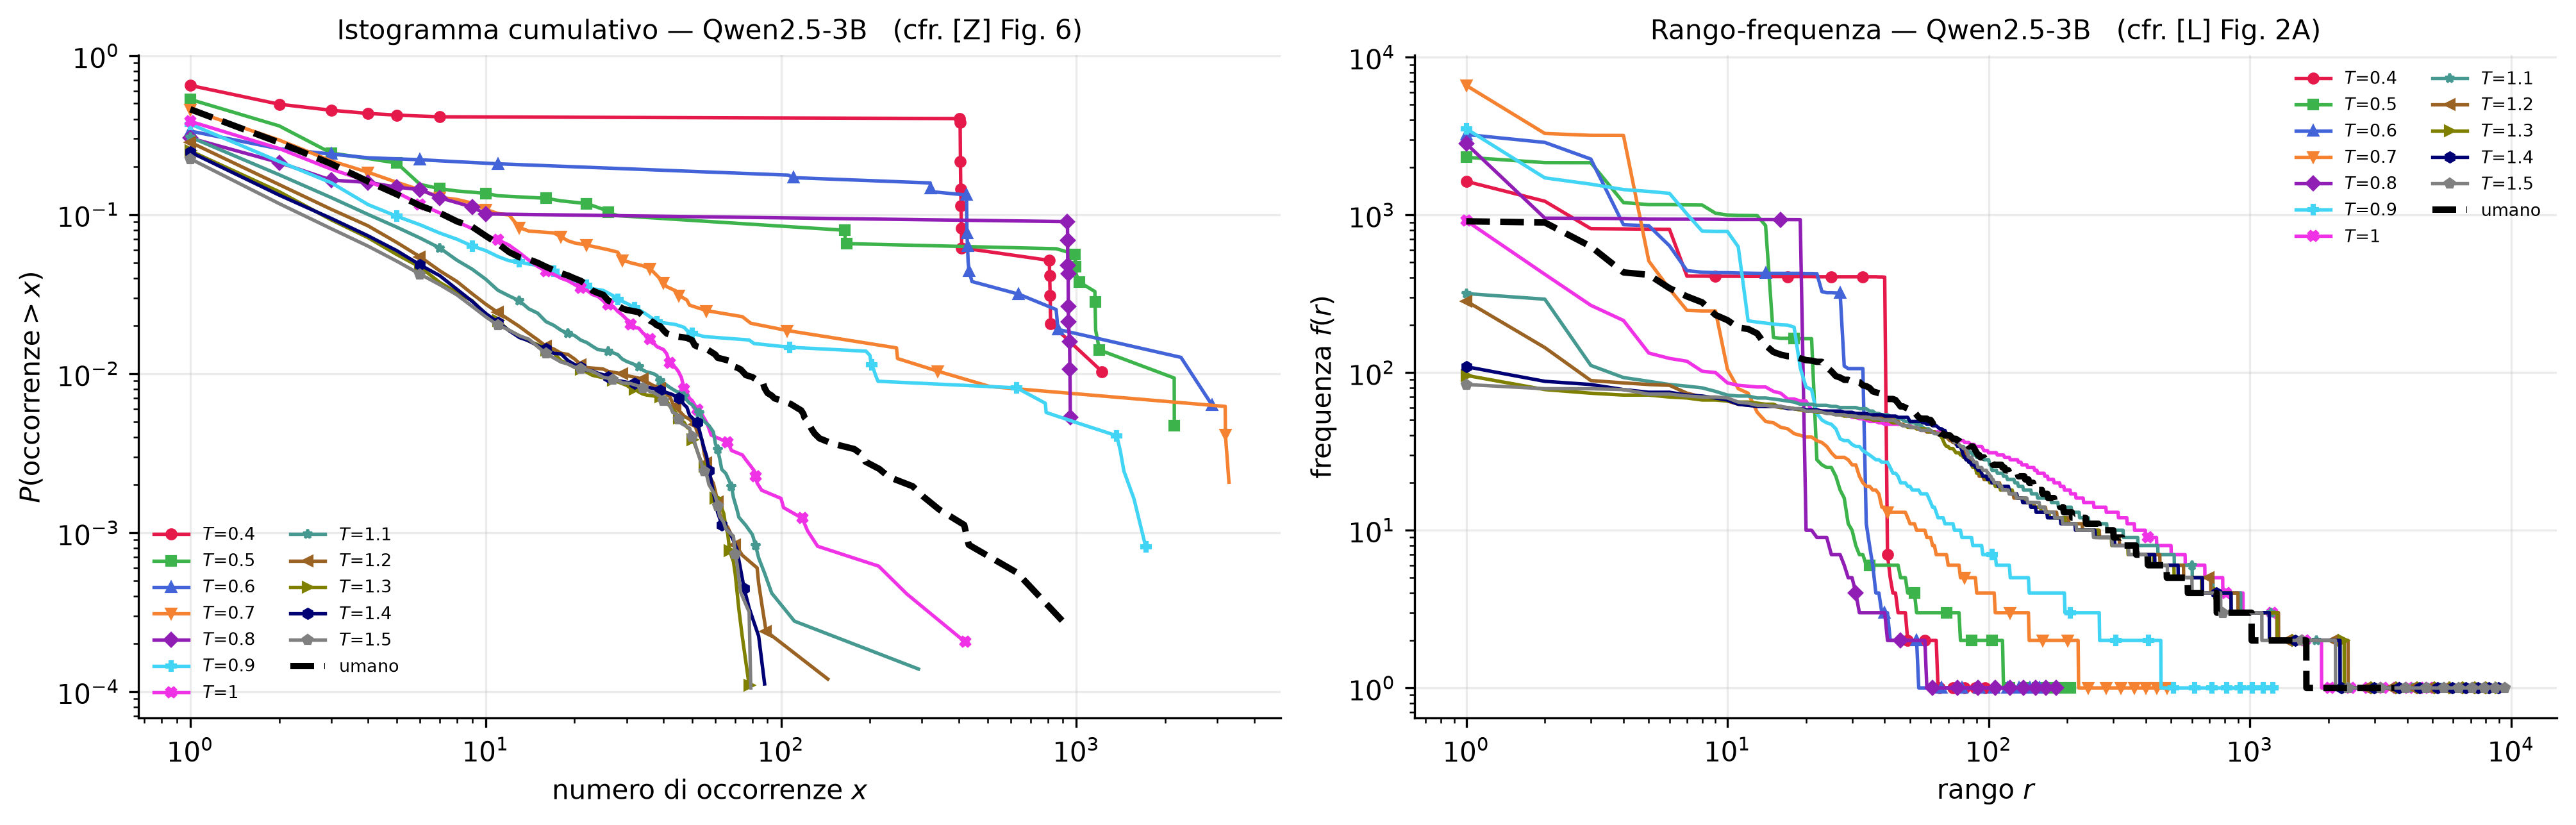
\includegraphics[width=\textwidth]{figure/cap4_zipf_cumulativo_Qwen25_3B.png}
  \caption{Istogrammi cumulativi delle frequenze dei token per il modello
  Qwen2.5-3B, una curva per temperatura. A bassa temperatura la curva è quasi
  verticale, perché pochi token coprono l'intero documento; ad alta temperatura
  è quasi orizzontale, perché quasi ogni token compare una volta sola. Solo
  nella regione intermedia la curva si avvicina alla retta che in coordinate
  bilogaritmiche corrisponde a una legge di potenza.}
  \label{fig:zipf-cum}
\end{figure}

L'esponente da solo non basta a descrivere questo comportamento, ed è la ragione
per cui nel §\ref{sec:zipf} è stato introdotto il MAPE: una curva può avere la
pendenza corretta e una curvatura marcata, e in tal caso l'esponente stimato non
descrive nulla. La Figura~\ref{fig:zipf-vs-T} riporta entrambe le quantità in
funzione della temperatura.

\begin{figure}[htbp]
  \centering
  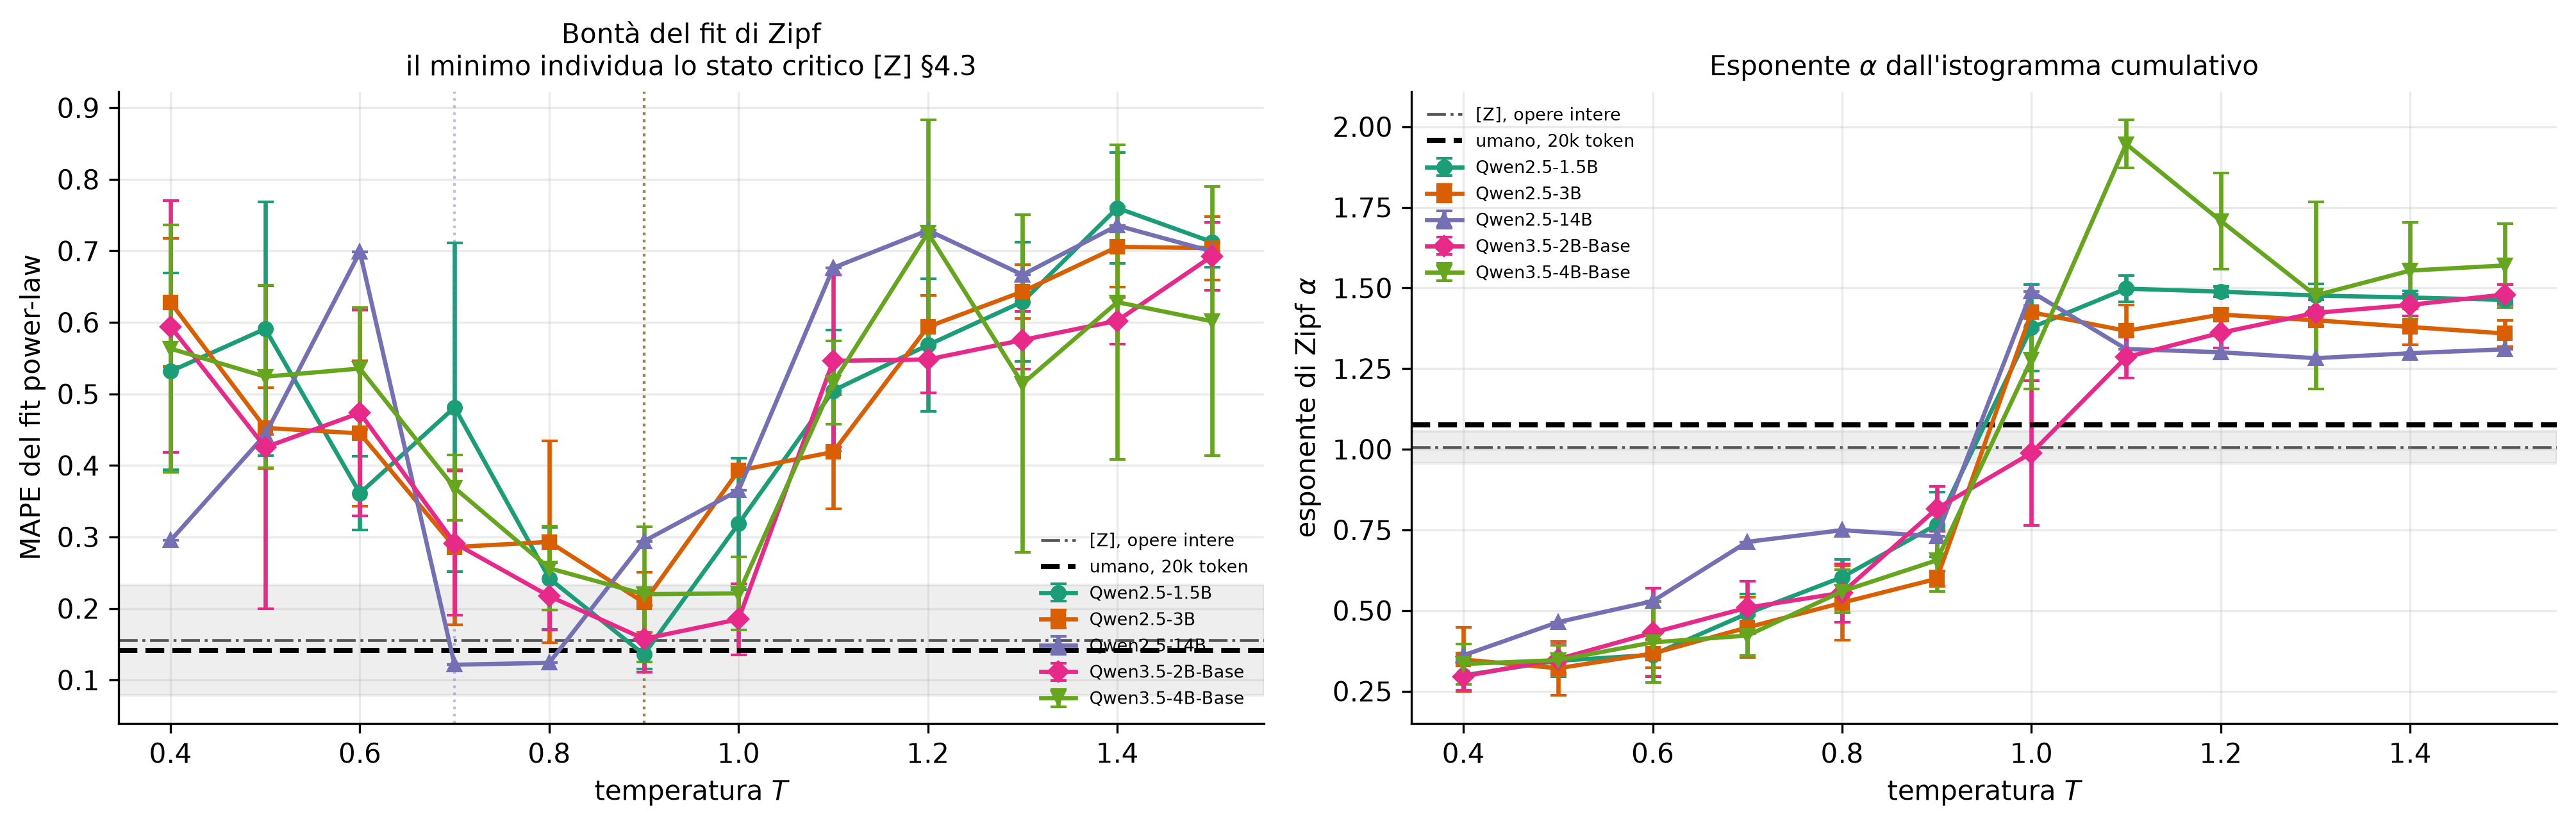
\includegraphics[width=\textwidth]{figure/cap4_zipf_vs_T.png}
  \caption{Bontà del fit e esponente della legge di Zipf in funzione della
  temperatura, per tutti e cinque i modelli. La banda grigia è il valore
  pubblicato su testi letterari interi, la linea nera tratteggiata la baseline
  umana misurata alla lunghezza di lavoro.}
  \label{fig:zipf-vs-T}
\end{figure}

Il MAPE ha un minimo pronunciato, che cade a $T = 0.9$ per quattro modelli su
cinque e a $T = 0.7$ per il modello da 14 miliardi di parametri. È il
risultato centrale della sezione: esiste una temperatura alla quale la
distribuzione delle frequenze del testo generato è più vicina a una legge di
potenza, e ai due lati di essa l'aderenza peggiora rapidamente.

Al minimo il MAPE del modello esemplare vale $0.208$. I due termini di
riferimento sono la baseline umana misurata alla stessa lunghezza, che vale
$0.141$, e il valore $0.156 \pm 0.077$ che~\cite{mikhaylovskiy2025zipf} riporta
su un corpus di sei opere letterarie in cinque lingue. Che i due riferimenti
umani cadano tanto vicini è una verifica indipendente della taratura della
baseline: sono ottenuti con tokenizzatori diversi, su testi diversi e di
lunghezza diversa, e la deriva documentata nella
Figura~\ref{fig:dimensione-finita} non rendeva scontato l'accordo.

Il valore del modello va letto contro tre metri diversi, e il giudizio che se ne
ricava non è lo stesso. Rispetto al modello stesso, $0.208$ è un risultato
netto: alle due estremità dell'intervallo lo stesso modello dà $0.628$ e
$0.704$, cioè un errore di fit tre volte più grande. Rispetto al testo umano è
invece una mezza vittoria: $0.208$ è circa una volta e mezza $0.141$, e resta
dentro la banda pubblicata solo perché quella banda è larga, sfiorandone il
margine superiore $0.233$. Rispetto agli altri modelli, infine, è un risultato
mediocre. La Tabella~\ref{tab:mape-minimi} riporta i cinque minimi: due modelli
scendono sotto il valore umano e un terzo vi si accosta, con $0.158$ contro
$0.141$, mentre il modello esemplare e il Qwen3.5-4B restano sopra.

\begin{table}[htbp]
\centering
\small
\begin{tabular}{@{}lrr@{}}
\toprule
Modello & $T$ del minimo & MAPE al minimo \\
\midrule
Qwen2.5-14B      & 0.7 & 0.121 \\
Qwen2.5-1.5B     & 0.9 & 0.136 \\
Qwen3.5-2B-Base  & 0.9 & 0.158 \\
Qwen2.5-3B       & 0.9 & 0.208 \\
Qwen3.5-4B-Base  & 0.9 & 0.220 \\
\midrule
testo umano      & --- & 0.141 \\
\bottomrule
\end{tabular}
\caption{Valore minimo del MAPE e temperatura alla quale viene raggiunto, per
ciascun modello, con la baseline umana misurata alla stessa lunghezza. Il
minimo esiste per tutti e cinque, ma solo tre modelli lo portano al livello del
testo umano o sotto. La riga del Qwen2.5-14B è ricavata da un solo campione per
temperatura e va letta con la cautela discussa nel testo.}
\label{tab:mape-minimi}
\end{table}

La prima riga della tabella richiede una precauzione. Il Qwen2.5-14B è l'unico
modello con un solo campione per temperatura, contro i tre o cinque degli altri,
e la sua curva del MAPE non è regolare da nessuno dei due lati del minimo: vale
$0.295$ a $T = 0.4$, sale a $0.698$ a $T = 0.6$ e scende a $0.121$ a $T = 0.7$,
cioè peggiora di un fattore due e migliora di un fattore sei in due passi
consecutivi. Negli altri quattro modelli la dispersione fra campioni alla stessa
temperatura va da $0.046$ a $0.230$ attorno a $T = 0.7$, mentre la distanza fra
il minimo del 14B e il suo valore a $T = 0.9$ vale $0.173$: sta dentro
quell'intervallo. Con una sola realizzazione la posizione del minimo non è
risolvibile, e il valore $T = 0.7$ va letto come compatibile con il $T = 0.9$
degli altri quattro anziché come uno spostamento reale. La stessa cautela vale
per la profondità: $0.121$ è il minimo più basso dei cinque ed è anche il meno
affidabile, mentre il $0.136$ del Qwen2.5-1.5B poggia su cinque campioni con
dispersione $0.020$ ed è l'unico caso in cui il primato sul testo umano è
sostenuto da repliche.

La posizione del minimo va confrontata con quella riportata nella fonte.
In~\cite{mikhaylovskiy2025zipf} il minimo del MAPE cade fra $t = 1.0$ e
$t = 1.2$ per tutti i modelli tranne i Llama più grandi, mentre qui cade a
$T = 0.9$ per quattro modelli su cinque. Lo scarto è nella direzione prevista
dall'effetto del prompt descritto nel §\ref{sec:protocollo}, che abbassa
l'errore del fit soprattutto alle basse temperature e sposta quindi il minimo
verso sinistra.

Ne segue una distinzione che vale per tutto il seguito. L'esistenza
di una temperatura ottimale è un fatto generale, comune a tutti e cinque i
modelli; la qualità dell'ottimo, cioè quanto il testo generato in quel punto
somigli davvero a un testo umano, varia da modello a modello e non è garantita.
Il modello scelto come esemplare non è fra quelli che ci riescono, e i grafici
del corpo del capitolo vanno letti tenendolo presente.

L'esponente $\alpha$ racconta la stessa storia da un'altra angolazione. Per il
modello esemplare passa da $0.35$ a $T = 0.4$, valore che corrisponde a una
distribuzione dominata da pochissimi tipi, a $1.36$ a $T = 1.5$, dove più di tre
quarti dei tipi compaiono una volta sola.\footnote{Un tipo che compare una sola
volta nel testo si dice \emph{hapax}. Gli hapax sono normalmente la maggioranza
dei tipi ma una piccola parte delle occorrenze: nella baseline umana usata qui
sono il $54\%$ dei tipi e il $10\%$ dei token, mentre a $T = 1.5$ il modello
esemplare arriva al $77\%$ dei tipi e al $37\%$ dei token.} La transizione non è
graduale: fra $T = 0.9$ e $T = 1.0$ l'esponente salta da $0.60$ a $1.43$,
attraversando in un solo passo il valore umano $1.076$, per poi assestarsi
attorno a $1.4$ senza più avvicinarvisi.

% ---------------------------------------------------------------------
\section{Legge di Heaps e descrittore \texorpdfstring{$R$}{R}}
\label{sec:heaps-risultati}

Le curve di crescita del vocabolario rendono immediatamente evidente perché il
§\ref{sec:heaps} abbia dovuto introdurre un descrittore alternativo all'esponente di
Heaps.

\begin{figure}[htbp]
  \centering
  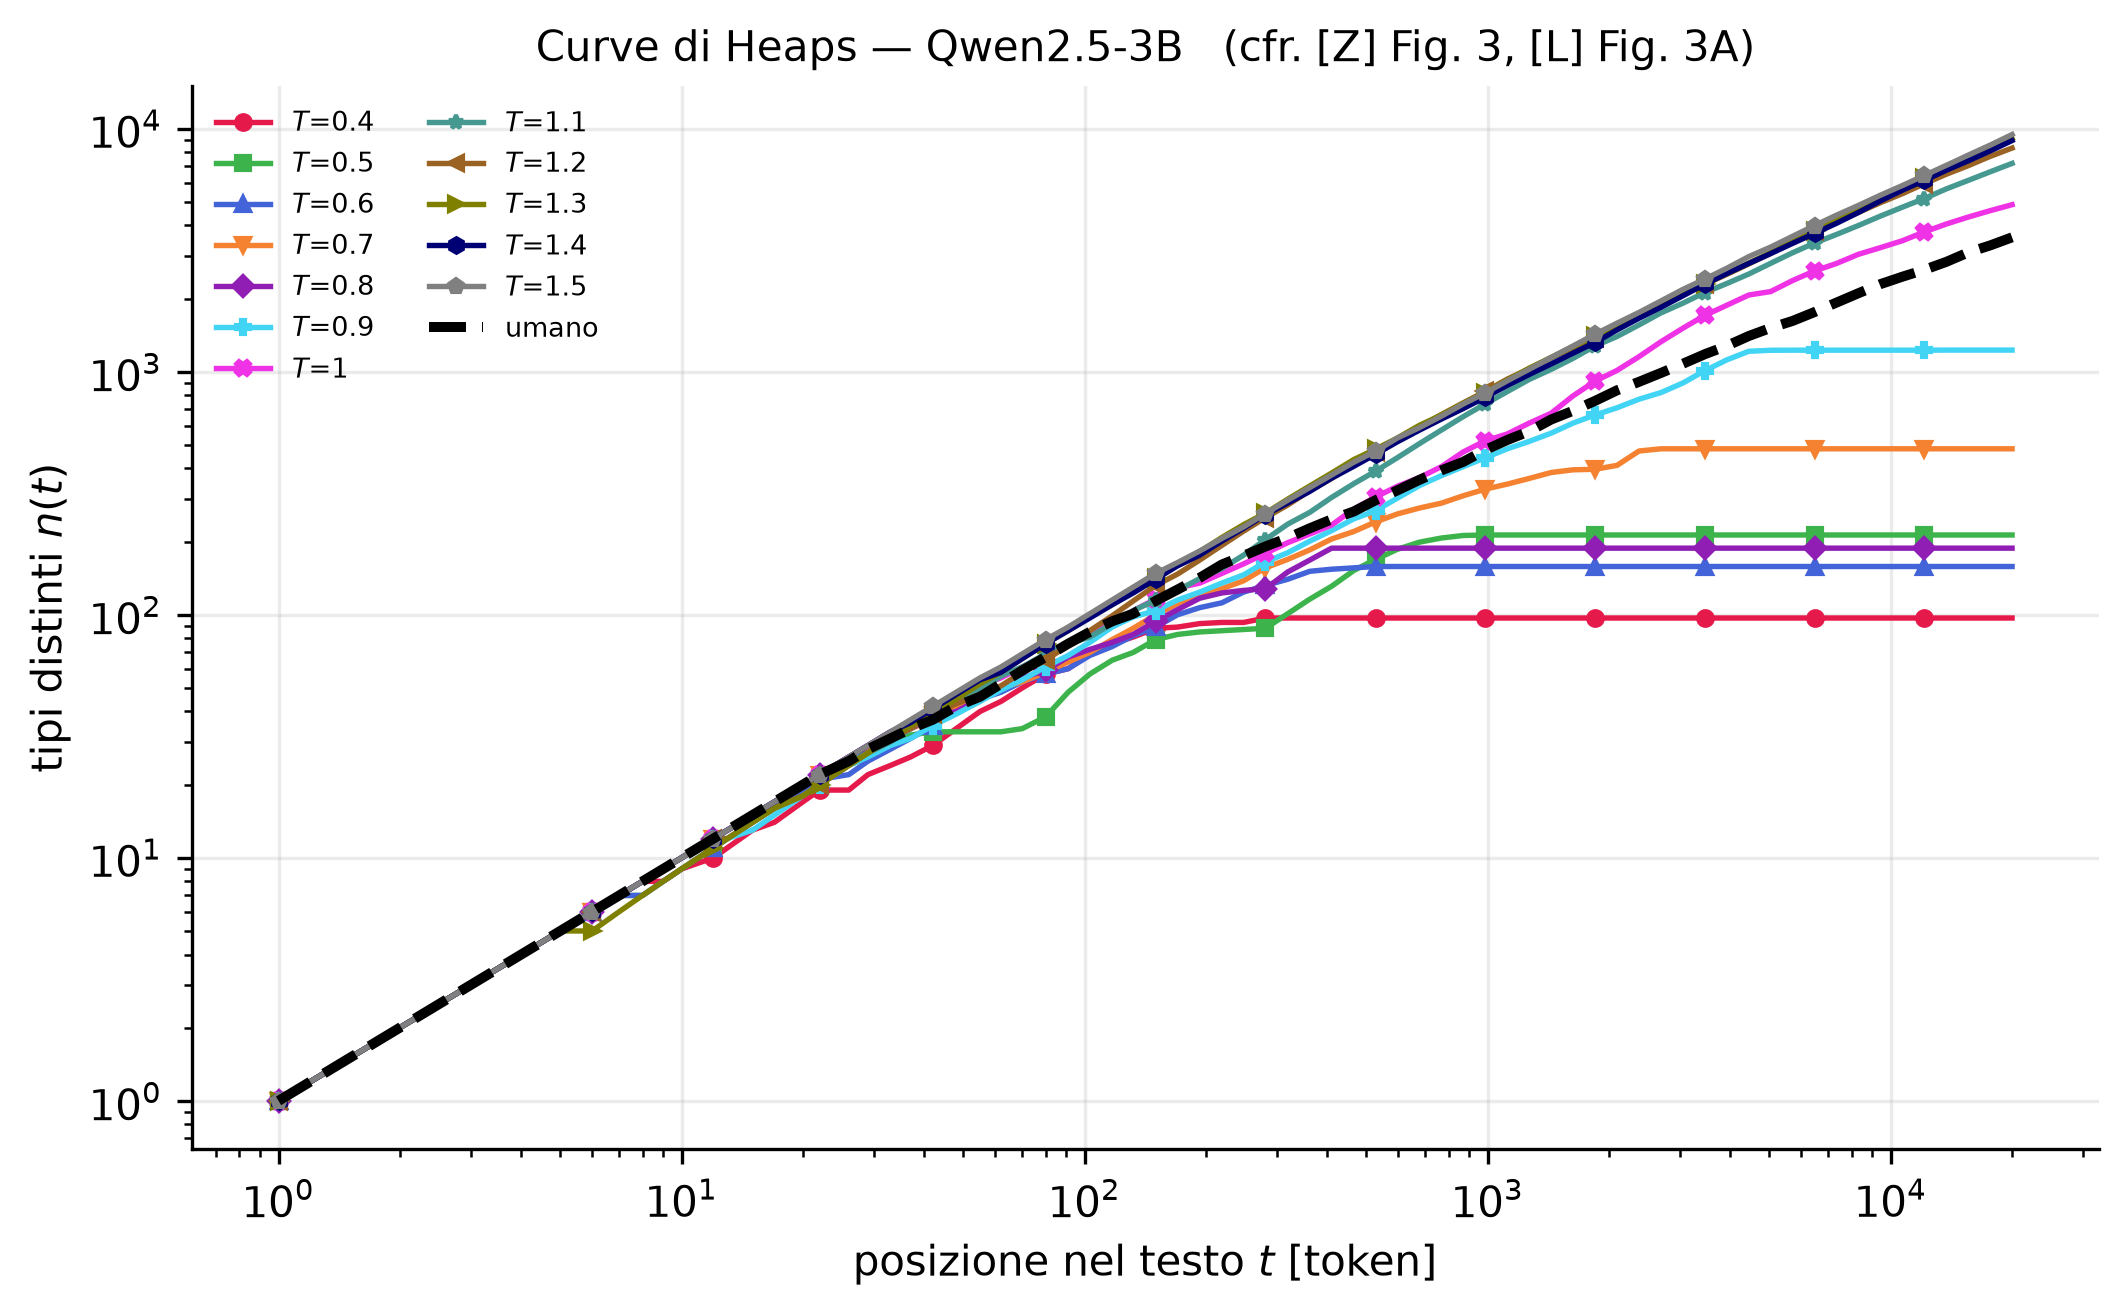
\includegraphics[width=0.86\textwidth]{figure/cap4_heaps_curve_Qwen25_3B.png}
  \caption{Crescita del vocabolario per il modello Qwen2.5-3B. Alle temperature
  basse la curva si appiattisce dopo poche migliaia di token: il modello ha
  smesso di produrre tipi nuovi. Alle temperature alte cresce quasi linearmente.
  In nessuno dei due casi la curva è una legge di potenza, e stimarne
  l'esponente restituisce un numero privo di contenuto.}
  \label{fig:heaps-curve}
\end{figure}

La Figura~\ref{fig:heaps-R} riporta il descrittore $R$, l'esponente $\gamma_H$
e il rapporto fra tipi e occorrenze in funzione della temperatura. I tre
andamenti sono concordi: per il modello esemplare $\gamma_H$ passa da $0.001$
a $T = 0.4$, dove la curva è piatta e il vocabolario non cresce affatto, a
$0.806$ a $T = 1.5$, attraversando il valore umano $0.668$ poco sopra $T =
0.9$. Il descrittore $R$ passa da $0.003$ a $0.688$ e incrocia il valore umano
$0.507$ attorno a $T = 1.05$.

Il terzo pannello riporta la quantità più elementare delle tre, il rapporto fra
il numero di tipi distinti e il numero di occorrenze, e serve da controllo sulle
altre due. A differenza di $\gamma_H$ e di $R$ non richiede alcun fit né alcuna
partizione del documento, quindi non può essere alterato da un modello mal
specificato: se le tre curve concordano, l'andamento non è un artefatto della
procedura di stima. Per il modello esemplare passa da $0.007$ a $T = 0.4$ a
$0.474$ a $T = 1.5$, e attraversa il valore umano $0.179$ fra $T = 0.9$ e
$T = 1.0$, cioè nello stesso punto delle altre due misure. Il pannello mostra
però anche in che senso l'accordo con il testo umano sia solo locale: sopra
$T = 1.1$ il rapporto supera il doppio del valore umano e continua a crescere,
mentre $\gamma_H$ resta stabile attorno a $0.8$. Le due misure smettono di dire
la stessa cosa non appena il vocabolario si allarga oltre quello di un romanzo.

\begin{figure}[htbp]
  \centering
  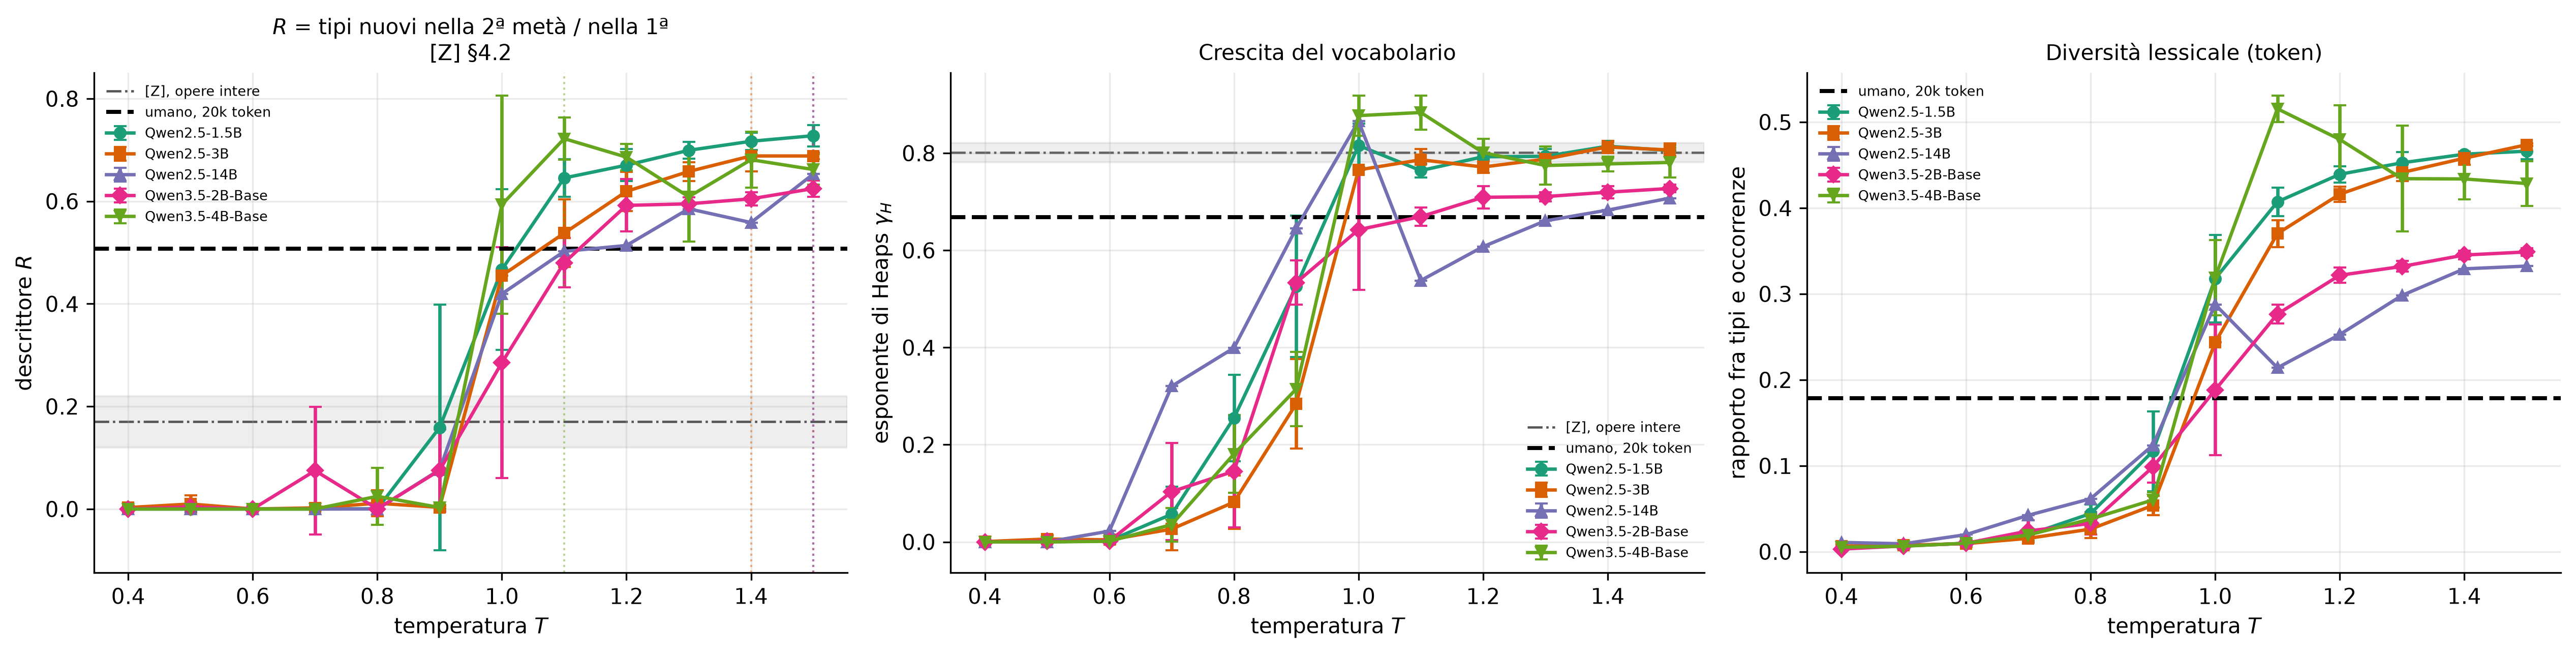
\includegraphics[width=\textwidth]{figure/cap4_heaps_R_vs_T.png}
  \caption{Descrittore $R$, esponente di Heaps e rapporto fra tipi e occorrenze
  in funzione della temperatura. La banda grigia riporta i valori pubblicati su
  opere intere, che per le ragioni discusse nel §\ref{sec:scelte} non sono un
  termine di confronto diretto.}
  \label{fig:heaps-R}
\end{figure}

% ---------------------------------------------------------------------
\section{Correlazioni a lungo raggio}
\label{sec:dfa-risultati}

Ogni documento viene convertito nella successione numerica definita nel
§\ref{sec:dfa}: ogni carattere è sostituito dal proprio rango di frequenza nel
documento, $1$ al più frequente, $2$ al secondo, e così via. È su quella
successione che si misura l'esponente della fluttuazione. Il detrending è
quadratico: il §\ref{sec:robustezza} documenta il confronto con quello lineare e
la ragione della scelta, cioè che alle basse temperature i documenti non sono
stazionari e un polinomio di primo grado non assorbe la deriva della
composizione dei caratteri. Il primo controllo riguarda il null model: la stessa
analisi condotta sui documenti rimescolati deve restituire un esponente pari a
$1/2$.


La Figura~\ref{fig:dfa} riporta le curve di fluttuazione e l'esponente in
funzione della temperatura. L'esponente ha un massimo a $T = 1.0$, dove vale
$0.719$ in media su tutti i modelli, superiore al valore umano di $0.579$;
decresce poi verso $0.53$ alle temperature più alte, avvicinandosi al valore del
rimescolamento senza raggiungerlo.

\begin{figure}[htbp]
  \centering
  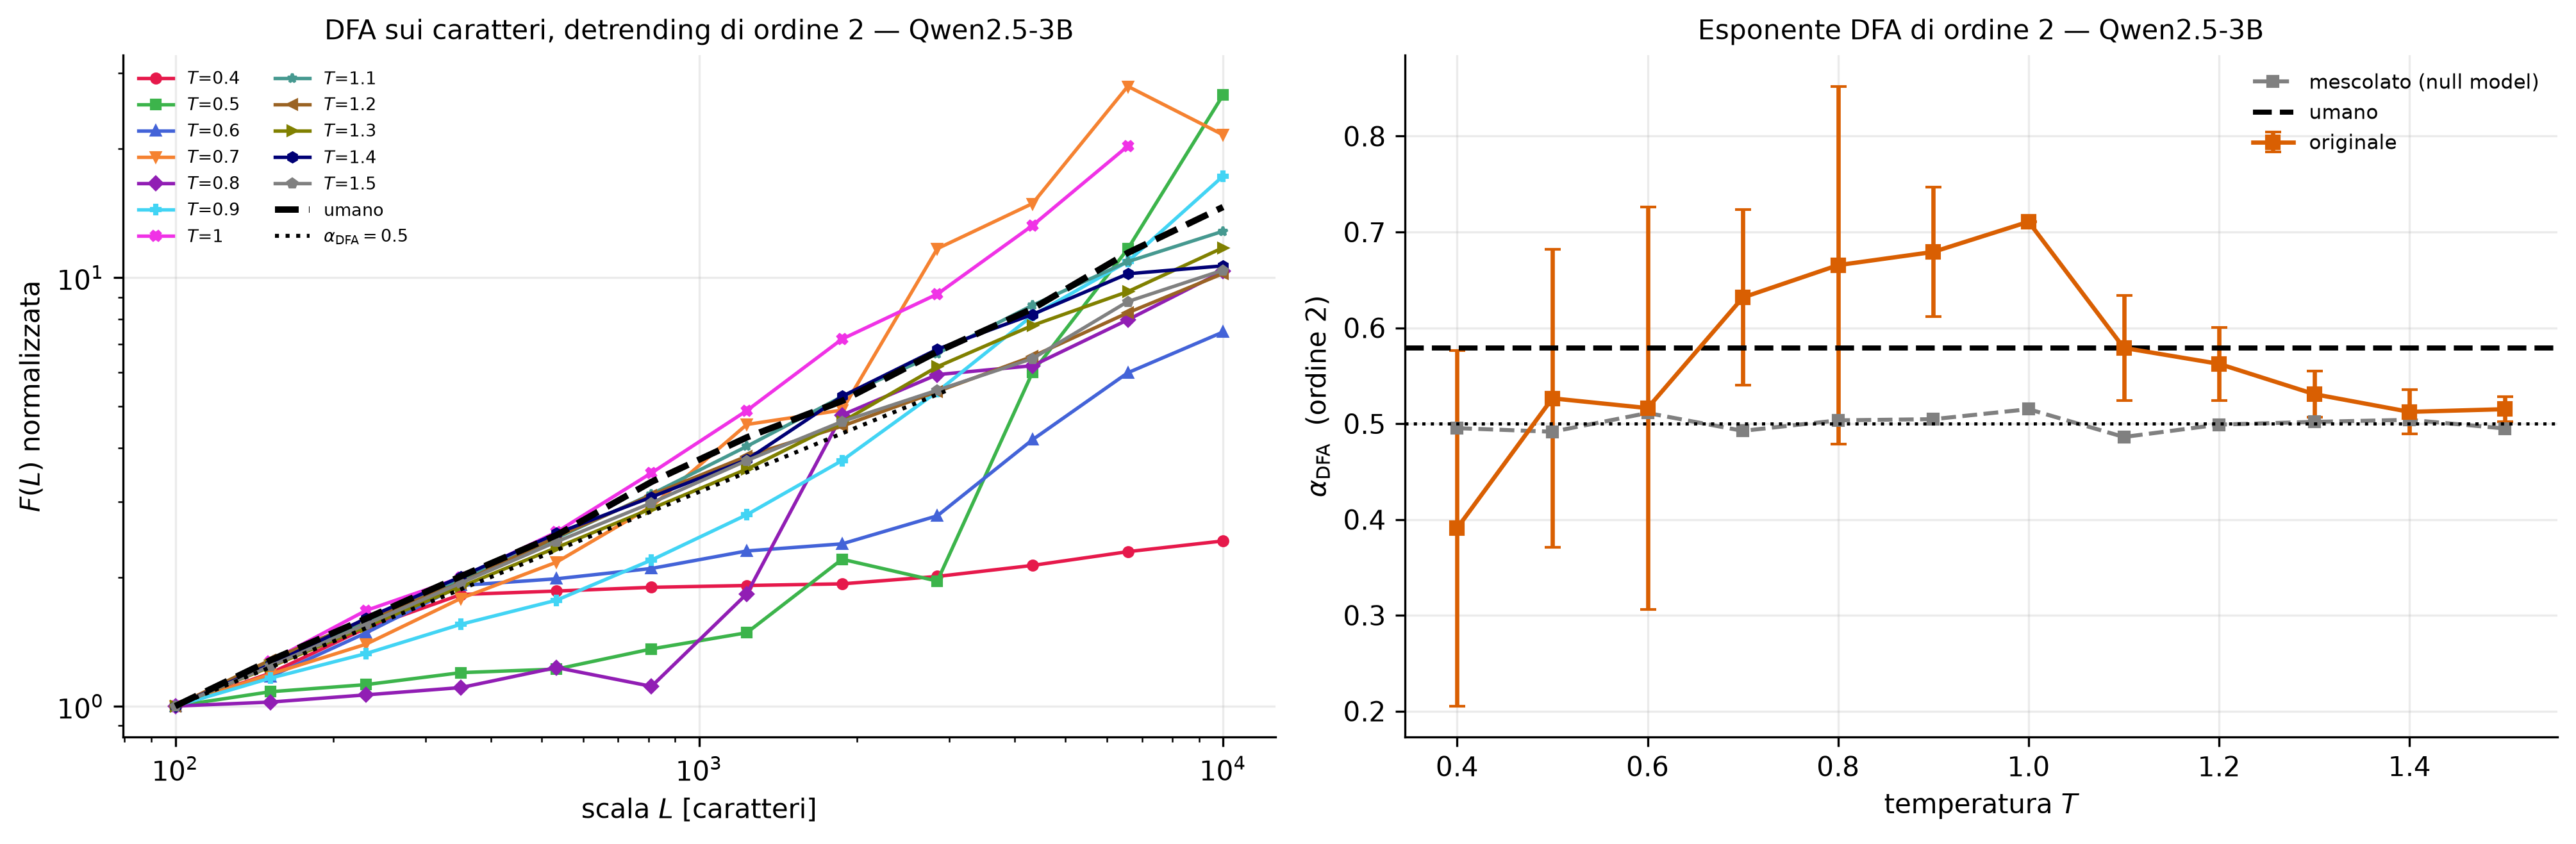
\includegraphics[width=\textwidth]{figure/cap4_dfa_Qwen25_3B_o2.png}
  \caption{Fluttuazione detrendizzata per il modello Qwen2.5-3B, con detrending
  quadratico. A sinistra $F(s)$ in funzione della scala, una curva per
  temperatura, con la pendenza di riferimento $\alpha_{\mathrm{DFA}} = 1/2$; a
  destra l'esponente in funzione della temperatura, con il null model
  rimescolato e la baseline umana.}
  \label{fig:dfa}
\end{figure}

\paragraph{La dispersione è il vero segnale.}
Il valore medio dell'esponente nasconde il fenomeno più informativo, ed è un
fenomeno già osservato: sulle reti LSTM~\cite{lippi2019} riporta che le stime
sui singoli campioni sono molto disperse attorno a $T = 0.5$ e strettamente
raccolte attorno alla media a $T = 1.0$. Gli stessi dati mostrano qui lo stesso
comportamento su architetture transformer. La deviazione standard fra documenti
passa da $0.219$ a $T = 0.4$ a $0.022$ a $T = 1.4$: alle basse temperature la
stima è dieci volte più dispersa. A $T = 0.4$ i cinque documenti del modello
esemplare danno esponenti compresi fra $0.16$ e $0.66$, cioè coprono
l'intervallo fra la saturazione e il valore umano; sull'insieme dei cinque
modelli l'escursione va da $0.07$ a $0.89$.

Questo comportamento è coerente con il caso limite discusso nel
§\ref{sec:ponte}. Quando il testo entra in un ciclo di ripetizione, il profilo
cumulato oscilla invece di allontanarsi dall'origine e la fluttuazione satura:
l'esponente crolla. Il crollo dipende però dalla lunghezza del ciclo rispetto
alle scale analizzate, che varia da documento a documento, e non tutti i testi
ripetitivi lo manifestano.

I dati permettono di precisare la relazione, che è a senso unico. Tutti e
diciannove i documenti con $\alpha_{\mathrm{DFA}} < 0.3$ si trovano a
$T \le 0.6$ e hanno una quota media di 8-grammi ripetuti pari a $0.984$: un
esponente collassato implica dunque ripetizione conclamata. Il viceversa non
vale: fra gli 82 documenti con quota di 8-grammi ripetuti superiore a $0.9$,
soltanto 33 hanno un esponente inferiore a $1/2$, e la correlazione di rango fra
le due quantità non è significativa
($\rho = +0.03$, $p = 0.61$). La ripetizione è quindi condizione necessaria ma
non sufficiente al collasso dell'esponente.

Ne segue una conseguenza metodologica. Alle basse temperature
$\alpha_{\mathrm{DFA}}$ non è un indicatore affidabile di correlazione a lungo
raggio, né lo è il suo valore medio; è la sua dispersione a segnalare il regime.
Il controllo sull'ordine del detrending riportato nel §\ref{sec:robustezza}
punta nella stessa direzione, poiché lo scarto fra i due ordini è massimo
proprio nell'intervallo $T \in [0.5, 0.8]$ e trascurabile altrove.

% ---------------------------------------------------------------------
\section{Entropia, divergenza dal testo umano e plagio}
\label{sec:entropia-risultati}

Le sezioni precedenti confrontano il testo generato con quello umano una misura
alla volta. La divergenza di Kullback--Leibler introdotta nel
§\ref{sec:crossparsing} permette invece un confronto diretto fra i due testi,
senza passare per un descrittore intermedio, ed è per questa ragione il criterio
più stringente del capitolo: non dipende da soglie teoriche né dalla scelta di
quale proprietà misurare.


La divergenza ha un minimo netto, che cade a $T = 0.9$ per quattro modelli su
cinque e a $T = 1.0$ per Qwen3.5-4B-Base. Nessuna delle \num{242} stime risulta
negativa, il che conferma sui dati reali la proprietà dello stimatore verificata
nel §\ref{sec:validazione}.

Il valore al minimo varia molto fra i modelli: $0.096$ bit per carattere per il
modello da 14 miliardi di parametri, $0.232$ e $0.245$ per i due Qwen3.5,
$0.321$ per il modello da 1.5 miliardi e $0.914$ per quello da 3 miliardi. La
posizione del minimo è dunque comune, la sua profondità no: fra il modello che
si avvicina di più al testo umano e quello che ci riesce meno corre quasi un
fattore dieci. La profondità non segue però la dimensione. La correlazione di
rango con il numero di parametri vale $\rho = -0.50$ con $p = 0.39$ su cinque
modelli, e il valore peggiore appartiene al modello da 3 miliardi anziché al più
piccolo: quanto un modello si avvicini al testo umano nel proprio punto migliore
è una proprietà del singolo modello, non della sua scala, almeno con la potenza
statistica qui disponibile. Vale inoltre la cautela imposta dal
§\ref{sec:robustezza}, poiché il modello da 14 miliardi dispone di un solo
campione per temperatura e il suo valore non è corredato da una stima della
dispersione.

L'entropia stimata per compressione mostra la transizione in modo ancora più
brusco. Per il modello esemplare la mediana vale $0.001$ bit per carattere
fino a $T = 0.8$, perché il testo ripetitivo è essenzialmente incomprimibile
oltre la prima occorrenza del ciclo e non trasporta informazione; sale poi a
$0.332$ in media a $T = 0.9$ e supera $4$ da $T = 1.0$ in poi, contro i $2.23$
del testo umano. Fra $T = 0.6$ e $T = 0.9$ la media si stacca dalla mediana
perché un documento per temperatura esce dal ciclo prima degli altri, e il
valore isolato di $5.77$ che il modello esemplare raggiunge a $T = 1.0$
proviene dall'unico documento sopravvissuto a quella temperatura: è la stessa
dispersione descritta nel §\ref{sec:dfa-risultati}, e conferma che nel regime
periodico il valore medio non descrive alcun documento. Il passaggio dal
regime a entropia trascurabile a quello a entropia superiore a quella umana si
consuma comunque entro due passi di temperatura.

% ---------------------------------------------------------------------
\section{Struttura misurata per compressione}
\label{sec:compressione-risultati}

Le misure basate su compressione del §\ref{sec:compressione} non richiedono di
scegliere un'unità di analisi né di stimare un esponente: operano direttamente
sui byte del testo. Costituiscono quindi un controllo indipendente da tutte le
scelte metodologiche discusse finora.

\begin{figure}[htbp]
  \centering
  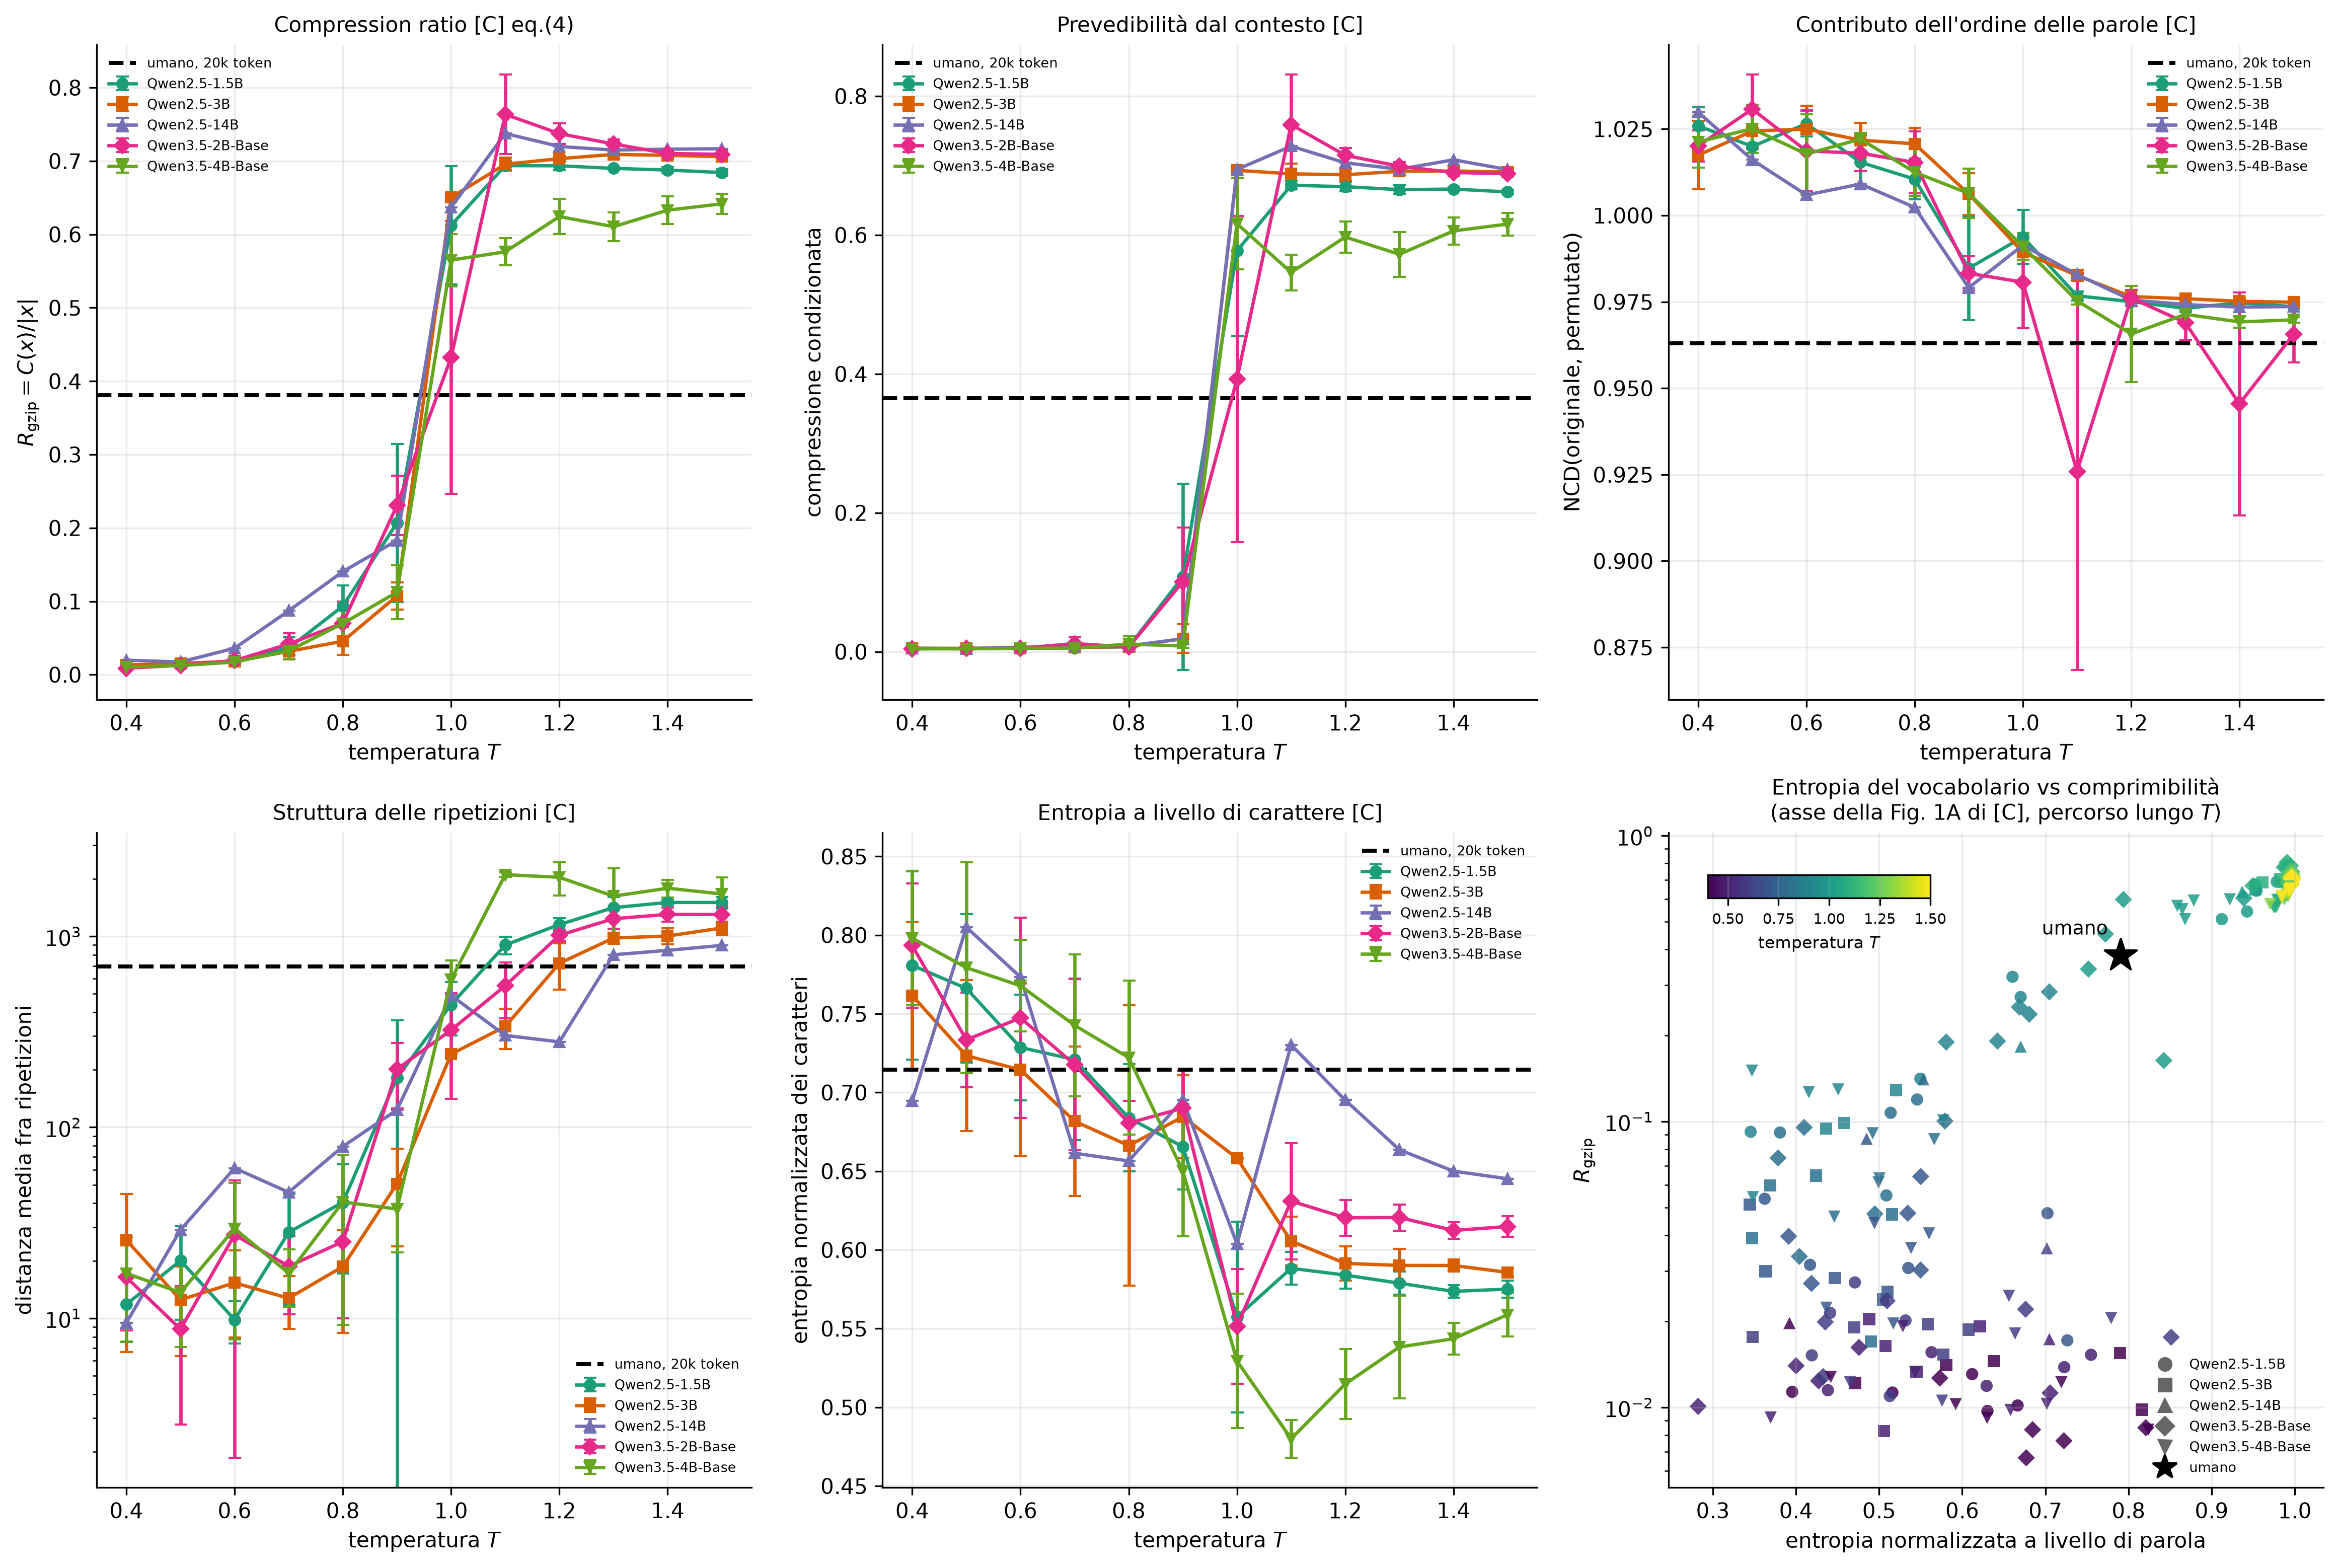
\includegraphics[width=\textwidth]{figure/cap4_compressione.png}
  \caption{Sei misure basate su compressione. Le prime cinque sono riportate in
  funzione della temperatura; l'ultima, in basso a destra, riporta il rapporto
  di compressione contro
  l'entropia normalizzata a livello di parola: è il piano della Figura~1A
  di~\cite{hadad2026}, percorso qui facendo variare la temperatura, con il testo
  umano segnato da una stella. In quel pannello il colore codifica la
  temperatura e la forma del marcatore il modello, e la scala verticale è
  logaritmica.}
  \label{fig:compressione}
\end{figure}

Il rapporto di compressione è la misura che separa i regimi in modo più netto di
tutte le altre. Per il modello esemplare passa da $0.013$ a $T = 0.4$ a $0.107$
a $T = 0.9$ e a $0.650$ a $T = 1.0$: un fattore cinquanta fra i due estremi, con
un salto di un fattore sei concentrato in un singolo passo di temperatura. Il
valore umano è $0.381$, e viene attraversato fra $T = 0.9$ e $T = 1.0$ come
tutte le altre misure del capitolo.

Il lavoro di~\cite{hadad2026} riporta che il testo generato è più regolare e
più comprimibile di quello umano, mentre qui il rapporto di compressione
supera il valore umano sopra $T = 1.0$. Le due osservazioni non sono in
contrasto, perché descrivono regioni diverse dello stesso asse: sotto la
transizione il testo generato è molto più comprimibile del testo umano,
$0.013$ contro $0.381$, ed è il regime in cui i modelli operano con le
impostazioni ordinarie; sopra la transizione la comprimibilità cade perché il
testo cessa di essere linguaggio, non perché acquisti struttura.

La compressione condizionata si comporta in modo analogo ma dice qualcosa di
diverso. Fino a $T = 0.9$ vale meno di $0.02$: la seconda metà del documento è
quasi interamente prevedibile dalla prima, come è ovvio in un testo che ripete
lo stesso ciclo. Da $T = 1.0$ sale a circa $0.69$, quasi il doppio del valore
umano $0.365$: la seconda metà è ora \emph{meno} prevedibile dalla prima di
quanto lo sia in un romanzo. Fra i due regimi non esiste una temperatura in cui
la predicibilità dal contesto assomigli a quella del testo umano.

Il salto oltre il valore umano non è una particolarità del modello esemplare. La
mediana su tutti e cinque i modelli passa da $0.015$ a $T = 0.9$ a $0.627$ a
$T = 1.0$, e il singolo modello che si avvicina di più al valore umano da sotto,
il Qwen3.5-2B-Base con $0.135$, lo scavalca comunque in un passo arrivando a
$0.430$. Nessuno dei cinque si ferma sul valore umano, ed è l'unica delle misure
di questo capitolo per cui ciò accade.

\paragraph{Il piano entropia--comprimibilità.}
Il pannello in basso a destra della Figura~\ref{fig:compressione} colloca i
documenti nel piano definito da~\cite{hadad2026}, percorso qui da un modello
reale al variare di un solo parametro anziché da distribuzioni artificiali, con
il testo umano in posizione intermedia. L'asse verticale è logaritmico perché il rapporto di compressione
non si annulla mai: il valore più basso osservato è $0.0067$. Su un asse
lineare esteso fino a $0.81$, però, i 57 documenti che stanno fra $0.007$ e
$0.020$, quasi un quarto del totale, si sovrappongono tutti sulla linea dello
zero, e la loro struttura interna scompare. In scala logaritmica si vede
invece che occupano un intervallo di entropia molto ampio, da $0.28$ a $0.85$,
e la ragione è che le due grandezze misurano cose diverse. Il rapporto di
compressione dipende dalla ripetizione della sequenza: un testo che ripete
sempre lo stesso ciclo si comprime a poco più dell'un per cento della sua
dimensione, qualunque sia il numero di parole che il ciclo contiene.
L'entropia normalizzata dipende invece dalla forma della distribuzione delle
frequenze su quel vocabolario ridotto, che conta fra 37 e 235 tipi distinti.
Un ciclo lungo e vario e un ciclo corto e povero sono ugualmente comprimibili
ma hanno entropie molto diverse: da qui la dispersione orizzontale della
nuvola a bassa comprimibilità.

\paragraph{La lunghezza del ciclo, misurata.}
L'argomento appena esposto invoca una grandezza che le misure di questo capitolo
non contengono, la lunghezza del ciclo ripetuto, ed è quindi il caso di
misurarla. Sulla successione di parole di ciascun documento si cerca il più
piccolo sfasamento $L_{\mathrm{ciclo}}$ per cui l'accordo fra la parola in
posizione $i$ e quella in posizione $i - L_{\mathrm{ciclo}}$, calcolato sugli
ultimi venti giri, supera il novanta per cento. La finestra di verifica è locale
e commisurata al periodo candidato: su tutto il testo la prosa che precede il
ciclo diluirebbe la media, mentre su un suffisso lungo un ciclo che cambia
lentamente variante scende sotto soglia al proprio periodo e la supera a un
multiplo, restituendo un alias. La soglia è fissata al novanta e non al cento
per cento per tollerare i cicli non esattamente verbatim; l'accordo atteso per
caso in prosa inglese è circa $0.05$, quindi non vi sono falsi positivi.

Il criterio individua \num{113} documenti su \num{242}, e sono tutti a
$T \le 0.9$: la totalità fino a $T = 0.7$, il $95\%$ a $T = 0.8$, il $56\%$ a
$T = 0.9$ e nessuno da
$T = 1.0$ in poi. Coincidono con la nuvola a bassa comprimibilità: tutti e
cinquantasette i documenti con $R_{\mathrm{gzip}} < 0.02$ sono fra questi. Il
ciclo va da una sola parola a \num{248}, in caratteri da $9$ a \num{1127}, con
mediana di $16$ parole.

La Figura~\ref{fig:ciclo} riporta la relazione con le due grandezze del piano.
Con l'entropia di parola la correlazione di rango vale $\rho = +0.65$, e non è
un effetto della temperatura: calcolata fra documenti generati alla stessa
temperatura sale a $+0.69$, ed è positiva in tutti e sei i gruppi. Con il
rapporto di compressione, invece, non c'è relazione: $\rho = -0.15$ con
$p = 0.12$, e a temperatura fissata il segno si inverte, $+0.16$ con
$p = 0.11$. A parità di lunghezza del ciclo il rapporto di compressione varia di
un fattore compreso fra quattordici e ventisette.

Il meccanismo è quello anticipato sopra, e la misura lo rende esplicito: la
lunghezza del ciclo coincide quasi con il numero di tipi distinti che esso
contiene, $\rho = +0.84$, cosicché un ciclo corto concentra tutta la massa di
probabilità su poche parole e uno lungo la distribuisce. Gli estremi lo
mostrano nel modo più diretto: il ciclo più corto osservato è una sola parola,
ripetuta, con entropia $0.35$; il più lungo conta \num{248} parole e undici
tipi distinti, \emph{You are a bad father. You are a bad lover of children.
You are not to blame} con variazioni, con entropia $0.47$ e $R_{\mathrm{gzip}}
= 0.019$, cioè testo ancora ultracomprimibile. La lunghezza del ciclo spiega
dunque l'ordinamento lungo l'asse orizzontale del piano, non tutta la sua
dispersione: la regressione su $\log L_{\mathrm{ciclo}}$ rende conto del
$42\%$ della varianza dell'entropia.

\begin{figure}[htbp]
  \centering
  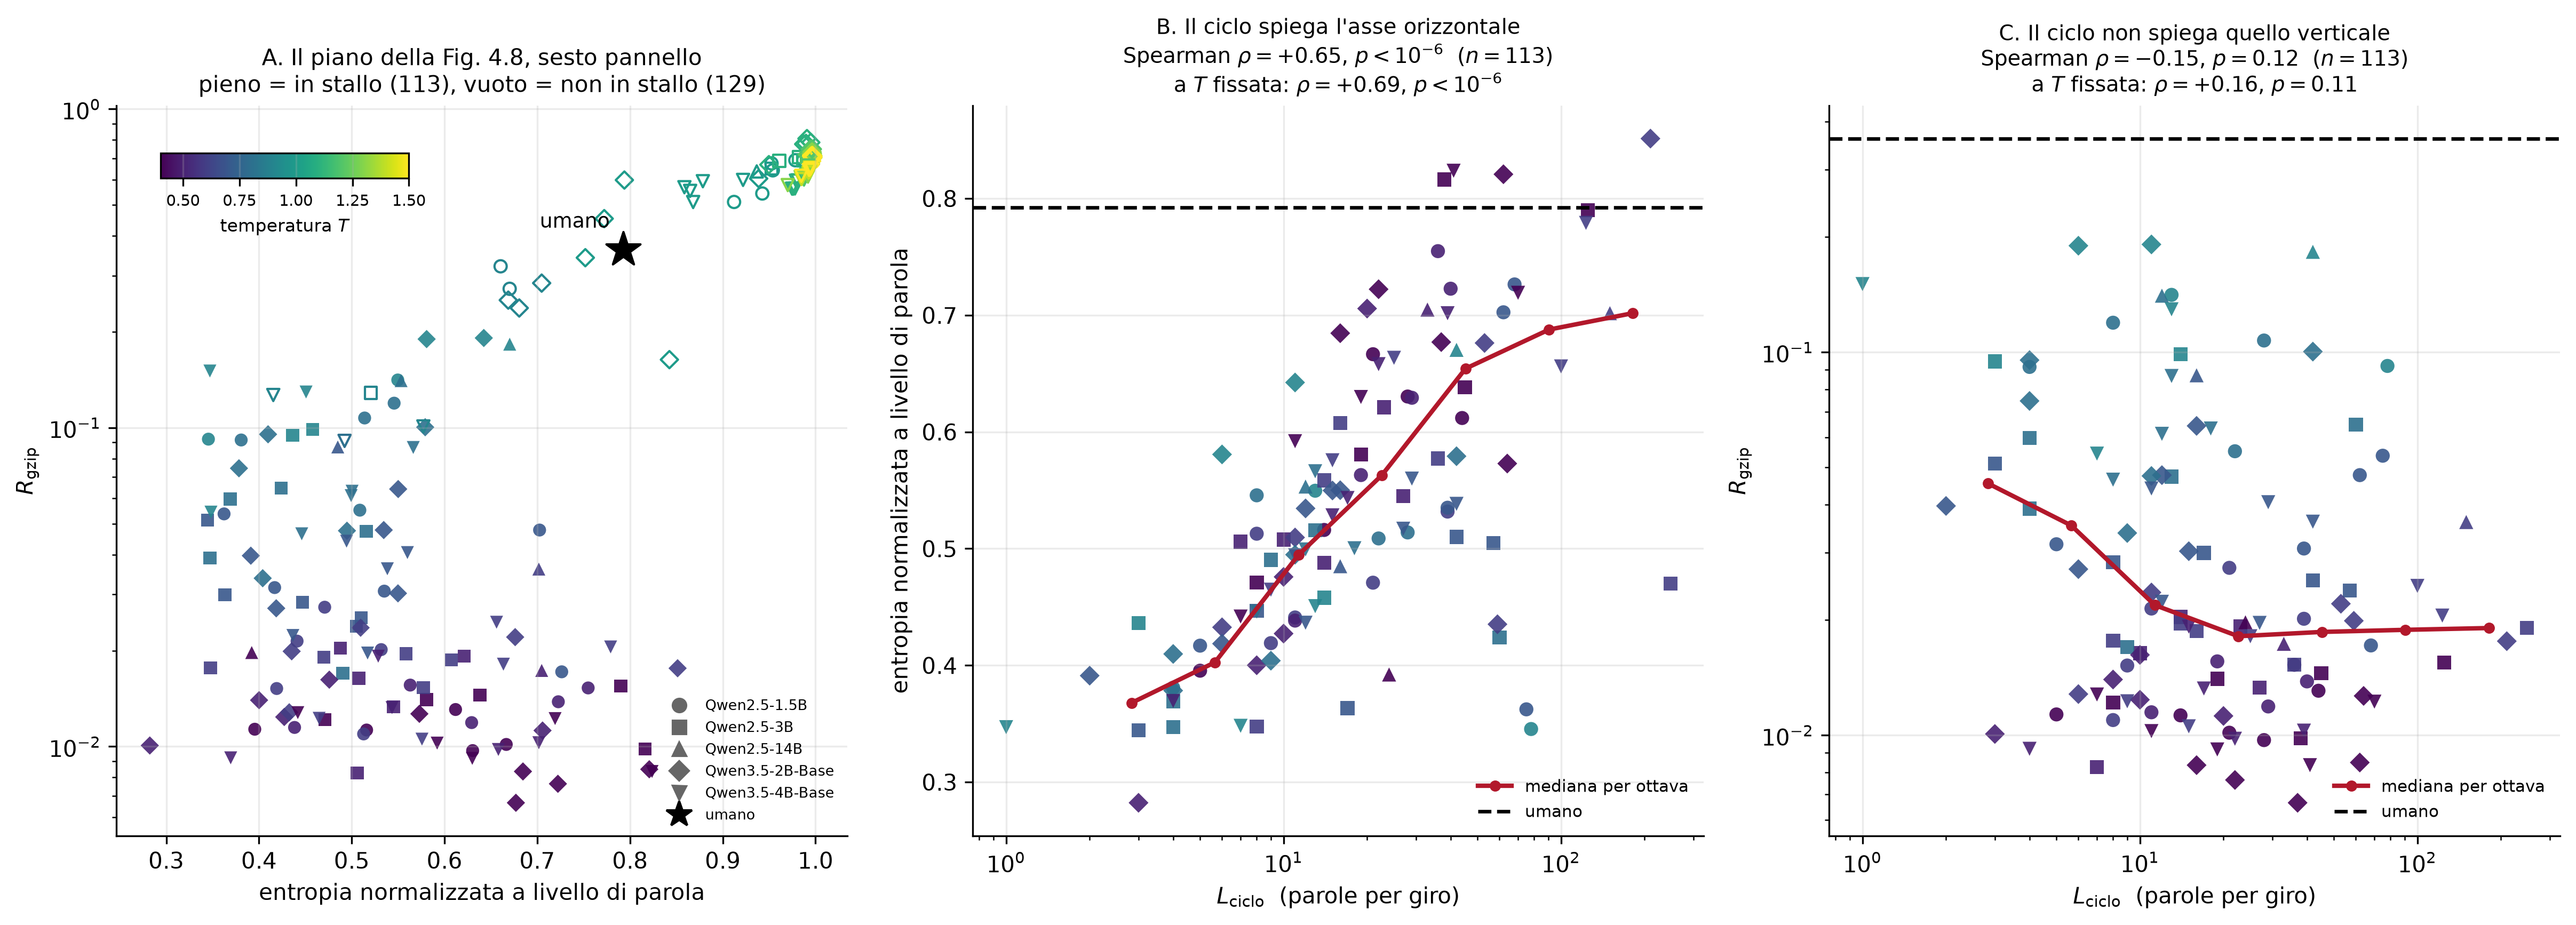
\includegraphics[width=\textwidth]{figure/cap4_ciclo_entropia.png}
  \caption{Lunghezza del ciclo ripetuto in fase di stallo. A: il piano
  entropia--comprimibilità della Figura~\ref{fig:compressione}, con i documenti
  in stallo a simbolo pieno e gli altri a simbolo vuoto; il colore codifica la
  temperatura e la forma il modello. B: entropia di parola contro lunghezza del
  ciclo, con la mediana per ottava. C: rapporto di compressione contro la stessa
  grandezza. La lunghezza del ciclo ordina l'asse orizzontale del piano e non
  quello verticale.}
  \label{fig:ciclo}
\end{figure}


% ---------------------------------------------------------------------
\section{Le tre fasi}
\label{sec:fasi-risultati}

Le misure precedenti descrivono il testo generato senza classificarlo. La regola
del §\ref{sec:tre-fasi} permette invece di assegnare ciascun documento a una
fase, e questa sezione ne riporta l'esito.

La traiettoria della~\eqref{eq:traiettoria} è costruita sui vettori GloVe a 100
dimensioni già impiegati nel §\ref{sec:token}, e l'autocorrelazione è calcolata
sui primi cento lag, misurati in parole. Il fit del GAPELMAPER usa invece un
intervallo più ampio, fino a 600 parole, perché distinguere una legge di potenza
da un esponenziale richiede più di una decade di distanze. Il livello di rumore
$\eta$ è stimato su una singola permutazione della traiettoria di ciascun
documento, con seme fissato.

Le due soglie della regola valgono $\kappa_{\min} = 0.50$ e $\Phi_{\min} = 3$.
La prima è deliberatamente permissiva: serve a escludere i documenti in cui meno
di metà delle parole ha un vettore, cioè quelli in cui la traiettoria è fatta per
lo più di zeri, e non a selezionare i documenti buoni. La seconda separa i due
gruppi in cui $\Phi$ effettivamente si distribuisce, e la sua posizione è poco
critica: come mostra la Figura~\ref{fig:transizioni}, fra la fase periodica e
quella successiva $\Phi$ cambia di due ordini di grandezza, cosicché qualunque
soglia compresa fra $1$ e $5$ produce la stessa classificazione. Il
§\ref{sec:tstar} riprende il punto trattando la fine della fase periodica come
uno degli otto criteri di temperatura critica.

La Figura~\ref{fig:acf} mostra come questa autocorrelazione cambia lungo lo
sweep. Fino a $T = 0.9$ la curva oscilla con periodo definito e ampiezza
prossima all'unità: il testo ripete un ciclo di parole, e a distanza pari a un
multiplo del ciclo ogni vettore ritrova sé stesso. Il periodo si accorcia al
crescere della temperatura, da dieci parole a $T = 0.5$ a circa tre a $T =
0.8$, mentre l'ampiezza scende da $0.98$ a $0.72$. Fra $T = 0.9$ e $T = 1.0$
la struttura periodica scompare del tutto: l'ampiezza cade a $0.036$ e la
curva diventa un decadimento monotono, senza più oscillazione. A $T = 1.3$
l'intera curva è contenuta nella banda di rumore stimata mescolando le parole
del documento, cioè non è distinguibile dal caso.

Il confronto con il testo umano chiarisce quanto entrambi i regimi siano
lontani dal linguaggio naturale. L'autocorrelazione del romanzo non è
periodica, con $\max\lvert\mathrm{FFT}\rvert$ pari a $1.16$, ben sotto la
soglia $3$, ma è nettamente sopra il livello di rumore su tutti i cento lag
esaminati, e il suo spettro decade in modo regolare invece di essere piatto.
Nessuna delle temperature campionate riproduce questa combinazione: sotto la
transizione la correlazione è troppo forte e periodica, sopra è assente.

\begin{figure}[htbp]
  \centering
  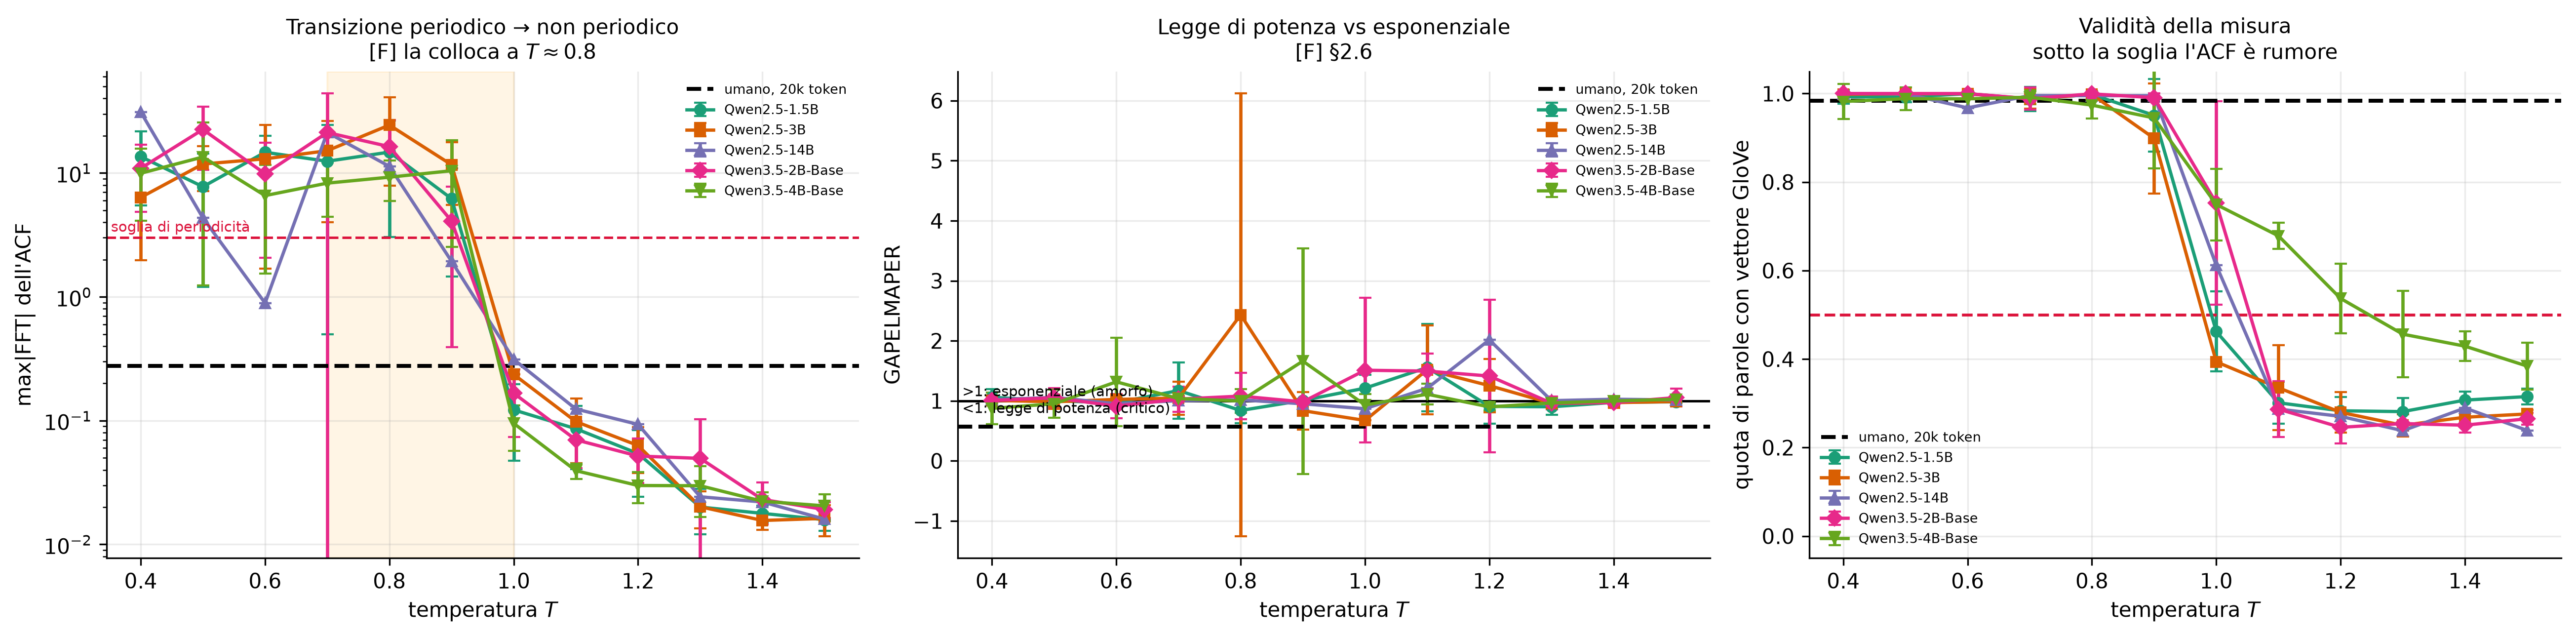
\includegraphics[width=\textwidth]{figure/cap4_transizioni_fase.png}
  \caption{Parametro di periodicità, GAPELMAPER e copertura degli embedding in
  funzione della temperatura. Il primo pannello è in scala logaritmica. Il terzo
  riporta la quota di parole dotate di un vettore, che è la condizione di
  validità delle altre due misure.}
  \label{fig:transizioni}
\end{figure}

\begin{figure}[htbp]
  \centering
  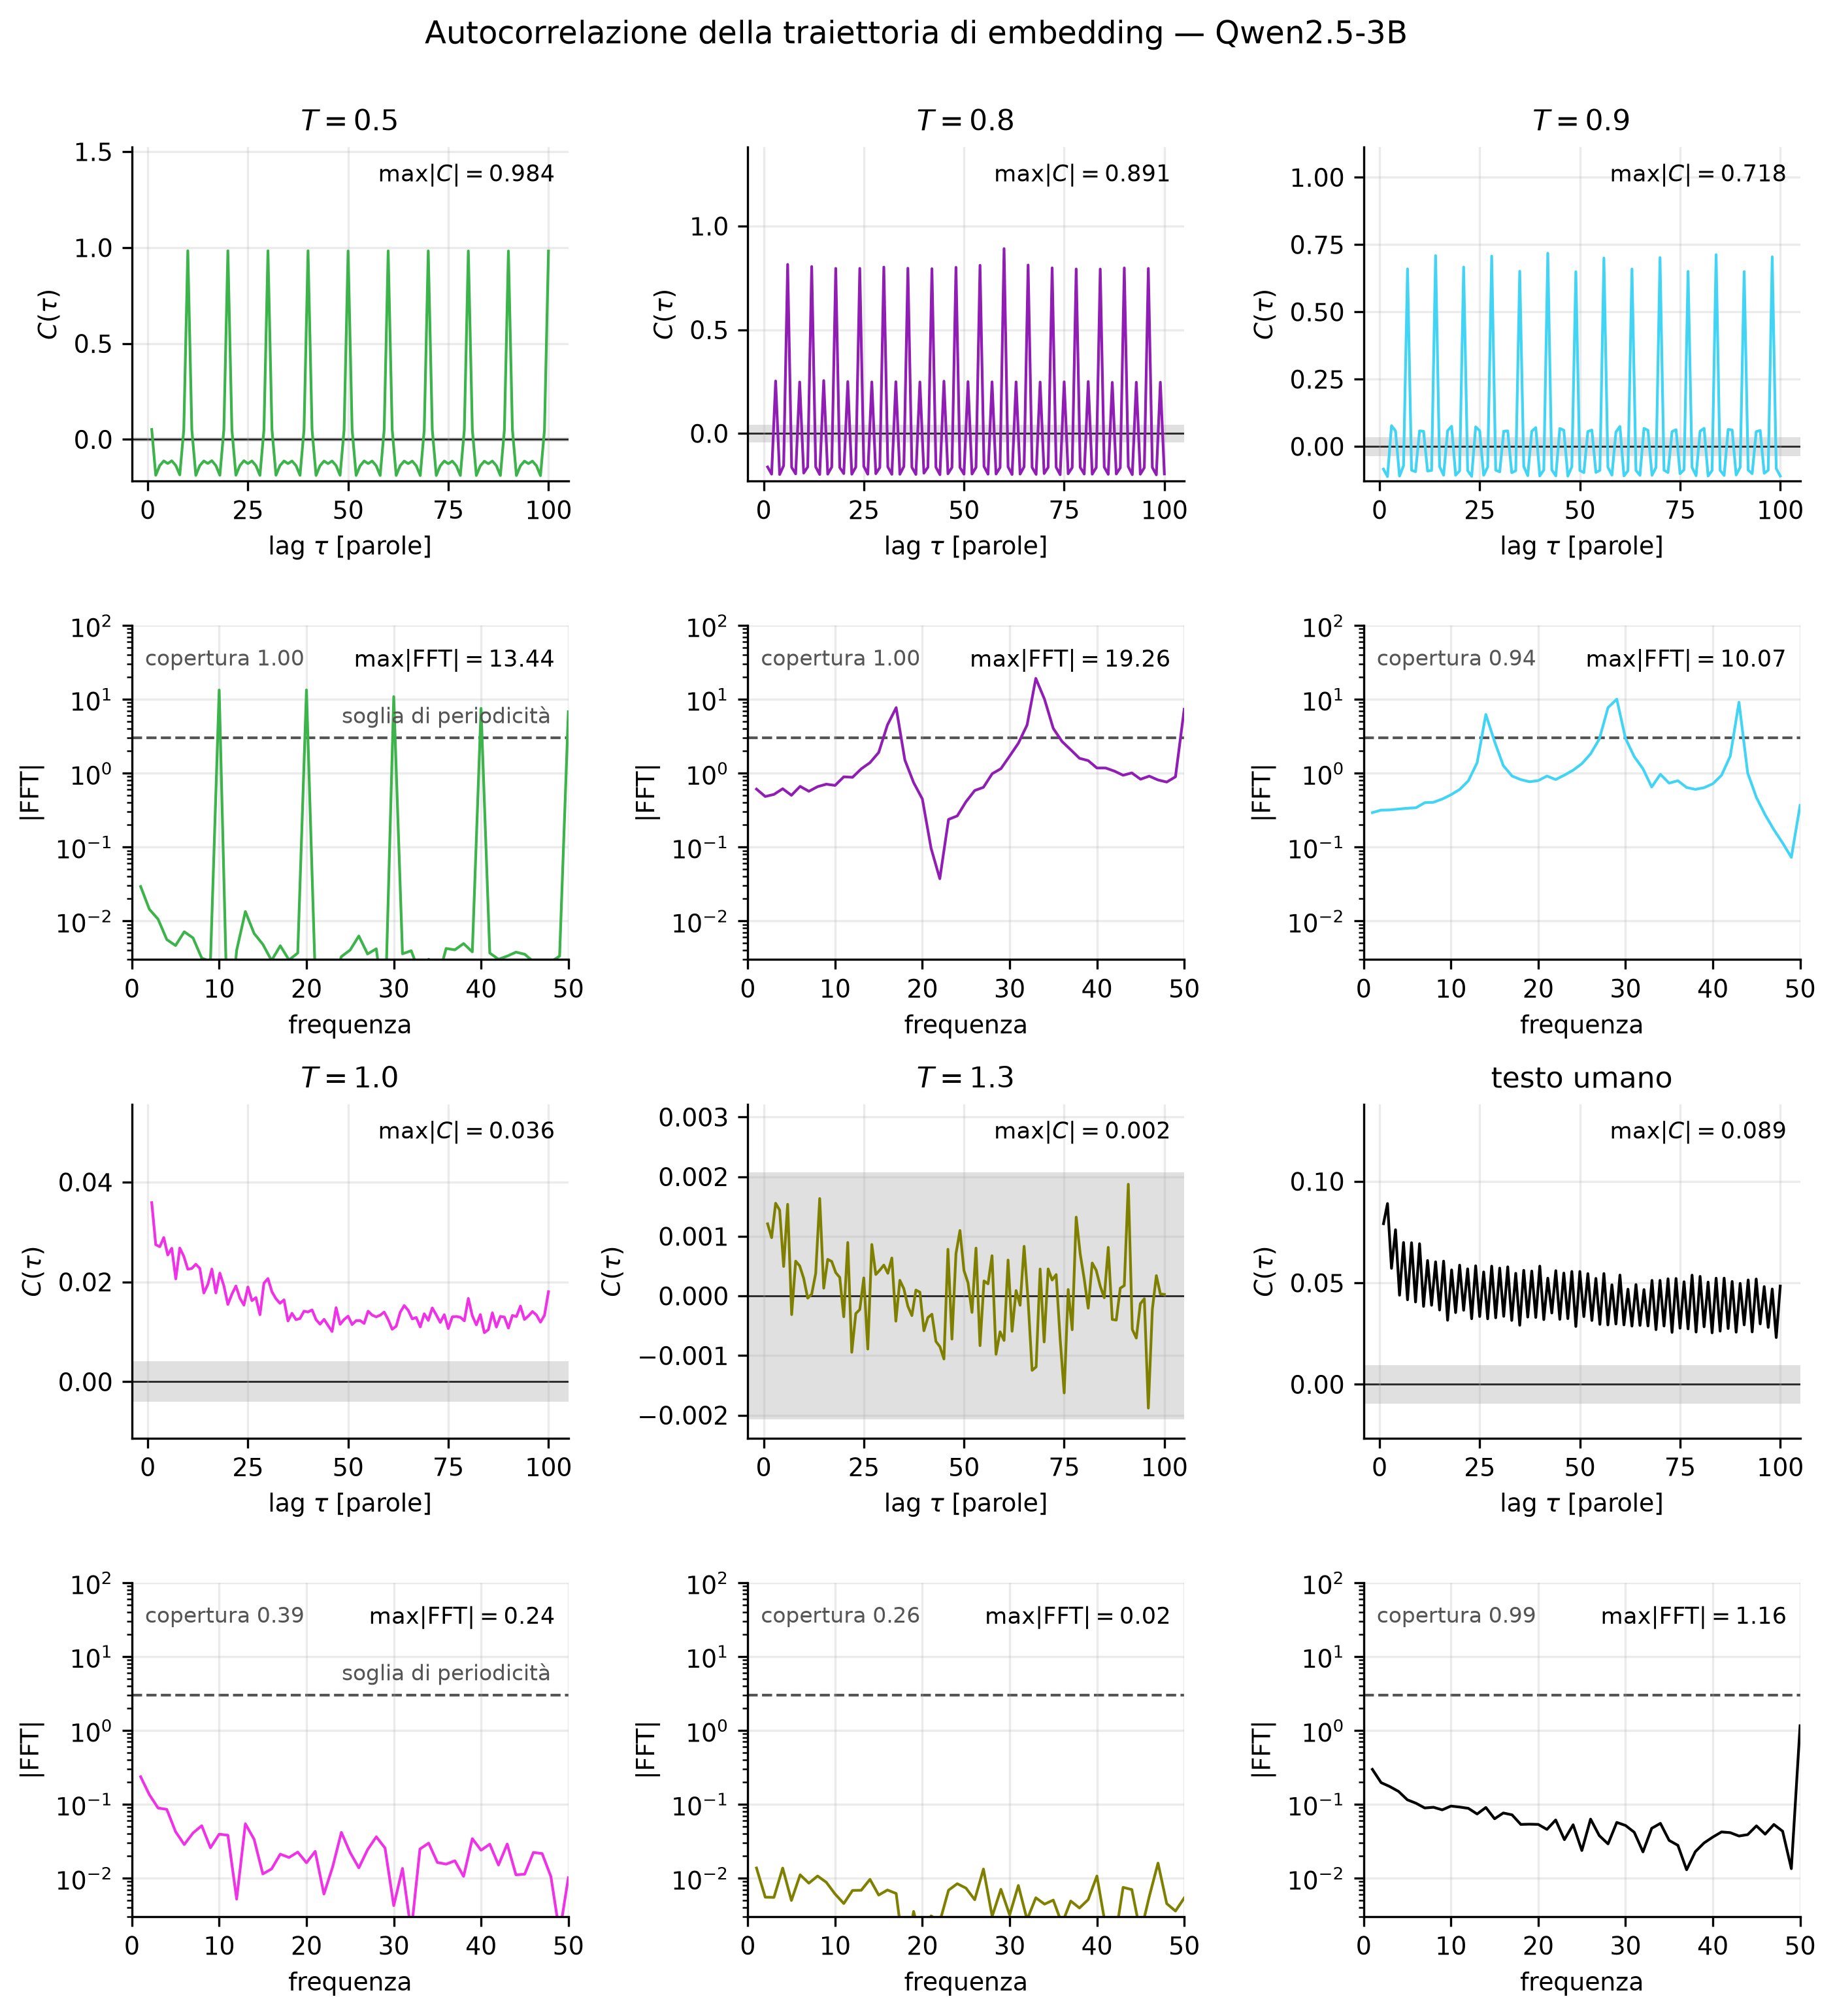
\includegraphics[width=\textwidth]{figure/cap4_acf_Qwen25_3B.png}
  \caption{Autocorrelazione della traiettoria di embedding per il modello
  Qwen2.5-3B a cinque temperature e sul testo umano di riferimento. In ciascuna
  coppia di riquadri il primo riporta $C(\tau)$ per lag da 1 a 100 parole e il
  secondo il modulo della sua trasformata di Fourier. La banda grigia è il
  livello di rumore, stimato ricalcolando $C(\tau)$ dopo aver permutato a caso
  le parole dello stesso documento; la linea tratteggiata è la soglia
  $\max\lvert\mathrm{FFT}\rvert = 3$ che separa la fase periodica. Per ogni
  temperatura è mostrato il campione di periodicità mediana, non il più marcato.
  La scala verticale di $C(\tau)$ è propria di ciascun riquadro, perché
  l'ampiezza varia di oltre due ordini di grandezza fra le temperature basse e
  quelle alte; il valore di picco è riportato dentro il riquadro. La scala dello
  spettro è invece logaritmica e comune, così i sei casi si confrontano
  direttamente.}
  \label{fig:acf}
\end{figure}

Il parametro d'ordine della prima transizione è il massimo modulo della
trasformata oltre il primo coefficiente, e il suo crollo è il risultato più
netto dell'intero capitolo. La media su tutti i modelli vale $16.0$ a
$T = 0.8$, scende a $7.5$ a $T = 0.9$ e precipita a $0.145$ a $T = 1.0$: un
fattore cinquanta in un solo passo di temperatura, e cento rispetto al massimo
di $T = 0.8$. Prosegue poi fino a $0.018$ a
$T = 1.5$, complessivamente tre ordini di grandezza sotto il massimo. Le cinque
curve dei diversi modelli si sovrappongono quasi esattamente, come mostra la
Figura~\ref{fig:transizioni}.

Anche questa soglia va confrontata con la fonte.
In~\cite{mikhaylovskiy2025states} la transizione dalla fase periodica è
collocata attorno a $t = 0.8$, con il testo dichiarato già non periodico a
$t = 1$, mentre qui la periodicità sopravvive fino a $T = 0.9$ e scompare a
$T = 1.0$. Lo spostamento verso l'alto è coerente con l'effetto del prompt
descritto nel §\ref{sec:protocollo}, che ritarda la comparsa delle proprietà
del regime disordinato.

\paragraph{Il secondo criterio non discrimina.} La distinzione fra stato
critico e fase amorfa dovrebbe essere operata dal GAPELMAPER, ma sui dati di
questo lavoro tale criterio non funziona. Il suo valore medio è $1.101$ con
deviazione standard $0.677$, e la quota di documenti con valore inferiore a 1,
cioè classificati come critici, è $0.51$: una moneta. Le barre d'errore nel
pannello centrale della Figura~\ref{fig:transizioni} sono di ampiezza
confrontabile con l'intero intervallo di variazione.

La difficoltà non è propria di questi dati. Lo stesso
\cite{mikhaylovskiy2025states} riporta che sui testi Qwen il GAPELMAPER è
raramente inferiore a 1, e che a diverse temperature del suo sweep non è
calcolabile affatto perché l'autocorrelazione assume valori negativi. Il
criterio, insomma, discrimina male anche nel lavoro che lo introduce.

Il motivo emerge dal terzo pannello. La copertura degli embedding resta sopra il
$95\%$ fino a $T = 0.9$, ma crolla a $0.64$ a $T = 1.0$ e a circa $0.31$ oltre
$T = 1.2$: nel regime in cui il GAPELMAPER dovrebbe distinguere le ultime due
fasi, l'autocorrelazione è calcolata su una minoranza delle parole e non
contiene più segnale. Per questa ragione i documenti che non superano la soglia
di copertura sono marcati come non valutabili anziché classificati, come
anticipato nel §\ref{sec:tre-fasi}. Senza tale precauzione il criterio avrebbe
assegnato una fase a documenti in cui non c'è nulla da misurare.

\paragraph{Il diagramma di fase.}
La Figura~\ref{fig:diagramma} riporta la composizione delle fasi per modello e
temperatura. Il quadro è coerente su tutti e cinque: fase periodica fino a
$T = 0.9$, dove la classificazione è ancora periodica per 13 documenti su 18;
scomparsa completa della periodicità a $T = 1.0$; documenti prevalentemente non
valutabili da $T = 1.1$ in poi, e completamente tali a $T \ge 1.4$.

\begin{figure}[htbp]
  \centering
  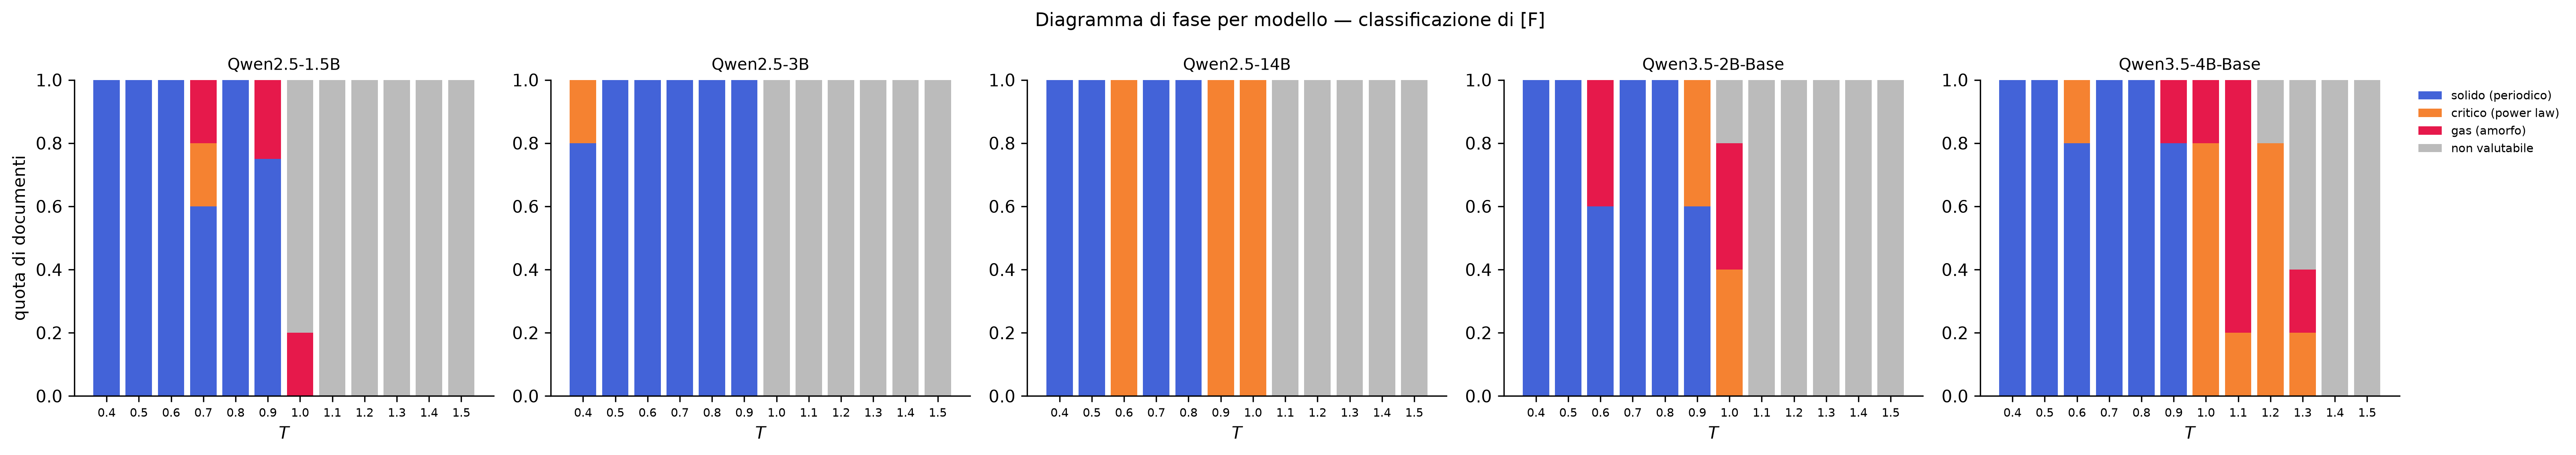
\includegraphics[width=\textwidth]{figure/cap4_diagramma_fase.png}
  \caption{Composizione delle fasi per modello e temperatura. La categoria «non
  valutabile» raccoglie i documenti che non superano la soglia di copertura
  degli embedding.}
  \label{fig:diagramma}
\end{figure}

Le tre modalità di fallimento del §\ref{sec:fallimenti} trovano qui la loro
interpretazione. La degenerazione per ripetizione è la fase periodica; la
degenerazione dell'alfabeto e del lessico corrisponde alla regione in cui la
misura non è più applicabile, che è a sua volta il segnale della fase amorfa. Il
testo non degenerato esiste solo nella striscia sottile fra le due, ed è la
stessa striscia in cui tutte le misure delle sezioni precedenti si avvicinano ai
valori umani.

% ---------------------------------------------------------------------
\section{Convergenza della temperatura critica}
\label{sec:tstar}

Le sezioni precedenti individuano ciascuna una temperatura privilegiata. Poiché
i criteri provengono da lavori indipendenti e misurano proprietà diverse del
testo, il loro accordo o disaccordo è esso stesso un risultato.

La Tabella~\ref{tab:tstar} riporta la temperatura selezionata da ciascun
criterio per ciascun modello. Due criteri sono intrinseci, nel senso che
individuano un estremo della curva senza far riferimento al testo umano: il
minimo del MAPE e la fine della fase periodica. Gli altri sei selezionano la
temperatura alla quale la misura si avvicina di più alla baseline umana.

\begin{table}[htbp]
\centering
\small
\begin{tabular}{@{}lccccc@{}}
\toprule
Criterio & 1.5B & 3B & 14B & 3.5-2B & 3.5-4B \\
\midrule
MAPE minimo                                  & 0.9 & 0.9 & 0.7 & 0.9 & 0.9 \\
$D_s$ minima dal testo umano                 & 0.9 & 0.9 & 0.9 & 0.9 & 1.0 \\
Fine della fase periodica                    & 1.0 & 1.0 & 0.6 & 1.0 & 1.0 \\
$R_{\mathrm{gzip}}$ più vicino all'umano     & 0.9 & 1.0 & 0.9 & 1.0 & 1.0 \\
$\alpha$ più vicino all'umano                & 1.0 & 1.5 & 1.3 & 1.0 & 1.0 \\
$R$ più vicino all'umano                     & 1.0 & 1.1 & 1.1 & 1.1 & 1.0 \\
$\gamma_H$ più vicino all'umano              & 1.1 & 1.0 & 1.3 & 1.1 & 1.3 \\
$\alpha_{\mathrm{DFA}}$ più vicino all'umano & 1.2 & 1.1 & 1.1 & 1.1 & 1.1 \\
\midrule
\textbf{mediana}                             & \textbf{1.0} & \textbf{1.0} &
\textbf{1.0} & \textbf{1.0} & \textbf{1.0} \\
\bottomrule
\end{tabular}
\caption{Temperatura selezionata da ciascun criterio, per ciascun modello. La
mediana vale $1.0$ per tutti e cinque i modelli, benché i singoli criteri
spazino da $0.6$ a $1.5$.}
\label{tab:tstar}
\end{table}

Il risultato principale del capitolo è la riga in fondo alla tabella. Otto
criteri tratti da quattro lavori indipendenti, costruiti per scopi diversi e mai
progettati per concordare, danno una mediana identica per tutti e cinque i
modelli. La convergenza non era scontata: i criteri misurano la distribuzione
delle frequenze, la crescita del vocabolario, le correlazioni a lungo raggio, la
comprimibilità e la periodicità dell'autocorrelazione, cioè proprietà che nulla
obbliga a coincidere.

\begin{figure}[htbp]
  \centering
  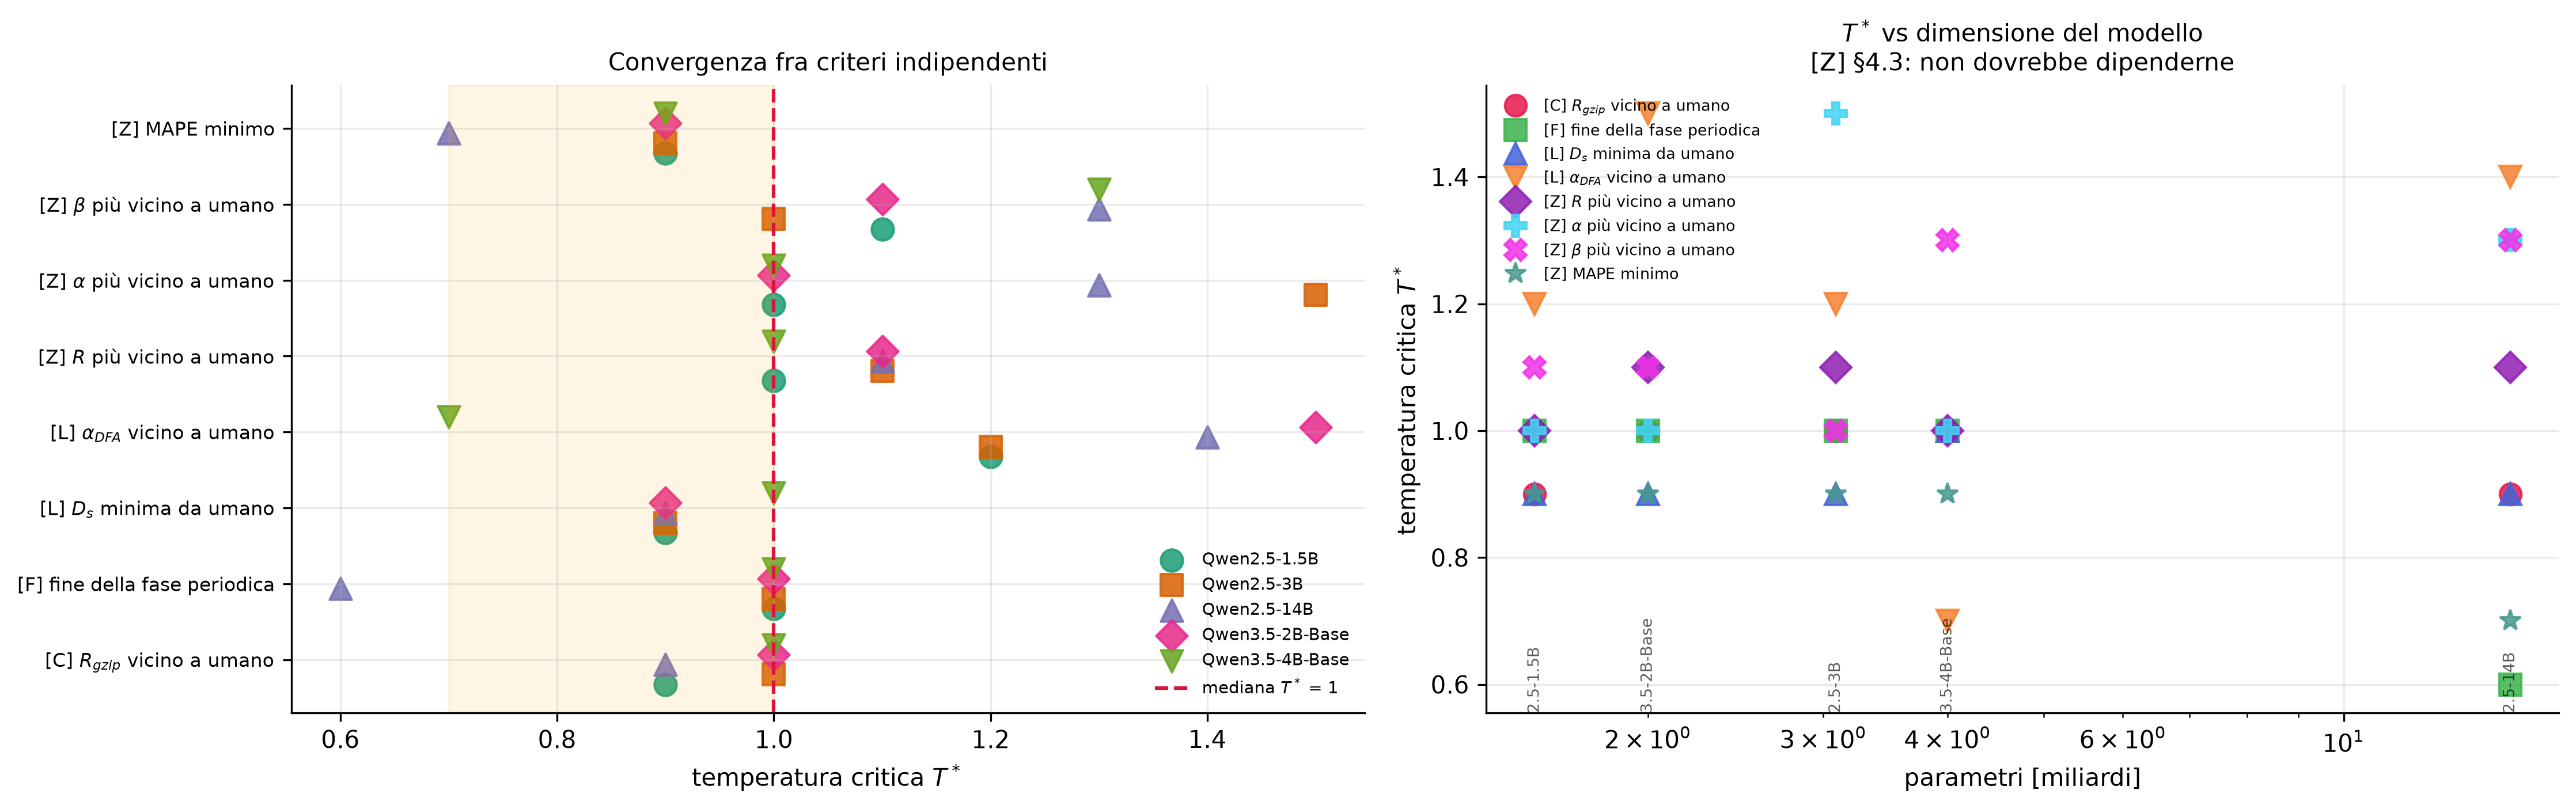
\includegraphics[width=\textwidth]{figure/cap4_temperatura_critica.png}
  \caption{A sinistra, la temperatura selezionata da ciascun criterio; la linea
  tratteggiata è la mediana complessiva e la banda la regione fra $0.7$ e $1.0$.
  A destra, la stessa quantità in funzione del numero di parametri del modello.}
  \label{fig:tstar}
\end{figure}

\paragraph{Dipendenza dalla dimensione del modello.}
La Figura~\ref{fig:tstar} riporta a destra la temperatura critica in funzione
del numero di parametri. La correlazione di rango è $\rho = -0.01$ con
$p = 0.93$ su quaranta osservazioni: nessuna dipendenza rilevabile. Il dato è
coerente con quanto riportato in~\cite{mikhaylovskiy2025zipf}, dove la posizione
dell'ottimo risulta indipendente dalla dimensione per tutte le famiglie
esaminate.

Un'assenza di correlazione misurata su cinque modelli appartenenti a due
famiglie non dimostra l'indipendenza: dimostra che, entro l'intervallo di
dimensioni esplorato e con la potenza statistica disponibile, non emerge
alcuna dipendenza. È coerenza con la letteratura, non conferma indipendente.

\paragraph{Una discordanza fra criteri.}
Due criteri si collocano sistematicamente fuori dal gruppo, e la loro distanza
dagli altri è essa stessa un risultato: mediarli insieme al resto la
cancellerebbe.

Il minimo del MAPE cade a $0.9$, mentre la fine della fase periodica cade a
$1.0$: alla temperatura in cui la distribuzione delle frequenze è più vicina a
una legge di potenza, l'autocorrelazione è ancora periodica per la maggioranza
dei documenti. Le due misure non si contraddicono, perché guardano oggetti
diversi, la statistica dei conteggi l'una e la struttura sequenziale l'altra,
e la loro distanza quantifica il fatto che le due proprietà non compaiono
simultaneamente. Il testo acquista una distribuzione di frequenze verosimile
prima di perdere la ripetizione.

Il criterio basato su $\alpha_{\mathrm{DFA}}$ merita una nota, perché il suo
esito dipende dall'ordine del detrending. Con il grado 1 seleziona temperature
fra $0.7$ e $1.5$, il più disperso dei nove; con il grado 2, che è quello
adottato qui per la ragione data nel §\ref{sec:robustezza}, si allinea agli
altri e sceglie $1.1$ per quattro modelli su cinque. La mediana per modello vale
$1.0$ in entrambi i casi. Resta valida l'avvertenza del
§\ref{sec:dfa-risultati}: alle basse temperature quell'esponente è instabile
fra documenti, e viene riportato per completezza anziché usato come criterio a
sé stante.

Una divergenza analoga fra criteri è documentata
in~\cite{mikhaylovskiy2025zipf} per i modelli Llama di grandi dimensioni, dove
le leggi di Zipf e di Heaps individuano temperature critiche sensibilmente
diverse. Il fenomeno non sembra dunque un artefatto di questo lavoro.

% ---------------------------------------------------------------------
\section{Che cosa lo sweep ha stabilito}
\label{sec:sintesi-cap4}

Tre risultati emergono dalle sezioni precedenti, di natura diversa fra loro.

Il primo è l'esistenza di una temperatura privilegiata, e la sua posizione. Otto
criteri costruiti per scopi diversi e tratti da quattro lavori indipendenti
danno una mediana identica, $T = 1.0$, per tutti e cinque i modelli, senza
dipendenza rilevabile dalla dimensione. Il secondo è che l'ottimo è stretto: la
transizione si consuma quasi interamente fra $T = 0.9$ e $T = 1.0$, dove il
parametro di periodicità cade di un fattore cinquanta, l'entropia passa da
$0.332$ a $5.77$ bit per carattere e il rapporto di compressione da $0.107$ a
$0.650$. Uno sweep a passo $0.1$ è appena sufficiente a risolvere quella
finestra.

Il terzo è l'esito negativo su cui poggia il capitolo successivo. L'esistenza
dell'ottimo è un fatto generale, ma la sua \emph{qualità} non lo è: due modelli
su cinque portano il MAPE al livello del testo umano e gli altri no. La
compressione condizionata non raggiunge il valore umano a nessuna temperatura,
ma per una ragione che non riguarda la struttura semantica: sotto la transizione
il testo ripete un ciclo e la seconda metà è prevedibile per costruzione, sopra
non è più linguaggio e non è prevedibile da nulla. Soprattutto, i documenti che
superano tutte e tre le soglie di non
degenerazione sono due su \num{242}. Il corpus generato lungo lo sweep non
sostiene quindi un'analisi semantica, ed è la ragione per cui il
Capitolo~\ref{cap:risultati2} cambia dominio anziché proseguire su questo.

Il capitolo non stabilisce però tutto. La convergenza dei criteri dice dove il
testo generato somiglia di più a quello umano secondo misure che ignorano il
significato; non dice se in quel punto il testo sia organizzato attorno a un
contenuto. È la domanda posta nel §\ref{sec:intro-domanda}, e richiede gli
strumenti del §\ref{sec:burst}.
%  Figure del corpo: modello Qwen2.5-3B. Quelle degli altri quattro
%  modelli stanno nel repository indicato in Appendice A.
% =====================================================================

\chapter{Il testo generato lungo lo sweep di temperatura}
\label{cap:risultati1}

Questo capitolo applica ai \num{242} documenti generati le misure introdotte nel
Capitolo~\ref{cap:teoria}, facendo variare la sola temperatura di campionamento.
Ogni misura viene confrontata con la baseline umana della
Tabella~\ref{tab:baseline}, calcolata con le stesse procedure e alla stessa
lunghezza.

Le figure del corpo del capitolo mostrano il modello Qwen2.5-3B, scelto come
esemplare perché dispone di cinque campioni per quasi tutte le temperature e
presenta le curve meno rumorose; le corrispondenti figure per gli altri quattro
modelli sono depositate nel repository indicato
nell'Appendice~\ref{app:codice}. Le curve aggregate
riportano invece tutti e cinque i modelli.

Il risultato principale non è nessuna delle singole misure, ma il fatto che
convergano: criteri tratti da quattro lavori indipendenti, costruiti per scopi
diversi, individuano la stessa regione di temperature. Il §\ref{sec:tstar} lo
documenta.

% ---------------------------------------------------------------------
\section{Le tre modalità di fallimento}
\label{sec:fallimenti}

La prima e la terza riga della Tabella~\ref{tab:tre-regimi} sono entrambe
prodotte dai modelli qui analizzati, a due temperature diverse, e mostrano i
due modi in cui la generazione si allontana dal linguaggio: la ripetizione letterale a bassa
temperatura, l'incoerenza semantica ad alta temperatura. Salendo ancora si
incontra un terzo regime, in cui l'alfabeto stesso si disgrega e il testo diventa
un miscuglio di sistemi di scrittura diversi.

Le tre modalità possono essere separate quantitativamente. Un documento viene
classificato come degenerato per \emph{ripetizione} se la quota di 8-grammi
ripetuti supera $0.10$, contro il valore $0.000$ misurato sul testo umano; come
degenerato nell'\emph{alfabeto} se la quota di caratteri non ASCII supera
$0.05$, più del triplo del valore umano $0.014$; come degenerato nel
\emph{lessico} se meno del $70\%$ delle sue parole possiede un vettore nello
spazio di embedding, contro il $98\%$ del testo umano. Le tre condizioni non si
escludono a vicenda, e un documento può soddisfarne più di una.

La Tabella~\ref{tab:fallimenti} riporta i conteggi.

\begin{table}[htbp]
\centering
\small
\begin{tabular}{@{}l>{\raggedright\arraybackslash}p{5.4cm}rr@{}}
\toprule
Modalità & Criterio & Documenti & Quota \\
\midrule
Ripetizione & 8-grammi ripetuti $> 0.10$      & 122 & 50\,\% \\
Alfabeto    & caratteri non ASCII $> 0.05$    & 125 & 52\,\% \\
Lessico     & copertura degli embedding $< 0.70$ & 112 & 46\,\% \\
\midrule
Nessuna     & prosa inglese non degenerata    &   2 &  1\,\% \\
\bottomrule
\end{tabular}
\caption{Modalità di degenerazione dei \num{242} documenti generati. Le
categorie non sono disgiunte. La classificazione dipende dalle soglie scelte,
ma non nella sostanza: facendole variare entro intervalli ragionevoli il numero
di documenti non degenerati resta compreso fra 2 e 7, cioè fra l'uno e il tre
per cento del totale.}
\label{tab:fallimenti}
\end{table}

Il dato va letto con attenzione, perché è il presupposto dell'intera seconda
parte sperimentale. Non significa che i modelli siano incapaci di produrre
linguaggio, ma che la finestra di temperature in cui lo producono è
sufficientemente stretta da non essere coperta da uno sweep a passo $0.1$: i
soli due documenti non degenerati compaiono a $T = 1.0$, e già a $T = 0.9$ e
$T = 1.1$ tutti i campioni ricadono in almeno una delle tre categorie. Il
Capitolo~\ref{cap:risultati2} muove da questa constatazione.


% ---------------------------------------------------------------------
\section{Legge di Zipf}
\label{sec:zipf-risultati}

La Figura~\ref{fig:zipf-cum} riporta gli istogrammi cumulativi delle frequenze,
una curva per temperatura, con la curva umana per confronto.

\begin{figure}[htbp]
  \centering
  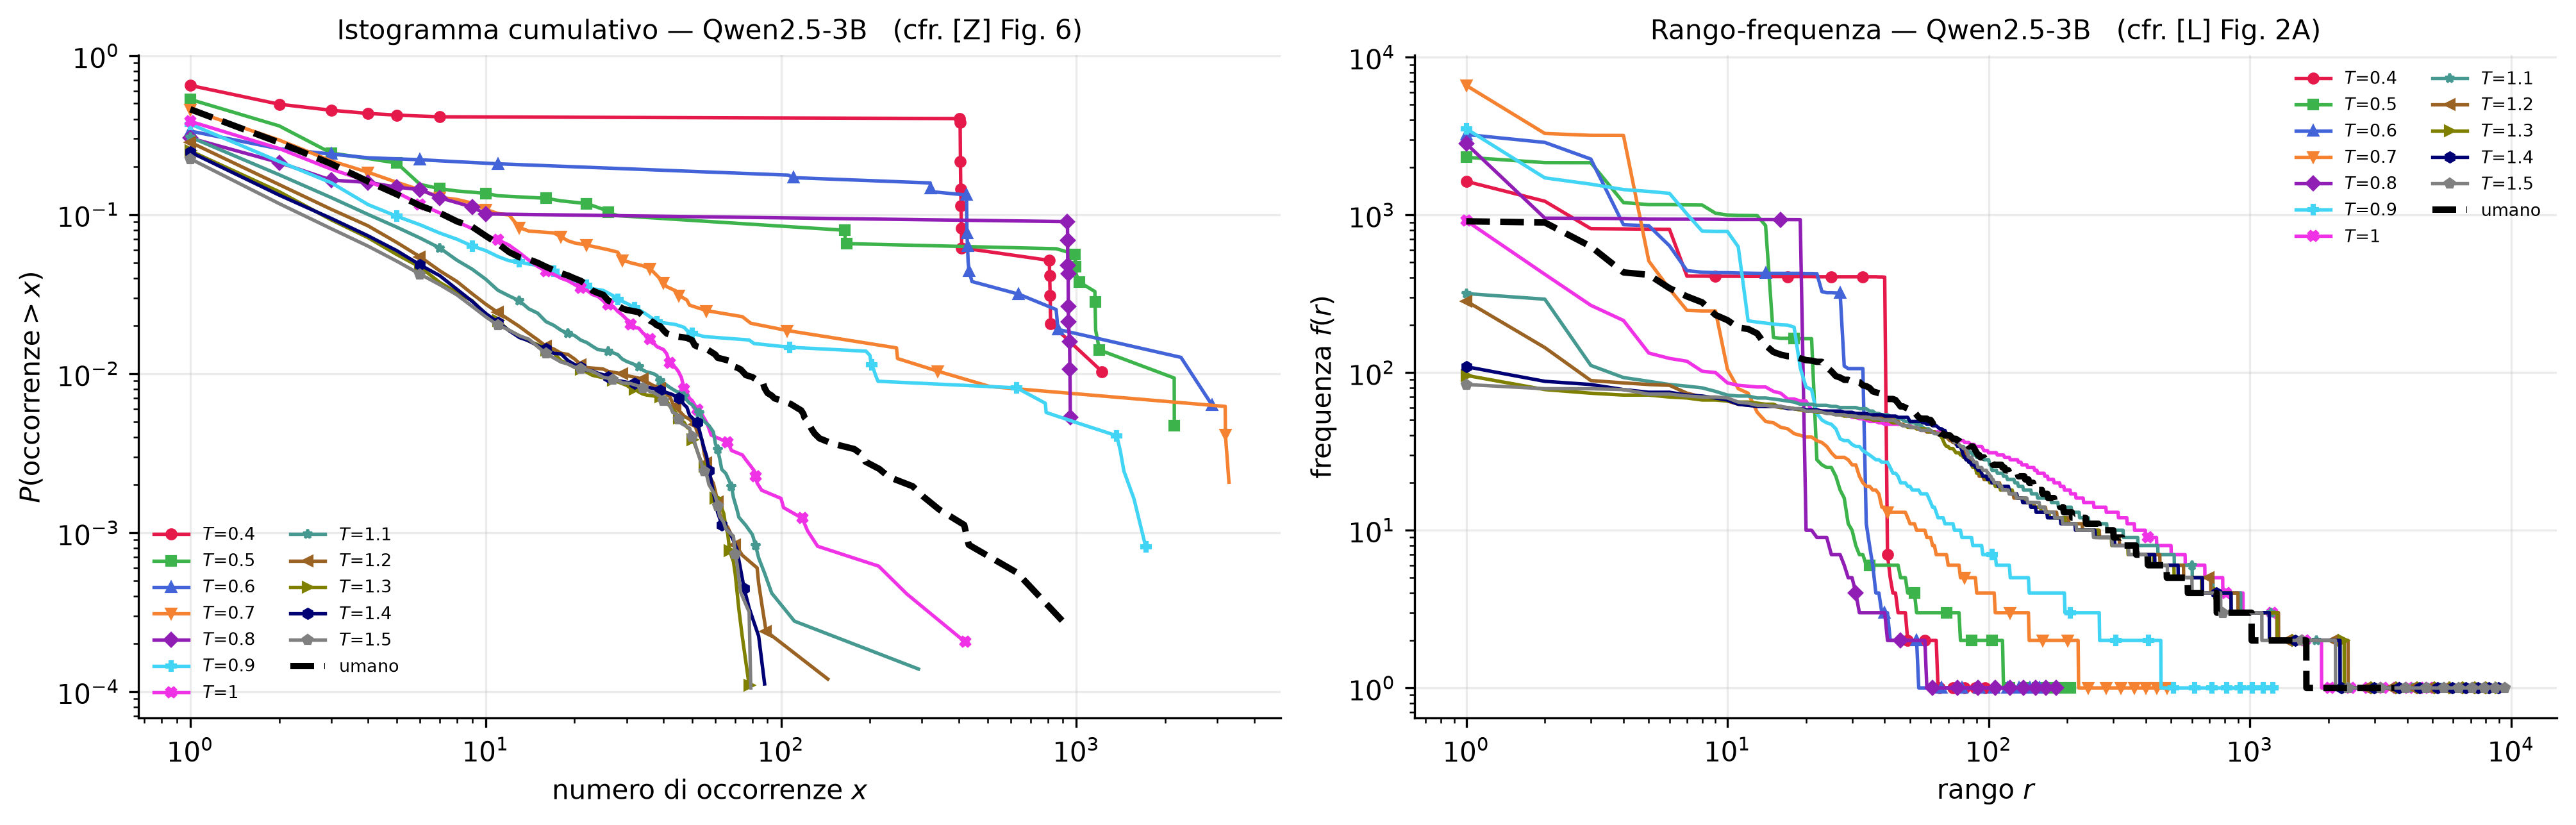
\includegraphics[width=\textwidth]{figure/cap4_zipf_cumulativo_Qwen25_3B.png}
  \caption{Istogrammi cumulativi delle frequenze dei token per il modello
  Qwen2.5-3B, una curva per temperatura. A bassa temperatura la curva è quasi
  verticale, perché pochi token coprono l'intero documento; ad alta temperatura
  è quasi orizzontale, perché quasi ogni token compare una volta sola. Solo
  nella regione intermedia la curva si avvicina alla retta che in coordinate
  bilogaritmiche corrisponde a una legge di potenza.}
  \label{fig:zipf-cum}
\end{figure}

L'esponente da solo non basta a descrivere questo comportamento, ed è la ragione
per cui nel §\ref{sec:zipf} è stato introdotto il MAPE: una curva può avere la
pendenza corretta e una curvatura marcata, e in tal caso l'esponente stimato non
descrive nulla. La Figura~\ref{fig:zipf-vs-T} riporta entrambe le quantità in
funzione della temperatura.

\begin{figure}[htbp]
  \centering
  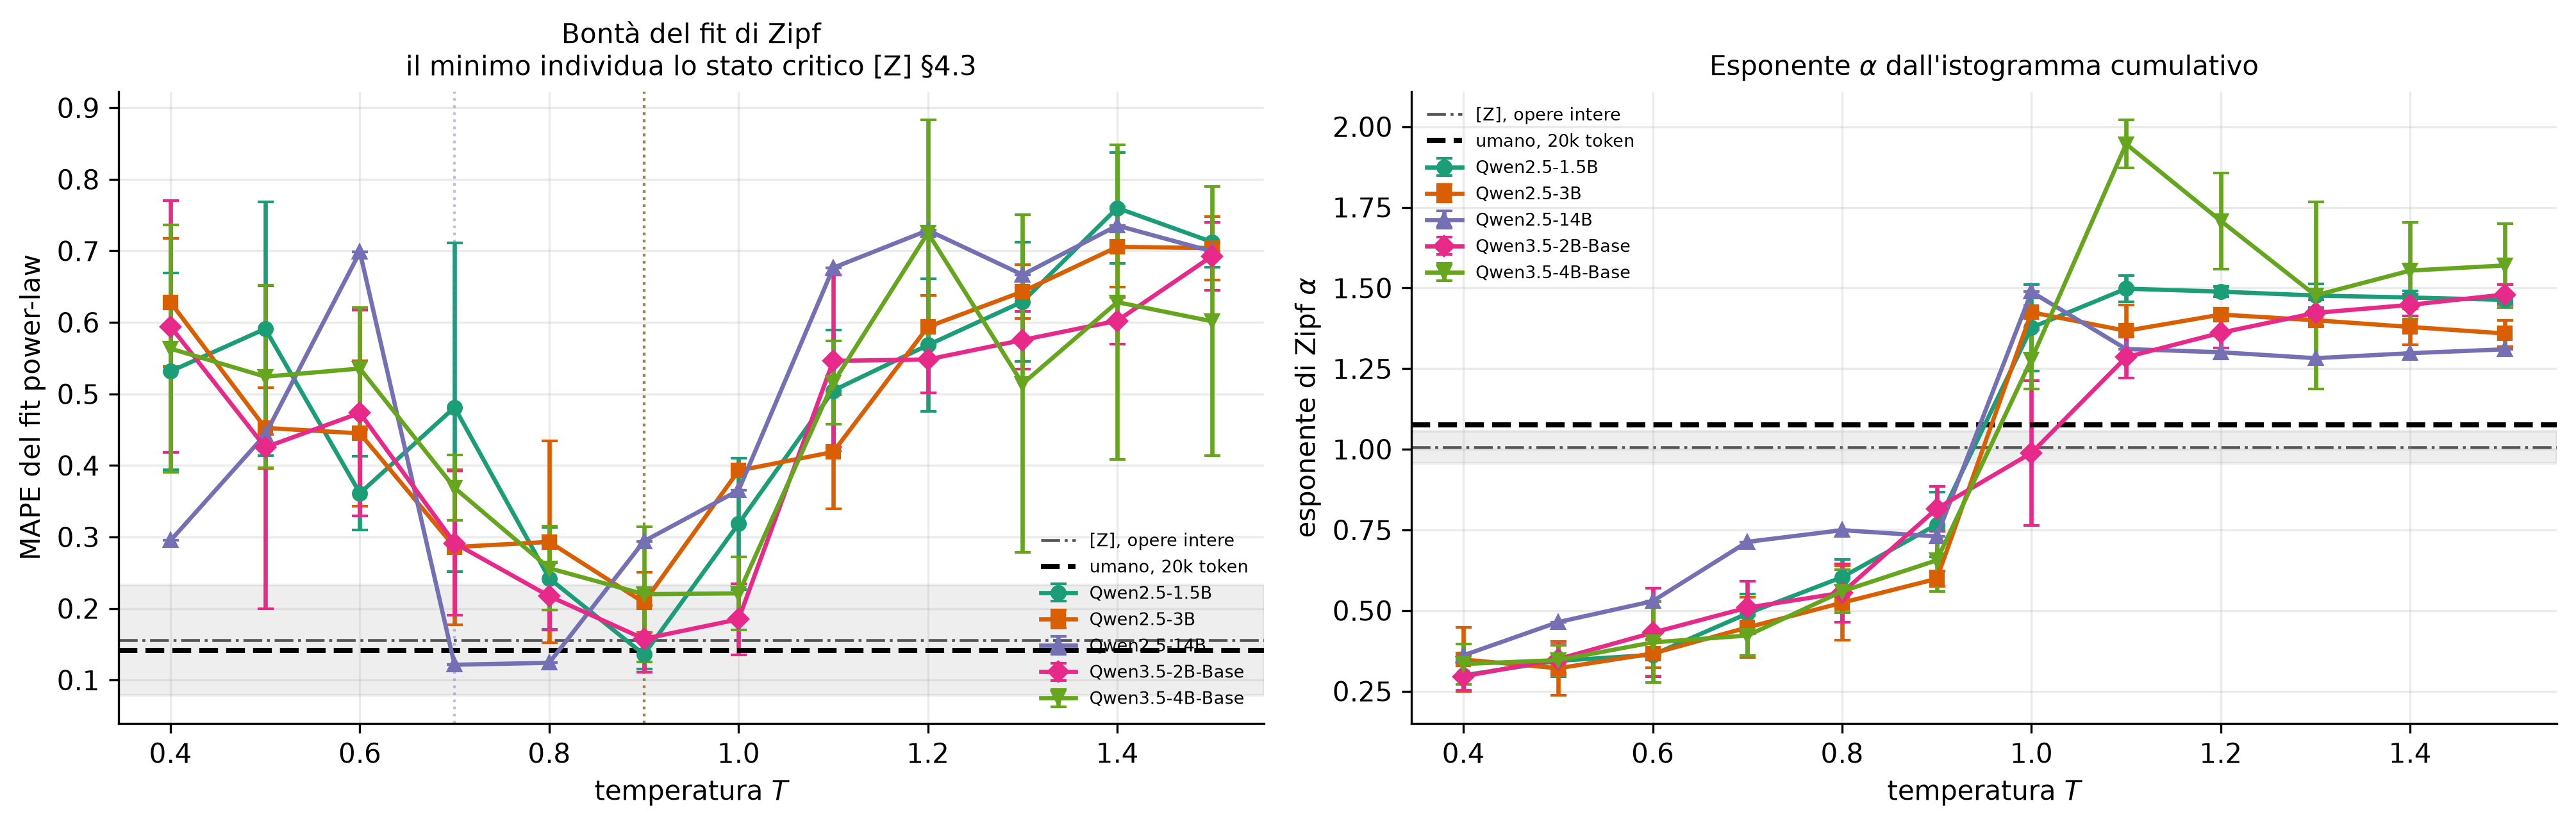
\includegraphics[width=\textwidth]{figure/cap4_zipf_vs_T.png}
  \caption{Bontà del fit e esponente della legge di Zipf in funzione della
  temperatura, per tutti e cinque i modelli. La banda grigia è il valore
  pubblicato su testi letterari interi, la linea nera tratteggiata la baseline
  umana misurata alla lunghezza di lavoro.}
  \label{fig:zipf-vs-T}
\end{figure}

Il MAPE ha un minimo pronunciato, che cade a $T = 0.9$ per quattro modelli su
cinque e a $T = 0.7$ per il modello da 14 miliardi di parametri. È il
risultato centrale della sezione: esiste una temperatura alla quale la
distribuzione delle frequenze del testo generato è più vicina a una legge di
potenza, e ai due lati di essa l'aderenza peggiora rapidamente.

Al minimo il MAPE del modello esemplare vale $0.208$. I due termini di
riferimento sono la baseline umana misurata alla stessa lunghezza, che vale
$0.141$, e il valore $0.156 \pm 0.077$ che~\cite{mikhaylovskiy2025zipf} riporta
su un corpus di sei opere letterarie in cinque lingue. Che i due riferimenti
umani cadano tanto vicini è una verifica indipendente della taratura della
baseline: sono ottenuti con tokenizzatori diversi, su testi diversi e di
lunghezza diversa, e la deriva documentata nella
Figura~\ref{fig:dimensione-finita} non rendeva scontato l'accordo.

Il valore del modello va letto contro tre metri diversi, e il giudizio che se ne
ricava non è lo stesso. Rispetto al modello stesso, $0.208$ è un risultato
netto: alle due estremità dell'intervallo lo stesso modello dà $0.628$ e
$0.704$, cioè un errore di fit tre volte più grande. Rispetto al testo umano è
invece una mezza vittoria: $0.208$ è circa una volta e mezza $0.141$, e resta
dentro la banda pubblicata solo perché quella banda è larga, sfiorandone il
margine superiore $0.233$. Rispetto agli altri modelli, infine, è un risultato
mediocre. La Tabella~\ref{tab:mape-minimi} riporta i cinque minimi: due modelli
scendono sotto il valore umano e un terzo vi si accosta, con $0.158$ contro
$0.141$, mentre il modello esemplare e il Qwen3.5-4B restano sopra.

\begin{table}[htbp]
\centering
\small
\begin{tabular}{@{}lrr@{}}
\toprule
Modello & $T$ del minimo & MAPE al minimo \\
\midrule
Qwen2.5-14B      & 0.7 & 0.121 \\
Qwen2.5-1.5B     & 0.9 & 0.136 \\
Qwen3.5-2B-Base  & 0.9 & 0.158 \\
Qwen2.5-3B       & 0.9 & 0.208 \\
Qwen3.5-4B-Base  & 0.9 & 0.220 \\
\midrule
testo umano      & --- & 0.141 \\
\bottomrule
\end{tabular}
\caption{Valore minimo del MAPE e temperatura alla quale viene raggiunto, per
ciascun modello, con la baseline umana misurata alla stessa lunghezza. Il
minimo esiste per tutti e cinque, ma solo tre modelli lo portano al livello del
testo umano o sotto. La riga del Qwen2.5-14B è ricavata da un solo campione per
temperatura e va letta con la cautela discussa nel testo.}
\label{tab:mape-minimi}
\end{table}

La prima riga della tabella richiede una precauzione. Il Qwen2.5-14B è l'unico
modello con un solo campione per temperatura, contro i tre o cinque degli altri,
e la sua curva del MAPE non è regolare da nessuno dei due lati del minimo: vale
$0.295$ a $T = 0.4$, sale a $0.698$ a $T = 0.6$ e scende a $0.121$ a $T = 0.7$,
cioè peggiora di un fattore due e migliora di un fattore sei in due passi
consecutivi. Negli altri quattro modelli la dispersione fra campioni alla stessa
temperatura va da $0.046$ a $0.230$ attorno a $T = 0.7$, mentre la distanza fra
il minimo del 14B e il suo valore a $T = 0.9$ vale $0.173$: sta dentro
quell'intervallo. Con una sola realizzazione la posizione del minimo non è
risolvibile, e il valore $T = 0.7$ va letto come compatibile con il $T = 0.9$
degli altri quattro anziché come uno spostamento reale. La stessa cautela vale
per la profondità: $0.121$ è il minimo più basso dei cinque ed è anche il meno
affidabile, mentre il $0.136$ del Qwen2.5-1.5B poggia su cinque campioni con
dispersione $0.020$ ed è l'unico caso in cui il primato sul testo umano è
sostenuto da repliche.

La posizione del minimo va confrontata con quella riportata nella fonte.
In~\cite{mikhaylovskiy2025zipf} il minimo del MAPE cade fra $t = 1.0$ e
$t = 1.2$ per tutti i modelli tranne i Llama più grandi, mentre qui cade a
$T = 0.9$ per quattro modelli su cinque. Lo scarto è nella direzione prevista
dall'effetto del prompt descritto nel §\ref{sec:protocollo}, che abbassa
l'errore del fit soprattutto alle basse temperature e sposta quindi il minimo
verso sinistra.

Ne segue una distinzione che vale per tutto il seguito. L'esistenza
di una temperatura ottimale è un fatto generale, comune a tutti e cinque i
modelli; la qualità dell'ottimo, cioè quanto il testo generato in quel punto
somigli davvero a un testo umano, varia da modello a modello e non è garantita.
Il modello scelto come esemplare non è fra quelli che ci riescono, e i grafici
del corpo del capitolo vanno letti tenendolo presente.

L'esponente $\alpha$ racconta la stessa storia da un'altra angolazione. Per il
modello esemplare passa da $0.35$ a $T = 0.4$, valore che corrisponde a una
distribuzione dominata da pochissimi tipi, a $1.36$ a $T = 1.5$, dove più di tre
quarti dei tipi compaiono una volta sola.\footnote{Un tipo che compare una sola
volta nel testo si dice \emph{hapax}. Gli hapax sono normalmente la maggioranza
dei tipi ma una piccola parte delle occorrenze: nella baseline umana usata qui
sono il $54\%$ dei tipi e il $10\%$ dei token, mentre a $T = 1.5$ il modello
esemplare arriva al $77\%$ dei tipi e al $37\%$ dei token.} La transizione non è
graduale: fra $T = 0.9$ e $T = 1.0$ l'esponente salta da $0.60$ a $1.43$,
attraversando in un solo passo il valore umano $1.076$, per poi assestarsi
attorno a $1.4$ senza più avvicinarvisi.

% ---------------------------------------------------------------------
\section{Legge di Heaps e descrittore \texorpdfstring{$R$}{R}}
\label{sec:heaps-risultati}

Le curve di crescita del vocabolario rendono immediatamente evidente perché il
§\ref{sec:heaps} abbia dovuto introdurre un descrittore alternativo all'esponente di
Heaps.

\begin{figure}[htbp]
  \centering
  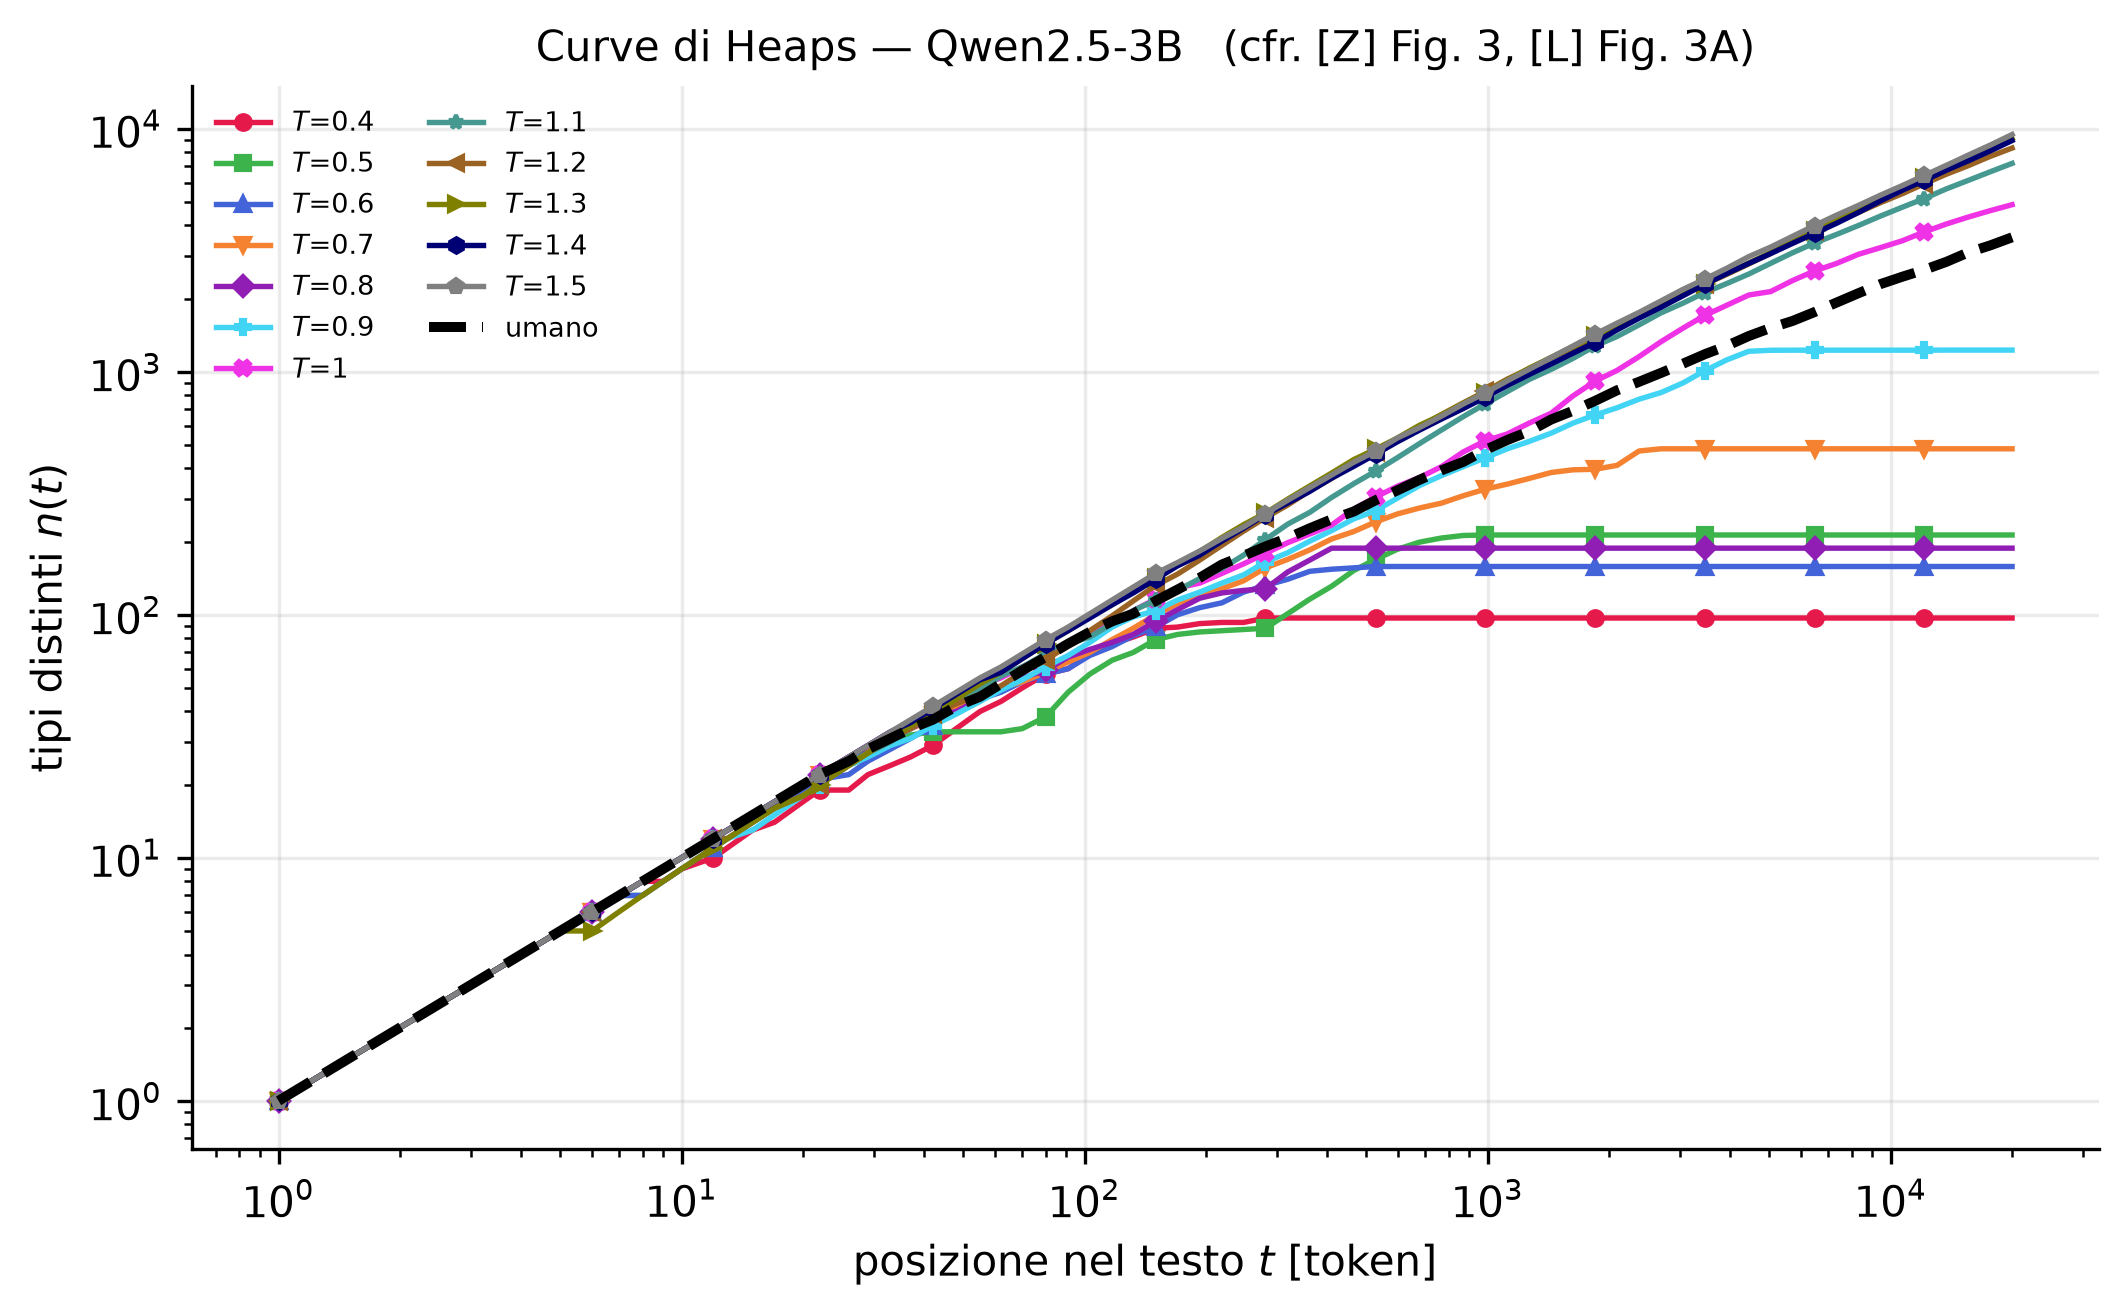
\includegraphics[width=0.86\textwidth]{figure/cap4_heaps_curve_Qwen25_3B.png}
  \caption{Crescita del vocabolario per il modello Qwen2.5-3B. Alle temperature
  basse la curva si appiattisce dopo poche migliaia di token: il modello ha
  smesso di produrre tipi nuovi. Alle temperature alte cresce quasi linearmente.
  In nessuno dei due casi la curva è una legge di potenza, e stimarne
  l'esponente restituisce un numero privo di contenuto.}
  \label{fig:heaps-curve}
\end{figure}

La Figura~\ref{fig:heaps-R} riporta il descrittore $R$, l'esponente $\gamma_H$
e il rapporto fra tipi e occorrenze in funzione della temperatura. I tre
andamenti sono concordi: per il modello esemplare $\gamma_H$ passa da $0.001$
a $T = 0.4$, dove la curva è piatta e il vocabolario non cresce affatto, a
$0.806$ a $T = 1.5$, attraversando il valore umano $0.668$ poco sopra $T =
0.9$. Il descrittore $R$ passa da $0.003$ a $0.688$ e incrocia il valore umano
$0.507$ attorno a $T = 1.05$.

Il terzo pannello riporta la quantità più elementare delle tre, il rapporto fra
il numero di tipi distinti e il numero di occorrenze, e serve da controllo sulle
altre due. A differenza di $\gamma_H$ e di $R$ non richiede alcun fit né alcuna
partizione del documento, quindi non può essere alterato da un modello mal
specificato: se le tre curve concordano, l'andamento non è un artefatto della
procedura di stima. Per il modello esemplare passa da $0.007$ a $T = 0.4$ a
$0.474$ a $T = 1.5$, e attraversa il valore umano $0.179$ fra $T = 0.9$ e
$T = 1.0$, cioè nello stesso punto delle altre due misure. Il pannello mostra
però anche in che senso l'accordo con il testo umano sia solo locale: sopra
$T = 1.1$ il rapporto supera il doppio del valore umano e continua a crescere,
mentre $\gamma_H$ resta stabile attorno a $0.8$. Le due misure smettono di dire
la stessa cosa non appena il vocabolario si allarga oltre quello di un romanzo.

\begin{figure}[htbp]
  \centering
  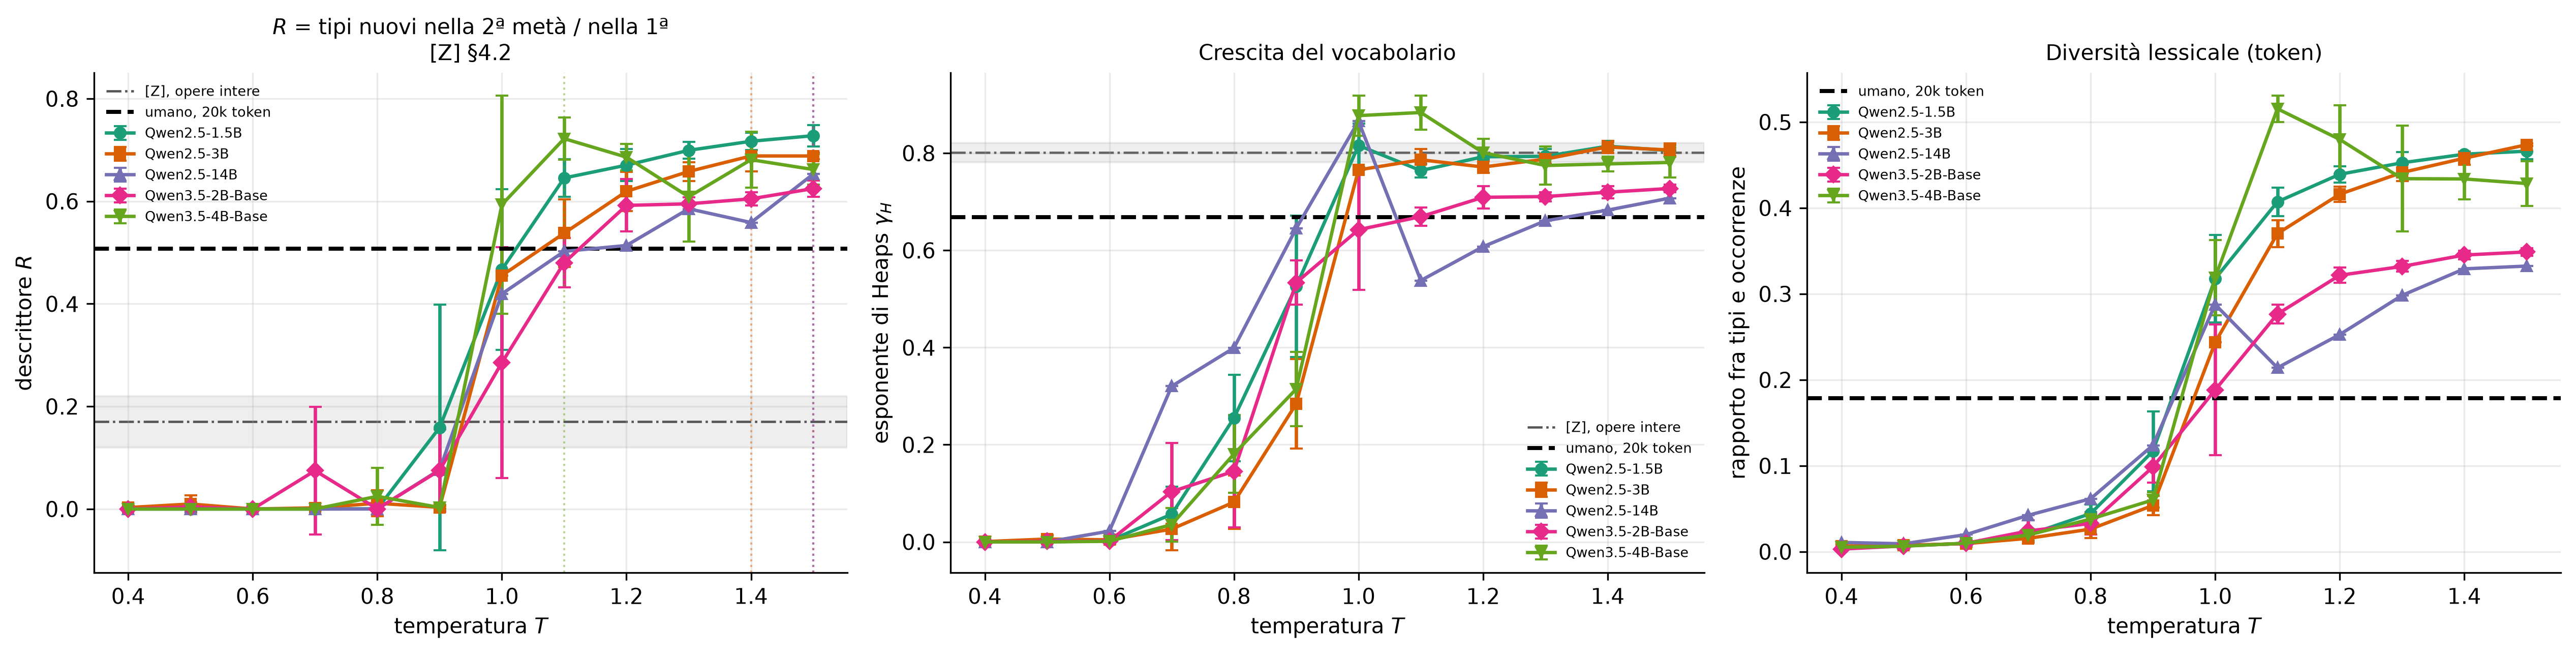
\includegraphics[width=\textwidth]{figure/cap4_heaps_R_vs_T.png}
  \caption{Descrittore $R$, esponente di Heaps e rapporto fra tipi e occorrenze
  in funzione della temperatura. La banda grigia riporta i valori pubblicati su
  opere intere, che per le ragioni discusse nel §\ref{sec:scelte} non sono un
  termine di confronto diretto.}
  \label{fig:heaps-R}
\end{figure}

% ---------------------------------------------------------------------
\section{Correlazioni a lungo raggio}
\label{sec:dfa-risultati}

Ogni documento viene convertito nella successione numerica definita nel
§\ref{sec:dfa}: ogni carattere è sostituito dal proprio rango di frequenza nel
documento, $1$ al più frequente, $2$ al secondo, e così via. È su quella
successione che si misura l'esponente della fluttuazione. Il detrending è
quadratico: il §\ref{sec:robustezza} documenta il confronto con quello lineare e
la ragione della scelta, cioè che alle basse temperature i documenti non sono
stazionari e un polinomio di primo grado non assorbe la deriva della
composizione dei caratteri. Il primo controllo riguarda il null model: la stessa
analisi condotta sui documenti rimescolati deve restituire un esponente pari a
$1/2$.


La Figura~\ref{fig:dfa} riporta le curve di fluttuazione e l'esponente in
funzione della temperatura. L'esponente ha un massimo a $T = 1.0$, dove vale
$0.719$ in media su tutti i modelli, superiore al valore umano di $0.579$;
decresce poi verso $0.53$ alle temperature più alte, avvicinandosi al valore del
rimescolamento senza raggiungerlo.

\begin{figure}[htbp]
  \centering
  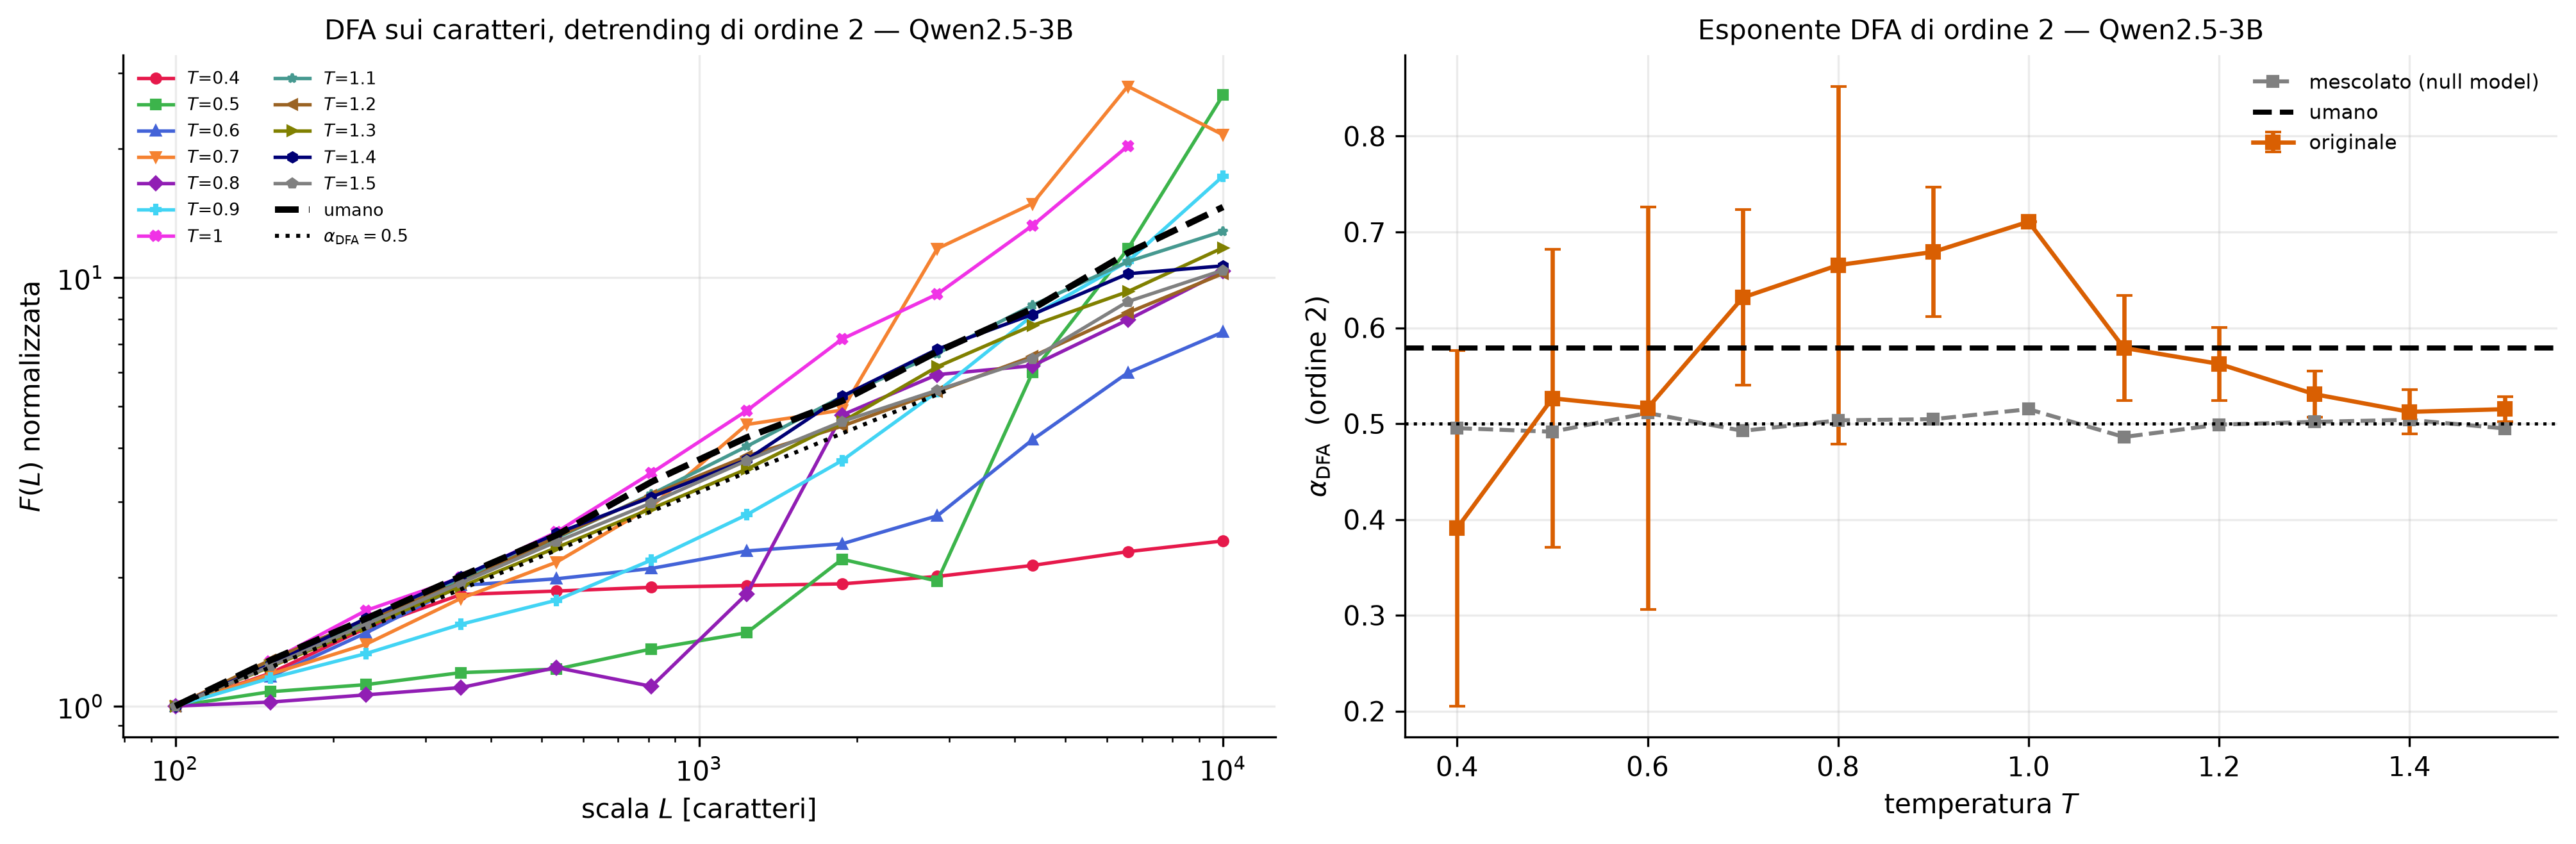
\includegraphics[width=\textwidth]{figure/cap4_dfa_Qwen25_3B_o2.png}
  \caption{Fluttuazione detrendizzata per il modello Qwen2.5-3B, con detrending
  quadratico. A sinistra $F(s)$ in funzione della scala, una curva per
  temperatura, con la pendenza di riferimento $\alpha_{\mathrm{DFA}} = 1/2$; a
  destra l'esponente in funzione della temperatura, con il null model
  rimescolato e la baseline umana.}
  \label{fig:dfa}
\end{figure}

\paragraph{La dispersione è il vero segnale.}
Il valore medio dell'esponente nasconde il fenomeno più informativo, ed è un
fenomeno già osservato: sulle reti LSTM~\cite{lippi2019} riporta che le stime
sui singoli campioni sono molto disperse attorno a $T = 0.5$ e strettamente
raccolte attorno alla media a $T = 1.0$. Gli stessi dati mostrano qui lo stesso
comportamento su architetture transformer. La deviazione standard fra documenti
passa da $0.219$ a $T = 0.4$ a $0.022$ a $T = 1.4$: alle basse temperature la
stima è dieci volte più dispersa. A $T = 0.4$ i cinque documenti del modello
esemplare danno esponenti compresi fra $0.16$ e $0.66$, cioè coprono
l'intervallo fra la saturazione e il valore umano; sull'insieme dei cinque
modelli l'escursione va da $0.07$ a $0.89$.

Questo comportamento è coerente con il caso limite discusso nel
§\ref{sec:ponte}. Quando il testo entra in un ciclo di ripetizione, il profilo
cumulato oscilla invece di allontanarsi dall'origine e la fluttuazione satura:
l'esponente crolla. Il crollo dipende però dalla lunghezza del ciclo rispetto
alle scale analizzate, che varia da documento a documento, e non tutti i testi
ripetitivi lo manifestano.

I dati permettono di precisare la relazione, che è a senso unico. Tutti e
diciannove i documenti con $\alpha_{\mathrm{DFA}} < 0.3$ si trovano a
$T \le 0.6$ e hanno una quota media di 8-grammi ripetuti pari a $0.984$: un
esponente collassato implica dunque ripetizione conclamata. Il viceversa non
vale: fra gli 82 documenti con quota di 8-grammi ripetuti superiore a $0.9$,
soltanto 33 hanno un esponente inferiore a $1/2$, e la correlazione di rango fra
le due quantità non è significativa
($\rho = +0.03$, $p = 0.61$). La ripetizione è quindi condizione necessaria ma
non sufficiente al collasso dell'esponente.

Ne segue una conseguenza metodologica. Alle basse temperature
$\alpha_{\mathrm{DFA}}$ non è un indicatore affidabile di correlazione a lungo
raggio, né lo è il suo valore medio; è la sua dispersione a segnalare il regime.
Il controllo sull'ordine del detrending riportato nel §\ref{sec:robustezza}
punta nella stessa direzione, poiché lo scarto fra i due ordini è massimo
proprio nell'intervallo $T \in [0.5, 0.8]$ e trascurabile altrove.

% ---------------------------------------------------------------------
\section{Entropia, divergenza dal testo umano e plagio}
\label{sec:entropia-risultati}

Le sezioni precedenti confrontano il testo generato con quello umano una misura
alla volta. La divergenza di Kullback--Leibler introdotta nel
§\ref{sec:crossparsing} permette invece un confronto diretto fra i due testi,
senza passare per un descrittore intermedio, ed è per questa ragione il criterio
più stringente del capitolo: non dipende da soglie teoriche né dalla scelta di
quale proprietà misurare.


La divergenza ha un minimo netto, che cade a $T = 0.9$ per quattro modelli su
cinque e a $T = 1.0$ per Qwen3.5-4B-Base. Nessuna delle \num{242} stime risulta
negativa, il che conferma sui dati reali la proprietà dello stimatore verificata
nel §\ref{sec:validazione}.

Il valore al minimo varia molto fra i modelli: $0.096$ bit per carattere per il
modello da 14 miliardi di parametri, $0.232$ e $0.245$ per i due Qwen3.5,
$0.321$ per il modello da 1.5 miliardi e $0.914$ per quello da 3 miliardi. La
posizione del minimo è dunque comune, la sua profondità no: fra il modello che
si avvicina di più al testo umano e quello che ci riesce meno corre quasi un
fattore dieci. La profondità non segue però la dimensione. La correlazione di
rango con il numero di parametri vale $\rho = -0.50$ con $p = 0.39$ su cinque
modelli, e il valore peggiore appartiene al modello da 3 miliardi anziché al più
piccolo: quanto un modello si avvicini al testo umano nel proprio punto migliore
è una proprietà del singolo modello, non della sua scala, almeno con la potenza
statistica qui disponibile. Vale inoltre la cautela imposta dal
§\ref{sec:robustezza}, poiché il modello da 14 miliardi dispone di un solo
campione per temperatura e il suo valore non è corredato da una stima della
dispersione.

L'entropia stimata per compressione mostra la transizione in modo ancora più
brusco. Per il modello esemplare la mediana vale $0.001$ bit per carattere
fino a $T = 0.8$, perché il testo ripetitivo è essenzialmente incomprimibile
oltre la prima occorrenza del ciclo e non trasporta informazione; sale poi a
$0.332$ in media a $T = 0.9$ e supera $4$ da $T = 1.0$ in poi, contro i $2.23$
del testo umano. Fra $T = 0.6$ e $T = 0.9$ la media si stacca dalla mediana
perché un documento per temperatura esce dal ciclo prima degli altri, e il
valore isolato di $5.77$ che il modello esemplare raggiunge a $T = 1.0$
proviene dall'unico documento sopravvissuto a quella temperatura: è la stessa
dispersione descritta nel §\ref{sec:dfa-risultati}, e conferma che nel regime
periodico il valore medio non descrive alcun documento. Il passaggio dal
regime a entropia trascurabile a quello a entropia superiore a quella umana si
consuma comunque entro due passi di temperatura.

% ---------------------------------------------------------------------
\section{Struttura misurata per compressione}
\label{sec:compressione-risultati}

Le misure basate su compressione del §\ref{sec:compressione} non richiedono di
scegliere un'unità di analisi né di stimare un esponente: operano direttamente
sui byte del testo. Costituiscono quindi un controllo indipendente da tutte le
scelte metodologiche discusse finora.

\begin{figure}[htbp]
  \centering
  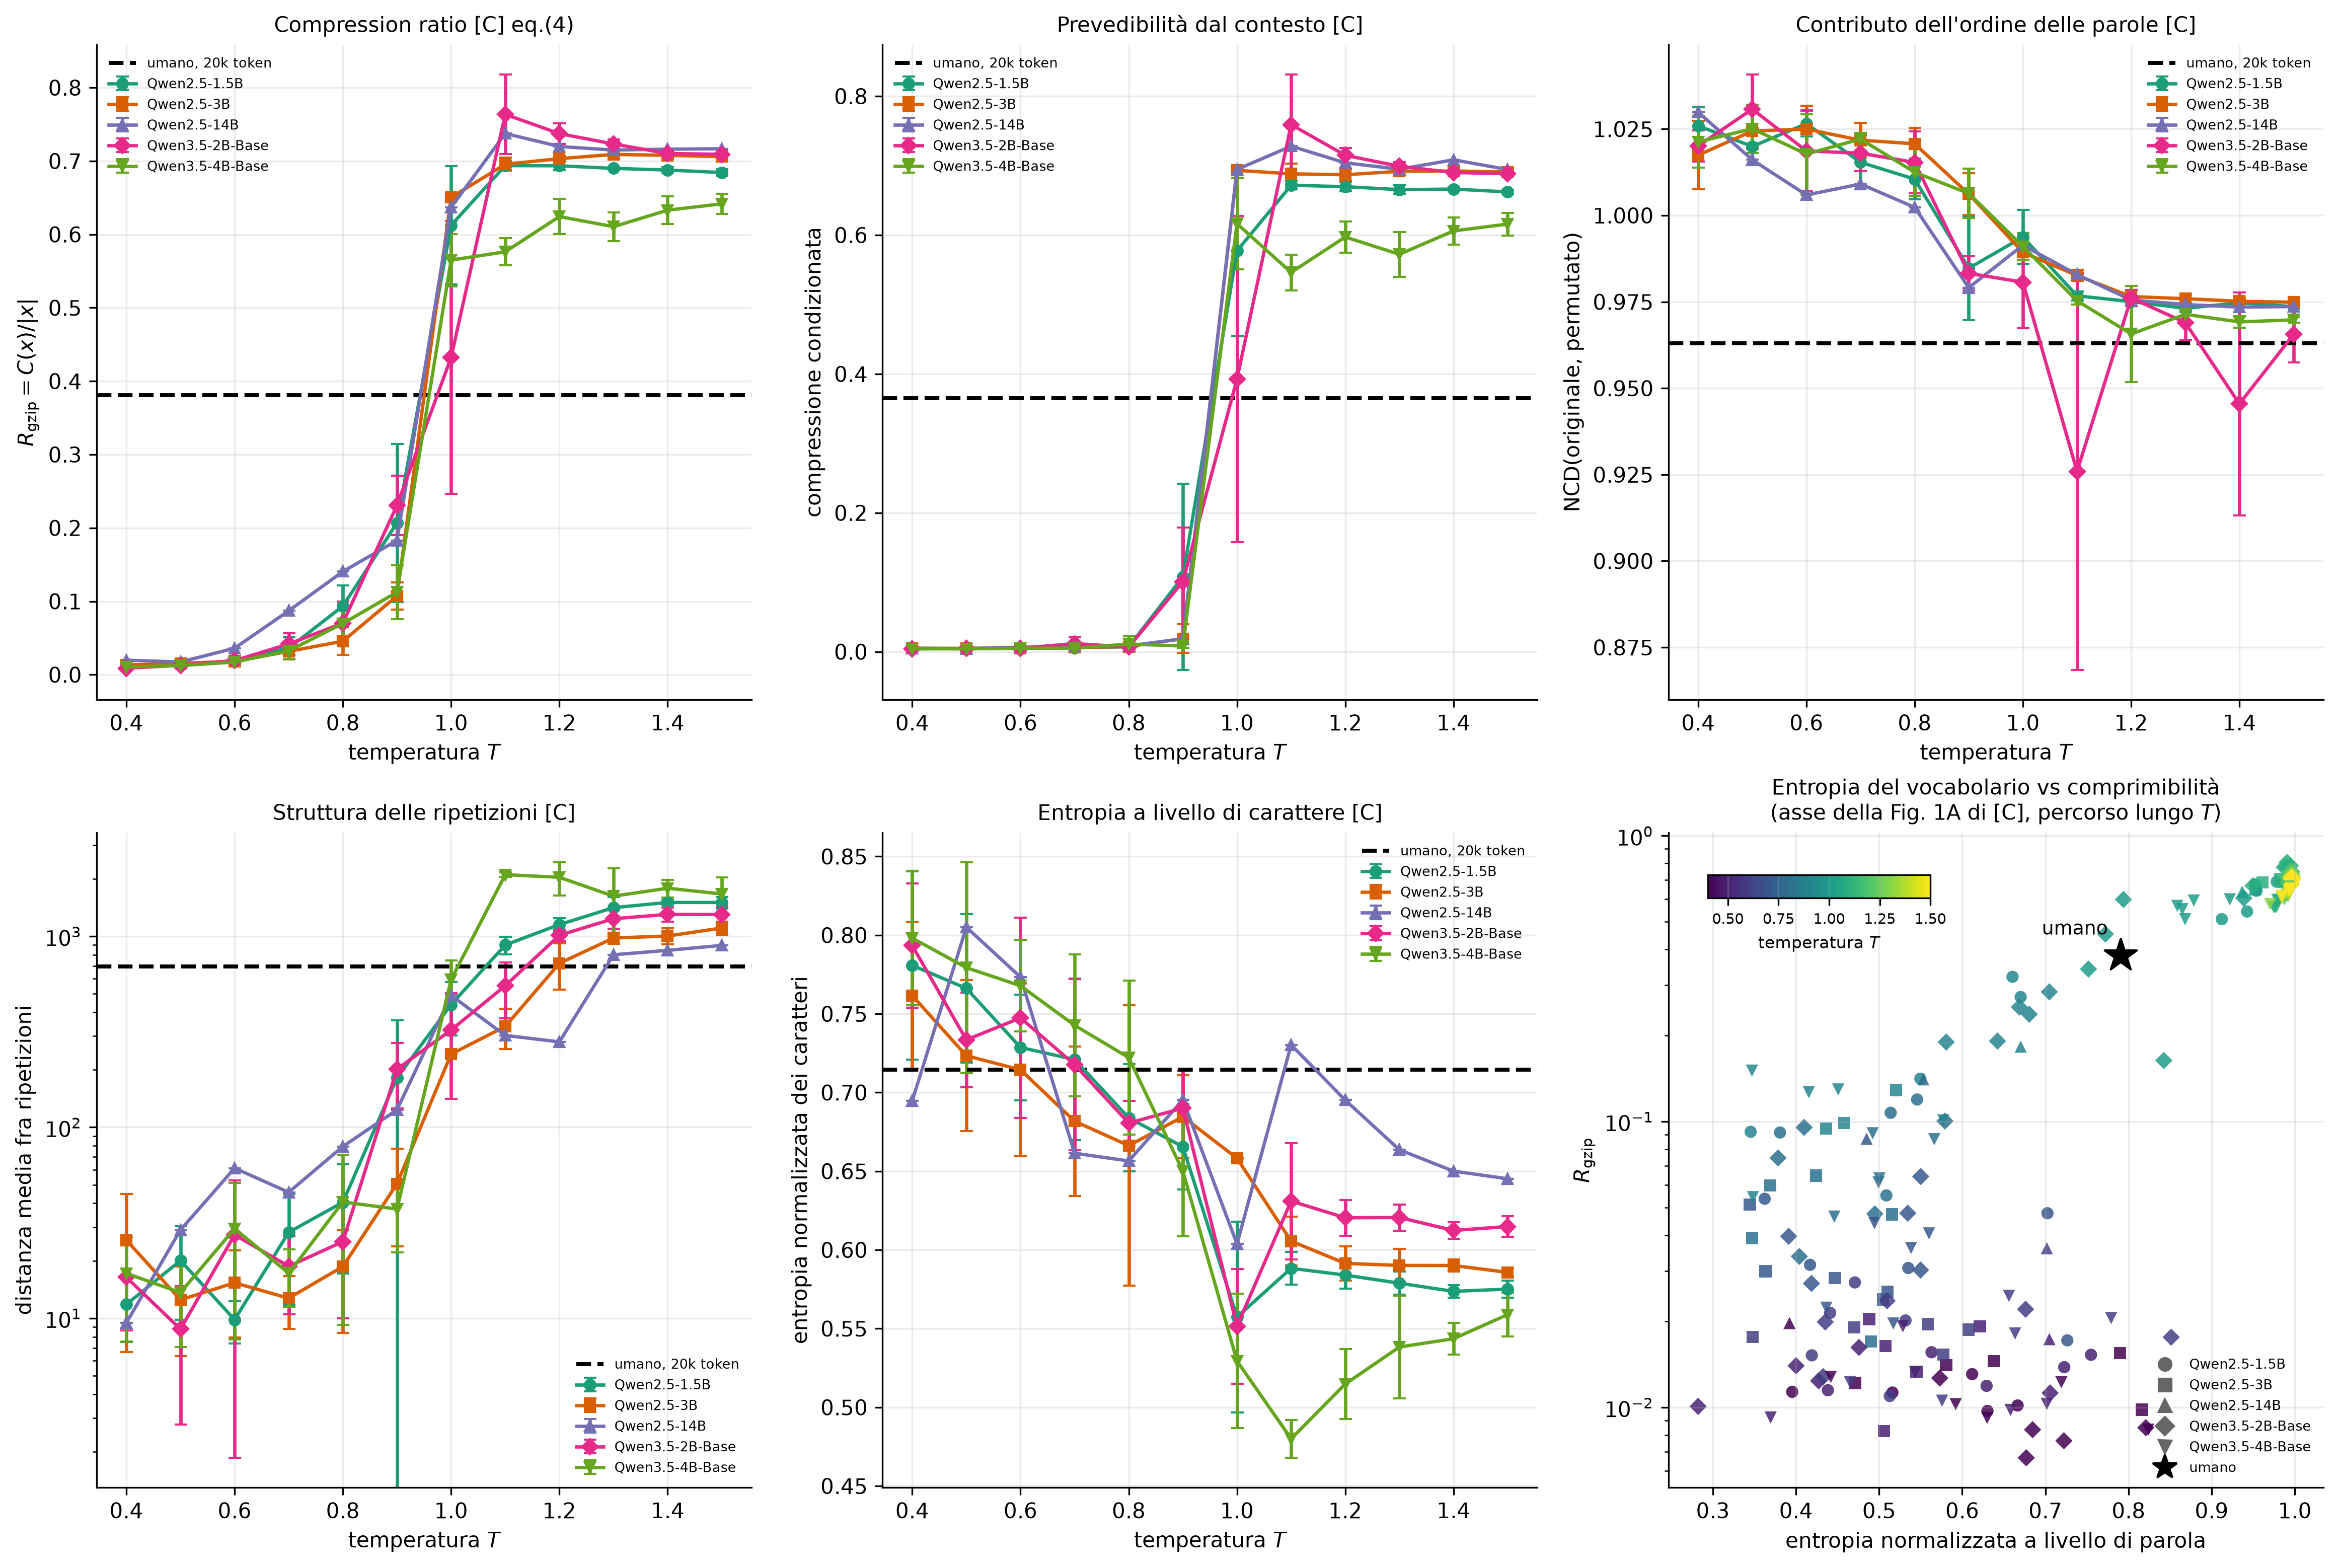
\includegraphics[width=\textwidth]{figure/cap4_compressione.png}
  \caption{Sei misure basate su compressione. Le prime cinque sono riportate in
  funzione della temperatura; l'ultima, in basso a destra, riporta il rapporto
  di compressione contro
  l'entropia normalizzata a livello di parola: è il piano della Figura~1A
  di~\cite{hadad2026}, percorso qui facendo variare la temperatura, con il testo
  umano segnato da una stella. In quel pannello il colore codifica la
  temperatura e la forma del marcatore il modello, e la scala verticale è
  logaritmica.}
  \label{fig:compressione}
\end{figure}

Il rapporto di compressione è la misura che separa i regimi in modo più netto di
tutte le altre. Per il modello esemplare passa da $0.013$ a $T = 0.4$ a $0.107$
a $T = 0.9$ e a $0.650$ a $T = 1.0$: un fattore cinquanta fra i due estremi, con
un salto di un fattore sei concentrato in un singolo passo di temperatura. Il
valore umano è $0.381$, e viene attraversato fra $T = 0.9$ e $T = 1.0$ come
tutte le altre misure del capitolo.

Il lavoro di~\cite{hadad2026} riporta che il testo generato è più regolare e
più comprimibile di quello umano, mentre qui il rapporto di compressione
supera il valore umano sopra $T = 1.0$. Le due osservazioni non sono in
contrasto, perché descrivono regioni diverse dello stesso asse: sotto la
transizione il testo generato è molto più comprimibile del testo umano,
$0.013$ contro $0.381$, ed è il regime in cui i modelli operano con le
impostazioni ordinarie; sopra la transizione la comprimibilità cade perché il
testo cessa di essere linguaggio, non perché acquisti struttura.

La compressione condizionata si comporta in modo analogo ma dice qualcosa di
diverso. Fino a $T = 0.9$ vale meno di $0.02$: la seconda metà del documento è
quasi interamente prevedibile dalla prima, come è ovvio in un testo che ripete
lo stesso ciclo. Da $T = 1.0$ sale a circa $0.69$, quasi il doppio del valore
umano $0.365$: la seconda metà è ora \emph{meno} prevedibile dalla prima di
quanto lo sia in un romanzo. Fra i due regimi non esiste una temperatura in cui
la predicibilità dal contesto assomigli a quella del testo umano.

Il salto oltre il valore umano non è una particolarità del modello esemplare. La
mediana su tutti e cinque i modelli passa da $0.015$ a $T = 0.9$ a $0.627$ a
$T = 1.0$, e il singolo modello che si avvicina di più al valore umano da sotto,
il Qwen3.5-2B-Base con $0.135$, lo scavalca comunque in un passo arrivando a
$0.430$. Nessuno dei cinque si ferma sul valore umano, ed è l'unica delle misure
di questo capitolo per cui ciò accade.

\paragraph{Il piano entropia--comprimibilità.}
Il pannello in basso a destra della Figura~\ref{fig:compressione} colloca i
documenti nel piano definito da~\cite{hadad2026}, percorso qui da un modello
reale al variare di un solo parametro anziché da distribuzioni artificiali, con
il testo umano in posizione intermedia. L'asse verticale è logaritmico perché il rapporto di compressione
non si annulla mai: il valore più basso osservato è $0.0067$. Su un asse
lineare esteso fino a $0.81$, però, i 57 documenti che stanno fra $0.007$ e
$0.020$, quasi un quarto del totale, si sovrappongono tutti sulla linea dello
zero, e la loro struttura interna scompare. In scala logaritmica si vede
invece che occupano un intervallo di entropia molto ampio, da $0.28$ a $0.85$,
e la ragione è che le due grandezze misurano cose diverse. Il rapporto di
compressione dipende dalla ripetizione della sequenza: un testo che ripete
sempre lo stesso ciclo si comprime a poco più dell'un per cento della sua
dimensione, qualunque sia il numero di parole che il ciclo contiene.
L'entropia normalizzata dipende invece dalla forma della distribuzione delle
frequenze su quel vocabolario ridotto, che conta fra 37 e 235 tipi distinti.
Un ciclo lungo e vario e un ciclo corto e povero sono ugualmente comprimibili
ma hanno entropie molto diverse: da qui la dispersione orizzontale della
nuvola a bassa comprimibilità.

\paragraph{La lunghezza del ciclo, misurata.}
L'argomento appena esposto invoca una grandezza che le misure di questo capitolo
non contengono, la lunghezza del ciclo ripetuto, ed è quindi il caso di
misurarla. Sulla successione di parole di ciascun documento si cerca il più
piccolo sfasamento $L_{\mathrm{ciclo}}$ per cui l'accordo fra la parola in
posizione $i$ e quella in posizione $i - L_{\mathrm{ciclo}}$, calcolato sugli
ultimi venti giri, supera il novanta per cento. La finestra di verifica è locale
e commisurata al periodo candidato: su tutto il testo la prosa che precede il
ciclo diluirebbe la media, mentre su un suffisso lungo un ciclo che cambia
lentamente variante scende sotto soglia al proprio periodo e la supera a un
multiplo, restituendo un alias. La soglia è fissata al novanta e non al cento
per cento per tollerare i cicli non esattamente verbatim; l'accordo atteso per
caso in prosa inglese è circa $0.05$, quindi non vi sono falsi positivi.

Il criterio individua \num{113} documenti su \num{242}, e sono tutti a
$T \le 0.9$: la totalità fino a $T = 0.7$, il $95\%$ a $T = 0.8$, il $56\%$ a
$T = 0.9$ e nessuno da
$T = 1.0$ in poi. Coincidono con la nuvola a bassa comprimibilità: tutti e
cinquantasette i documenti con $R_{\mathrm{gzip}} < 0.02$ sono fra questi. Il
ciclo va da una sola parola a \num{248}, in caratteri da $9$ a \num{1127}, con
mediana di $16$ parole.

La Figura~\ref{fig:ciclo} riporta la relazione con le due grandezze del piano.
Con l'entropia di parola la correlazione di rango vale $\rho = +0.65$, e non è
un effetto della temperatura: calcolata fra documenti generati alla stessa
temperatura sale a $+0.69$, ed è positiva in tutti e sei i gruppi. Con il
rapporto di compressione, invece, non c'è relazione: $\rho = -0.15$ con
$p = 0.12$, e a temperatura fissata il segno si inverte, $+0.16$ con
$p = 0.11$. A parità di lunghezza del ciclo il rapporto di compressione varia di
un fattore compreso fra quattordici e ventisette.

Il meccanismo è quello anticipato sopra, e la misura lo rende esplicito: la
lunghezza del ciclo coincide quasi con il numero di tipi distinti che esso
contiene, $\rho = +0.84$, cosicché un ciclo corto concentra tutta la massa di
probabilità su poche parole e uno lungo la distribuisce. Gli estremi lo
mostrano nel modo più diretto: il ciclo più corto osservato è una sola parola,
ripetuta, con entropia $0.35$; il più lungo conta \num{248} parole e undici
tipi distinti, \emph{You are a bad father. You are a bad lover of children.
You are not to blame} con variazioni, con entropia $0.47$ e $R_{\mathrm{gzip}}
= 0.019$, cioè testo ancora ultracomprimibile. La lunghezza del ciclo spiega
dunque l'ordinamento lungo l'asse orizzontale del piano, non tutta la sua
dispersione: la regressione su $\log L_{\mathrm{ciclo}}$ rende conto del
$42\%$ della varianza dell'entropia.

\begin{figure}[htbp]
  \centering
  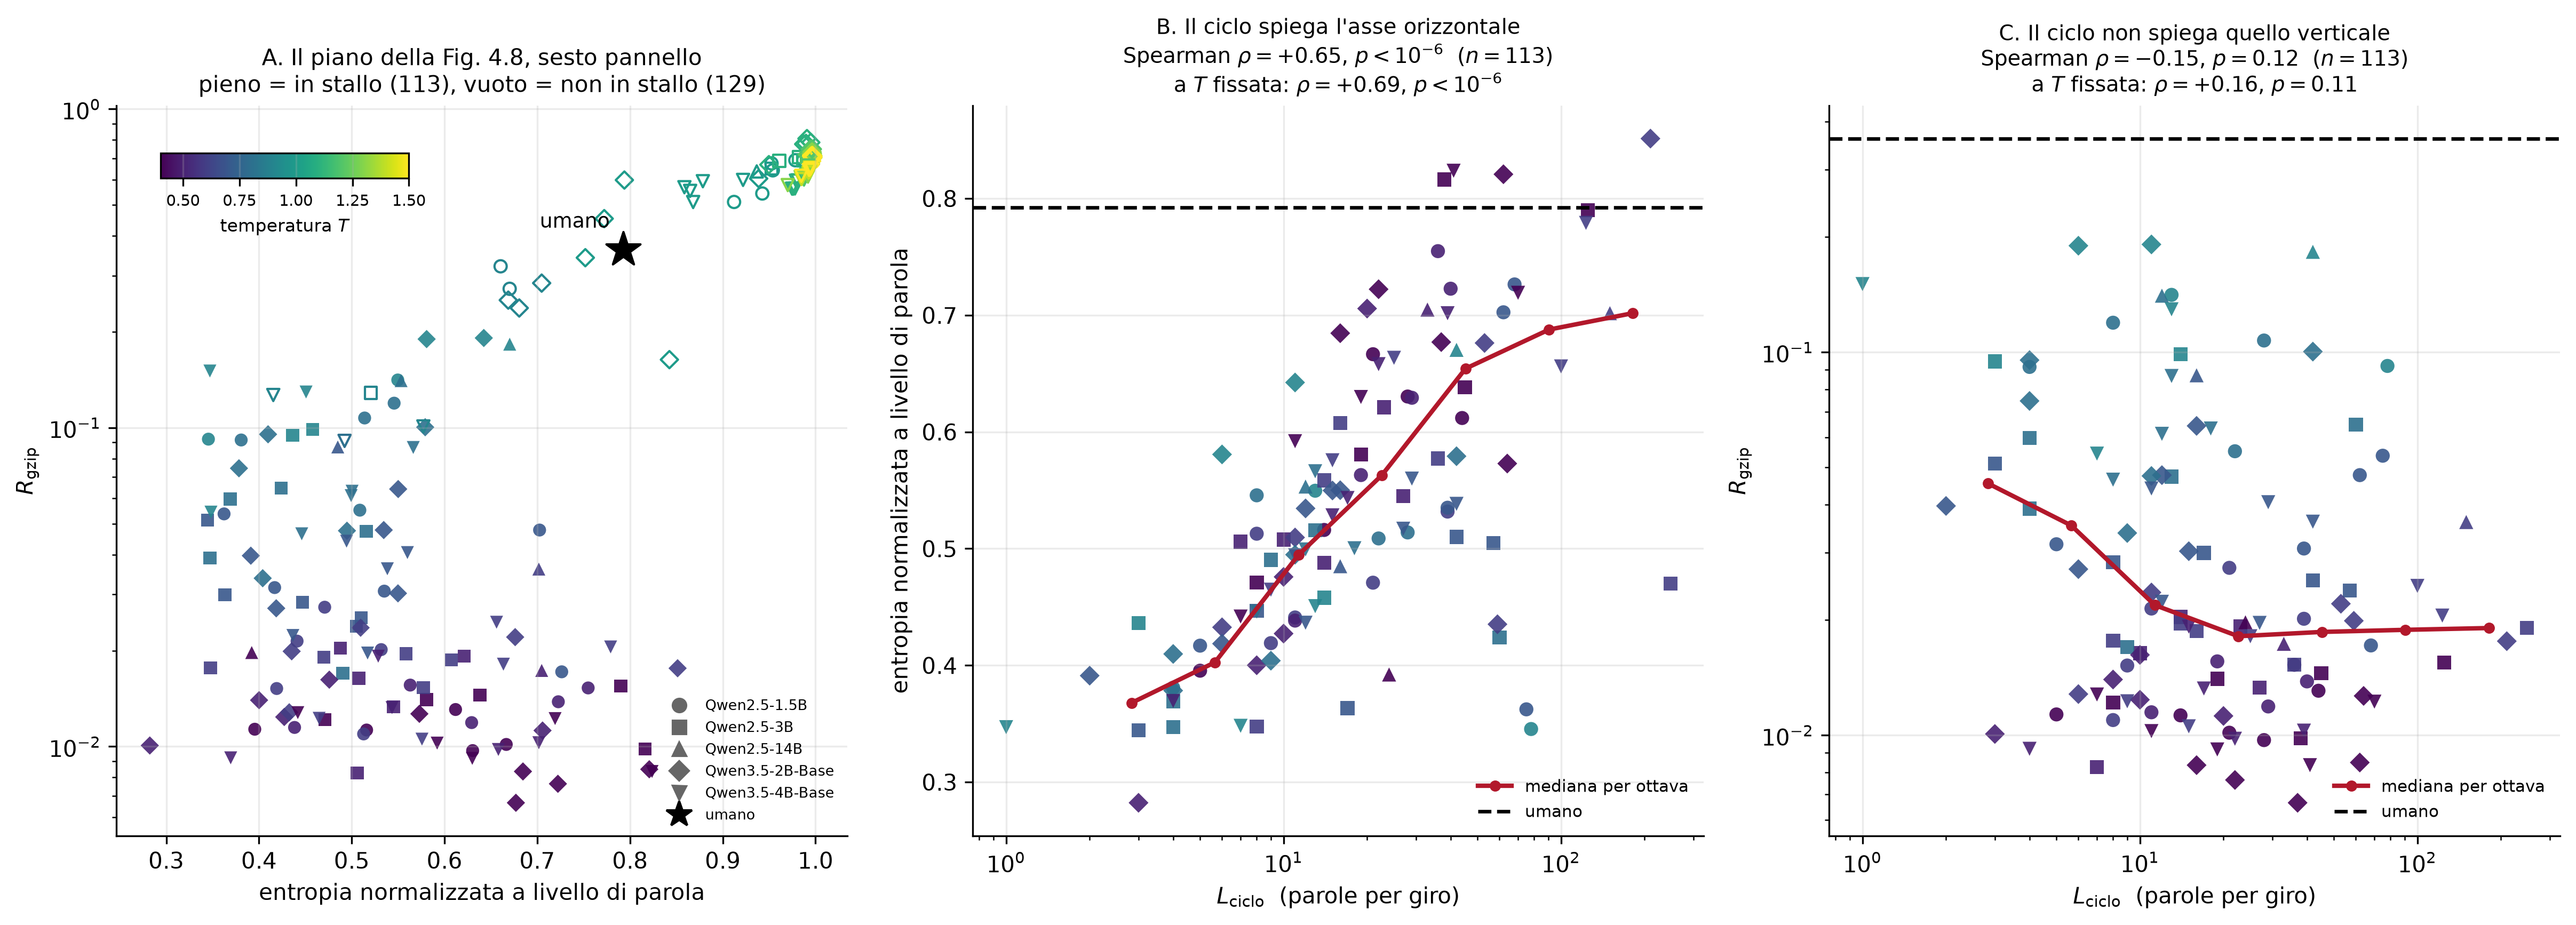
\includegraphics[width=\textwidth]{figure/cap4_ciclo_entropia.png}
  \caption{Lunghezza del ciclo ripetuto in fase di stallo. A: il piano
  entropia--comprimibilità della Figura~\ref{fig:compressione}, con i documenti
  in stallo a simbolo pieno e gli altri a simbolo vuoto; il colore codifica la
  temperatura e la forma il modello. B: entropia di parola contro lunghezza del
  ciclo, con la mediana per ottava. C: rapporto di compressione contro la stessa
  grandezza. La lunghezza del ciclo ordina l'asse orizzontale del piano e non
  quello verticale.}
  \label{fig:ciclo}
\end{figure}


% ---------------------------------------------------------------------
\section{Le tre fasi}
\label{sec:fasi-risultati}

Le misure precedenti descrivono il testo generato senza classificarlo. La regola
del §\ref{sec:tre-fasi} permette invece di assegnare ciascun documento a una
fase, e questa sezione ne riporta l'esito.

La traiettoria della~\eqref{eq:traiettoria} è costruita sui vettori GloVe a 100
dimensioni già impiegati nel §\ref{sec:token}, e l'autocorrelazione è calcolata
sui primi cento lag, misurati in parole. Il fit del GAPELMAPER usa invece un
intervallo più ampio, fino a 600 parole, perché distinguere una legge di potenza
da un esponenziale richiede più di una decade di distanze. Il livello di rumore
$\eta$ è stimato su una singola permutazione della traiettoria di ciascun
documento, con seme fissato.

Le due soglie della regola valgono $\kappa_{\min} = 0.50$ e $\Phi_{\min} = 3$.
La prima è deliberatamente permissiva: serve a escludere i documenti in cui meno
di metà delle parole ha un vettore, cioè quelli in cui la traiettoria è fatta per
lo più di zeri, e non a selezionare i documenti buoni. La seconda separa i due
gruppi in cui $\Phi$ effettivamente si distribuisce, e la sua posizione è poco
critica: come mostra la Figura~\ref{fig:transizioni}, fra la fase periodica e
quella successiva $\Phi$ cambia di due ordini di grandezza, cosicché qualunque
soglia compresa fra $1$ e $5$ produce la stessa classificazione. Il
§\ref{sec:tstar} riprende il punto trattando la fine della fase periodica come
uno degli otto criteri di temperatura critica.

La Figura~\ref{fig:acf} mostra come questa autocorrelazione cambia lungo lo
sweep. Fino a $T = 0.9$ la curva oscilla con periodo definito e ampiezza
prossima all'unità: il testo ripete un ciclo di parole, e a distanza pari a un
multiplo del ciclo ogni vettore ritrova sé stesso. Il periodo si accorcia al
crescere della temperatura, da dieci parole a $T = 0.5$ a circa tre a $T =
0.8$, mentre l'ampiezza scende da $0.98$ a $0.72$. Fra $T = 0.9$ e $T = 1.0$
la struttura periodica scompare del tutto: l'ampiezza cade a $0.036$ e la
curva diventa un decadimento monotono, senza più oscillazione. A $T = 1.3$
l'intera curva è contenuta nella banda di rumore stimata mescolando le parole
del documento, cioè non è distinguibile dal caso.

Il confronto con il testo umano chiarisce quanto entrambi i regimi siano
lontani dal linguaggio naturale. L'autocorrelazione del romanzo non è
periodica, con $\max\lvert\mathrm{FFT}\rvert$ pari a $1.16$, ben sotto la
soglia $3$, ma è nettamente sopra il livello di rumore su tutti i cento lag
esaminati, e il suo spettro decade in modo regolare invece di essere piatto.
Nessuna delle temperature campionate riproduce questa combinazione: sotto la
transizione la correlazione è troppo forte e periodica, sopra è assente.

\begin{figure}[htbp]
  \centering
  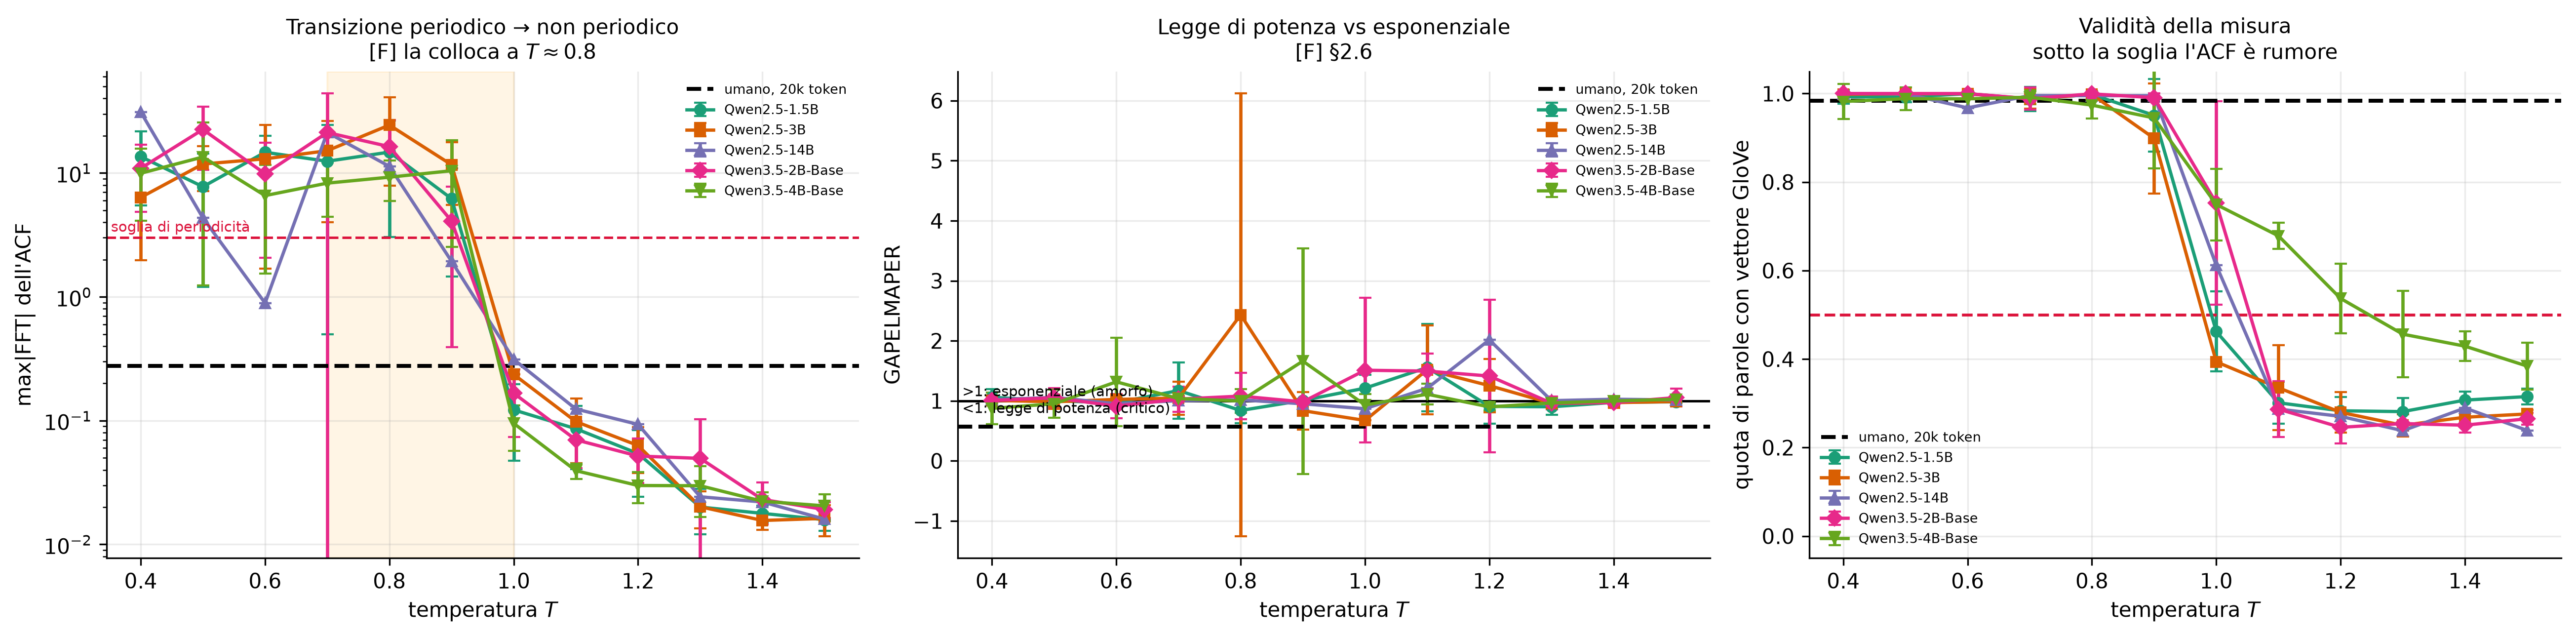
\includegraphics[width=\textwidth]{figure/cap4_transizioni_fase.png}
  \caption{Parametro di periodicità, GAPELMAPER e copertura degli embedding in
  funzione della temperatura. Il primo pannello è in scala logaritmica. Il terzo
  riporta la quota di parole dotate di un vettore, che è la condizione di
  validità delle altre due misure.}
  \label{fig:transizioni}
\end{figure}

\begin{figure}[htbp]
  \centering
  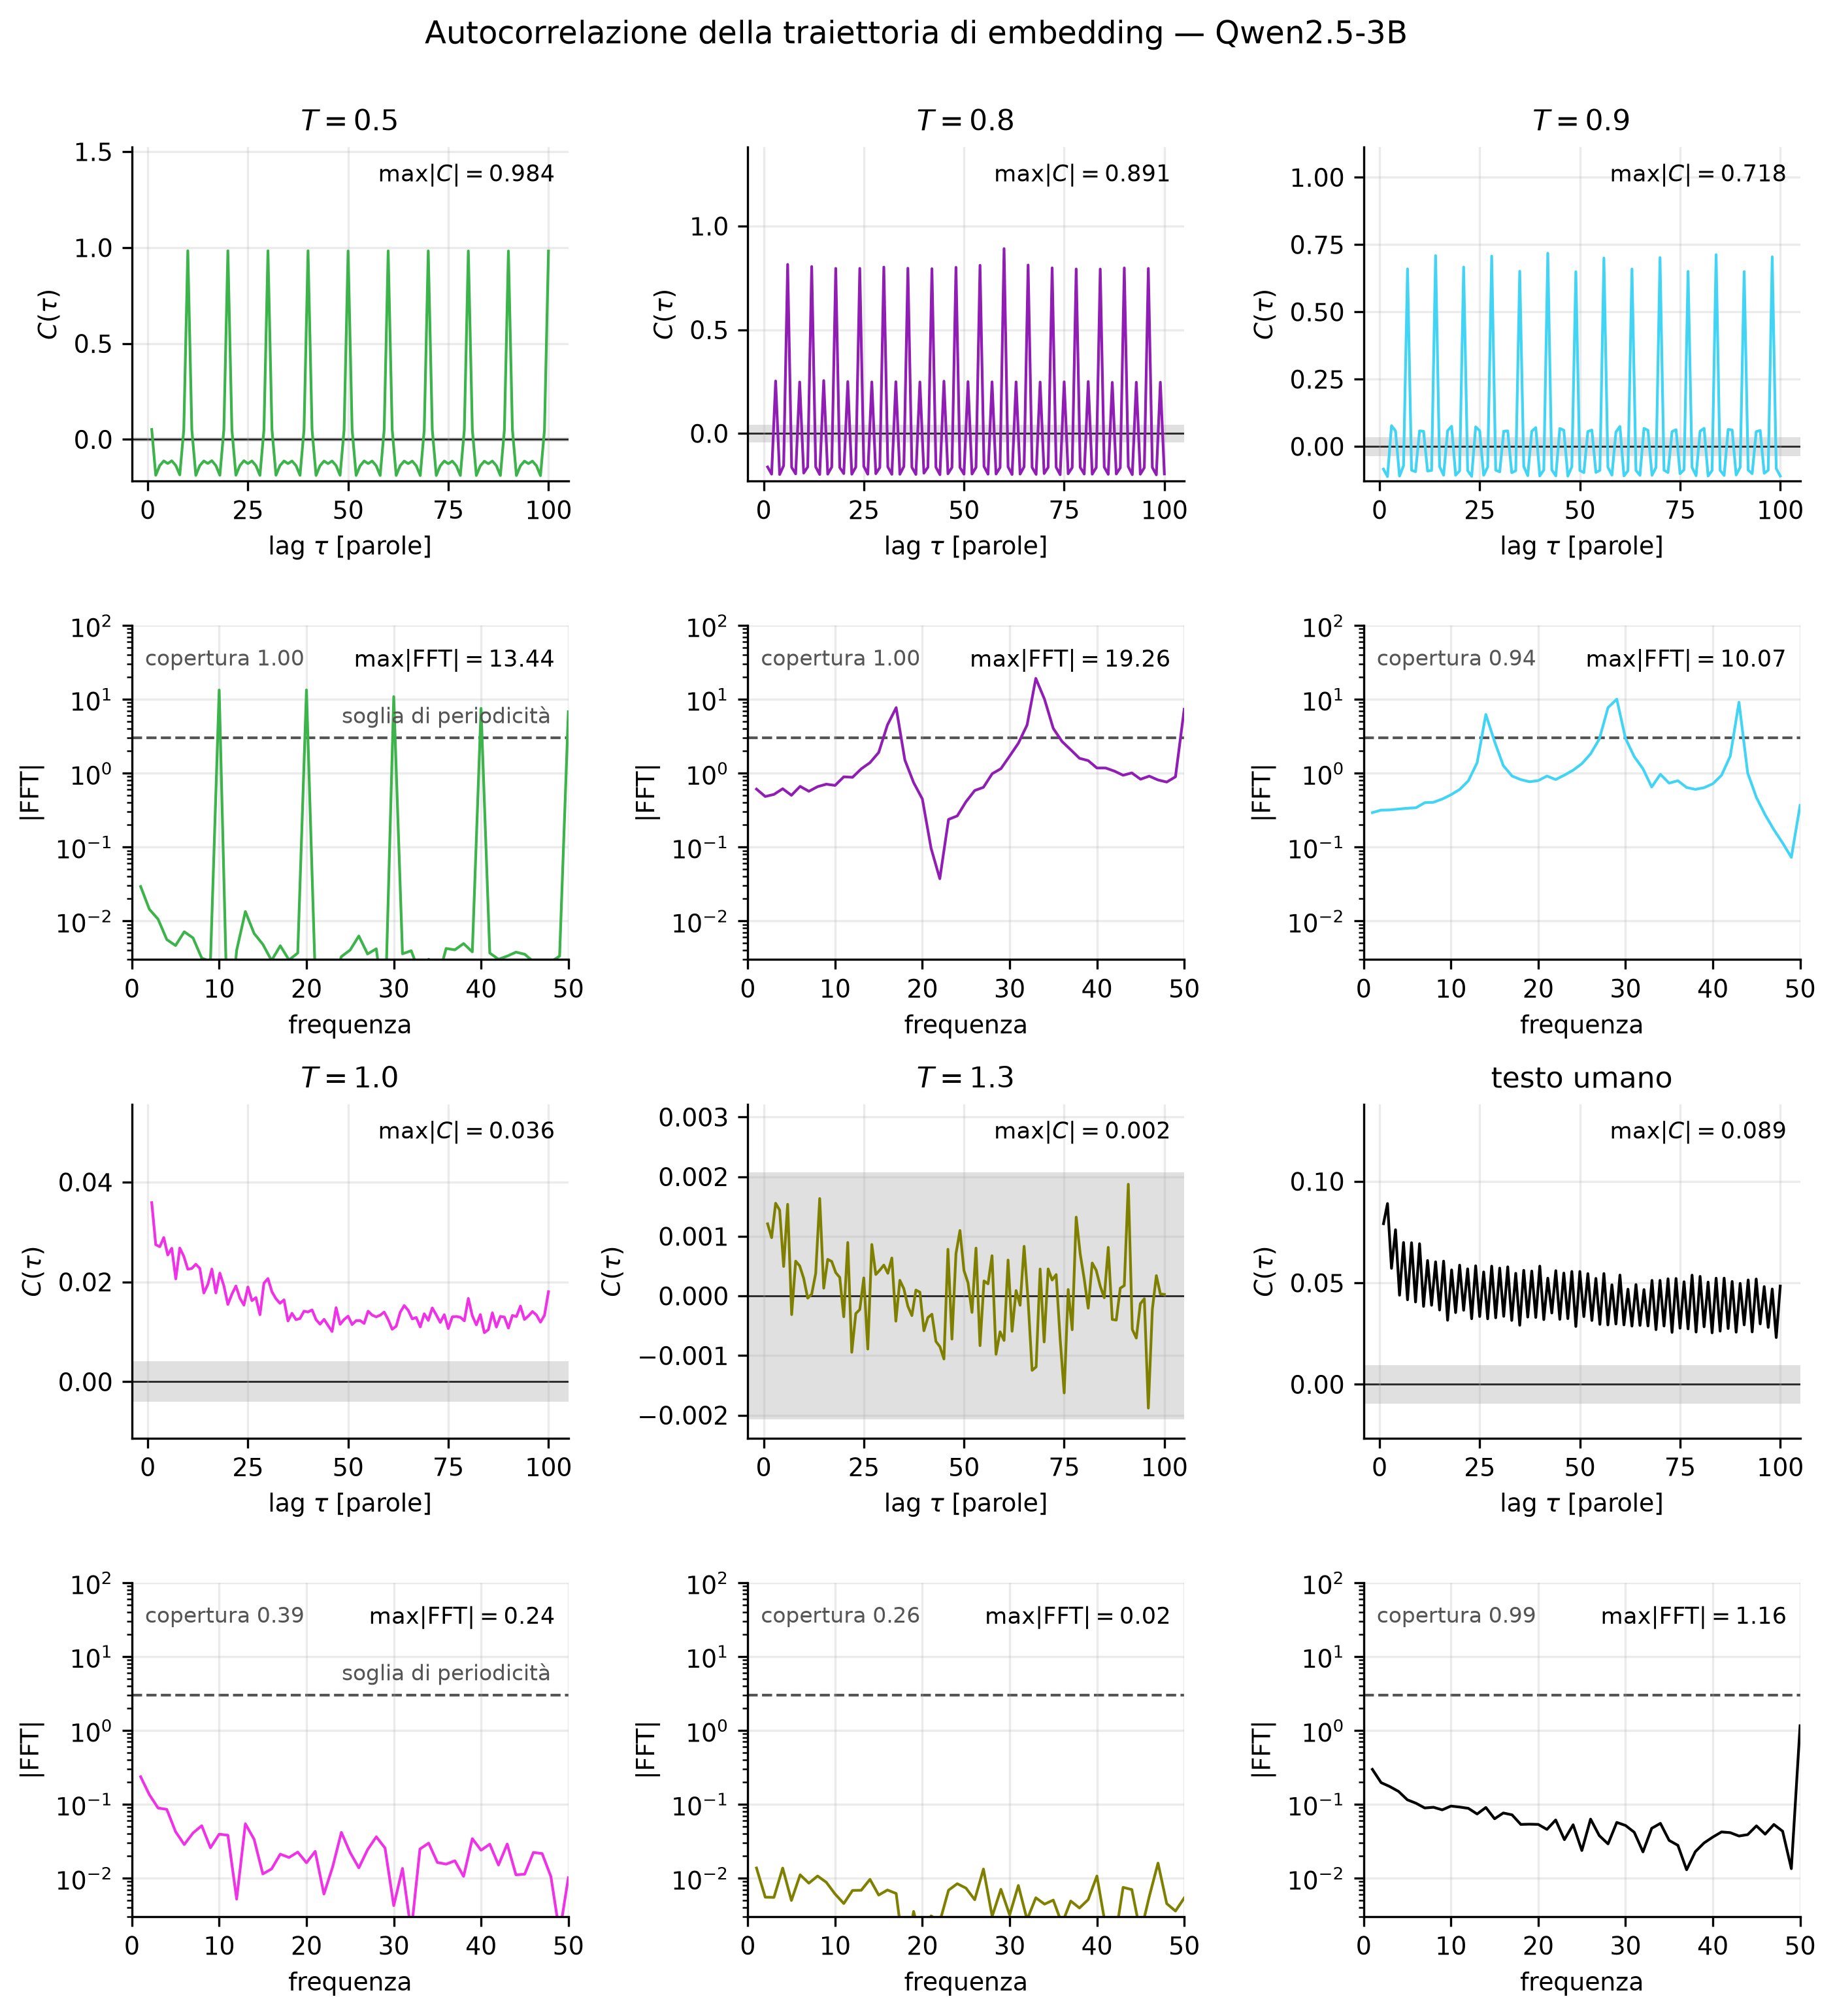
\includegraphics[width=\textwidth]{figure/cap4_acf_Qwen25_3B.png}
  \caption{Autocorrelazione della traiettoria di embedding per il modello
  Qwen2.5-3B a cinque temperature e sul testo umano di riferimento. In ciascuna
  coppia di riquadri il primo riporta $C(\tau)$ per lag da 1 a 100 parole e il
  secondo il modulo della sua trasformata di Fourier. La banda grigia è il
  livello di rumore, stimato ricalcolando $C(\tau)$ dopo aver permutato a caso
  le parole dello stesso documento; la linea tratteggiata è la soglia
  $\max\lvert\mathrm{FFT}\rvert = 3$ che separa la fase periodica. Per ogni
  temperatura è mostrato il campione di periodicità mediana, non il più marcato.
  La scala verticale di $C(\tau)$ è propria di ciascun riquadro, perché
  l'ampiezza varia di oltre due ordini di grandezza fra le temperature basse e
  quelle alte; il valore di picco è riportato dentro il riquadro. La scala dello
  spettro è invece logaritmica e comune, così i sei casi si confrontano
  direttamente.}
  \label{fig:acf}
\end{figure}

Il parametro d'ordine della prima transizione è il massimo modulo della
trasformata oltre il primo coefficiente, e il suo crollo è il risultato più
netto dell'intero capitolo. La media su tutti i modelli vale $16.0$ a
$T = 0.8$, scende a $7.5$ a $T = 0.9$ e precipita a $0.145$ a $T = 1.0$: un
fattore cinquanta in un solo passo di temperatura, e cento rispetto al massimo
di $T = 0.8$. Prosegue poi fino a $0.018$ a
$T = 1.5$, complessivamente tre ordini di grandezza sotto il massimo. Le cinque
curve dei diversi modelli si sovrappongono quasi esattamente, come mostra la
Figura~\ref{fig:transizioni}.

Anche questa soglia va confrontata con la fonte.
In~\cite{mikhaylovskiy2025states} la transizione dalla fase periodica è
collocata attorno a $t = 0.8$, con il testo dichiarato già non periodico a
$t = 1$, mentre qui la periodicità sopravvive fino a $T = 0.9$ e scompare a
$T = 1.0$. Lo spostamento verso l'alto è coerente con l'effetto del prompt
descritto nel §\ref{sec:protocollo}, che ritarda la comparsa delle proprietà
del regime disordinato.

\paragraph{Il secondo criterio non discrimina.} La distinzione fra stato
critico e fase amorfa dovrebbe essere operata dal GAPELMAPER, ma sui dati di
questo lavoro tale criterio non funziona. Il suo valore medio è $1.101$ con
deviazione standard $0.677$, e la quota di documenti con valore inferiore a 1,
cioè classificati come critici, è $0.51$: una moneta. Le barre d'errore nel
pannello centrale della Figura~\ref{fig:transizioni} sono di ampiezza
confrontabile con l'intero intervallo di variazione.

La difficoltà non è propria di questi dati. Lo stesso
\cite{mikhaylovskiy2025states} riporta che sui testi Qwen il GAPELMAPER è
raramente inferiore a 1, e che a diverse temperature del suo sweep non è
calcolabile affatto perché l'autocorrelazione assume valori negativi. Il
criterio, insomma, discrimina male anche nel lavoro che lo introduce.

Il motivo emerge dal terzo pannello. La copertura degli embedding resta sopra il
$95\%$ fino a $T = 0.9$, ma crolla a $0.64$ a $T = 1.0$ e a circa $0.31$ oltre
$T = 1.2$: nel regime in cui il GAPELMAPER dovrebbe distinguere le ultime due
fasi, l'autocorrelazione è calcolata su una minoranza delle parole e non
contiene più segnale. Per questa ragione i documenti che non superano la soglia
di copertura sono marcati come non valutabili anziché classificati, come
anticipato nel §\ref{sec:tre-fasi}. Senza tale precauzione il criterio avrebbe
assegnato una fase a documenti in cui non c'è nulla da misurare.

\paragraph{Il diagramma di fase.}
La Figura~\ref{fig:diagramma} riporta la composizione delle fasi per modello e
temperatura. Il quadro è coerente su tutti e cinque: fase periodica fino a
$T = 0.9$, dove la classificazione è ancora periodica per 13 documenti su 18;
scomparsa completa della periodicità a $T = 1.0$; documenti prevalentemente non
valutabili da $T = 1.1$ in poi, e completamente tali a $T \ge 1.4$.

\begin{figure}[htbp]
  \centering
  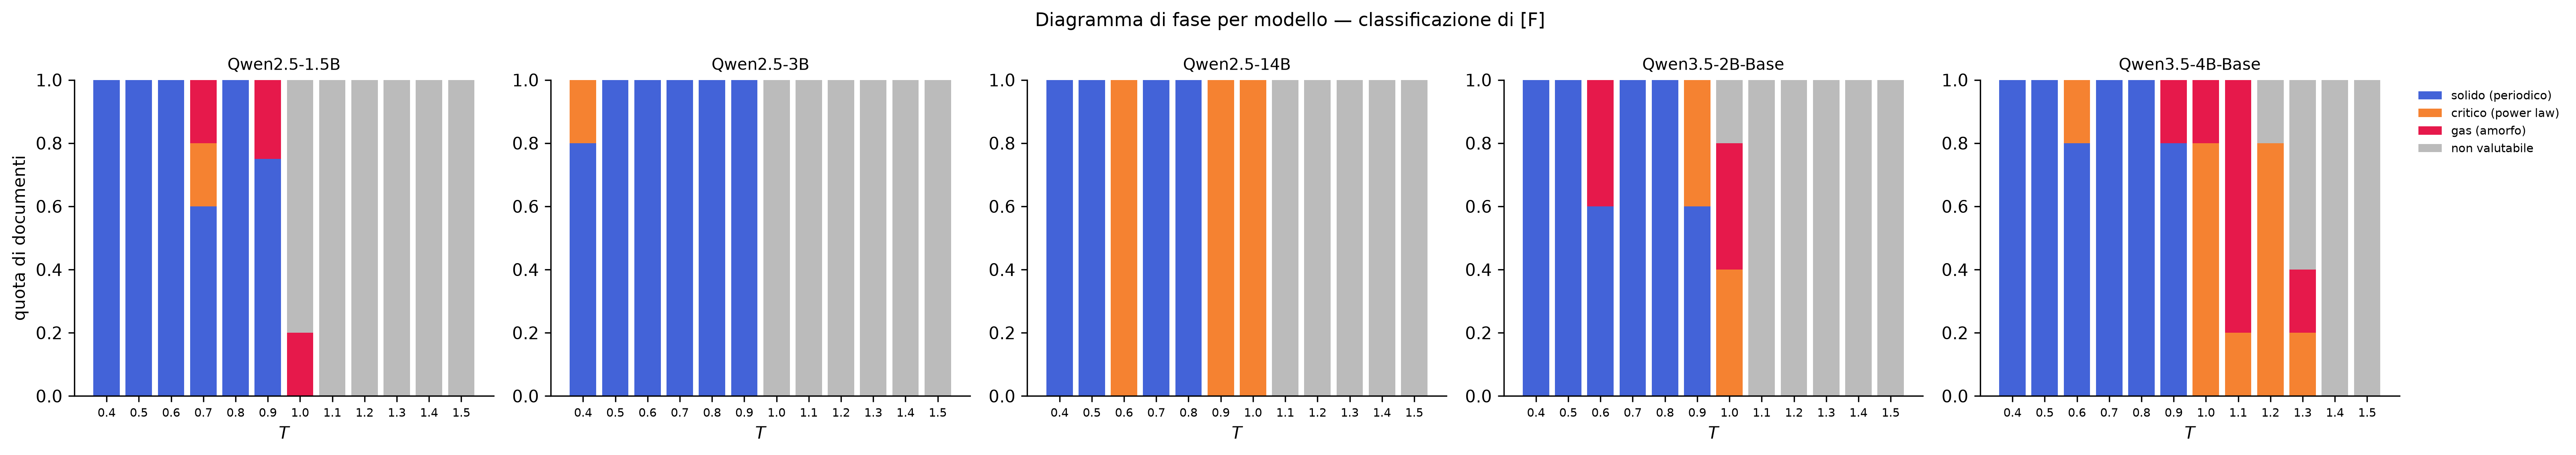
\includegraphics[width=\textwidth]{figure/cap4_diagramma_fase.png}
  \caption{Composizione delle fasi per modello e temperatura. La categoria «non
  valutabile» raccoglie i documenti che non superano la soglia di copertura
  degli embedding.}
  \label{fig:diagramma}
\end{figure}

Le tre modalità di fallimento del §\ref{sec:fallimenti} trovano qui la loro
interpretazione. La degenerazione per ripetizione è la fase periodica; la
degenerazione dell'alfabeto e del lessico corrisponde alla regione in cui la
misura non è più applicabile, che è a sua volta il segnale della fase amorfa. Il
testo non degenerato esiste solo nella striscia sottile fra le due, ed è la
stessa striscia in cui tutte le misure delle sezioni precedenti si avvicinano ai
valori umani.

% ---------------------------------------------------------------------
\section{Convergenza della temperatura critica}
\label{sec:tstar}

Le sezioni precedenti individuano ciascuna una temperatura privilegiata. Poiché
i criteri provengono da lavori indipendenti e misurano proprietà diverse del
testo, il loro accordo o disaccordo è esso stesso un risultato.

La Tabella~\ref{tab:tstar} riporta la temperatura selezionata da ciascun
criterio per ciascun modello. Due criteri sono intrinseci, nel senso che
individuano un estremo della curva senza far riferimento al testo umano: il
minimo del MAPE e la fine della fase periodica. Gli altri sei selezionano la
temperatura alla quale la misura si avvicina di più alla baseline umana.

\begin{table}[htbp]
\centering
\small
\begin{tabular}{@{}lccccc@{}}
\toprule
Criterio & 1.5B & 3B & 14B & 3.5-2B & 3.5-4B \\
\midrule
MAPE minimo                                  & 0.9 & 0.9 & 0.7 & 0.9 & 0.9 \\
$D_s$ minima dal testo umano                 & 0.9 & 0.9 & 0.9 & 0.9 & 1.0 \\
Fine della fase periodica                    & 1.0 & 1.0 & 0.6 & 1.0 & 1.0 \\
$R_{\mathrm{gzip}}$ più vicino all'umano     & 0.9 & 1.0 & 0.9 & 1.0 & 1.0 \\
$\alpha$ più vicino all'umano                & 1.0 & 1.5 & 1.3 & 1.0 & 1.0 \\
$R$ più vicino all'umano                     & 1.0 & 1.1 & 1.1 & 1.1 & 1.0 \\
$\gamma_H$ più vicino all'umano              & 1.1 & 1.0 & 1.3 & 1.1 & 1.3 \\
$\alpha_{\mathrm{DFA}}$ più vicino all'umano & 1.2 & 1.1 & 1.1 & 1.1 & 1.1 \\
\midrule
\textbf{mediana}                             & \textbf{1.0} & \textbf{1.0} &
\textbf{1.0} & \textbf{1.0} & \textbf{1.0} \\
\bottomrule
\end{tabular}
\caption{Temperatura selezionata da ciascun criterio, per ciascun modello. La
mediana vale $1.0$ per tutti e cinque i modelli, benché i singoli criteri
spazino da $0.6$ a $1.5$.}
\label{tab:tstar}
\end{table}

Il risultato principale del capitolo è la riga in fondo alla tabella. Otto
criteri tratti da quattro lavori indipendenti, costruiti per scopi diversi e mai
progettati per concordare, danno una mediana identica per tutti e cinque i
modelli. La convergenza non era scontata: i criteri misurano la distribuzione
delle frequenze, la crescita del vocabolario, le correlazioni a lungo raggio, la
comprimibilità e la periodicità dell'autocorrelazione, cioè proprietà che nulla
obbliga a coincidere.

\begin{figure}[htbp]
  \centering
  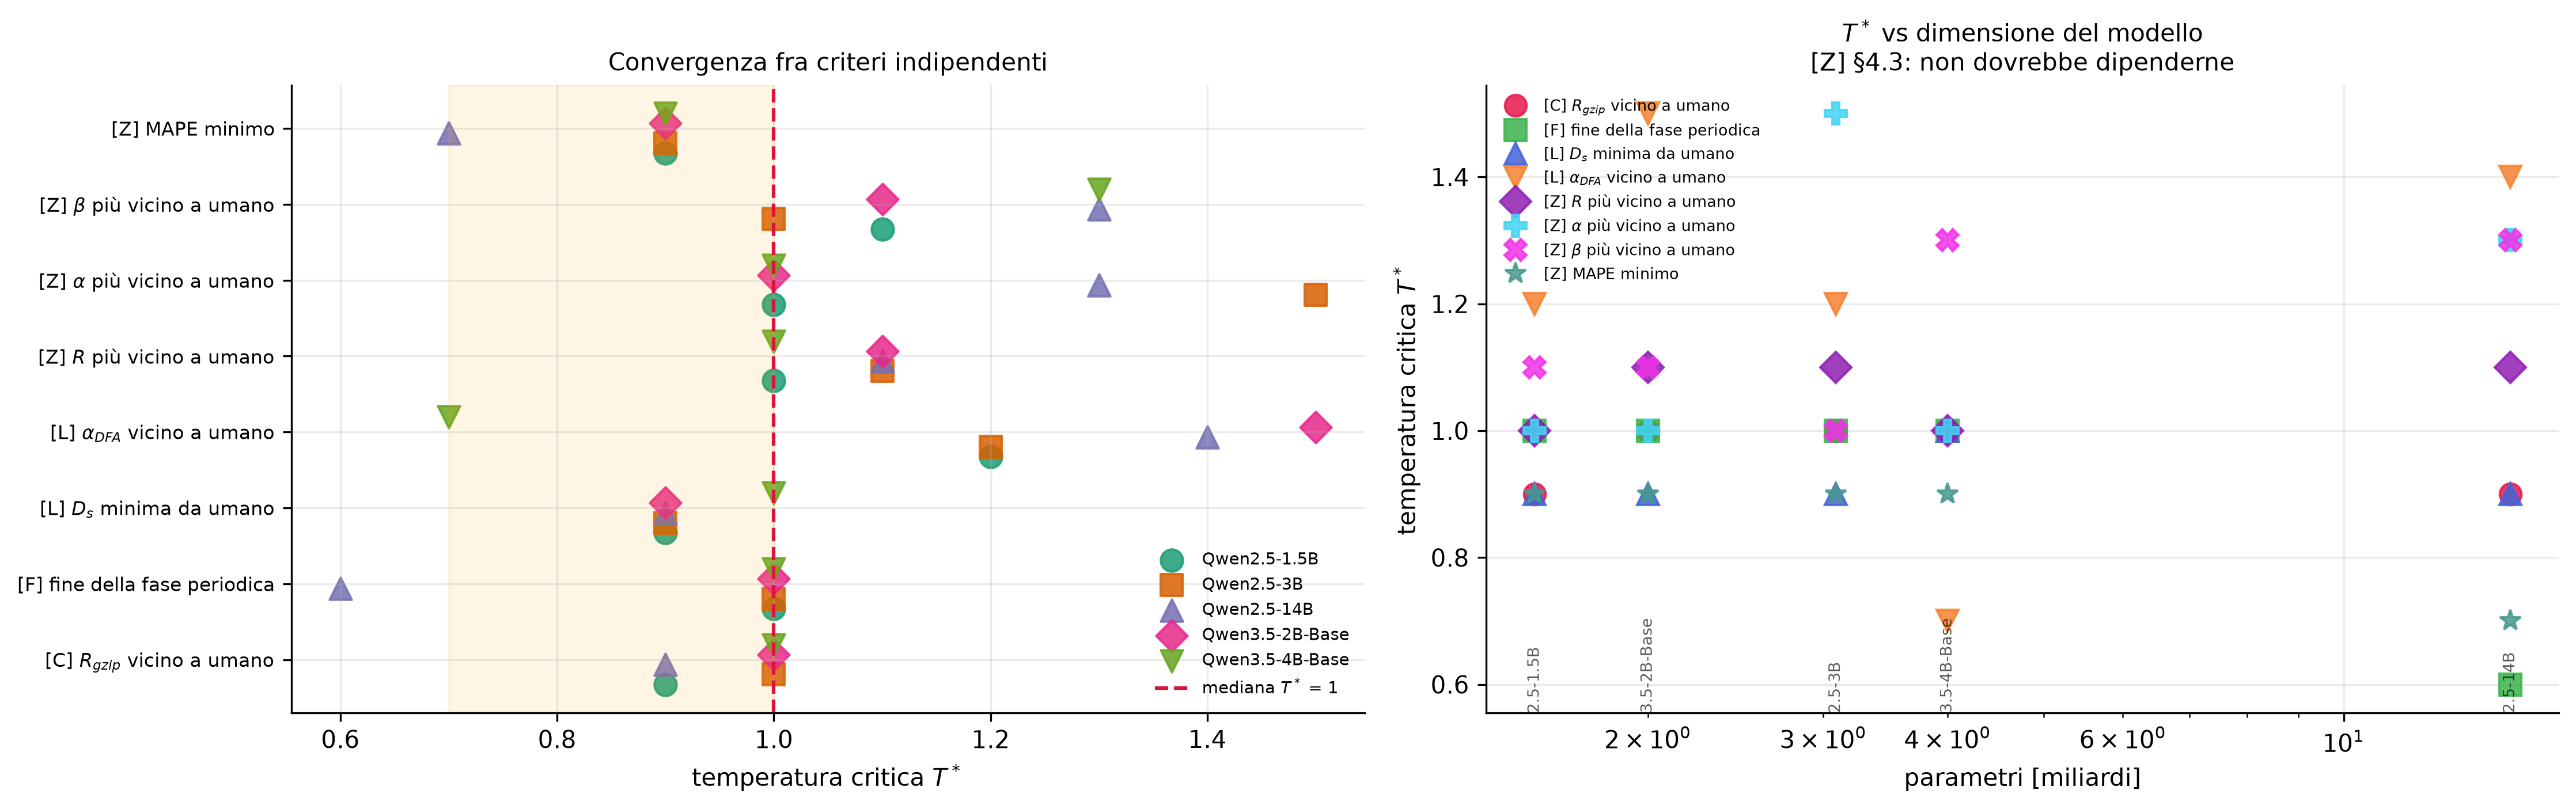
\includegraphics[width=\textwidth]{figure/cap4_temperatura_critica.png}
  \caption{A sinistra, la temperatura selezionata da ciascun criterio; la linea
  tratteggiata è la mediana complessiva e la banda la regione fra $0.7$ e $1.0$.
  A destra, la stessa quantità in funzione del numero di parametri del modello.}
  \label{fig:tstar}
\end{figure}

\paragraph{Dipendenza dalla dimensione del modello.}
La Figura~\ref{fig:tstar} riporta a destra la temperatura critica in funzione
del numero di parametri. La correlazione di rango è $\rho = -0.01$ con
$p = 0.93$ su quaranta osservazioni: nessuna dipendenza rilevabile. Il dato è
coerente con quanto riportato in~\cite{mikhaylovskiy2025zipf}, dove la posizione
dell'ottimo risulta indipendente dalla dimensione per tutte le famiglie
esaminate.

Un'assenza di correlazione misurata su cinque modelli appartenenti a due
famiglie non dimostra l'indipendenza: dimostra che, entro l'intervallo di
dimensioni esplorato e con la potenza statistica disponibile, non emerge
alcuna dipendenza. È coerenza con la letteratura, non conferma indipendente.

\paragraph{Una discordanza fra criteri.}
Due criteri si collocano sistematicamente fuori dal gruppo, e la loro distanza
dagli altri è essa stessa un risultato: mediarli insieme al resto la
cancellerebbe.

Il minimo del MAPE cade a $0.9$, mentre la fine della fase periodica cade a
$1.0$: alla temperatura in cui la distribuzione delle frequenze è più vicina a
una legge di potenza, l'autocorrelazione è ancora periodica per la maggioranza
dei documenti. Le due misure non si contraddicono, perché guardano oggetti
diversi, la statistica dei conteggi l'una e la struttura sequenziale l'altra,
e la loro distanza quantifica il fatto che le due proprietà non compaiono
simultaneamente. Il testo acquista una distribuzione di frequenze verosimile
prima di perdere la ripetizione.

Il criterio basato su $\alpha_{\mathrm{DFA}}$ merita una nota, perché il suo
esito dipende dall'ordine del detrending. Con il grado 1 seleziona temperature
fra $0.7$ e $1.5$, il più disperso dei nove; con il grado 2, che è quello
adottato qui per la ragione data nel §\ref{sec:robustezza}, si allinea agli
altri e sceglie $1.1$ per quattro modelli su cinque. La mediana per modello vale
$1.0$ in entrambi i casi. Resta valida l'avvertenza del
§\ref{sec:dfa-risultati}: alle basse temperature quell'esponente è instabile
fra documenti, e viene riportato per completezza anziché usato come criterio a
sé stante.

Una divergenza analoga fra criteri è documentata
in~\cite{mikhaylovskiy2025zipf} per i modelli Llama di grandi dimensioni, dove
le leggi di Zipf e di Heaps individuano temperature critiche sensibilmente
diverse. Il fenomeno non sembra dunque un artefatto di questo lavoro.

% ---------------------------------------------------------------------
\section{Che cosa lo sweep ha stabilito}
\label{sec:sintesi-cap4}

Tre risultati emergono dalle sezioni precedenti, di natura diversa fra loro.

Il primo è l'esistenza di una temperatura privilegiata, e la sua posizione. Otto
criteri costruiti per scopi diversi e tratti da quattro lavori indipendenti
danno una mediana identica, $T = 1.0$, per tutti e cinque i modelli, senza
dipendenza rilevabile dalla dimensione. Il secondo è che l'ottimo è stretto: la
transizione si consuma quasi interamente fra $T = 0.9$ e $T = 1.0$, dove il
parametro di periodicità cade di un fattore cinquanta, l'entropia passa da
$0.332$ a $5.77$ bit per carattere e il rapporto di compressione da $0.107$ a
$0.650$. Uno sweep a passo $0.1$ è appena sufficiente a risolvere quella
finestra.

Il terzo è l'esito negativo su cui poggia il capitolo successivo. L'esistenza
dell'ottimo è un fatto generale, ma la sua \emph{qualità} non lo è: due modelli
su cinque portano il MAPE al livello del testo umano e gli altri no. La
compressione condizionata non raggiunge il valore umano a nessuna temperatura,
ma per una ragione che non riguarda la struttura semantica: sotto la transizione
il testo ripete un ciclo e la seconda metà è prevedibile per costruzione, sopra
non è più linguaggio e non è prevedibile da nulla. Soprattutto, i documenti che
superano tutte e tre le soglie di non
degenerazione sono due su \num{242}. Il corpus generato lungo lo sweep non
sostiene quindi un'analisi semantica, ed è la ragione per cui il
Capitolo~\ref{cap:risultati2} cambia dominio anziché proseguire su questo.

Il capitolo non stabilisce però tutto. La convergenza dei criteri dice dove il
testo generato somiglia di più a quello umano secondo misure che ignorano il
significato; non dice se in quel punto il testo sia organizzato attorno a un
contenuto. È la domanda posta nel §\ref{sec:intro-domanda}, e richiede gli
strumenti del §\ref{sec:burst}.
%  Figure del corpo: modello Qwen2.5-3B. Quelle degli altri quattro
%  modelli stanno nel repository indicato in Appendice A.
% =====================================================================

\chapter{Il testo generato lungo lo sweep di temperatura}
\label{cap:risultati1}

Questo capitolo applica ai \num{242} documenti generati le misure introdotte nel
Capitolo~\ref{cap:teoria}, facendo variare la sola temperatura di campionamento.
Ogni misura viene confrontata con la baseline umana della
Tabella~\ref{tab:baseline}, calcolata con le stesse procedure e alla stessa
lunghezza.

Le figure del corpo del capitolo mostrano il modello Qwen2.5-3B, scelto come
esemplare perché dispone di cinque campioni per quasi tutte le temperature e
presenta le curve meno rumorose; le corrispondenti figure per gli altri quattro
modelli sono depositate nel repository indicato
nell'Appendice~\ref{app:codice}. Le curve aggregate
riportano invece tutti e cinque i modelli.

Il risultato principale non è nessuna delle singole misure, ma il fatto che
convergano: criteri tratti da quattro lavori indipendenti, costruiti per scopi
diversi, individuano la stessa regione di temperature. Il §\ref{sec:tstar} lo
documenta.

% ---------------------------------------------------------------------
\section{Le tre modalità di fallimento}
\label{sec:fallimenti}

La prima e la terza riga della Tabella~\ref{tab:tre-regimi} sono entrambe
prodotte dai modelli qui analizzati, a due temperature diverse, e mostrano i
due modi in cui la generazione si allontana dal linguaggio: la ripetizione letterale a bassa
temperatura, l'incoerenza semantica ad alta temperatura. Salendo ancora si
incontra un terzo regime, in cui l'alfabeto stesso si disgrega e il testo diventa
un miscuglio di sistemi di scrittura diversi.

Le tre modalità possono essere separate quantitativamente. Un documento viene
classificato come degenerato per \emph{ripetizione} se la quota di 8-grammi
ripetuti supera $0.10$, contro il valore $0.000$ misurato sul testo umano; come
degenerato nell'\emph{alfabeto} se la quota di caratteri non ASCII supera
$0.05$, più del triplo del valore umano $0.014$; come degenerato nel
\emph{lessico} se meno del $70\%$ delle sue parole possiede un vettore nello
spazio di embedding, contro il $98\%$ del testo umano. Le tre condizioni non si
escludono a vicenda, e un documento può soddisfarne più di una.

La Tabella~\ref{tab:fallimenti} riporta i conteggi.

\begin{table}[htbp]
\centering
\small
\begin{tabular}{@{}l>{\raggedright\arraybackslash}p{5.4cm}rr@{}}
\toprule
Modalità & Criterio & Documenti & Quota \\
\midrule
Ripetizione & 8-grammi ripetuti $> 0.10$      & 122 & 50\,\% \\
Alfabeto    & caratteri non ASCII $> 0.05$    & 125 & 52\,\% \\
Lessico     & copertura degli embedding $< 0.70$ & 112 & 46\,\% \\
\midrule
Nessuna     & prosa inglese non degenerata    &   2 &  1\,\% \\
\bottomrule
\end{tabular}
\caption{Modalità di degenerazione dei \num{242} documenti generati. Le
categorie non sono disgiunte. La classificazione dipende dalle soglie scelte,
ma non nella sostanza: facendole variare entro intervalli ragionevoli il numero
di documenti non degenerati resta compreso fra 2 e 7, cioè fra l'uno e il tre
per cento del totale.}
\label{tab:fallimenti}
\end{table}

Il dato va letto con attenzione, perché è il presupposto dell'intera seconda
parte sperimentale. Non significa che i modelli siano incapaci di produrre
linguaggio, ma che la finestra di temperature in cui lo producono è
sufficientemente stretta da non essere coperta da uno sweep a passo $0.1$: i
soli due documenti non degenerati compaiono a $T = 1.0$, e già a $T = 0.9$ e
$T = 1.1$ tutti i campioni ricadono in almeno una delle tre categorie. Il
Capitolo~\ref{cap:risultati2} muove da questa constatazione.


% ---------------------------------------------------------------------
\section{Legge di Zipf}
\label{sec:zipf-risultati}

La Figura~\ref{fig:zipf-cum} riporta gli istogrammi cumulativi delle frequenze,
una curva per temperatura, con la curva umana per confronto.

\begin{figure}[htbp]
  \centering
  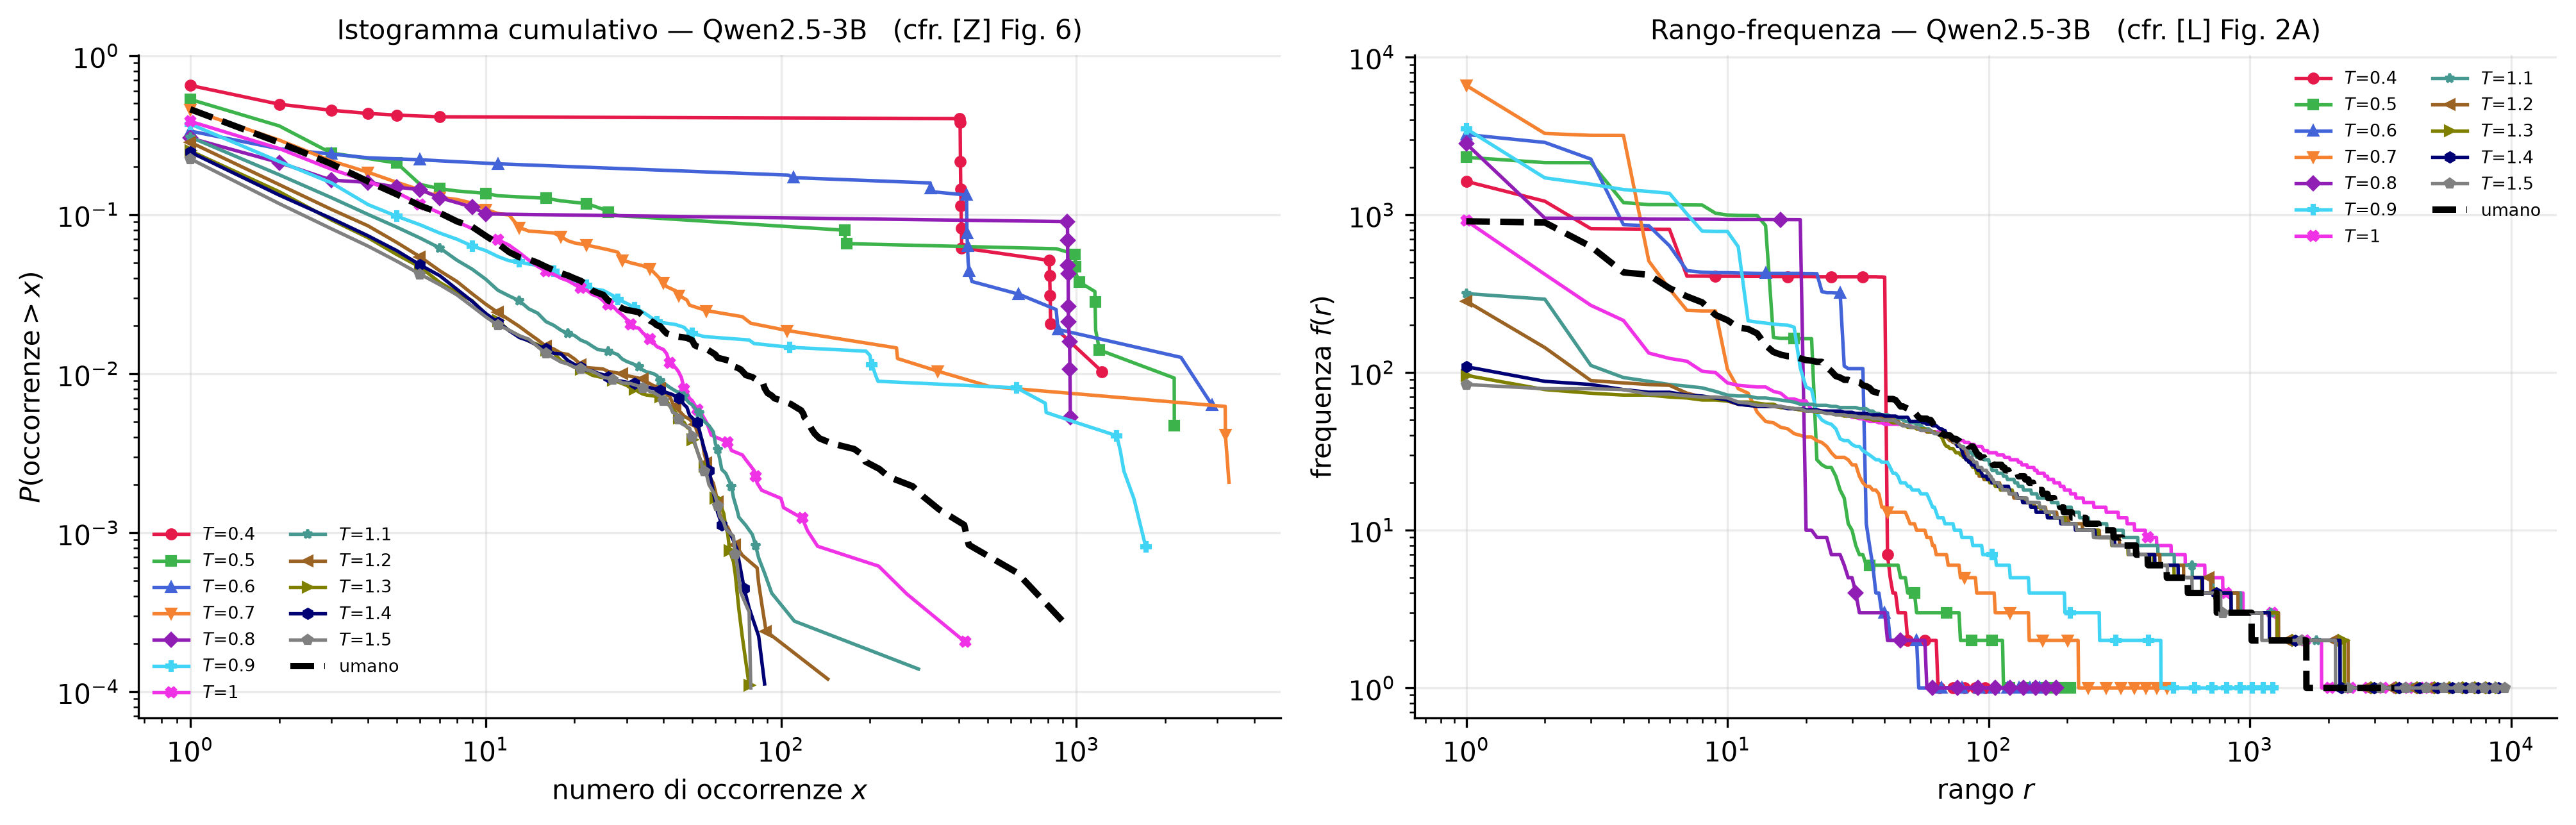
\includegraphics[width=\textwidth]{figure/cap4_zipf_cumulativo_Qwen25_3B.png}
  \caption{Istogrammi cumulativi delle frequenze dei token per il modello
  Qwen2.5-3B, una curva per temperatura. A bassa temperatura la curva è quasi
  verticale, perché pochi token coprono l'intero documento; ad alta temperatura
  è quasi orizzontale, perché quasi ogni token compare una volta sola. Solo
  nella regione intermedia la curva si avvicina alla retta che in coordinate
  bilogaritmiche corrisponde a una legge di potenza.}
  \label{fig:zipf-cum}
\end{figure}

L'esponente da solo non basta a descrivere questo comportamento, ed è la ragione
per cui nel §\ref{sec:zipf} è stato introdotto il MAPE: una curva può avere la
pendenza corretta e una curvatura marcata, e in tal caso l'esponente stimato non
descrive nulla. La Figura~\ref{fig:zipf-vs-T} riporta entrambe le quantità in
funzione della temperatura.

\begin{figure}[htbp]
  \centering
  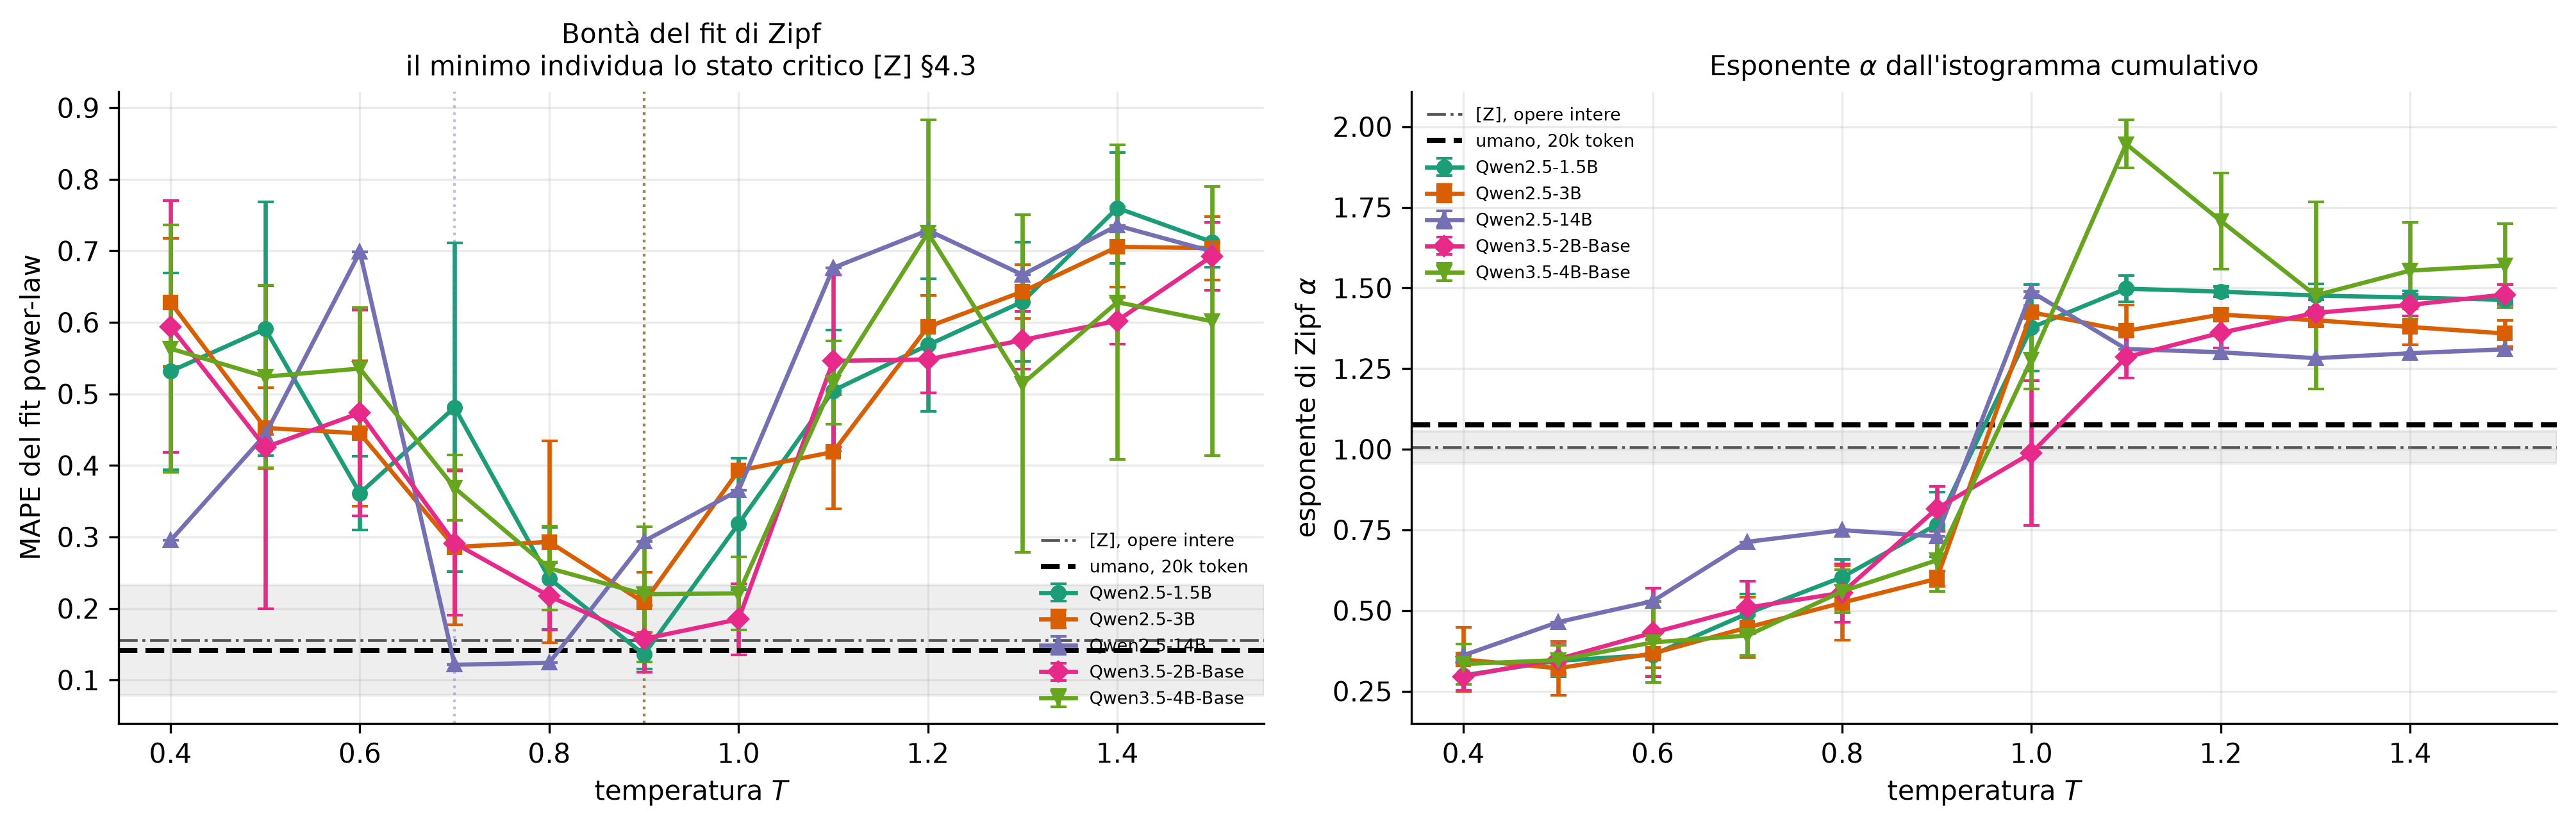
\includegraphics[width=\textwidth]{figure/cap4_zipf_vs_T.png}
  \caption{Bontà del fit e esponente della legge di Zipf in funzione della
  temperatura, per tutti e cinque i modelli. La banda grigia è il valore
  pubblicato su testi letterari interi, la linea nera tratteggiata la baseline
  umana misurata alla lunghezza di lavoro.}
  \label{fig:zipf-vs-T}
\end{figure}

Il MAPE ha un minimo pronunciato, che cade a $T = 0.9$ per quattro modelli su
cinque e a $T = 0.7$ per il modello da 14 miliardi di parametri. È il
risultato centrale della sezione: esiste una temperatura alla quale la
distribuzione delle frequenze del testo generato è più vicina a una legge di
potenza, e ai due lati di essa l'aderenza peggiora rapidamente.

Al minimo il MAPE del modello esemplare vale $0.208$. I due termini di
riferimento sono la baseline umana misurata alla stessa lunghezza, che vale
$0.141$, e il valore $0.156 \pm 0.077$ che~\cite{mikhaylovskiy2025zipf} riporta
su un corpus di sei opere letterarie in cinque lingue. Che i due riferimenti
umani cadano tanto vicini è una verifica indipendente della taratura della
baseline: sono ottenuti con tokenizzatori diversi, su testi diversi e di
lunghezza diversa, e la deriva documentata nella
Figura~\ref{fig:dimensione-finita} non rendeva scontato l'accordo.

Il valore del modello va letto contro tre metri diversi, e il giudizio che se ne
ricava non è lo stesso. Rispetto al modello stesso, $0.208$ è un risultato
netto: alle due estremità dell'intervallo lo stesso modello dà $0.628$ e
$0.704$, cioè un errore di fit tre volte più grande. Rispetto al testo umano è
invece una mezza vittoria: $0.208$ è circa una volta e mezza $0.141$, e resta
dentro la banda pubblicata solo perché quella banda è larga, sfiorandone il
margine superiore $0.233$. Rispetto agli altri modelli, infine, è un risultato
mediocre. La Tabella~\ref{tab:mape-minimi} riporta i cinque minimi: due modelli
scendono sotto il valore umano e un terzo vi si accosta, con $0.158$ contro
$0.141$, mentre il modello esemplare e il Qwen3.5-4B restano sopra.

\begin{table}[htbp]
\centering
\small
\begin{tabular}{@{}lrr@{}}
\toprule
Modello & $T$ del minimo & MAPE al minimo \\
\midrule
Qwen2.5-14B      & 0.7 & 0.121 \\
Qwen2.5-1.5B     & 0.9 & 0.136 \\
Qwen3.5-2B-Base  & 0.9 & 0.158 \\
Qwen2.5-3B       & 0.9 & 0.208 \\
Qwen3.5-4B-Base  & 0.9 & 0.220 \\
\midrule
testo umano      & --- & 0.141 \\
\bottomrule
\end{tabular}
\caption{Valore minimo del MAPE e temperatura alla quale viene raggiunto, per
ciascun modello, con la baseline umana misurata alla stessa lunghezza. Il
minimo esiste per tutti e cinque, ma solo tre modelli lo portano al livello del
testo umano o sotto. La riga del Qwen2.5-14B è ricavata da un solo campione per
temperatura e va letta con la cautela discussa nel testo.}
\label{tab:mape-minimi}
\end{table}

La prima riga della tabella richiede una precauzione. Il Qwen2.5-14B è l'unico
modello con un solo campione per temperatura, contro i tre o cinque degli altri,
e la sua curva del MAPE non è regolare da nessuno dei due lati del minimo: vale
$0.295$ a $T = 0.4$, sale a $0.698$ a $T = 0.6$ e scende a $0.121$ a $T = 0.7$,
cioè peggiora di un fattore due e migliora di un fattore sei in due passi
consecutivi. Negli altri quattro modelli la dispersione fra campioni alla stessa
temperatura va da $0.046$ a $0.230$ attorno a $T = 0.7$, mentre la distanza fra
il minimo del 14B e il suo valore a $T = 0.9$ vale $0.173$: sta dentro
quell'intervallo. Con una sola realizzazione la posizione del minimo non è
risolvibile, e il valore $T = 0.7$ va letto come compatibile con il $T = 0.9$
degli altri quattro anziché come uno spostamento reale. La stessa cautela vale
per la profondità: $0.121$ è il minimo più basso dei cinque ed è anche il meno
affidabile, mentre il $0.136$ del Qwen2.5-1.5B poggia su cinque campioni con
dispersione $0.020$ ed è l'unico caso in cui il primato sul testo umano è
sostenuto da repliche.

La posizione del minimo va confrontata con quella riportata nella fonte.
In~\cite{mikhaylovskiy2025zipf} il minimo del MAPE cade fra $t = 1.0$ e
$t = 1.2$ per tutti i modelli tranne i Llama più grandi, mentre qui cade a
$T = 0.9$ per quattro modelli su cinque. Lo scarto è nella direzione prevista
dall'effetto del prompt descritto nel §\ref{sec:protocollo}, che abbassa
l'errore del fit soprattutto alle basse temperature e sposta quindi il minimo
verso sinistra.

Ne segue una distinzione che vale per tutto il seguito. L'esistenza
di una temperatura ottimale è un fatto generale, comune a tutti e cinque i
modelli; la qualità dell'ottimo, cioè quanto il testo generato in quel punto
somigli davvero a un testo umano, varia da modello a modello e non è garantita.
Il modello scelto come esemplare non è fra quelli che ci riescono, e i grafici
del corpo del capitolo vanno letti tenendolo presente.

L'esponente $\alpha$ racconta la stessa storia da un'altra angolazione. Per il
modello esemplare passa da $0.35$ a $T = 0.4$, valore che corrisponde a una
distribuzione dominata da pochissimi tipi, a $1.36$ a $T = 1.5$, dove più di tre
quarti dei tipi compaiono una volta sola.\footnote{Un tipo che compare una sola
volta nel testo si dice \emph{hapax}. Gli hapax sono normalmente la maggioranza
dei tipi ma una piccola parte delle occorrenze: nella baseline umana usata qui
sono il $54\%$ dei tipi e il $10\%$ dei token, mentre a $T = 1.5$ il modello
esemplare arriva al $77\%$ dei tipi e al $37\%$ dei token.} La transizione non è
graduale: fra $T = 0.9$ e $T = 1.0$ l'esponente salta da $0.60$ a $1.43$,
attraversando in un solo passo il valore umano $1.076$, per poi assestarsi
attorno a $1.4$ senza più avvicinarvisi.

% ---------------------------------------------------------------------
\section{Legge di Heaps e descrittore \texorpdfstring{$R$}{R}}
\label{sec:heaps-risultati}

Le curve di crescita del vocabolario rendono immediatamente evidente perché il
§\ref{sec:heaps} abbia dovuto introdurre un descrittore alternativo all'esponente di
Heaps.

\begin{figure}[htbp]
  \centering
  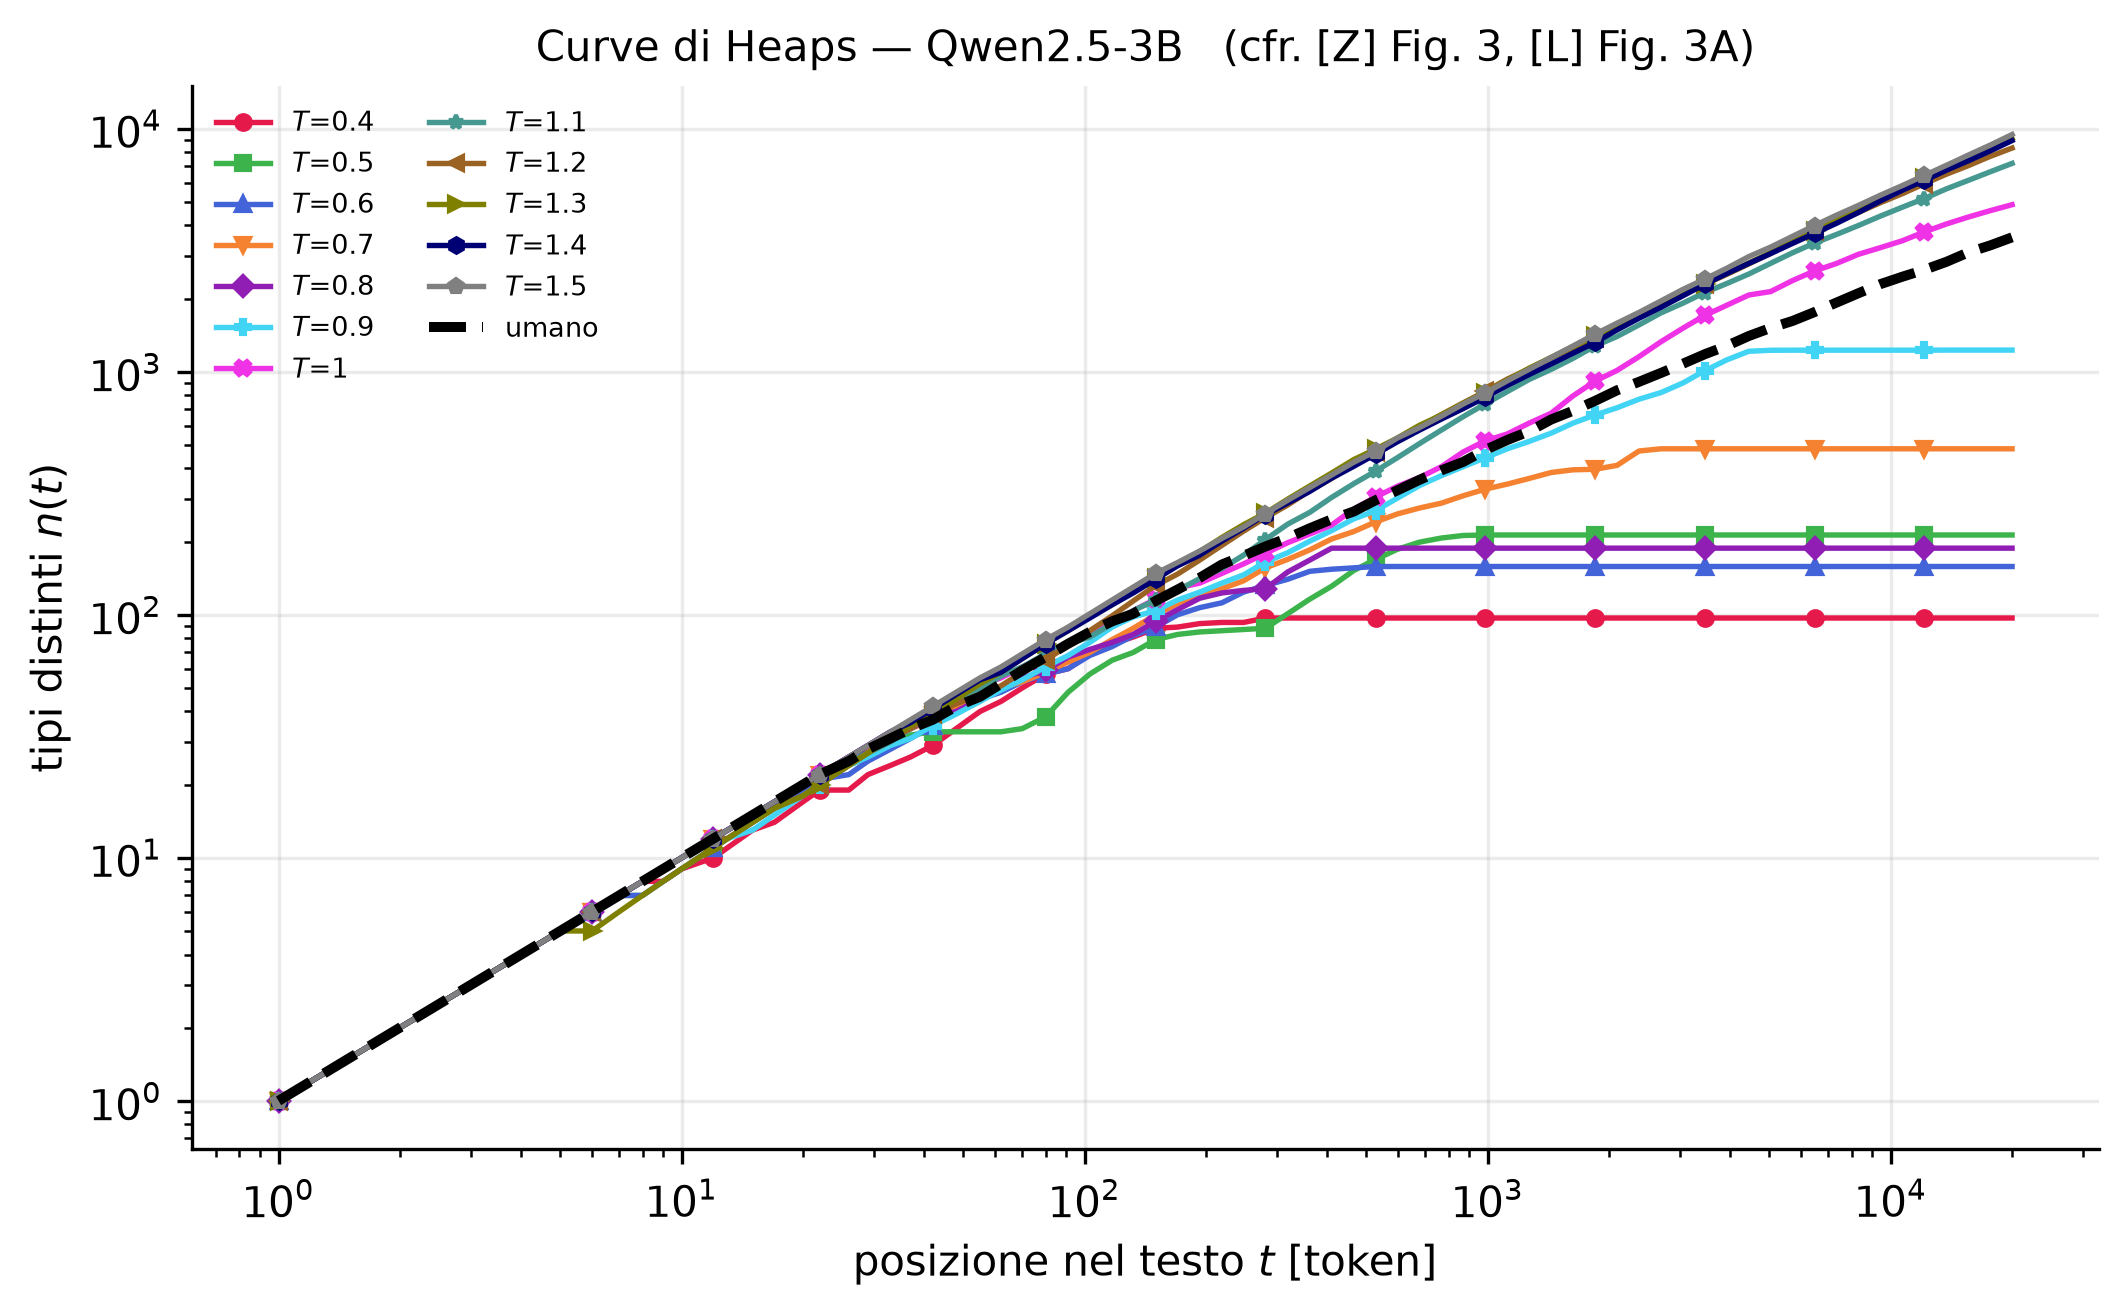
\includegraphics[width=0.86\textwidth]{figure/cap4_heaps_curve_Qwen25_3B.png}
  \caption{Crescita del vocabolario per il modello Qwen2.5-3B. Alle temperature
  basse la curva si appiattisce dopo poche migliaia di token: il modello ha
  smesso di produrre tipi nuovi. Alle temperature alte cresce quasi linearmente.
  In nessuno dei due casi la curva è una legge di potenza, e stimarne
  l'esponente restituisce un numero privo di contenuto.}
  \label{fig:heaps-curve}
\end{figure}

La Figura~\ref{fig:heaps-R} riporta il descrittore $R$, l'esponente $\gamma_H$
e il rapporto fra tipi e occorrenze in funzione della temperatura. I tre
andamenti sono concordi: per il modello esemplare $\gamma_H$ passa da $0.001$
a $T = 0.4$, dove la curva è piatta e il vocabolario non cresce affatto, a
$0.806$ a $T = 1.5$, attraversando il valore umano $0.668$ poco sopra $T =
0.9$. Il descrittore $R$ passa da $0.003$ a $0.688$ e incrocia il valore umano
$0.507$ attorno a $T = 1.05$.

Il terzo pannello riporta la quantità più elementare delle tre, il rapporto fra
il numero di tipi distinti e il numero di occorrenze, e serve da controllo sulle
altre due. A differenza di $\gamma_H$ e di $R$ non richiede alcun fit né alcuna
partizione del documento, quindi non può essere alterato da un modello mal
specificato: se le tre curve concordano, l'andamento non è un artefatto della
procedura di stima. Per il modello esemplare passa da $0.007$ a $T = 0.4$ a
$0.474$ a $T = 1.5$, e attraversa il valore umano $0.179$ fra $T = 0.9$ e
$T = 1.0$, cioè nello stesso punto delle altre due misure. Il pannello mostra
però anche in che senso l'accordo con il testo umano sia solo locale: sopra
$T = 1.1$ il rapporto supera il doppio del valore umano e continua a crescere,
mentre $\gamma_H$ resta stabile attorno a $0.8$. Le due misure smettono di dire
la stessa cosa non appena il vocabolario si allarga oltre quello di un romanzo.

\begin{figure}[htbp]
  \centering
  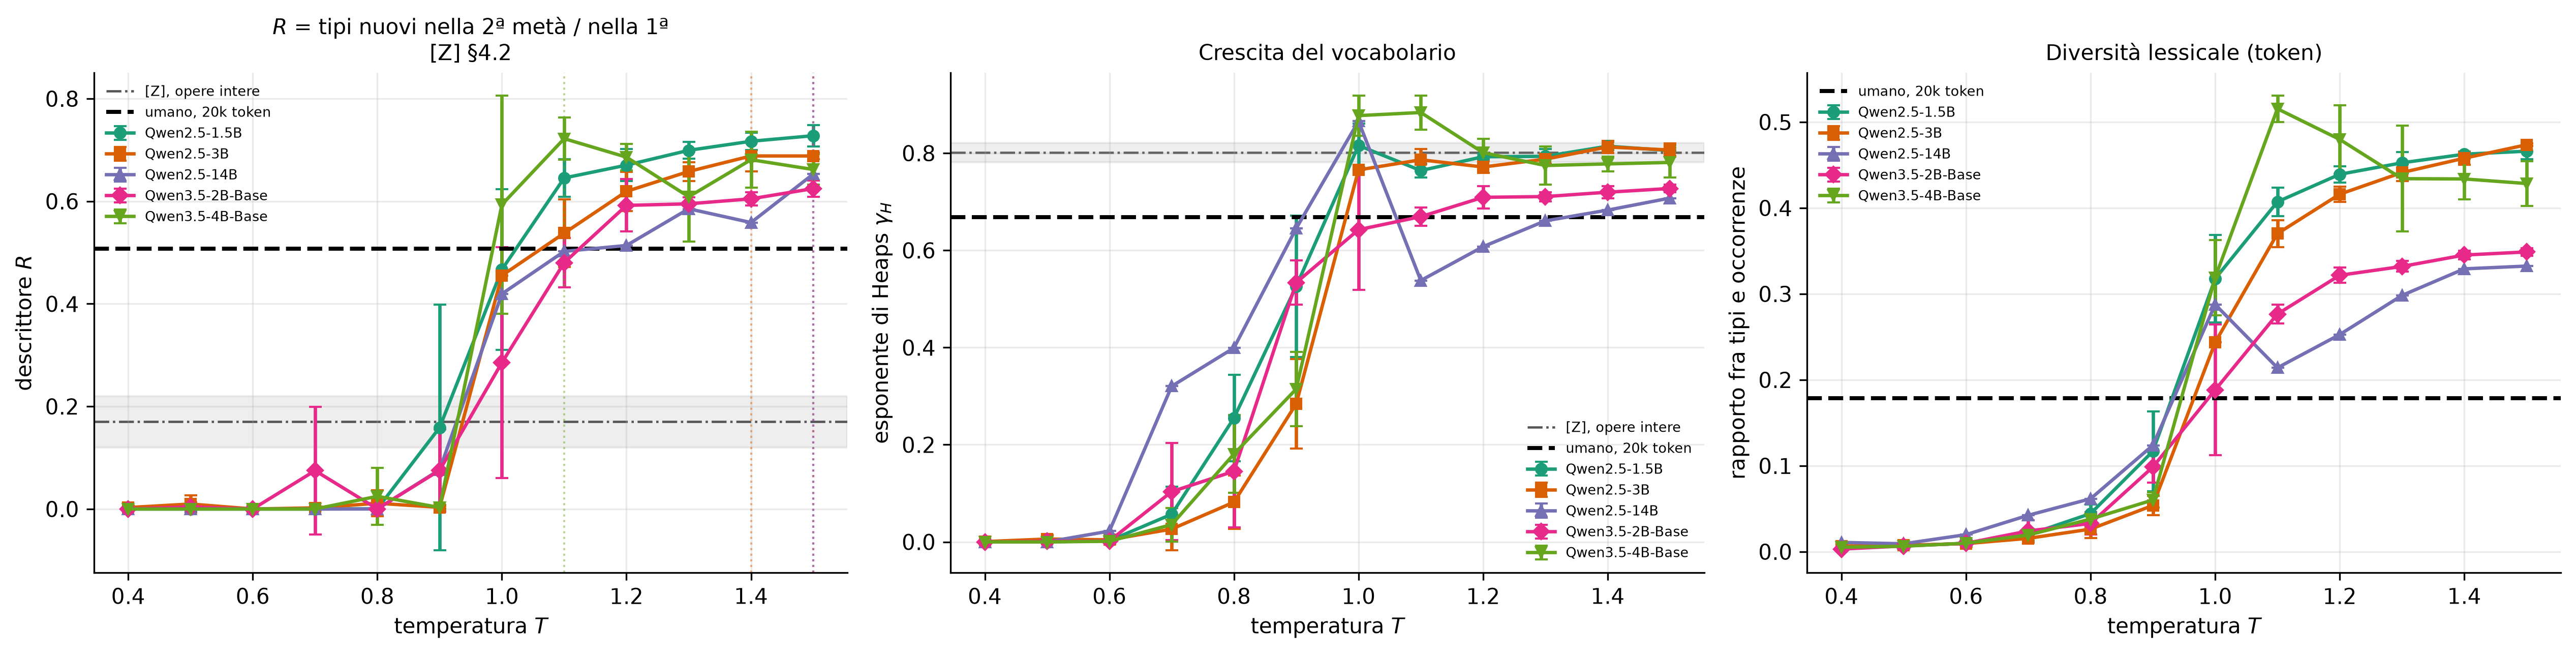
\includegraphics[width=\textwidth]{figure/cap4_heaps_R_vs_T.png}
  \caption{Descrittore $R$, esponente di Heaps e rapporto fra tipi e occorrenze
  in funzione della temperatura. La banda grigia riporta i valori pubblicati su
  opere intere, che per le ragioni discusse nel §\ref{sec:scelte} non sono un
  termine di confronto diretto.}
  \label{fig:heaps-R}
\end{figure}

% ---------------------------------------------------------------------
\section{Correlazioni a lungo raggio}
\label{sec:dfa-risultati}

Ogni documento viene convertito nella successione numerica definita nel
§\ref{sec:dfa}: ogni carattere è sostituito dal proprio rango di frequenza nel
documento, $1$ al più frequente, $2$ al secondo, e così via. È su quella
successione che si misura l'esponente della fluttuazione. Il detrending è
quadratico: il §\ref{sec:robustezza} documenta il confronto con quello lineare e
la ragione della scelta, cioè che alle basse temperature i documenti non sono
stazionari e un polinomio di primo grado non assorbe la deriva della
composizione dei caratteri. Il primo controllo riguarda il null model: la stessa
analisi condotta sui documenti rimescolati deve restituire un esponente pari a
$1/2$.


La Figura~\ref{fig:dfa} riporta le curve di fluttuazione e l'esponente in
funzione della temperatura. L'esponente ha un massimo a $T = 1.0$, dove vale
$0.719$ in media su tutti i modelli, superiore al valore umano di $0.579$;
decresce poi verso $0.53$ alle temperature più alte, avvicinandosi al valore del
rimescolamento senza raggiungerlo.

\begin{figure}[htbp]
  \centering
  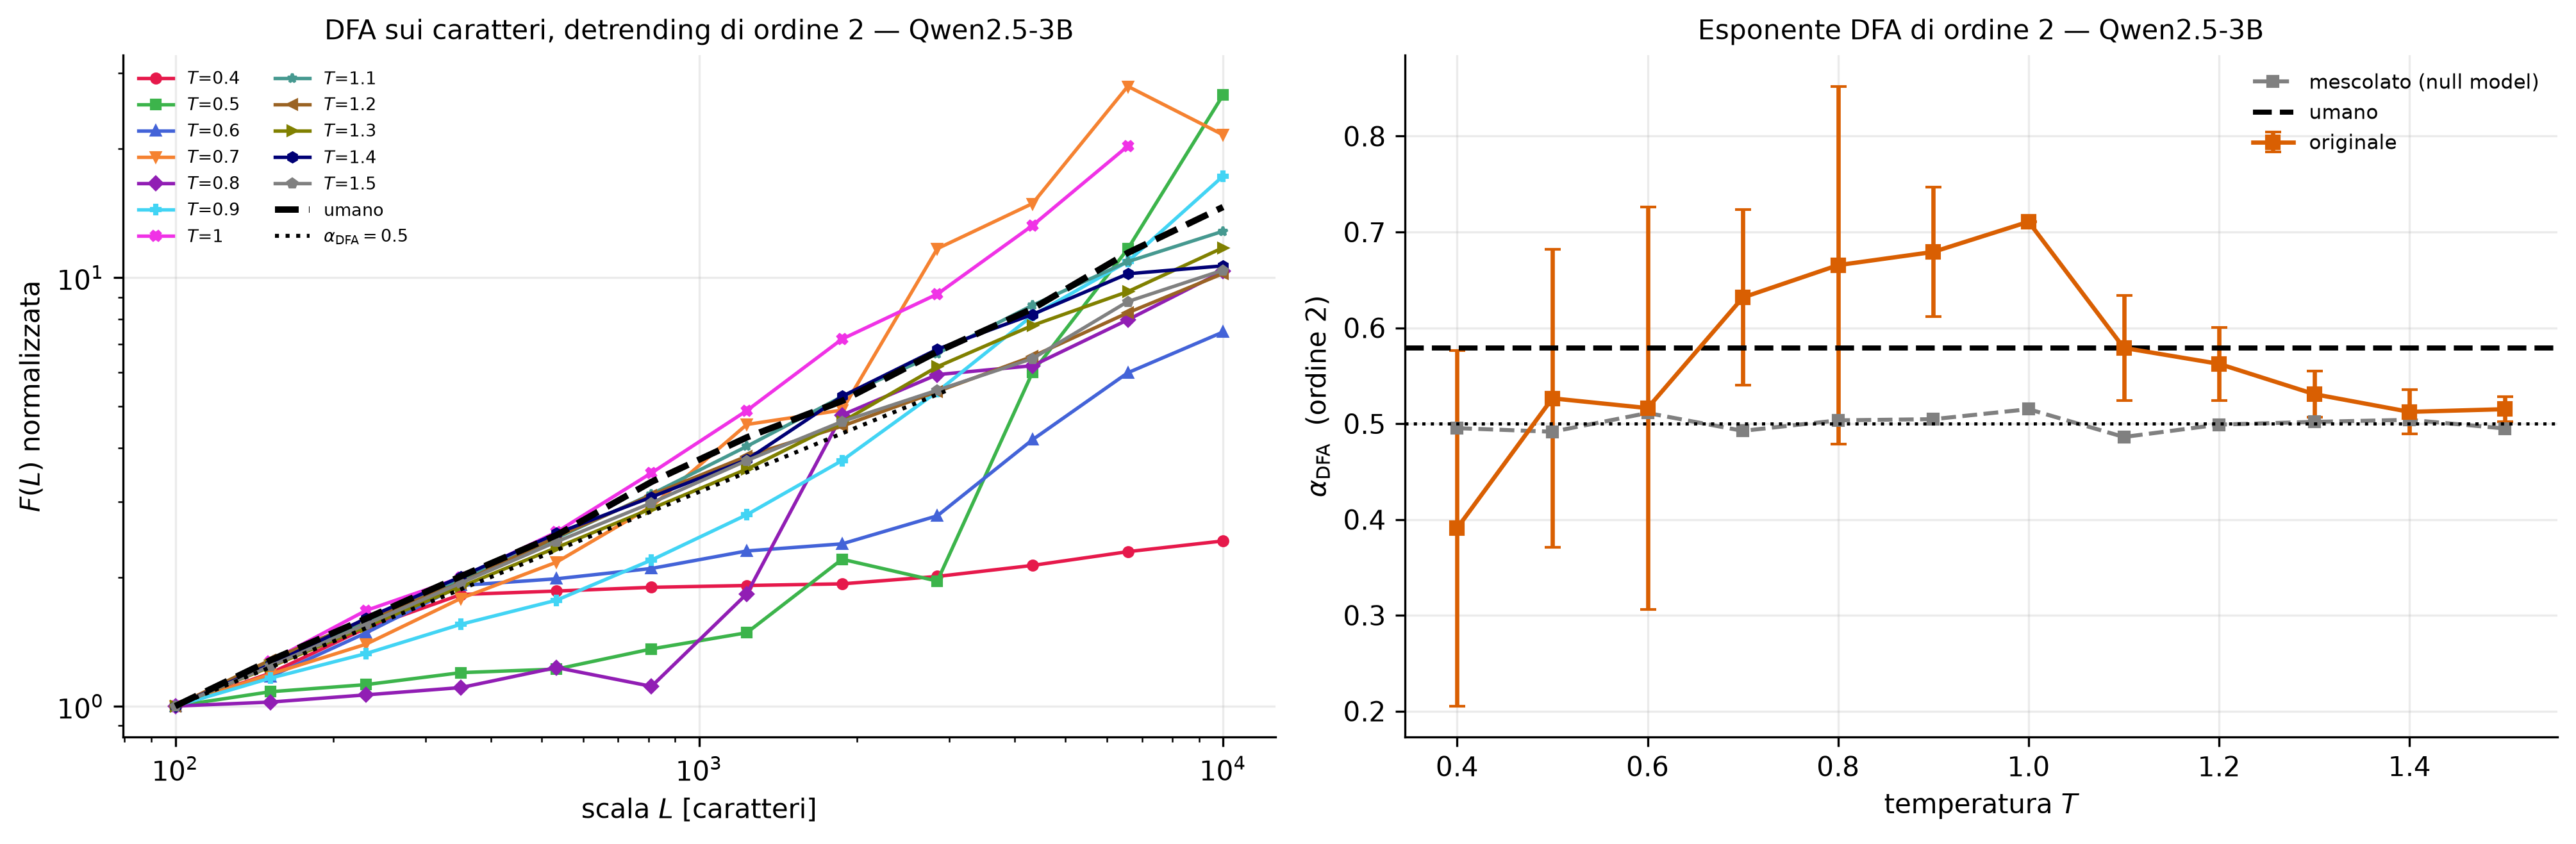
\includegraphics[width=\textwidth]{figure/cap4_dfa_Qwen25_3B_o2.png}
  \caption{Fluttuazione detrendizzata per il modello Qwen2.5-3B, con detrending
  quadratico. A sinistra $F(s)$ in funzione della scala, una curva per
  temperatura, con la pendenza di riferimento $\alpha_{\mathrm{DFA}} = 1/2$; a
  destra l'esponente in funzione della temperatura, con il null model
  rimescolato e la baseline umana.}
  \label{fig:dfa}
\end{figure}

\paragraph{La dispersione è il vero segnale.}
Il valore medio dell'esponente nasconde il fenomeno più informativo, ed è un
fenomeno già osservato: sulle reti LSTM~\cite{lippi2019} riporta che le stime
sui singoli campioni sono molto disperse attorno a $T = 0.5$ e strettamente
raccolte attorno alla media a $T = 1.0$. Gli stessi dati mostrano qui lo stesso
comportamento su architetture transformer. La deviazione standard fra documenti
passa da $0.219$ a $T = 0.4$ a $0.022$ a $T = 1.4$: alle basse temperature la
stima è dieci volte più dispersa. A $T = 0.4$ i cinque documenti del modello
esemplare danno esponenti compresi fra $0.16$ e $0.66$, cioè coprono
l'intervallo fra la saturazione e il valore umano; sull'insieme dei cinque
modelli l'escursione va da $0.07$ a $0.89$.

Questo comportamento è coerente con il caso limite discusso nel
§\ref{sec:ponte}. Quando il testo entra in un ciclo di ripetizione, il profilo
cumulato oscilla invece di allontanarsi dall'origine e la fluttuazione satura:
l'esponente crolla. Il crollo dipende però dalla lunghezza del ciclo rispetto
alle scale analizzate, che varia da documento a documento, e non tutti i testi
ripetitivi lo manifestano.

I dati permettono di precisare la relazione, che è a senso unico. Tutti e
diciannove i documenti con $\alpha_{\mathrm{DFA}} < 0.3$ si trovano a
$T \le 0.6$ e hanno una quota media di 8-grammi ripetuti pari a $0.984$: un
esponente collassato implica dunque ripetizione conclamata. Il viceversa non
vale: fra gli 82 documenti con quota di 8-grammi ripetuti superiore a $0.9$,
soltanto 33 hanno un esponente inferiore a $1/2$, e la correlazione di rango fra
le due quantità non è significativa
($\rho = +0.03$, $p = 0.61$). La ripetizione è quindi condizione necessaria ma
non sufficiente al collasso dell'esponente.

Ne segue una conseguenza metodologica. Alle basse temperature
$\alpha_{\mathrm{DFA}}$ non è un indicatore affidabile di correlazione a lungo
raggio, né lo è il suo valore medio; è la sua dispersione a segnalare il regime.
Il controllo sull'ordine del detrending riportato nel §\ref{sec:robustezza}
punta nella stessa direzione, poiché lo scarto fra i due ordini è massimo
proprio nell'intervallo $T \in [0.5, 0.8]$ e trascurabile altrove.

% ---------------------------------------------------------------------
\section{Entropia, divergenza dal testo umano e plagio}
\label{sec:entropia-risultati}

Le sezioni precedenti confrontano il testo generato con quello umano una misura
alla volta. La divergenza di Kullback--Leibler introdotta nel
§\ref{sec:crossparsing} permette invece un confronto diretto fra i due testi,
senza passare per un descrittore intermedio, ed è per questa ragione il criterio
più stringente del capitolo: non dipende da soglie teoriche né dalla scelta di
quale proprietà misurare.


La divergenza ha un minimo netto, che cade a $T = 0.9$ per quattro modelli su
cinque e a $T = 1.0$ per Qwen3.5-4B-Base. Nessuna delle \num{242} stime risulta
negativa, il che conferma sui dati reali la proprietà dello stimatore verificata
nel §\ref{sec:validazione}.

Il valore al minimo varia molto fra i modelli: $0.096$ bit per carattere per il
modello da 14 miliardi di parametri, $0.232$ e $0.245$ per i due Qwen3.5,
$0.321$ per il modello da 1.5 miliardi e $0.914$ per quello da 3 miliardi. La
posizione del minimo è dunque comune, la sua profondità no: fra il modello che
si avvicina di più al testo umano e quello che ci riesce meno corre quasi un
fattore dieci. La profondità non segue però la dimensione. La correlazione di
rango con il numero di parametri vale $\rho = -0.50$ con $p = 0.39$ su cinque
modelli, e il valore peggiore appartiene al modello da 3 miliardi anziché al più
piccolo: quanto un modello si avvicini al testo umano nel proprio punto migliore
è una proprietà del singolo modello, non della sua scala, almeno con la potenza
statistica qui disponibile. Vale inoltre la cautela imposta dal
§\ref{sec:robustezza}, poiché il modello da 14 miliardi dispone di un solo
campione per temperatura e il suo valore non è corredato da una stima della
dispersione.

L'entropia stimata per compressione mostra la transizione in modo ancora più
brusco. Per il modello esemplare la mediana vale $0.001$ bit per carattere
fino a $T = 0.8$, perché il testo ripetitivo è essenzialmente incomprimibile
oltre la prima occorrenza del ciclo e non trasporta informazione; sale poi a
$0.332$ in media a $T = 0.9$ e supera $4$ da $T = 1.0$ in poi, contro i $2.23$
del testo umano. Fra $T = 0.6$ e $T = 0.9$ la media si stacca dalla mediana
perché un documento per temperatura esce dal ciclo prima degli altri, e il
valore isolato di $5.77$ che il modello esemplare raggiunge a $T = 1.0$
proviene dall'unico documento sopravvissuto a quella temperatura: è la stessa
dispersione descritta nel §\ref{sec:dfa-risultati}, e conferma che nel regime
periodico il valore medio non descrive alcun documento. Il passaggio dal
regime a entropia trascurabile a quello a entropia superiore a quella umana si
consuma comunque entro due passi di temperatura.

% ---------------------------------------------------------------------
\section{Struttura misurata per compressione}
\label{sec:compressione-risultati}

Le misure basate su compressione del §\ref{sec:compressione} non richiedono di
scegliere un'unità di analisi né di stimare un esponente: operano direttamente
sui byte del testo. Costituiscono quindi un controllo indipendente da tutte le
scelte metodologiche discusse finora.

\begin{figure}[htbp]
  \centering
  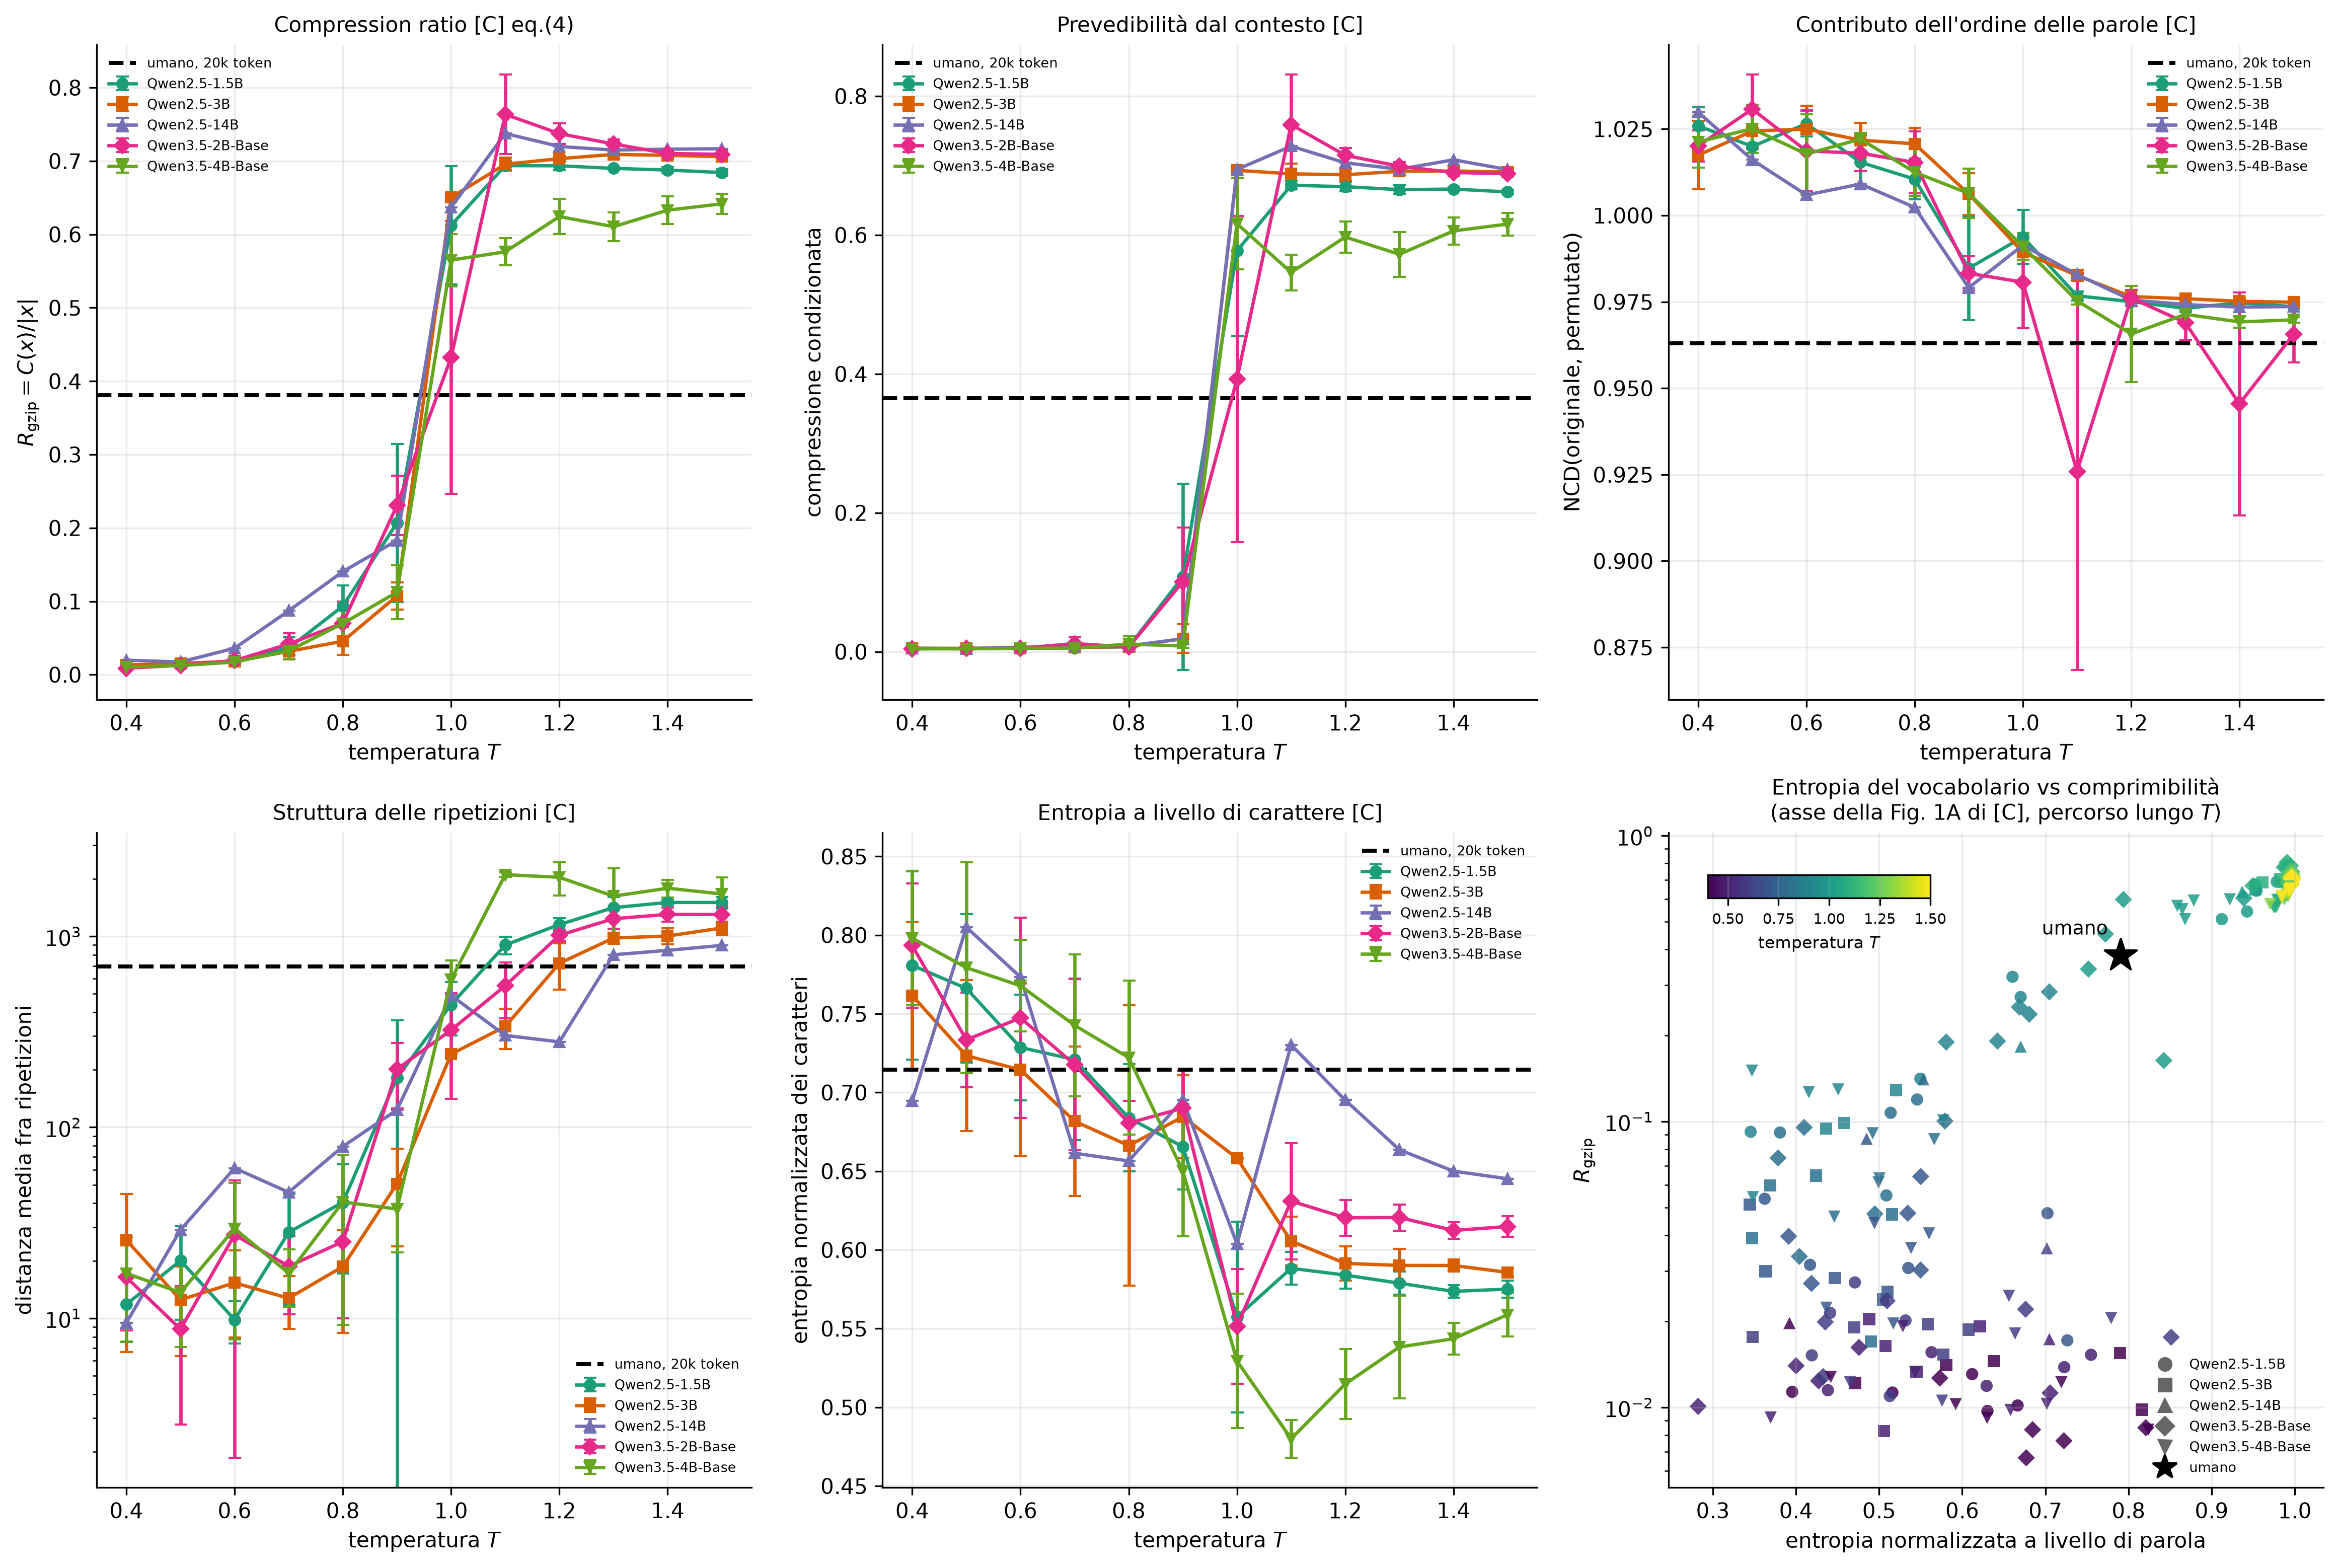
\includegraphics[width=\textwidth]{figure/cap4_compressione.png}
  \caption{Sei misure basate su compressione. Le prime cinque sono riportate in
  funzione della temperatura; l'ultima, in basso a destra, riporta il rapporto
  di compressione contro
  l'entropia normalizzata a livello di parola: è il piano della Figura~1A
  di~\cite{hadad2026}, percorso qui facendo variare la temperatura, con il testo
  umano segnato da una stella. In quel pannello il colore codifica la
  temperatura e la forma del marcatore il modello, e la scala verticale è
  logaritmica.}
  \label{fig:compressione}
\end{figure}

Il rapporto di compressione è la misura che separa i regimi in modo più netto di
tutte le altre. Per il modello esemplare passa da $0.013$ a $T = 0.4$ a $0.107$
a $T = 0.9$ e a $0.650$ a $T = 1.0$: un fattore cinquanta fra i due estremi, con
un salto di un fattore sei concentrato in un singolo passo di temperatura. Il
valore umano è $0.381$, e viene attraversato fra $T = 0.9$ e $T = 1.0$ come
tutte le altre misure del capitolo.

Il lavoro di~\cite{hadad2026} riporta che il testo generato è più regolare e
più comprimibile di quello umano, mentre qui il rapporto di compressione
supera il valore umano sopra $T = 1.0$. Le due osservazioni non sono in
contrasto, perché descrivono regioni diverse dello stesso asse: sotto la
transizione il testo generato è molto più comprimibile del testo umano,
$0.013$ contro $0.381$, ed è il regime in cui i modelli operano con le
impostazioni ordinarie; sopra la transizione la comprimibilità cade perché il
testo cessa di essere linguaggio, non perché acquisti struttura.

La compressione condizionata si comporta in modo analogo ma dice qualcosa di
diverso. Fino a $T = 0.9$ vale meno di $0.02$: la seconda metà del documento è
quasi interamente prevedibile dalla prima, come è ovvio in un testo che ripete
lo stesso ciclo. Da $T = 1.0$ sale a circa $0.69$, quasi il doppio del valore
umano $0.365$: la seconda metà è ora \emph{meno} prevedibile dalla prima di
quanto lo sia in un romanzo. Fra i due regimi non esiste una temperatura in cui
la predicibilità dal contesto assomigli a quella del testo umano.

Il salto oltre il valore umano non è una particolarità del modello esemplare. La
mediana su tutti e cinque i modelli passa da $0.015$ a $T = 0.9$ a $0.627$ a
$T = 1.0$, e il singolo modello che si avvicina di più al valore umano da sotto,
il Qwen3.5-2B-Base con $0.135$, lo scavalca comunque in un passo arrivando a
$0.430$. Nessuno dei cinque si ferma sul valore umano, ed è l'unica delle misure
di questo capitolo per cui ciò accade.

\paragraph{Il piano entropia--comprimibilità.}
Il pannello in basso a destra della Figura~\ref{fig:compressione} colloca i
documenti nel piano definito da~\cite{hadad2026}, percorso qui da un modello
reale al variare di un solo parametro anziché da distribuzioni artificiali, con
il testo umano in posizione intermedia. L'asse verticale è logaritmico perché il rapporto di compressione
non si annulla mai: il valore più basso osservato è $0.0067$. Su un asse
lineare esteso fino a $0.81$, però, i 57 documenti che stanno fra $0.007$ e
$0.020$, quasi un quarto del totale, si sovrappongono tutti sulla linea dello
zero, e la loro struttura interna scompare. In scala logaritmica si vede
invece che occupano un intervallo di entropia molto ampio, da $0.28$ a $0.85$,
e la ragione è che le due grandezze misurano cose diverse. Il rapporto di
compressione dipende dalla ripetizione della sequenza: un testo che ripete
sempre lo stesso ciclo si comprime a poco più dell'un per cento della sua
dimensione, qualunque sia il numero di parole che il ciclo contiene.
L'entropia normalizzata dipende invece dalla forma della distribuzione delle
frequenze su quel vocabolario ridotto, che conta fra 37 e 235 tipi distinti.
Un ciclo lungo e vario e un ciclo corto e povero sono ugualmente comprimibili
ma hanno entropie molto diverse: da qui la dispersione orizzontale della
nuvola a bassa comprimibilità.

\paragraph{La lunghezza del ciclo, misurata.}
L'argomento appena esposto invoca una grandezza che le misure di questo capitolo
non contengono, la lunghezza del ciclo ripetuto, ed è quindi il caso di
misurarla. Sulla successione di parole di ciascun documento si cerca il più
piccolo sfasamento $L_{\mathrm{ciclo}}$ per cui l'accordo fra la parola in
posizione $i$ e quella in posizione $i - L_{\mathrm{ciclo}}$, calcolato sugli
ultimi venti giri, supera il novanta per cento. La finestra di verifica è locale
e commisurata al periodo candidato: su tutto il testo la prosa che precede il
ciclo diluirebbe la media, mentre su un suffisso lungo un ciclo che cambia
lentamente variante scende sotto soglia al proprio periodo e la supera a un
multiplo, restituendo un alias. La soglia è fissata al novanta e non al cento
per cento per tollerare i cicli non esattamente verbatim; l'accordo atteso per
caso in prosa inglese è circa $0.05$, quindi non vi sono falsi positivi.

Il criterio individua \num{113} documenti su \num{242}, e sono tutti a
$T \le 0.9$: la totalità fino a $T = 0.7$, il $95\%$ a $T = 0.8$, il $56\%$ a
$T = 0.9$ e nessuno da
$T = 1.0$ in poi. Coincidono con la nuvola a bassa comprimibilità: tutti e
cinquantasette i documenti con $R_{\mathrm{gzip}} < 0.02$ sono fra questi. Il
ciclo va da una sola parola a \num{248}, in caratteri da $9$ a \num{1127}, con
mediana di $16$ parole.

La Figura~\ref{fig:ciclo} riporta la relazione con le due grandezze del piano.
Con l'entropia di parola la correlazione di rango vale $\rho = +0.65$, e non è
un effetto della temperatura: calcolata fra documenti generati alla stessa
temperatura sale a $+0.69$, ed è positiva in tutti e sei i gruppi. Con il
rapporto di compressione, invece, non c'è relazione: $\rho = -0.15$ con
$p = 0.12$, e a temperatura fissata il segno si inverte, $+0.16$ con
$p = 0.11$. A parità di lunghezza del ciclo il rapporto di compressione varia di
un fattore compreso fra quattordici e ventisette.

Il meccanismo è quello anticipato sopra, e la misura lo rende esplicito: la
lunghezza del ciclo coincide quasi con il numero di tipi distinti che esso
contiene, $\rho = +0.84$, cosicché un ciclo corto concentra tutta la massa di
probabilità su poche parole e uno lungo la distribuisce. Gli estremi lo
mostrano nel modo più diretto: il ciclo più corto osservato è una sola parola,
ripetuta, con entropia $0.35$; il più lungo conta \num{248} parole e undici
tipi distinti, \emph{You are a bad father. You are a bad lover of children.
You are not to blame} con variazioni, con entropia $0.47$ e $R_{\mathrm{gzip}}
= 0.019$, cioè testo ancora ultracomprimibile. La lunghezza del ciclo spiega
dunque l'ordinamento lungo l'asse orizzontale del piano, non tutta la sua
dispersione: la regressione su $\log L_{\mathrm{ciclo}}$ rende conto del
$42\%$ della varianza dell'entropia.

\begin{figure}[htbp]
  \centering
  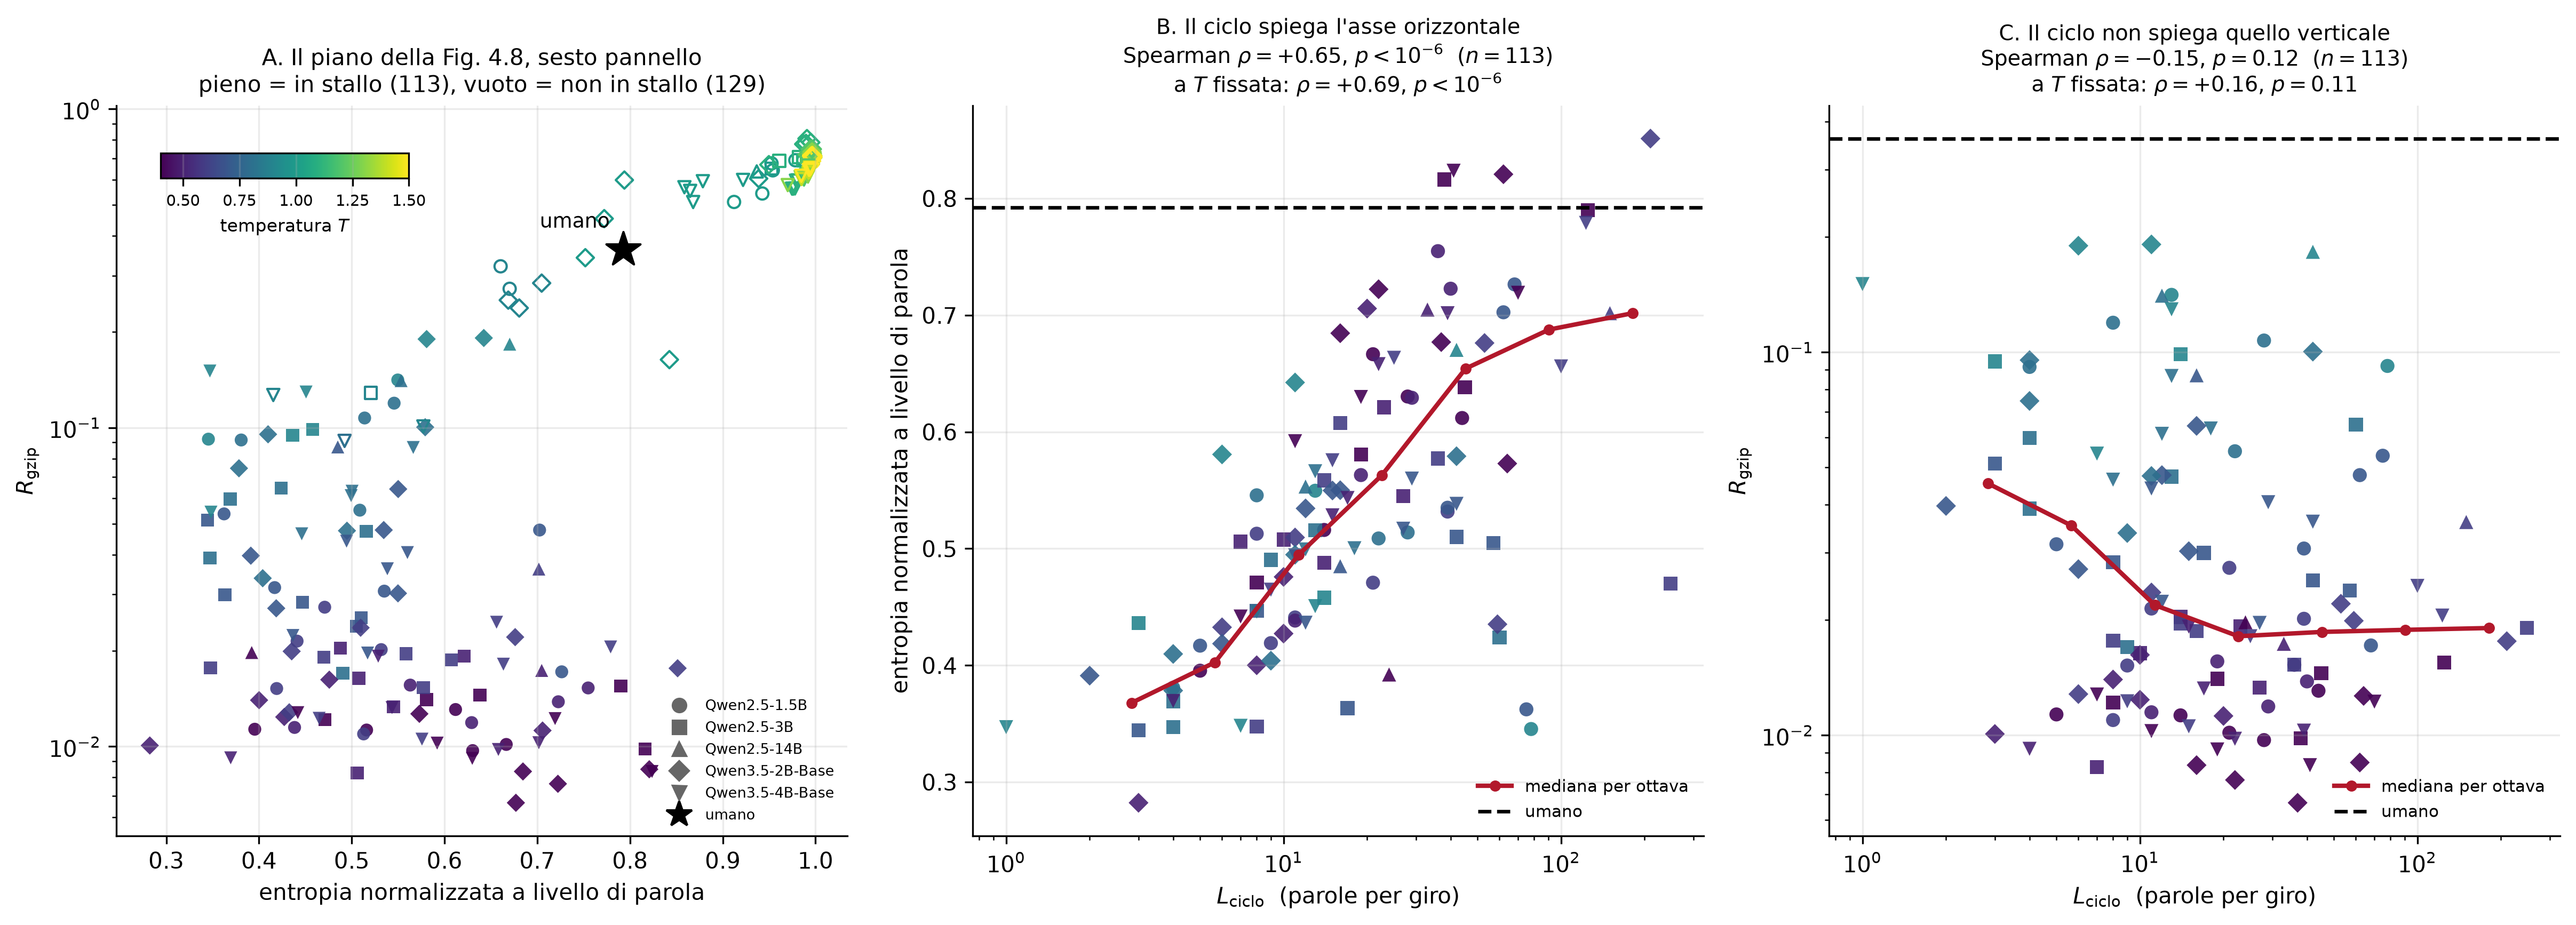
\includegraphics[width=\textwidth]{figure/cap4_ciclo_entropia.png}
  \caption{Lunghezza del ciclo ripetuto in fase di stallo. A: il piano
  entropia--comprimibilità della Figura~\ref{fig:compressione}, con i documenti
  in stallo a simbolo pieno e gli altri a simbolo vuoto; il colore codifica la
  temperatura e la forma il modello. B: entropia di parola contro lunghezza del
  ciclo, con la mediana per ottava. C: rapporto di compressione contro la stessa
  grandezza. La lunghezza del ciclo ordina l'asse orizzontale del piano e non
  quello verticale.}
  \label{fig:ciclo}
\end{figure}


% ---------------------------------------------------------------------
\section{Le tre fasi}
\label{sec:fasi-risultati}

Le misure precedenti descrivono il testo generato senza classificarlo. La regola
del §\ref{sec:tre-fasi} permette invece di assegnare ciascun documento a una
fase, e questa sezione ne riporta l'esito.

La traiettoria della~\eqref{eq:traiettoria} è costruita sui vettori GloVe a 100
dimensioni già impiegati nel §\ref{sec:token}, e l'autocorrelazione è calcolata
sui primi cento lag, misurati in parole. Il fit del GAPELMAPER usa invece un
intervallo più ampio, fino a 600 parole, perché distinguere una legge di potenza
da un esponenziale richiede più di una decade di distanze. Il livello di rumore
$\eta$ è stimato su una singola permutazione della traiettoria di ciascun
documento, con seme fissato.

Le due soglie della regola valgono $\kappa_{\min} = 0.50$ e $\Phi_{\min} = 3$.
La prima è deliberatamente permissiva: serve a escludere i documenti in cui meno
di metà delle parole ha un vettore, cioè quelli in cui la traiettoria è fatta per
lo più di zeri, e non a selezionare i documenti buoni. La seconda separa i due
gruppi in cui $\Phi$ effettivamente si distribuisce, e la sua posizione è poco
critica: come mostra la Figura~\ref{fig:transizioni}, fra la fase periodica e
quella successiva $\Phi$ cambia di due ordini di grandezza, cosicché qualunque
soglia compresa fra $1$ e $5$ produce la stessa classificazione. Il
§\ref{sec:tstar} riprende il punto trattando la fine della fase periodica come
uno degli otto criteri di temperatura critica.

La Figura~\ref{fig:acf} mostra come questa autocorrelazione cambia lungo lo
sweep. Fino a $T = 0.9$ la curva oscilla con periodo definito e ampiezza
prossima all'unità: il testo ripete un ciclo di parole, e a distanza pari a un
multiplo del ciclo ogni vettore ritrova sé stesso. Il periodo si accorcia al
crescere della temperatura, da dieci parole a $T = 0.5$ a circa tre a $T =
0.8$, mentre l'ampiezza scende da $0.98$ a $0.72$. Fra $T = 0.9$ e $T = 1.0$
la struttura periodica scompare del tutto: l'ampiezza cade a $0.036$ e la
curva diventa un decadimento monotono, senza più oscillazione. A $T = 1.3$
l'intera curva è contenuta nella banda di rumore stimata mescolando le parole
del documento, cioè non è distinguibile dal caso.

Il confronto con il testo umano chiarisce quanto entrambi i regimi siano
lontani dal linguaggio naturale. L'autocorrelazione del romanzo non è
periodica, con $\max\lvert\mathrm{FFT}\rvert$ pari a $1.16$, ben sotto la
soglia $3$, ma è nettamente sopra il livello di rumore su tutti i cento lag
esaminati, e il suo spettro decade in modo regolare invece di essere piatto.
Nessuna delle temperature campionate riproduce questa combinazione: sotto la
transizione la correlazione è troppo forte e periodica, sopra è assente.

\begin{figure}[htbp]
  \centering
  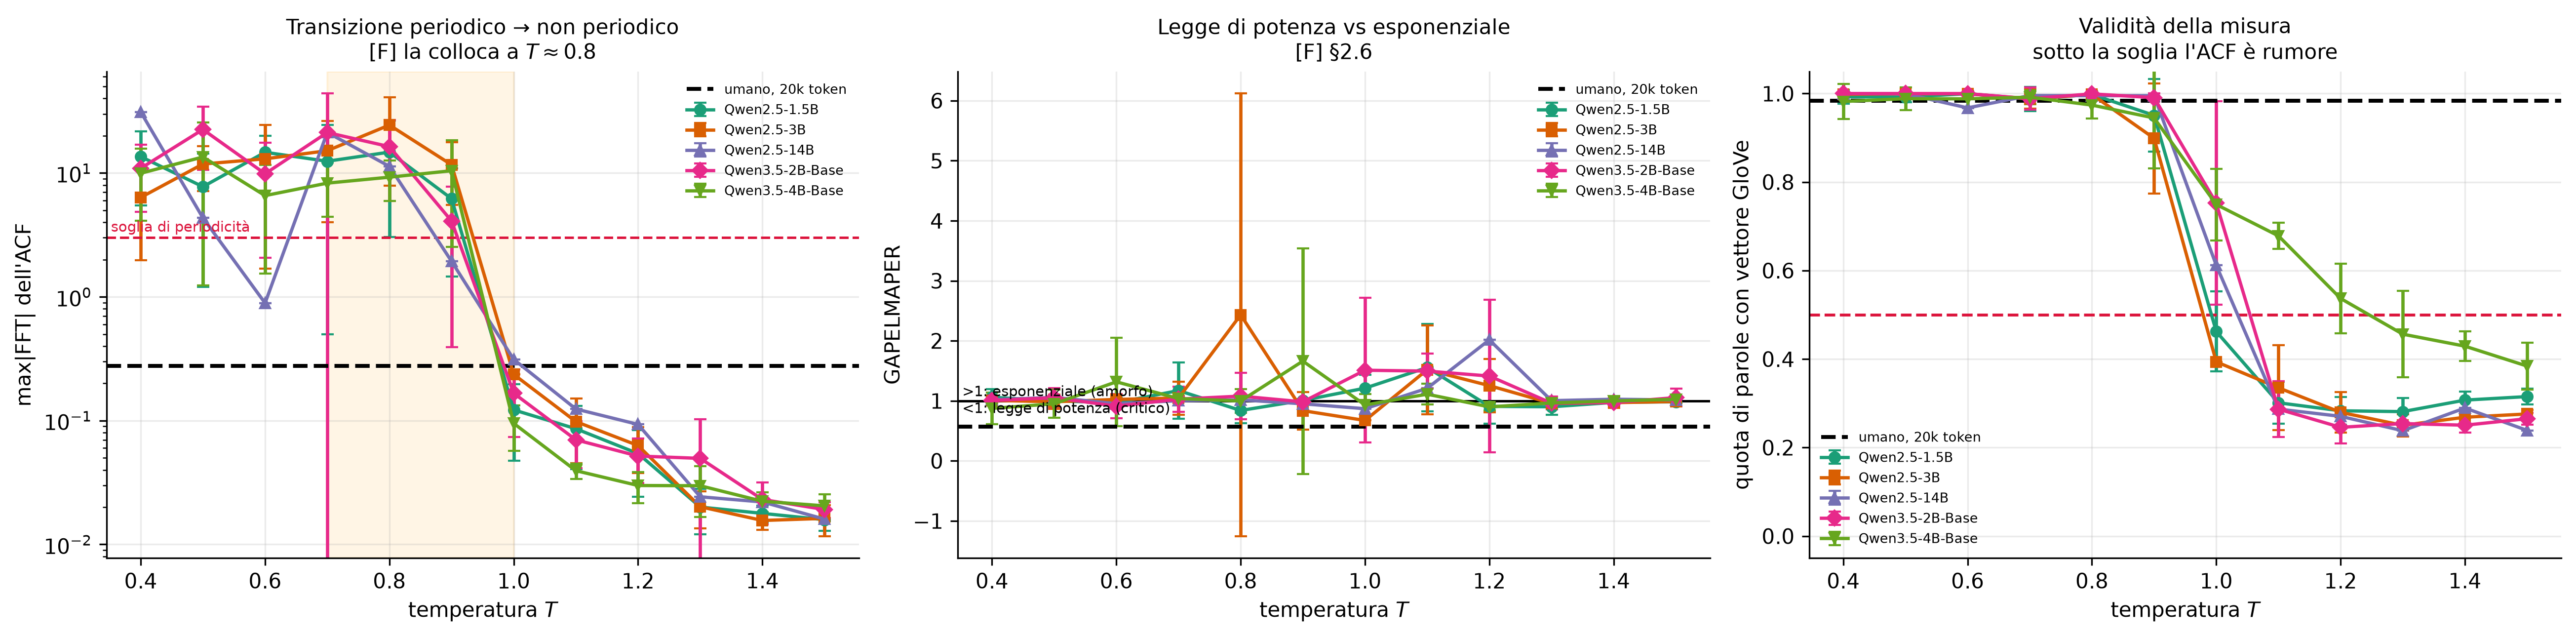
\includegraphics[width=\textwidth]{figure/cap4_transizioni_fase.png}
  \caption{Parametro di periodicità, GAPELMAPER e copertura degli embedding in
  funzione della temperatura. Il primo pannello è in scala logaritmica. Il terzo
  riporta la quota di parole dotate di un vettore, che è la condizione di
  validità delle altre due misure.}
  \label{fig:transizioni}
\end{figure}

\begin{figure}[htbp]
  \centering
  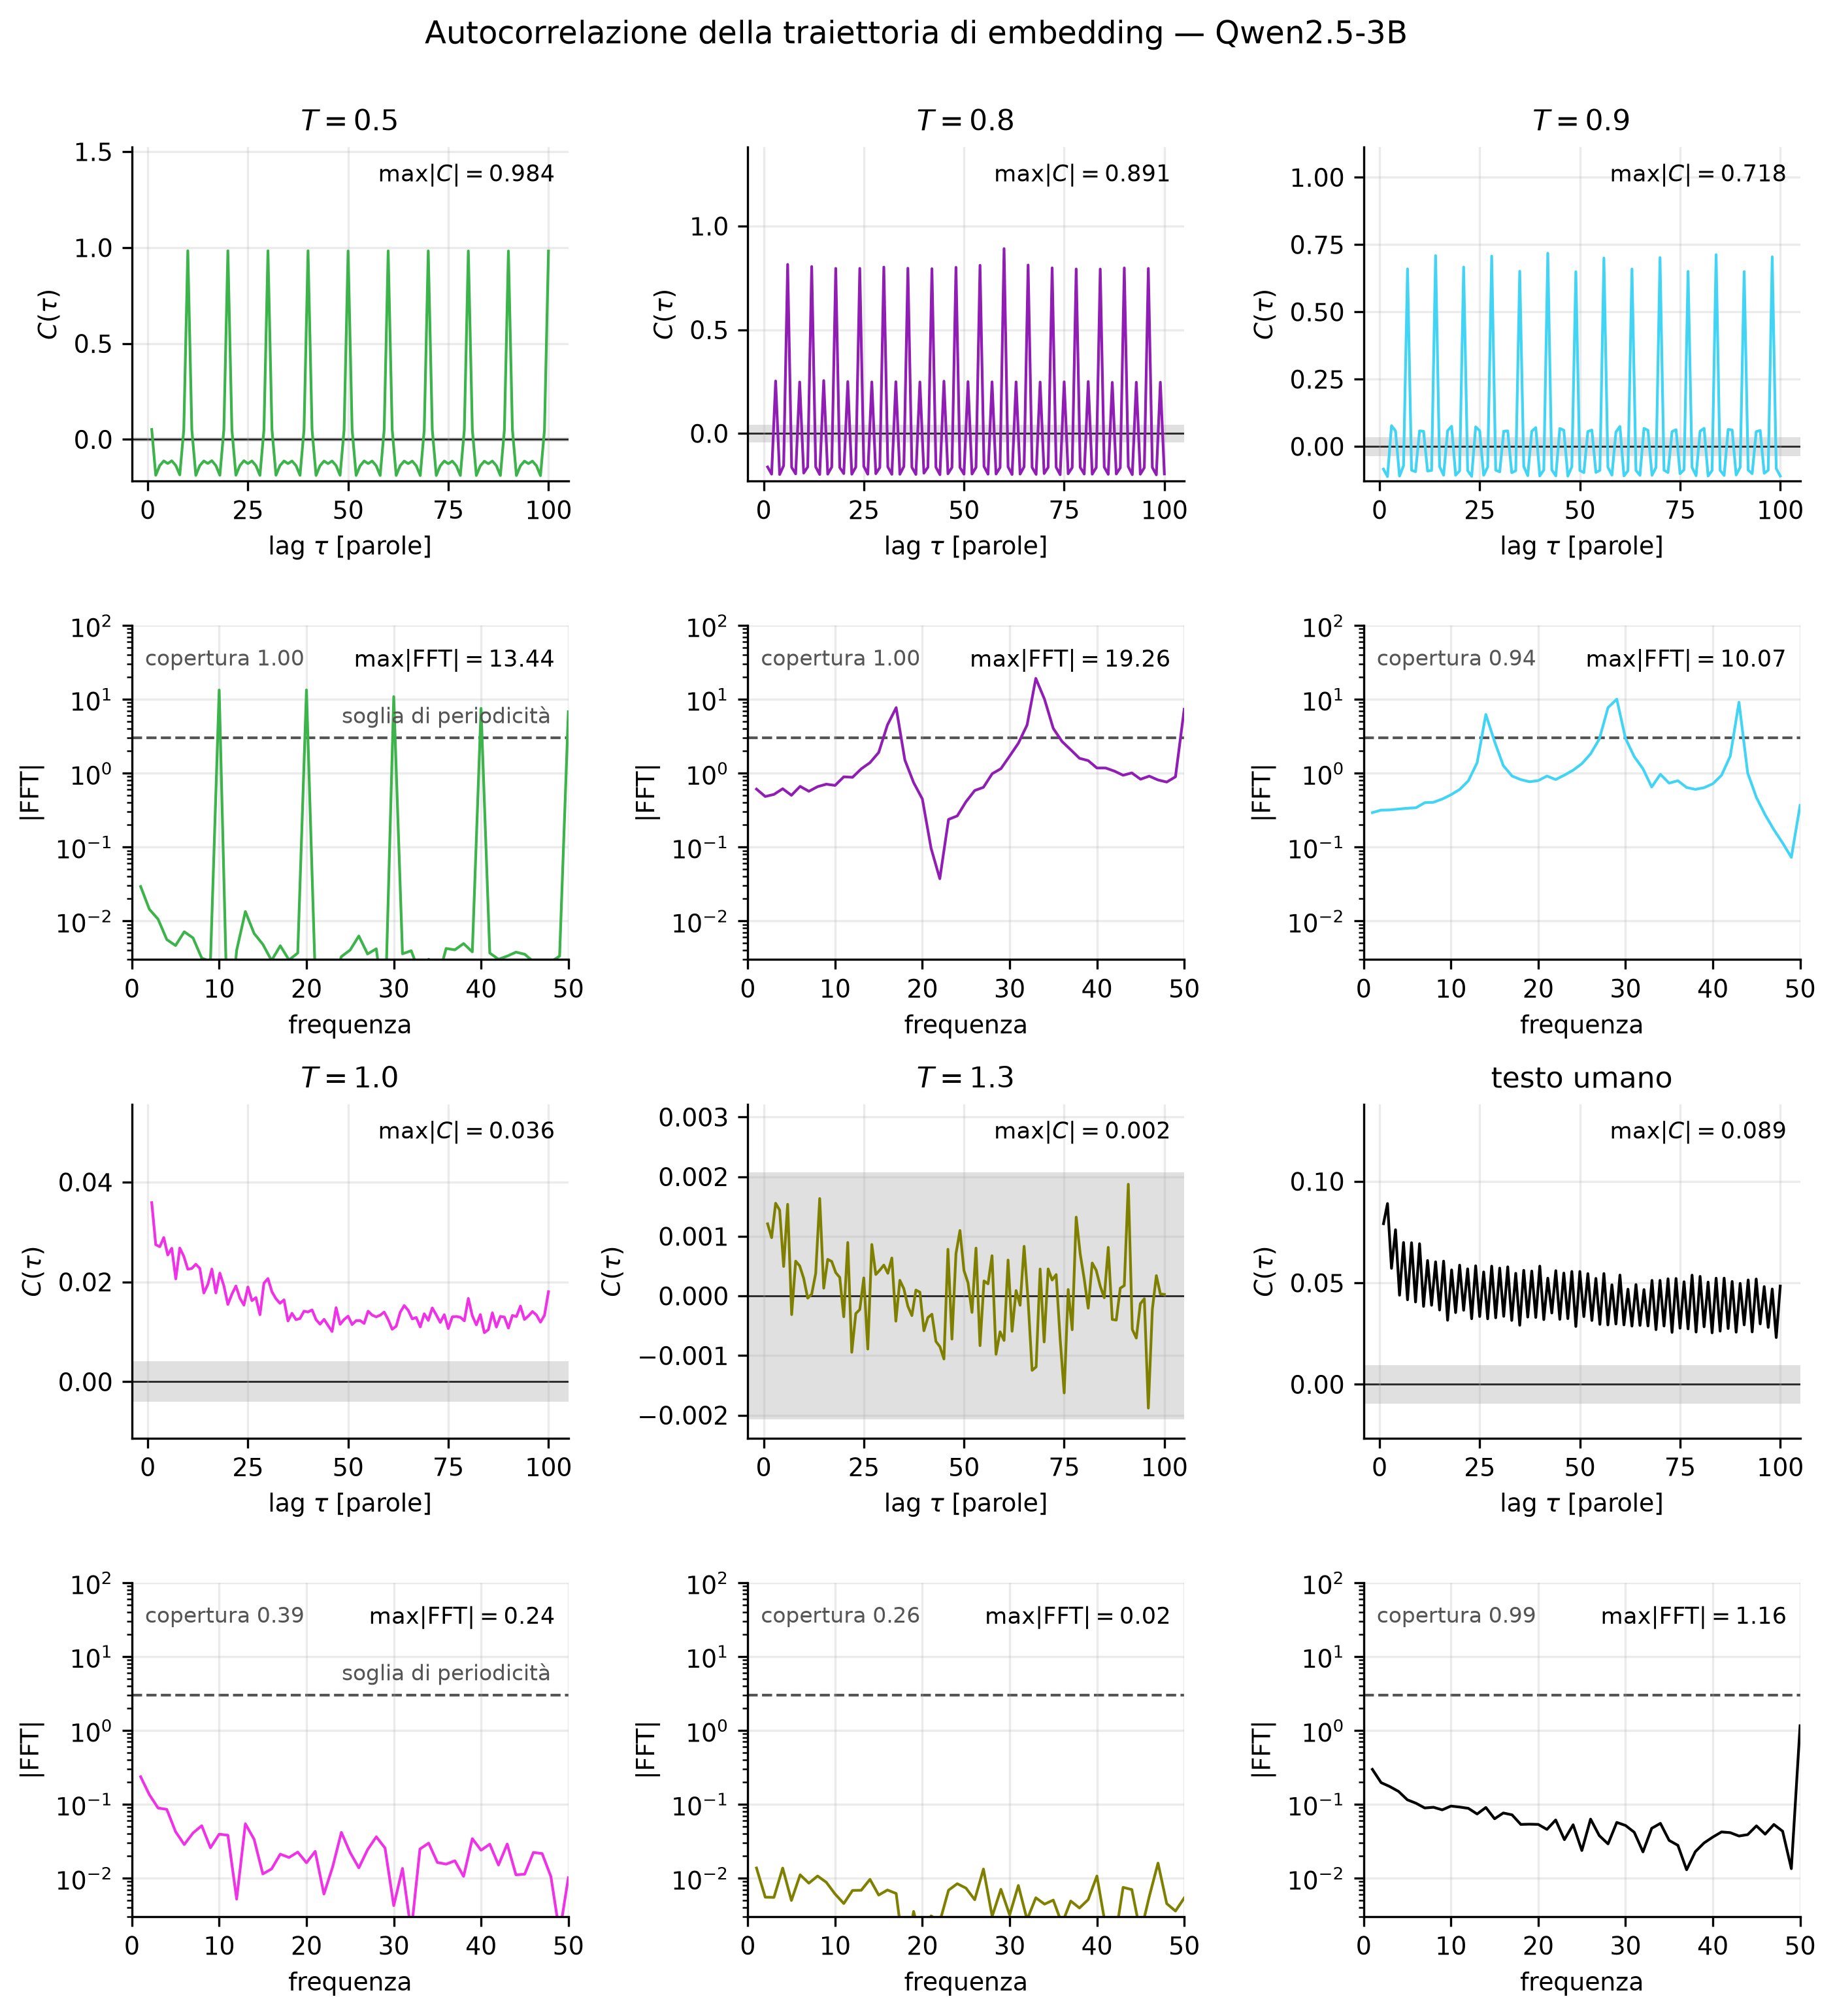
\includegraphics[width=\textwidth]{figure/cap4_acf_Qwen25_3B.png}
  \caption{Autocorrelazione della traiettoria di embedding per il modello
  Qwen2.5-3B a cinque temperature e sul testo umano di riferimento. In ciascuna
  coppia di riquadri il primo riporta $C(\tau)$ per lag da 1 a 100 parole e il
  secondo il modulo della sua trasformata di Fourier. La banda grigia è il
  livello di rumore, stimato ricalcolando $C(\tau)$ dopo aver permutato a caso
  le parole dello stesso documento; la linea tratteggiata è la soglia
  $\max\lvert\mathrm{FFT}\rvert = 3$ che separa la fase periodica. Per ogni
  temperatura è mostrato il campione di periodicità mediana, non il più marcato.
  La scala verticale di $C(\tau)$ è propria di ciascun riquadro, perché
  l'ampiezza varia di oltre due ordini di grandezza fra le temperature basse e
  quelle alte; il valore di picco è riportato dentro il riquadro. La scala dello
  spettro è invece logaritmica e comune, così i sei casi si confrontano
  direttamente.}
  \label{fig:acf}
\end{figure}

Il parametro d'ordine della prima transizione è il massimo modulo della
trasformata oltre il primo coefficiente, e il suo crollo è il risultato più
netto dell'intero capitolo. La media su tutti i modelli vale $16.0$ a
$T = 0.8$, scende a $7.5$ a $T = 0.9$ e precipita a $0.145$ a $T = 1.0$: un
fattore cinquanta in un solo passo di temperatura, e cento rispetto al massimo
di $T = 0.8$. Prosegue poi fino a $0.018$ a
$T = 1.5$, complessivamente tre ordini di grandezza sotto il massimo. Le cinque
curve dei diversi modelli si sovrappongono quasi esattamente, come mostra la
Figura~\ref{fig:transizioni}.

Anche questa soglia va confrontata con la fonte.
In~\cite{mikhaylovskiy2025states} la transizione dalla fase periodica è
collocata attorno a $t = 0.8$, con il testo dichiarato già non periodico a
$t = 1$, mentre qui la periodicità sopravvive fino a $T = 0.9$ e scompare a
$T = 1.0$. Lo spostamento verso l'alto è coerente con l'effetto del prompt
descritto nel §\ref{sec:protocollo}, che ritarda la comparsa delle proprietà
del regime disordinato.

\paragraph{Il secondo criterio non discrimina.} La distinzione fra stato
critico e fase amorfa dovrebbe essere operata dal GAPELMAPER, ma sui dati di
questo lavoro tale criterio non funziona. Il suo valore medio è $1.101$ con
deviazione standard $0.677$, e la quota di documenti con valore inferiore a 1,
cioè classificati come critici, è $0.51$: una moneta. Le barre d'errore nel
pannello centrale della Figura~\ref{fig:transizioni} sono di ampiezza
confrontabile con l'intero intervallo di variazione.

La difficoltà non è propria di questi dati. Lo stesso
\cite{mikhaylovskiy2025states} riporta che sui testi Qwen il GAPELMAPER è
raramente inferiore a 1, e che a diverse temperature del suo sweep non è
calcolabile affatto perché l'autocorrelazione assume valori negativi. Il
criterio, insomma, discrimina male anche nel lavoro che lo introduce.

Il motivo emerge dal terzo pannello. La copertura degli embedding resta sopra il
$95\%$ fino a $T = 0.9$, ma crolla a $0.64$ a $T = 1.0$ e a circa $0.31$ oltre
$T = 1.2$: nel regime in cui il GAPELMAPER dovrebbe distinguere le ultime due
fasi, l'autocorrelazione è calcolata su una minoranza delle parole e non
contiene più segnale. Per questa ragione i documenti che non superano la soglia
di copertura sono marcati come non valutabili anziché classificati, come
anticipato nel §\ref{sec:tre-fasi}. Senza tale precauzione il criterio avrebbe
assegnato una fase a documenti in cui non c'è nulla da misurare.

\paragraph{Il diagramma di fase.}
La Figura~\ref{fig:diagramma} riporta la composizione delle fasi per modello e
temperatura. Il quadro è coerente su tutti e cinque: fase periodica fino a
$T = 0.9$, dove la classificazione è ancora periodica per 13 documenti su 18;
scomparsa completa della periodicità a $T = 1.0$; documenti prevalentemente non
valutabili da $T = 1.1$ in poi, e completamente tali a $T \ge 1.4$.

\begin{figure}[htbp]
  \centering
  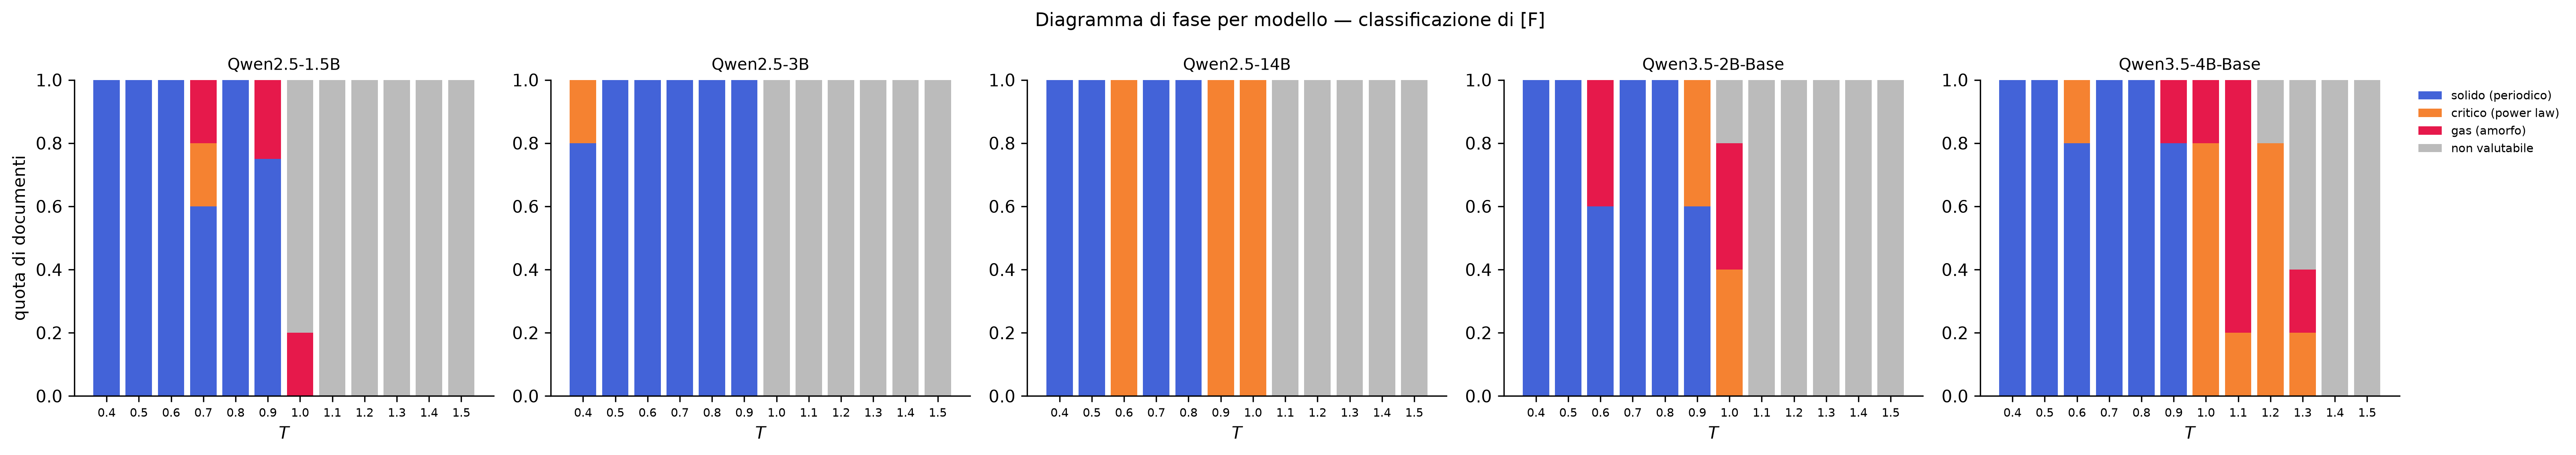
\includegraphics[width=\textwidth]{figure/cap4_diagramma_fase.png}
  \caption{Composizione delle fasi per modello e temperatura. La categoria «non
  valutabile» raccoglie i documenti che non superano la soglia di copertura
  degli embedding.}
  \label{fig:diagramma}
\end{figure}

Le tre modalità di fallimento del §\ref{sec:fallimenti} trovano qui la loro
interpretazione. La degenerazione per ripetizione è la fase periodica; la
degenerazione dell'alfabeto e del lessico corrisponde alla regione in cui la
misura non è più applicabile, che è a sua volta il segnale della fase amorfa. Il
testo non degenerato esiste solo nella striscia sottile fra le due, ed è la
stessa striscia in cui tutte le misure delle sezioni precedenti si avvicinano ai
valori umani.

% ---------------------------------------------------------------------
\section{Convergenza della temperatura critica}
\label{sec:tstar}

Le sezioni precedenti individuano ciascuna una temperatura privilegiata. Poiché
i criteri provengono da lavori indipendenti e misurano proprietà diverse del
testo, il loro accordo o disaccordo è esso stesso un risultato.

La Tabella~\ref{tab:tstar} riporta la temperatura selezionata da ciascun
criterio per ciascun modello. Due criteri sono intrinseci, nel senso che
individuano un estremo della curva senza far riferimento al testo umano: il
minimo del MAPE e la fine della fase periodica. Gli altri sei selezionano la
temperatura alla quale la misura si avvicina di più alla baseline umana.

\begin{table}[htbp]
\centering
\small
\begin{tabular}{@{}lccccc@{}}
\toprule
Criterio & 1.5B & 3B & 14B & 3.5-2B & 3.5-4B \\
\midrule
MAPE minimo                                  & 0.9 & 0.9 & 0.7 & 0.9 & 0.9 \\
$D_s$ minima dal testo umano                 & 0.9 & 0.9 & 0.9 & 0.9 & 1.0 \\
Fine della fase periodica                    & 1.0 & 1.0 & 0.6 & 1.0 & 1.0 \\
$R_{\mathrm{gzip}}$ più vicino all'umano     & 0.9 & 1.0 & 0.9 & 1.0 & 1.0 \\
$\alpha$ più vicino all'umano                & 1.0 & 1.5 & 1.3 & 1.0 & 1.0 \\
$R$ più vicino all'umano                     & 1.0 & 1.1 & 1.1 & 1.1 & 1.0 \\
$\gamma_H$ più vicino all'umano              & 1.1 & 1.0 & 1.3 & 1.1 & 1.3 \\
$\alpha_{\mathrm{DFA}}$ più vicino all'umano & 1.2 & 1.1 & 1.1 & 1.1 & 1.1 \\
\midrule
\textbf{mediana}                             & \textbf{1.0} & \textbf{1.0} &
\textbf{1.0} & \textbf{1.0} & \textbf{1.0} \\
\bottomrule
\end{tabular}
\caption{Temperatura selezionata da ciascun criterio, per ciascun modello. La
mediana vale $1.0$ per tutti e cinque i modelli, benché i singoli criteri
spazino da $0.6$ a $1.5$.}
\label{tab:tstar}
\end{table}

Il risultato principale del capitolo è la riga in fondo alla tabella. Otto
criteri tratti da quattro lavori indipendenti, costruiti per scopi diversi e mai
progettati per concordare, danno una mediana identica per tutti e cinque i
modelli. La convergenza non era scontata: i criteri misurano la distribuzione
delle frequenze, la crescita del vocabolario, le correlazioni a lungo raggio, la
comprimibilità e la periodicità dell'autocorrelazione, cioè proprietà che nulla
obbliga a coincidere.

\begin{figure}[htbp]
  \centering
  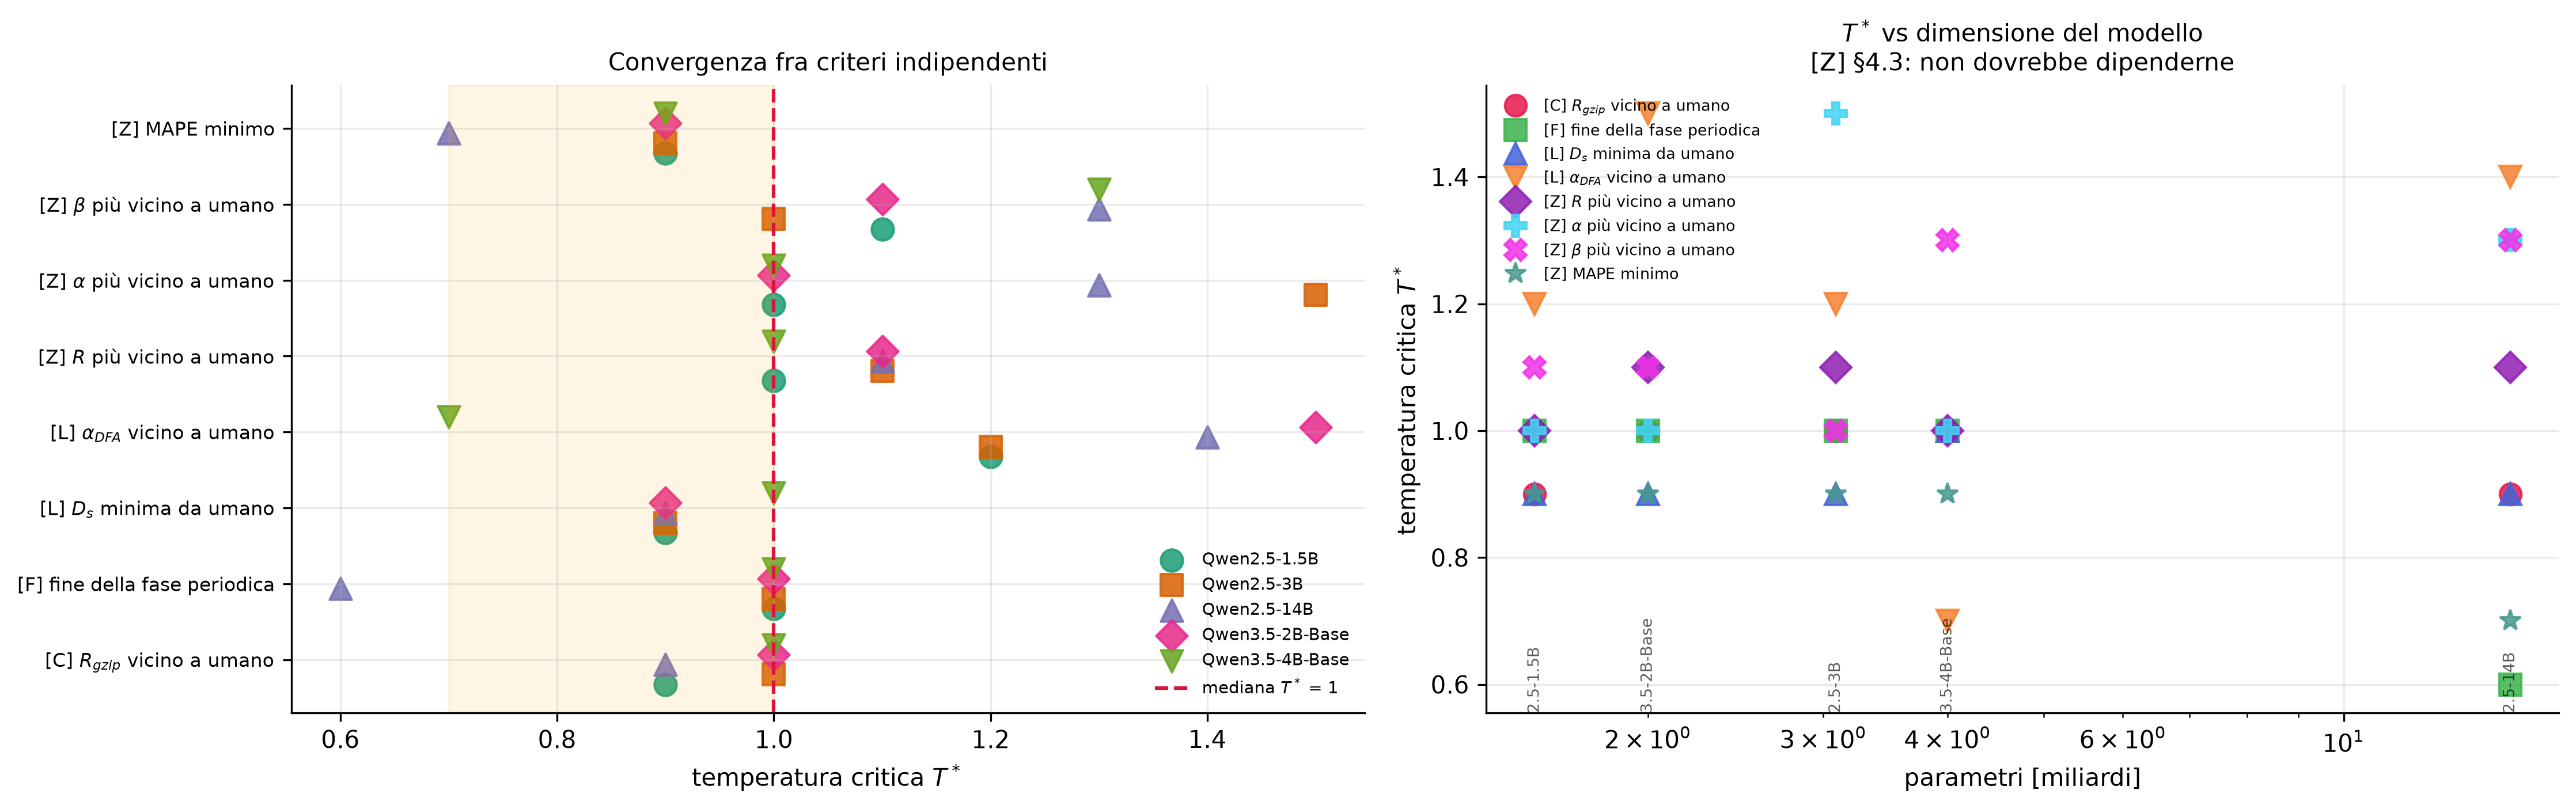
\includegraphics[width=\textwidth]{figure/cap4_temperatura_critica.png}
  \caption{A sinistra, la temperatura selezionata da ciascun criterio; la linea
  tratteggiata è la mediana complessiva e la banda la regione fra $0.7$ e $1.0$.
  A destra, la stessa quantità in funzione del numero di parametri del modello.}
  \label{fig:tstar}
\end{figure}

\paragraph{Dipendenza dalla dimensione del modello.}
La Figura~\ref{fig:tstar} riporta a destra la temperatura critica in funzione
del numero di parametri. La correlazione di rango è $\rho = -0.01$ con
$p = 0.93$ su quaranta osservazioni: nessuna dipendenza rilevabile. Il dato è
coerente con quanto riportato in~\cite{mikhaylovskiy2025zipf}, dove la posizione
dell'ottimo risulta indipendente dalla dimensione per tutte le famiglie
esaminate.

Un'assenza di correlazione misurata su cinque modelli appartenenti a due
famiglie non dimostra l'indipendenza: dimostra che, entro l'intervallo di
dimensioni esplorato e con la potenza statistica disponibile, non emerge
alcuna dipendenza. È coerenza con la letteratura, non conferma indipendente.

\paragraph{Una discordanza fra criteri.}
Due criteri si collocano sistematicamente fuori dal gruppo, e la loro distanza
dagli altri è essa stessa un risultato: mediarli insieme al resto la
cancellerebbe.

Il minimo del MAPE cade a $0.9$, mentre la fine della fase periodica cade a
$1.0$: alla temperatura in cui la distribuzione delle frequenze è più vicina a
una legge di potenza, l'autocorrelazione è ancora periodica per la maggioranza
dei documenti. Le due misure non si contraddicono, perché guardano oggetti
diversi, la statistica dei conteggi l'una e la struttura sequenziale l'altra,
e la loro distanza quantifica il fatto che le due proprietà non compaiono
simultaneamente. Il testo acquista una distribuzione di frequenze verosimile
prima di perdere la ripetizione.

Il criterio basato su $\alpha_{\mathrm{DFA}}$ merita una nota, perché il suo
esito dipende dall'ordine del detrending. Con il grado 1 seleziona temperature
fra $0.7$ e $1.5$, il più disperso dei nove; con il grado 2, che è quello
adottato qui per la ragione data nel §\ref{sec:robustezza}, si allinea agli
altri e sceglie $1.1$ per quattro modelli su cinque. La mediana per modello vale
$1.0$ in entrambi i casi. Resta valida l'avvertenza del
§\ref{sec:dfa-risultati}: alle basse temperature quell'esponente è instabile
fra documenti, e viene riportato per completezza anziché usato come criterio a
sé stante.

Una divergenza analoga fra criteri è documentata
in~\cite{mikhaylovskiy2025zipf} per i modelli Llama di grandi dimensioni, dove
le leggi di Zipf e di Heaps individuano temperature critiche sensibilmente
diverse. Il fenomeno non sembra dunque un artefatto di questo lavoro.

% ---------------------------------------------------------------------
\section{Che cosa lo sweep ha stabilito}
\label{sec:sintesi-cap4}

Tre risultati emergono dalle sezioni precedenti, di natura diversa fra loro.

Il primo è l'esistenza di una temperatura privilegiata, e la sua posizione. Otto
criteri costruiti per scopi diversi e tratti da quattro lavori indipendenti
danno una mediana identica, $T = 1.0$, per tutti e cinque i modelli, senza
dipendenza rilevabile dalla dimensione. Il secondo è che l'ottimo è stretto: la
transizione si consuma quasi interamente fra $T = 0.9$ e $T = 1.0$, dove il
parametro di periodicità cade di un fattore cinquanta, l'entropia passa da
$0.332$ a $5.77$ bit per carattere e il rapporto di compressione da $0.107$ a
$0.650$. Uno sweep a passo $0.1$ è appena sufficiente a risolvere quella
finestra.

Il terzo è l'esito negativo su cui poggia il capitolo successivo. L'esistenza
dell'ottimo è un fatto generale, ma la sua \emph{qualità} non lo è: due modelli
su cinque portano il MAPE al livello del testo umano e gli altri no. La
compressione condizionata non raggiunge il valore umano a nessuna temperatura,
ma per una ragione che non riguarda la struttura semantica: sotto la transizione
il testo ripete un ciclo e la seconda metà è prevedibile per costruzione, sopra
non è più linguaggio e non è prevedibile da nulla. Soprattutto, i documenti che
superano tutte e tre le soglie di non
degenerazione sono due su \num{242}. Il corpus generato lungo lo sweep non
sostiene quindi un'analisi semantica, ed è la ragione per cui il
Capitolo~\ref{cap:risultati2} cambia dominio anziché proseguire su questo.

Il capitolo non stabilisce però tutto. La convergenza dei criteri dice dove il
testo generato somiglia di più a quello umano secondo misure che ignorano il
significato; non dice se in quel punto il testo sia organizzato attorno a un
contenuto. È la domanda posta nel §\ref{sec:intro-domanda}, e richiede gli
strumenti del §\ref{sec:burst}.
%  Figure del corpo: modello Qwen2.5-3B. Quelle degli altri quattro
%  modelli stanno nel repository indicato in Appendice A.
% =====================================================================

\chapter{Il testo generato lungo lo sweep di temperatura}
\label{cap:risultati1}

Questo capitolo applica ai \num{242} documenti generati le misure introdotte nel
Capitolo~\ref{cap:teoria}, facendo variare la sola temperatura di campionamento.
Ogni misura viene confrontata con la baseline umana della
Tabella~\ref{tab:baseline}, calcolata con le stesse procedure e alla stessa
lunghezza.

Le figure del corpo del capitolo mostrano il modello Qwen2.5-3B, scelto come
esemplare perché dispone di cinque campioni per quasi tutte le temperature e
presenta le curve meno rumorose; le corrispondenti figure per gli altri quattro
modelli sono depositate nel repository indicato
nell'Appendice~\ref{app:codice}. Le curve aggregate
riportano invece tutti e cinque i modelli.

Il risultato principale non è nessuna delle singole misure, ma il fatto che
convergano: criteri tratti da quattro lavori indipendenti, costruiti per scopi
diversi, individuano la stessa regione di temperature. Il §\ref{sec:tstar} lo
documenta.

% ---------------------------------------------------------------------
\section{Le tre modalità di fallimento}
\label{sec:fallimenti}

La prima e la terza riga della Tabella~\ref{tab:tre-regimi} sono entrambe
prodotte dai modelli qui analizzati, a due temperature diverse, e mostrano i
due modi in cui la generazione si allontana dal linguaggio: la ripetizione letterale a bassa
temperatura, l'incoerenza semantica ad alta temperatura. Salendo ancora si
incontra un terzo regime, in cui l'alfabeto stesso si disgrega e il testo diventa
un miscuglio di sistemi di scrittura diversi.

Le tre modalità possono essere separate quantitativamente. Un documento viene
classificato come degenerato per \emph{ripetizione} se la quota di 8-grammi
ripetuti supera $0.10$, contro il valore $0.000$ misurato sul testo umano; come
degenerato nell'\emph{alfabeto} se la quota di caratteri non ASCII supera
$0.05$, più del triplo del valore umano $0.014$; come degenerato nel
\emph{lessico} se meno del $70\%$ delle sue parole possiede un vettore nello
spazio di embedding, contro il $98\%$ del testo umano. Le tre condizioni non si
escludono a vicenda, e un documento può soddisfarne più di una.

La Tabella~\ref{tab:fallimenti} riporta i conteggi.

\begin{table}[htbp]
\centering
\small
\begin{tabular}{@{}l>{\raggedright\arraybackslash}p{5.4cm}rr@{}}
\toprule
Modalità & Criterio & Documenti & Quota \\
\midrule
Ripetizione & 8-grammi ripetuti $> 0.10$      & 122 & 50\,\% \\
Alfabeto    & caratteri non ASCII $> 0.05$    & 125 & 52\,\% \\
Lessico     & copertura degli embedding $< 0.70$ & 112 & 46\,\% \\
\midrule
Nessuna     & prosa inglese non degenerata    &   2 &  1\,\% \\
\bottomrule
\end{tabular}
\caption{Modalità di degenerazione dei \num{242} documenti generati. Le
categorie non sono disgiunte. La classificazione dipende dalle soglie scelte,
ma non nella sostanza: facendole variare entro intervalli ragionevoli il numero
di documenti non degenerati resta compreso fra 2 e 7, cioè fra l'uno e il tre
per cento del totale.}
\label{tab:fallimenti}
\end{table}

Il dato va letto con attenzione, perché è il presupposto dell'intera seconda
parte sperimentale. Non significa che i modelli siano incapaci di produrre
linguaggio, ma che la finestra di temperature in cui lo producono è
sufficientemente stretta da non essere coperta da uno sweep a passo $0.1$: i
soli due documenti non degenerati compaiono a $T = 1.0$, e già a $T = 0.9$ e
$T = 1.1$ tutti i campioni ricadono in almeno una delle tre categorie. Il
Capitolo~\ref{cap:risultati2} muove da questa constatazione.


% ---------------------------------------------------------------------
\section{Legge di Zipf}
\label{sec:zipf-risultati}

La Figura~\ref{fig:zipf-cum} riporta gli istogrammi cumulativi delle frequenze,
una curva per temperatura, con la curva umana per confronto.

\begin{figure}[htbp]
  \centering
  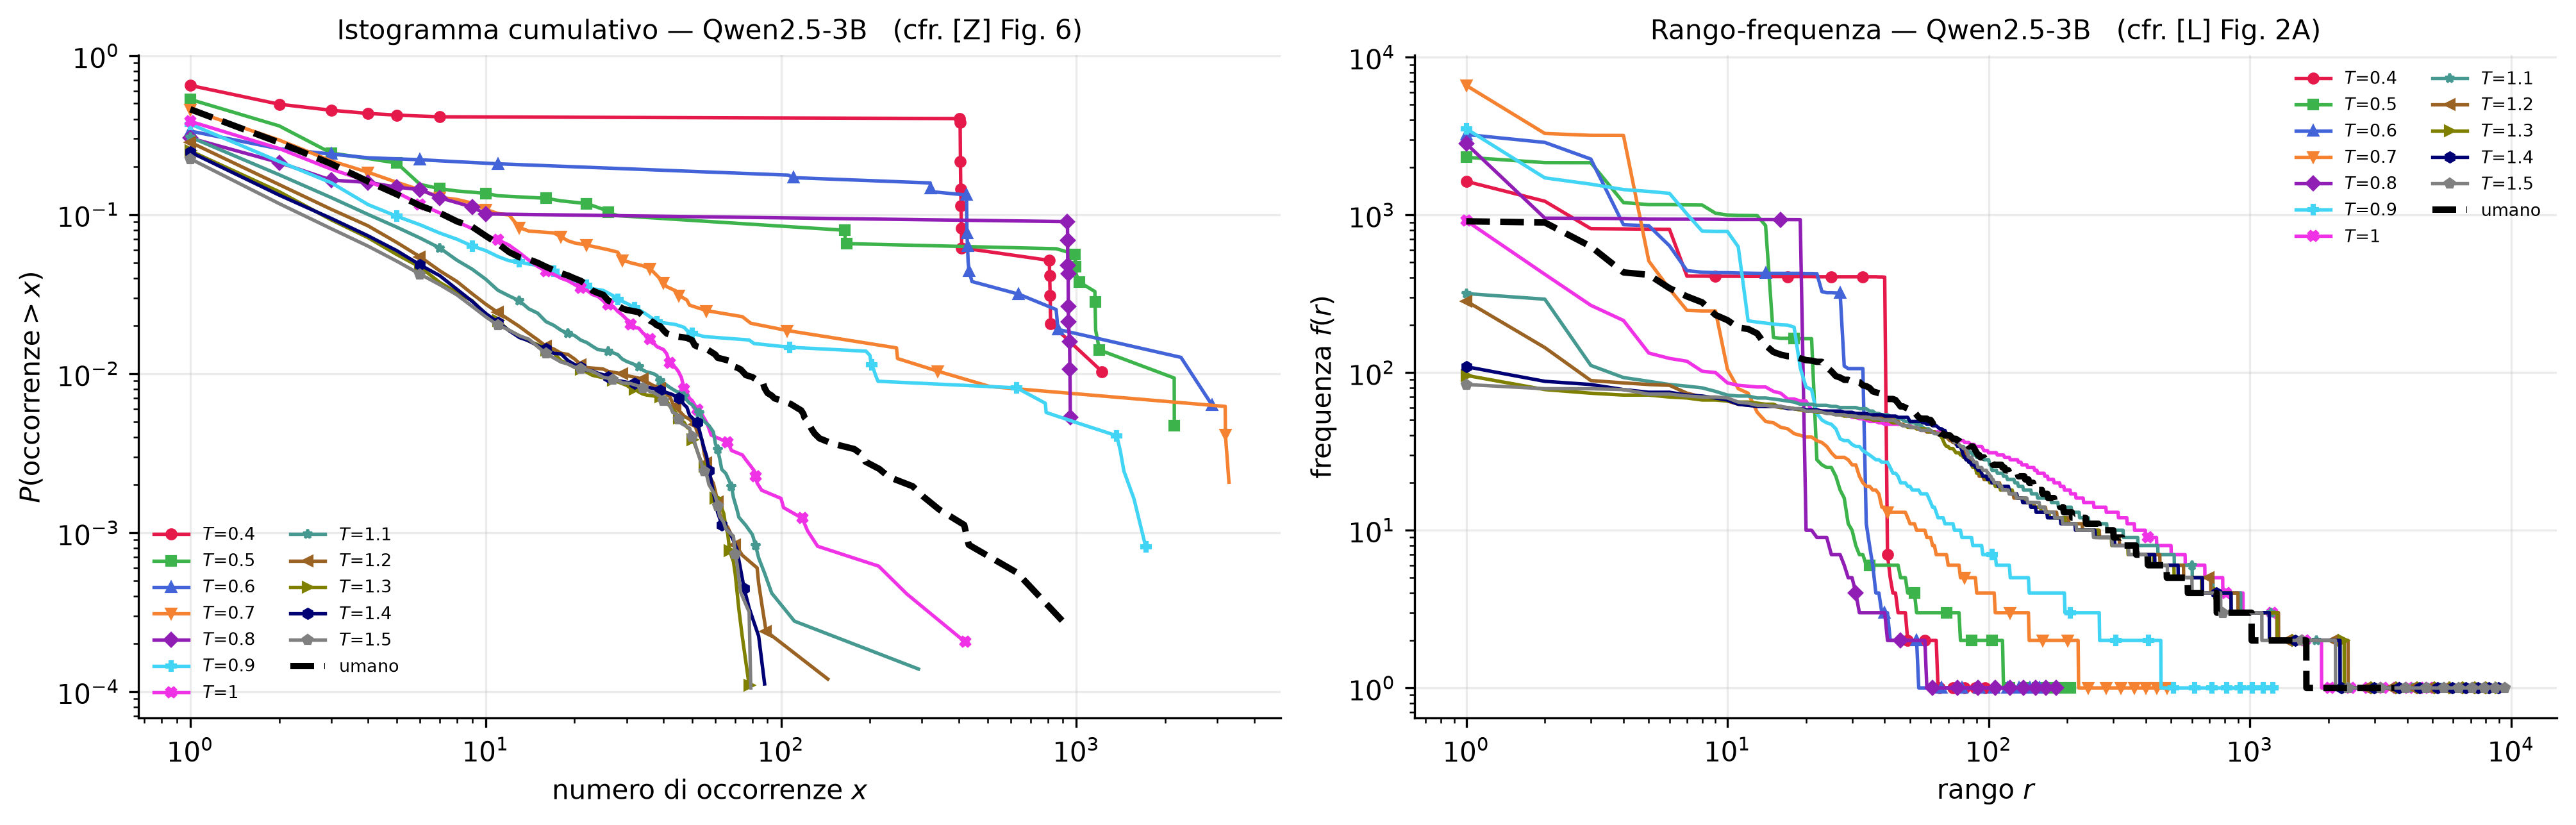
\includegraphics[width=\textwidth]{figure/cap4_zipf_cumulativo_Qwen25_3B.png}
  \caption{Istogrammi cumulativi delle frequenze dei token per il modello
  Qwen2.5-3B, una curva per temperatura. A bassa temperatura la curva è quasi
  verticale, perché pochi token coprono l'intero documento; ad alta temperatura
  è quasi orizzontale, perché quasi ogni token compare una volta sola. Solo
  nella regione intermedia la curva si avvicina alla retta che in coordinate
  bilogaritmiche corrisponde a una legge di potenza.}
  \label{fig:zipf-cum}
\end{figure}

L'esponente da solo non basta a descrivere questo comportamento, ed è la ragione
per cui nel §\ref{sec:zipf} è stato introdotto il MAPE: una curva può avere la
pendenza corretta e una curvatura marcata, e in tal caso l'esponente stimato non
descrive nulla. La Figura~\ref{fig:zipf-vs-T} riporta entrambe le quantità in
funzione della temperatura.

\begin{figure}[htbp]
  \centering
  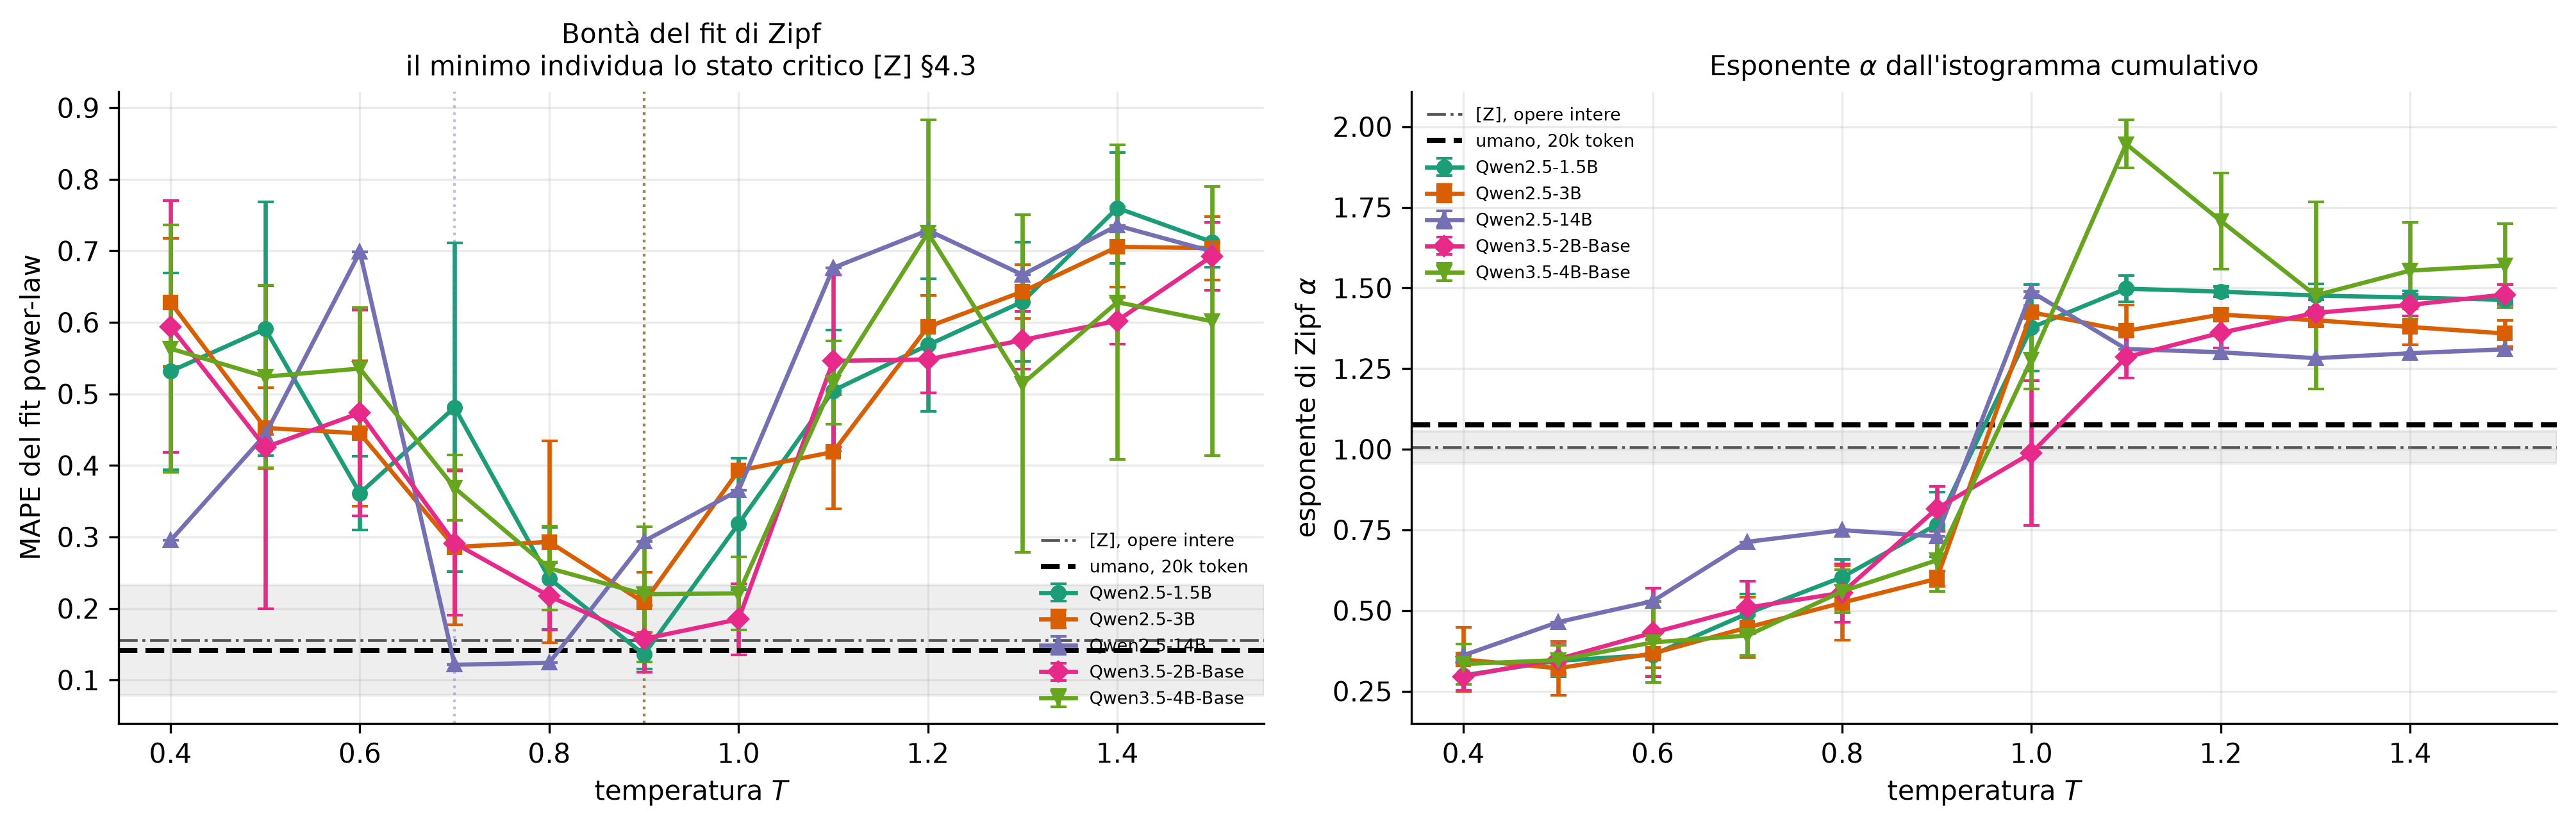
\includegraphics[width=\textwidth]{figure/cap4_zipf_vs_T.png}
  \caption{Bontà del fit e esponente della legge di Zipf in funzione della
  temperatura, per tutti e cinque i modelli. La banda grigia è il valore
  pubblicato su testi letterari interi, la linea nera tratteggiata la baseline
  umana misurata alla lunghezza di lavoro.}
  \label{fig:zipf-vs-T}
\end{figure}

Il MAPE ha un minimo pronunciato, che cade a $T = 0.9$ per quattro modelli su
cinque e a $T = 0.7$ per il modello da 14 miliardi di parametri. È il
risultato centrale della sezione: esiste una temperatura alla quale la
distribuzione delle frequenze del testo generato è più vicina a una legge di
potenza, e ai due lati di essa l'aderenza peggiora rapidamente.

Al minimo il MAPE del modello esemplare vale $0.208$. I due termini di
riferimento sono la baseline umana misurata alla stessa lunghezza, che vale
$0.141$, e il valore $0.156 \pm 0.077$ che~\cite{mikhaylovskiy2025zipf} riporta
su un corpus di sei opere letterarie in cinque lingue. Che i due riferimenti
umani cadano tanto vicini è una verifica indipendente della taratura della
baseline: sono ottenuti con tokenizzatori diversi, su testi diversi e di
lunghezza diversa, e la deriva documentata nella
Figura~\ref{fig:dimensione-finita} non rendeva scontato l'accordo.

Il valore del modello va letto contro tre metri diversi, e il giudizio che se ne
ricava non è lo stesso. Rispetto al modello stesso, $0.208$ è un risultato
netto: alle due estremità dell'intervallo lo stesso modello dà $0.628$ e
$0.704$, cioè un errore di fit tre volte più grande. Rispetto al testo umano è
invece una mezza vittoria: $0.208$ è circa una volta e mezza $0.141$, e resta
dentro la banda pubblicata solo perché quella banda è larga, sfiorandone il
margine superiore $0.233$. Rispetto agli altri modelli, infine, è un risultato
mediocre. La Tabella~\ref{tab:mape-minimi} riporta i cinque minimi: due modelli
scendono sotto il valore umano e un terzo vi si accosta, con $0.158$ contro
$0.141$, mentre il modello esemplare e il Qwen3.5-4B restano sopra.

\begin{table}[htbp]
\centering
\small
\begin{tabular}{@{}lrr@{}}
\toprule
Modello & $T$ del minimo & MAPE al minimo \\
\midrule
Qwen2.5-14B      & 0.7 & 0.121 \\
Qwen2.5-1.5B     & 0.9 & 0.136 \\
Qwen3.5-2B-Base  & 0.9 & 0.158 \\
Qwen2.5-3B       & 0.9 & 0.208 \\
Qwen3.5-4B-Base  & 0.9 & 0.220 \\
\midrule
testo umano      & --- & 0.141 \\
\bottomrule
\end{tabular}
\caption{Valore minimo del MAPE e temperatura alla quale viene raggiunto, per
ciascun modello, con la baseline umana misurata alla stessa lunghezza. Il
minimo esiste per tutti e cinque, ma solo tre modelli lo portano al livello del
testo umano o sotto. La riga del Qwen2.5-14B è ricavata da un solo campione per
temperatura e va letta con la cautela discussa nel testo.}
\label{tab:mape-minimi}
\end{table}

La prima riga della tabella richiede una precauzione. Il Qwen2.5-14B è l'unico
modello con un solo campione per temperatura, contro i tre o cinque degli altri,
e la sua curva del MAPE non è regolare da nessuno dei due lati del minimo: vale
$0.295$ a $T = 0.4$, sale a $0.698$ a $T = 0.6$ e scende a $0.121$ a $T = 0.7$,
cioè peggiora di un fattore due e migliora di un fattore sei in due passi
consecutivi. Negli altri quattro modelli la dispersione fra campioni alla stessa
temperatura va da $0.046$ a $0.230$ attorno a $T = 0.7$, mentre la distanza fra
il minimo del 14B e il suo valore a $T = 0.9$ vale $0.173$: sta dentro
quell'intervallo. Con una sola realizzazione la posizione del minimo non è
risolvibile, e il valore $T = 0.7$ va letto come compatibile con il $T = 0.9$
degli altri quattro anziché come uno spostamento reale. La stessa cautela vale
per la profondità: $0.121$ è il minimo più basso dei cinque ed è anche il meno
affidabile, mentre il $0.136$ del Qwen2.5-1.5B poggia su cinque campioni con
dispersione $0.020$ ed è l'unico caso in cui il primato sul testo umano è
sostenuto da repliche.

La posizione del minimo va confrontata con quella riportata nella fonte.
In~\cite{mikhaylovskiy2025zipf} il minimo del MAPE cade fra $t = 1.0$ e
$t = 1.2$ per tutti i modelli tranne i Llama più grandi, mentre qui cade a
$T = 0.9$ per quattro modelli su cinque. Lo scarto è nella direzione prevista
dall'effetto del prompt descritto nel §\ref{sec:protocollo}, che abbassa
l'errore del fit soprattutto alle basse temperature e sposta quindi il minimo
verso sinistra.

Ne segue una distinzione che vale per tutto il seguito. L'esistenza
di una temperatura ottimale è un fatto generale, comune a tutti e cinque i
modelli; la qualità dell'ottimo, cioè quanto il testo generato in quel punto
somigli davvero a un testo umano, varia da modello a modello e non è garantita.
Il modello scelto come esemplare non è fra quelli che ci riescono, e i grafici
del corpo del capitolo vanno letti tenendolo presente.

L'esponente $\alpha$ racconta la stessa storia da un'altra angolazione. Per il
modello esemplare passa da $0.35$ a $T = 0.4$, valore che corrisponde a una
distribuzione dominata da pochissimi tipi, a $1.36$ a $T = 1.5$, dove più di tre
quarti dei tipi compaiono una volta sola.\footnote{Un tipo che compare una sola
volta nel testo si dice \emph{hapax}. Gli hapax sono normalmente la maggioranza
dei tipi ma una piccola parte delle occorrenze: nella baseline umana usata qui
sono il $54\%$ dei tipi e il $10\%$ dei token, mentre a $T = 1.5$ il modello
esemplare arriva al $77\%$ dei tipi e al $37\%$ dei token.} La transizione non è
graduale: fra $T = 0.9$ e $T = 1.0$ l'esponente salta da $0.60$ a $1.43$,
attraversando in un solo passo il valore umano $1.076$, per poi assestarsi
attorno a $1.4$ senza più avvicinarvisi.

% ---------------------------------------------------------------------
\section{Legge di Heaps e descrittore \texorpdfstring{$R$}{R}}
\label{sec:heaps-risultati}

Le curve di crescita del vocabolario rendono immediatamente evidente perché il
§\ref{sec:heaps} abbia dovuto introdurre un descrittore alternativo all'esponente di
Heaps.

\begin{figure}[htbp]
  \centering
  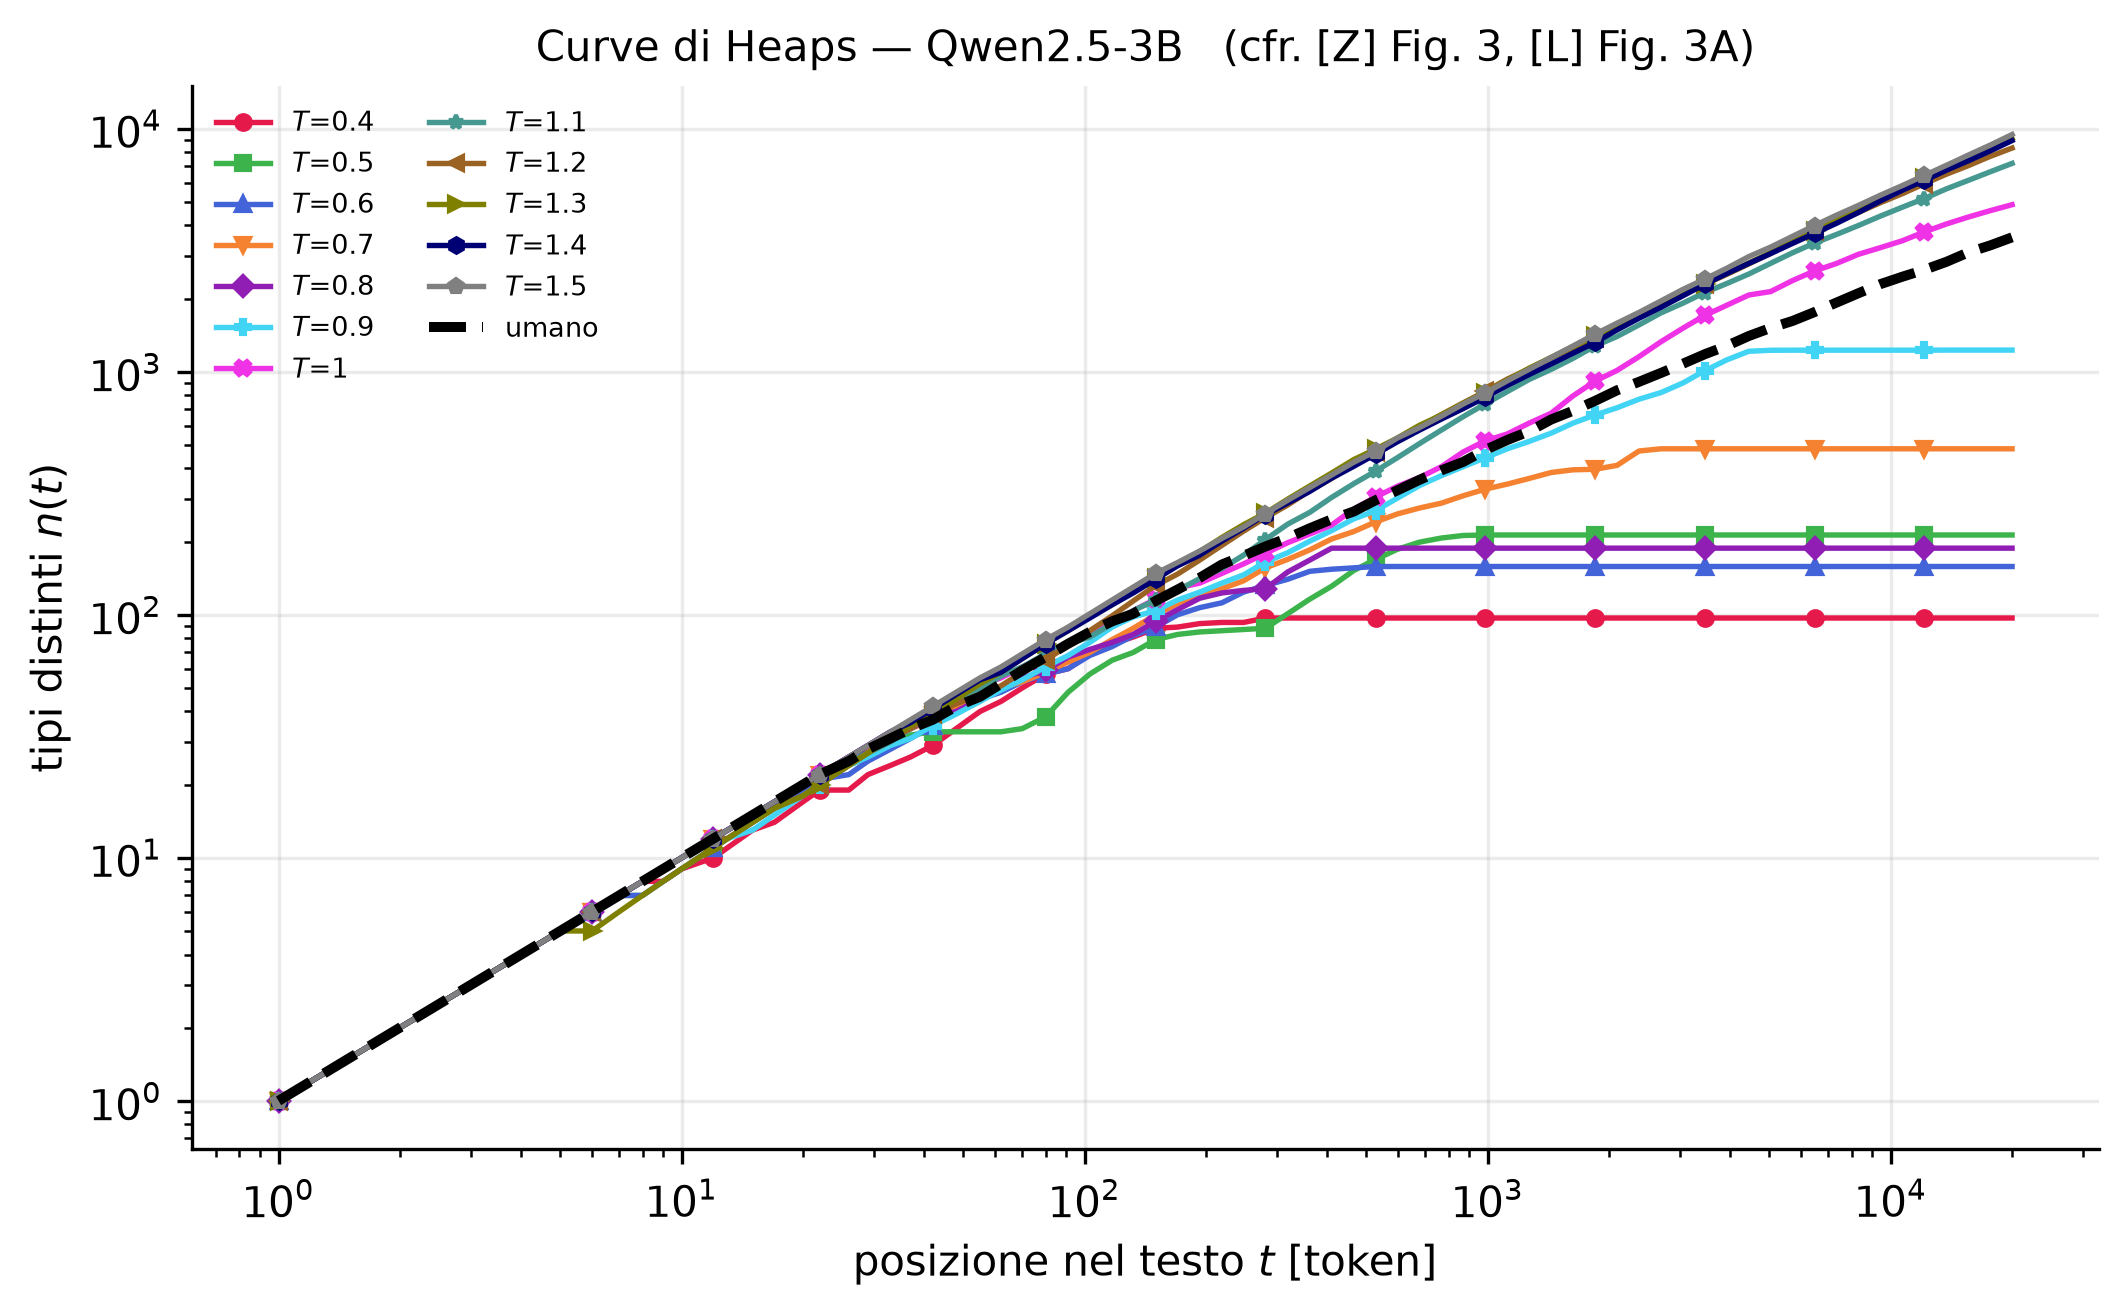
\includegraphics[width=0.86\textwidth]{figure/cap4_heaps_curve_Qwen25_3B.png}
  \caption{Crescita del vocabolario per il modello Qwen2.5-3B. Alle temperature
  basse la curva si appiattisce dopo poche migliaia di token: il modello ha
  smesso di produrre tipi nuovi. Alle temperature alte cresce quasi linearmente.
  In nessuno dei due casi la curva è una legge di potenza, e stimarne
  l'esponente restituisce un numero privo di contenuto.}
  \label{fig:heaps-curve}
\end{figure}

La Figura~\ref{fig:heaps-R} riporta il descrittore $R$, l'esponente $\gamma_H$
e il rapporto fra tipi e occorrenze in funzione della temperatura. I tre
andamenti sono concordi: per il modello esemplare $\gamma_H$ passa da $0.001$
a $T = 0.4$, dove la curva è piatta e il vocabolario non cresce affatto, a
$0.806$ a $T = 1.5$, attraversando il valore umano $0.668$ poco sopra $T =
0.9$. Il descrittore $R$ passa da $0.003$ a $0.688$ e incrocia il valore umano
$0.507$ attorno a $T = 1.05$.

Il terzo pannello riporta la quantità più elementare delle tre, il rapporto fra
il numero di tipi distinti e il numero di occorrenze, e serve da controllo sulle
altre due. A differenza di $\gamma_H$ e di $R$ non richiede alcun fit né alcuna
partizione del documento, quindi non può essere alterato da un modello mal
specificato: se le tre curve concordano, l'andamento non è un artefatto della
procedura di stima. Per il modello esemplare passa da $0.007$ a $T = 0.4$ a
$0.474$ a $T = 1.5$, e attraversa il valore umano $0.179$ fra $T = 0.9$ e
$T = 1.0$, cioè nello stesso punto delle altre due misure. Il pannello mostra
però anche in che senso l'accordo con il testo umano sia solo locale: sopra
$T = 1.1$ il rapporto supera il doppio del valore umano e continua a crescere,
mentre $\gamma_H$ resta stabile attorno a $0.8$. Le due misure smettono di dire
la stessa cosa non appena il vocabolario si allarga oltre quello di un romanzo.

\begin{figure}[htbp]
  \centering
  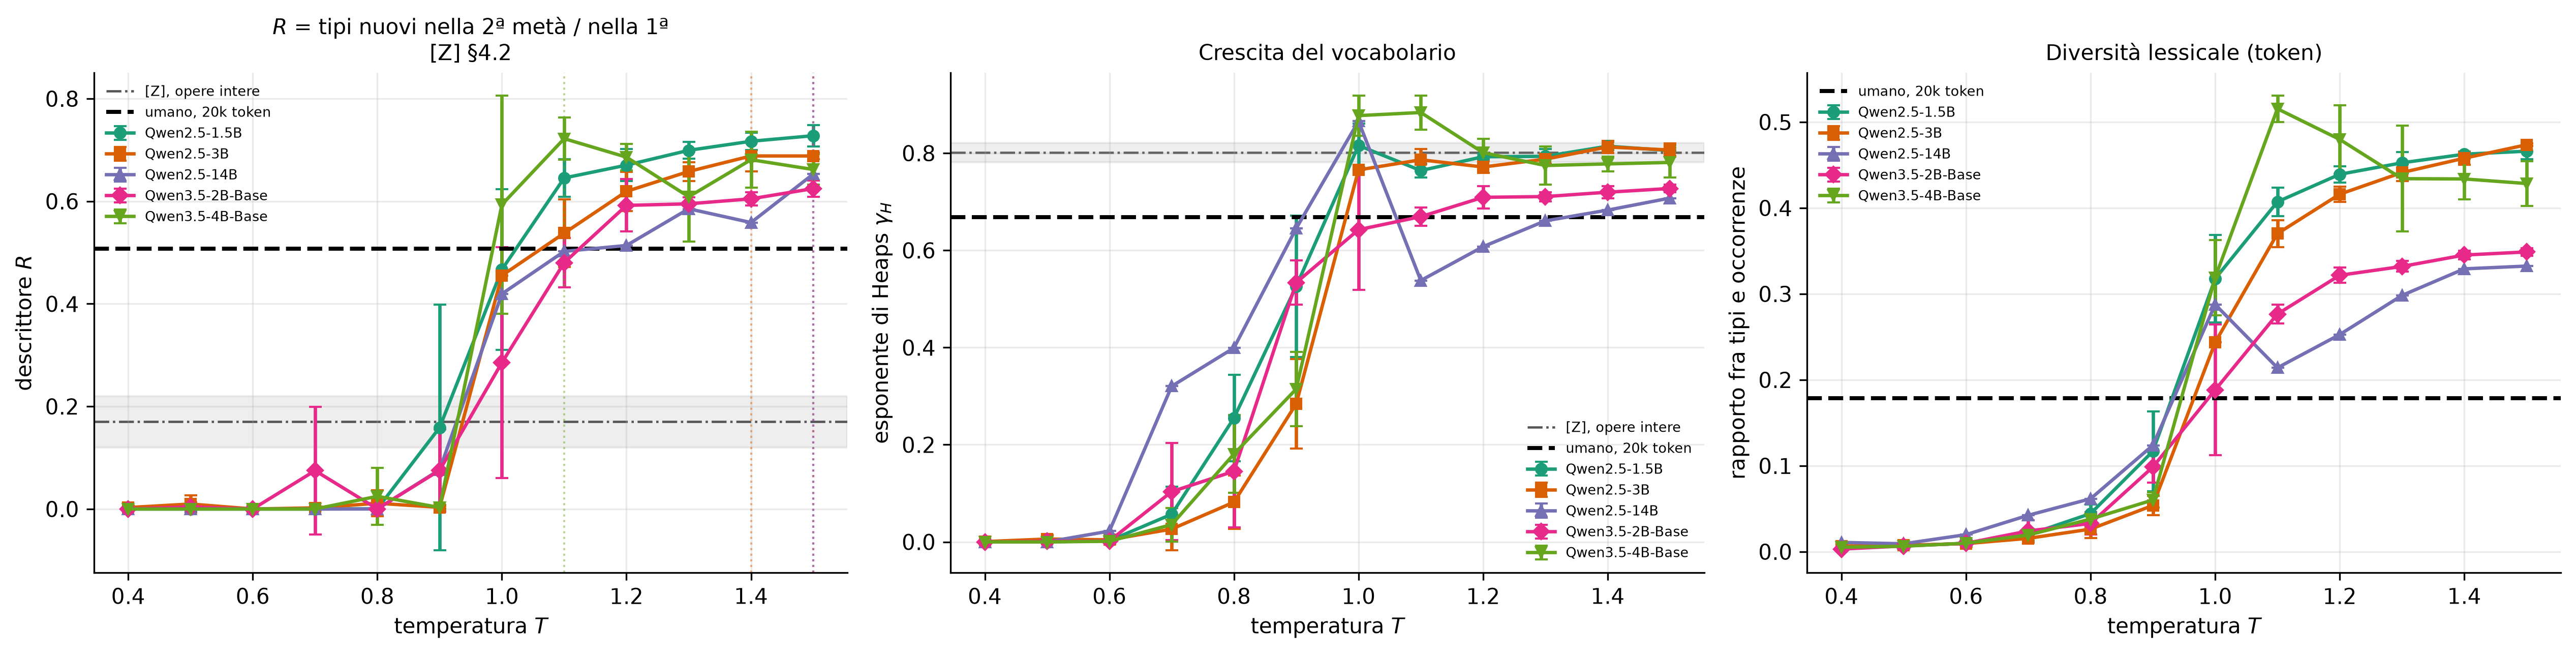
\includegraphics[width=\textwidth]{figure/cap4_heaps_R_vs_T.png}
  \caption{Descrittore $R$, esponente di Heaps e rapporto fra tipi e occorrenze
  in funzione della temperatura. La banda grigia riporta i valori pubblicati su
  opere intere, che per le ragioni discusse nel §\ref{sec:scelte} non sono un
  termine di confronto diretto.}
  \label{fig:heaps-R}
\end{figure}

% ---------------------------------------------------------------------
\section{Correlazioni a lungo raggio}
\label{sec:dfa-risultati}

Ogni documento viene convertito nella successione numerica definita nel
§\ref{sec:dfa}: ogni carattere è sostituito dal proprio rango di frequenza nel
documento, $1$ al più frequente, $2$ al secondo, e così via. È su quella
successione che si misura l'esponente della fluttuazione. Il detrending è
quadratico: il §\ref{sec:robustezza} documenta il confronto con quello lineare e
la ragione della scelta, cioè che alle basse temperature i documenti non sono
stazionari e un polinomio di primo grado non assorbe la deriva della
composizione dei caratteri. Il primo controllo riguarda il null model: la stessa
analisi condotta sui documenti rimescolati deve restituire un esponente pari a
$1/2$.


La Figura~\ref{fig:dfa} riporta le curve di fluttuazione e l'esponente in
funzione della temperatura. L'esponente ha un massimo a $T = 1.0$, dove vale
$0.719$ in media su tutti i modelli, superiore al valore umano di $0.579$;
decresce poi verso $0.53$ alle temperature più alte, avvicinandosi al valore del
rimescolamento senza raggiungerlo.

\begin{figure}[htbp]
  \centering
  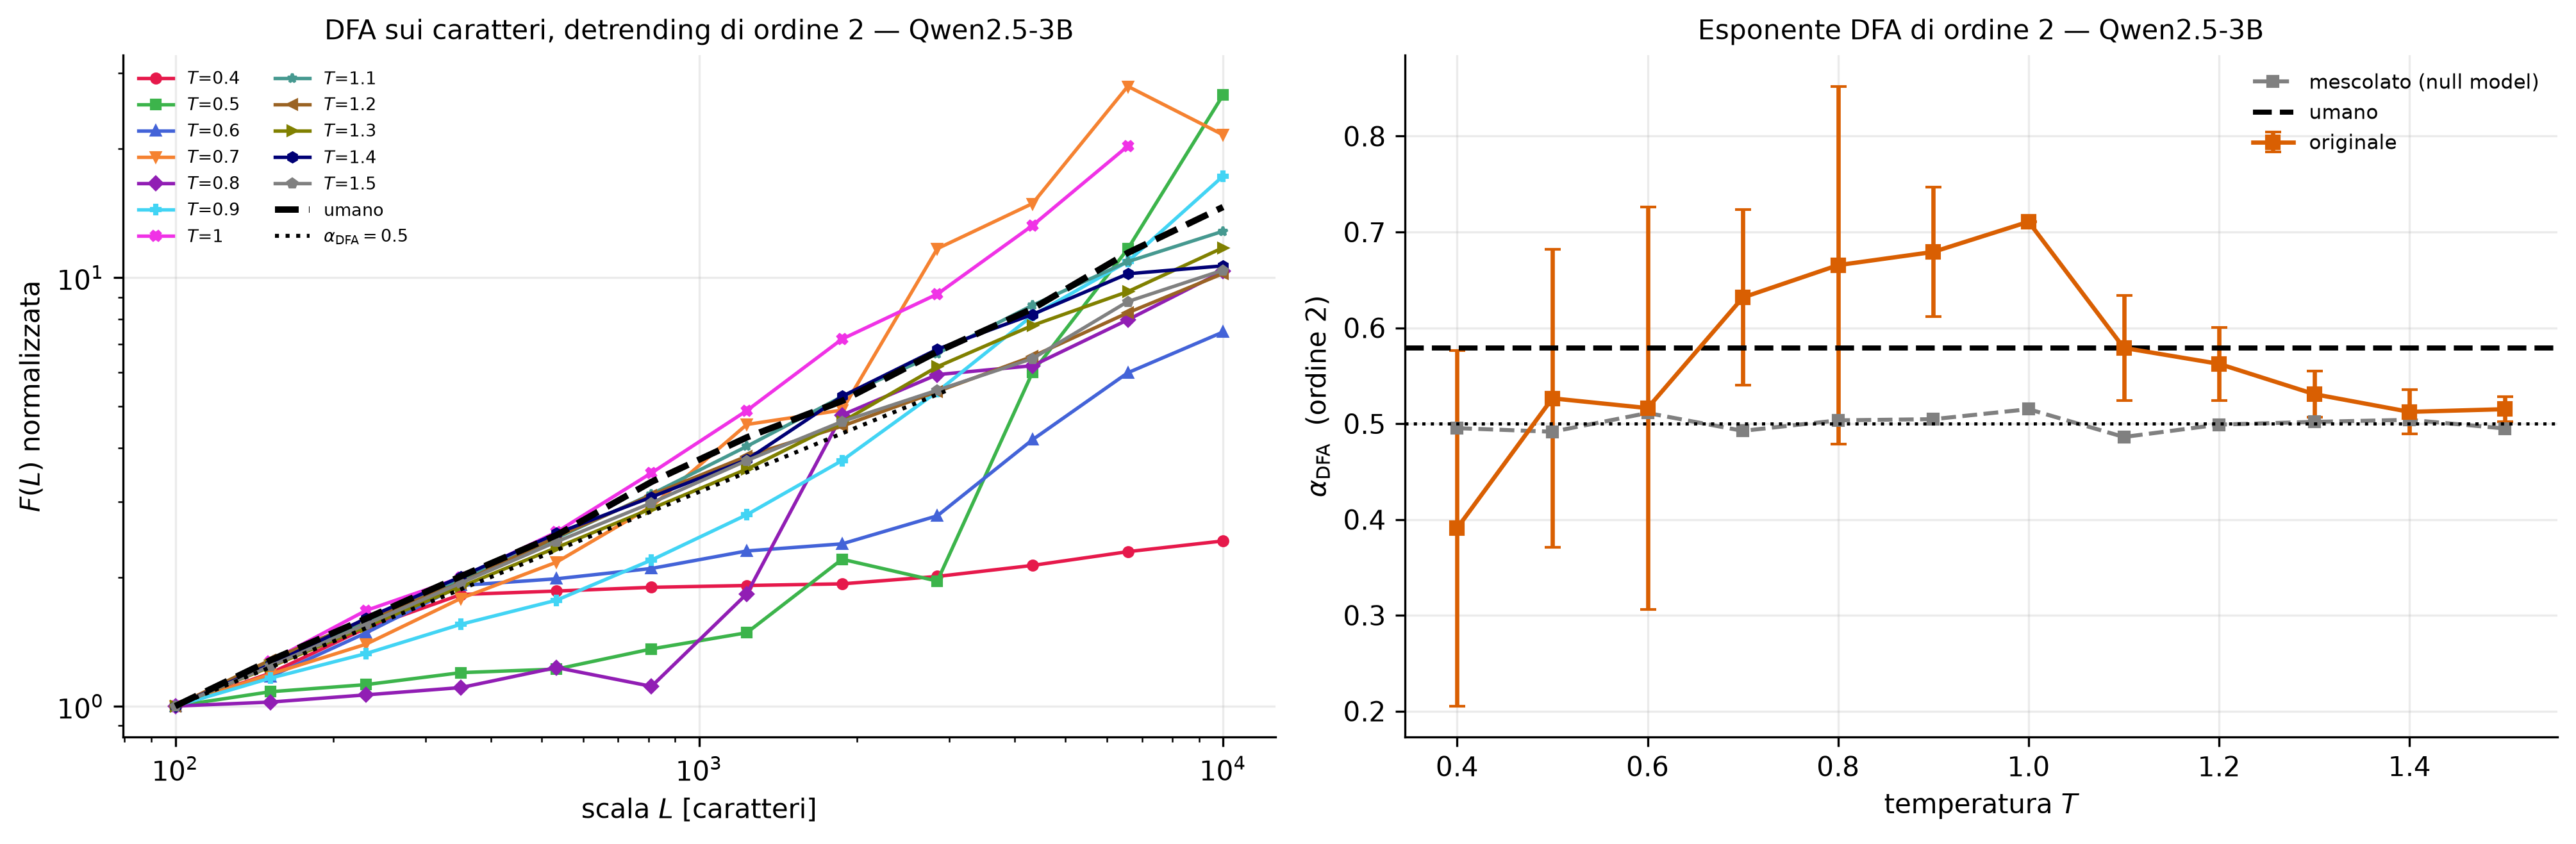
\includegraphics[width=\textwidth]{figure/cap4_dfa_Qwen25_3B_o2.png}
  \caption{Fluttuazione detrendizzata per il modello Qwen2.5-3B, con detrending
  quadratico. A sinistra $F(s)$ in funzione della scala, una curva per
  temperatura, con la pendenza di riferimento $\alpha_{\mathrm{DFA}} = 1/2$; a
  destra l'esponente in funzione della temperatura, con il null model
  rimescolato e la baseline umana.}
  \label{fig:dfa}
\end{figure}

\paragraph{La dispersione è il vero segnale.}
Il valore medio dell'esponente nasconde il fenomeno più informativo, ed è un
fenomeno già osservato: sulle reti LSTM~\cite{lippi2019} riporta che le stime
sui singoli campioni sono molto disperse attorno a $T = 0.5$ e strettamente
raccolte attorno alla media a $T = 1.0$. Gli stessi dati mostrano qui lo stesso
comportamento su architetture transformer. La deviazione standard fra documenti
passa da $0.219$ a $T = 0.4$ a $0.022$ a $T = 1.4$: alle basse temperature la
stima è dieci volte più dispersa. A $T = 0.4$ i cinque documenti del modello
esemplare danno esponenti compresi fra $0.16$ e $0.66$, cioè coprono
l'intervallo fra la saturazione e il valore umano; sull'insieme dei cinque
modelli l'escursione va da $0.07$ a $0.89$.

Questo comportamento è coerente con il caso limite discusso nel
§\ref{sec:ponte}. Quando il testo entra in un ciclo di ripetizione, il profilo
cumulato oscilla invece di allontanarsi dall'origine e la fluttuazione satura:
l'esponente crolla. Il crollo dipende però dalla lunghezza del ciclo rispetto
alle scale analizzate, che varia da documento a documento, e non tutti i testi
ripetitivi lo manifestano.

I dati permettono di precisare la relazione, che è a senso unico. Tutti e
diciannove i documenti con $\alpha_{\mathrm{DFA}} < 0.3$ si trovano a
$T \le 0.6$ e hanno una quota media di 8-grammi ripetuti pari a $0.984$: un
esponente collassato implica dunque ripetizione conclamata. Il viceversa non
vale: fra gli 82 documenti con quota di 8-grammi ripetuti superiore a $0.9$,
soltanto 33 hanno un esponente inferiore a $1/2$, e la correlazione di rango fra
le due quantità non è significativa
($\rho = +0.03$, $p = 0.61$). La ripetizione è quindi condizione necessaria ma
non sufficiente al collasso dell'esponente.

Ne segue una conseguenza metodologica. Alle basse temperature
$\alpha_{\mathrm{DFA}}$ non è un indicatore affidabile di correlazione a lungo
raggio, né lo è il suo valore medio; è la sua dispersione a segnalare il regime.
Il controllo sull'ordine del detrending riportato nel §\ref{sec:robustezza}
punta nella stessa direzione, poiché lo scarto fra i due ordini è massimo
proprio nell'intervallo $T \in [0.5, 0.8]$ e trascurabile altrove.

% ---------------------------------------------------------------------
\section{Entropia, divergenza dal testo umano e plagio}
\label{sec:entropia-risultati}

Le sezioni precedenti confrontano il testo generato con quello umano una misura
alla volta. La divergenza di Kullback--Leibler introdotta nel
§\ref{sec:crossparsing} permette invece un confronto diretto fra i due testi,
senza passare per un descrittore intermedio, ed è per questa ragione il criterio
più stringente del capitolo: non dipende da soglie teoriche né dalla scelta di
quale proprietà misurare.


La divergenza ha un minimo netto, che cade a $T = 0.9$ per quattro modelli su
cinque e a $T = 1.0$ per Qwen3.5-4B-Base. Nessuna delle \num{242} stime risulta
negativa, il che conferma sui dati reali la proprietà dello stimatore verificata
nel §\ref{sec:validazione}.

Il valore al minimo varia molto fra i modelli: $0.096$ bit per carattere per il
modello da 14 miliardi di parametri, $0.232$ e $0.245$ per i due Qwen3.5,
$0.321$ per il modello da 1.5 miliardi e $0.914$ per quello da 3 miliardi. La
posizione del minimo è dunque comune, la sua profondità no: fra il modello che
si avvicina di più al testo umano e quello che ci riesce meno corre quasi un
fattore dieci. La profondità non segue però la dimensione. La correlazione di
rango con il numero di parametri vale $\rho = -0.50$ con $p = 0.39$ su cinque
modelli, e il valore peggiore appartiene al modello da 3 miliardi anziché al più
piccolo: quanto un modello si avvicini al testo umano nel proprio punto migliore
è una proprietà del singolo modello, non della sua scala, almeno con la potenza
statistica qui disponibile. Vale inoltre la cautela imposta dal
§\ref{sec:robustezza}, poiché il modello da 14 miliardi dispone di un solo
campione per temperatura e il suo valore non è corredato da una stima della
dispersione.

L'entropia stimata per compressione mostra la transizione in modo ancora più
brusco. Per il modello esemplare la mediana vale $0.001$ bit per carattere
fino a $T = 0.8$, perché il testo ripetitivo è essenzialmente incomprimibile
oltre la prima occorrenza del ciclo e non trasporta informazione; sale poi a
$0.332$ in media a $T = 0.9$ e supera $4$ da $T = 1.0$ in poi, contro i $2.23$
del testo umano. Fra $T = 0.6$ e $T = 0.9$ la media si stacca dalla mediana
perché un documento per temperatura esce dal ciclo prima degli altri, e il
valore isolato di $5.77$ che il modello esemplare raggiunge a $T = 1.0$
proviene dall'unico documento sopravvissuto a quella temperatura: è la stessa
dispersione descritta nel §\ref{sec:dfa-risultati}, e conferma che nel regime
periodico il valore medio non descrive alcun documento. Il passaggio dal
regime a entropia trascurabile a quello a entropia superiore a quella umana si
consuma comunque entro due passi di temperatura.

% ---------------------------------------------------------------------
\section{Struttura misurata per compressione}
\label{sec:compressione-risultati}

Le misure basate su compressione del §\ref{sec:compressione} non richiedono di
scegliere un'unità di analisi né di stimare un esponente: operano direttamente
sui byte del testo. Costituiscono quindi un controllo indipendente da tutte le
scelte metodologiche discusse finora.

\begin{figure}[htbp]
  \centering
  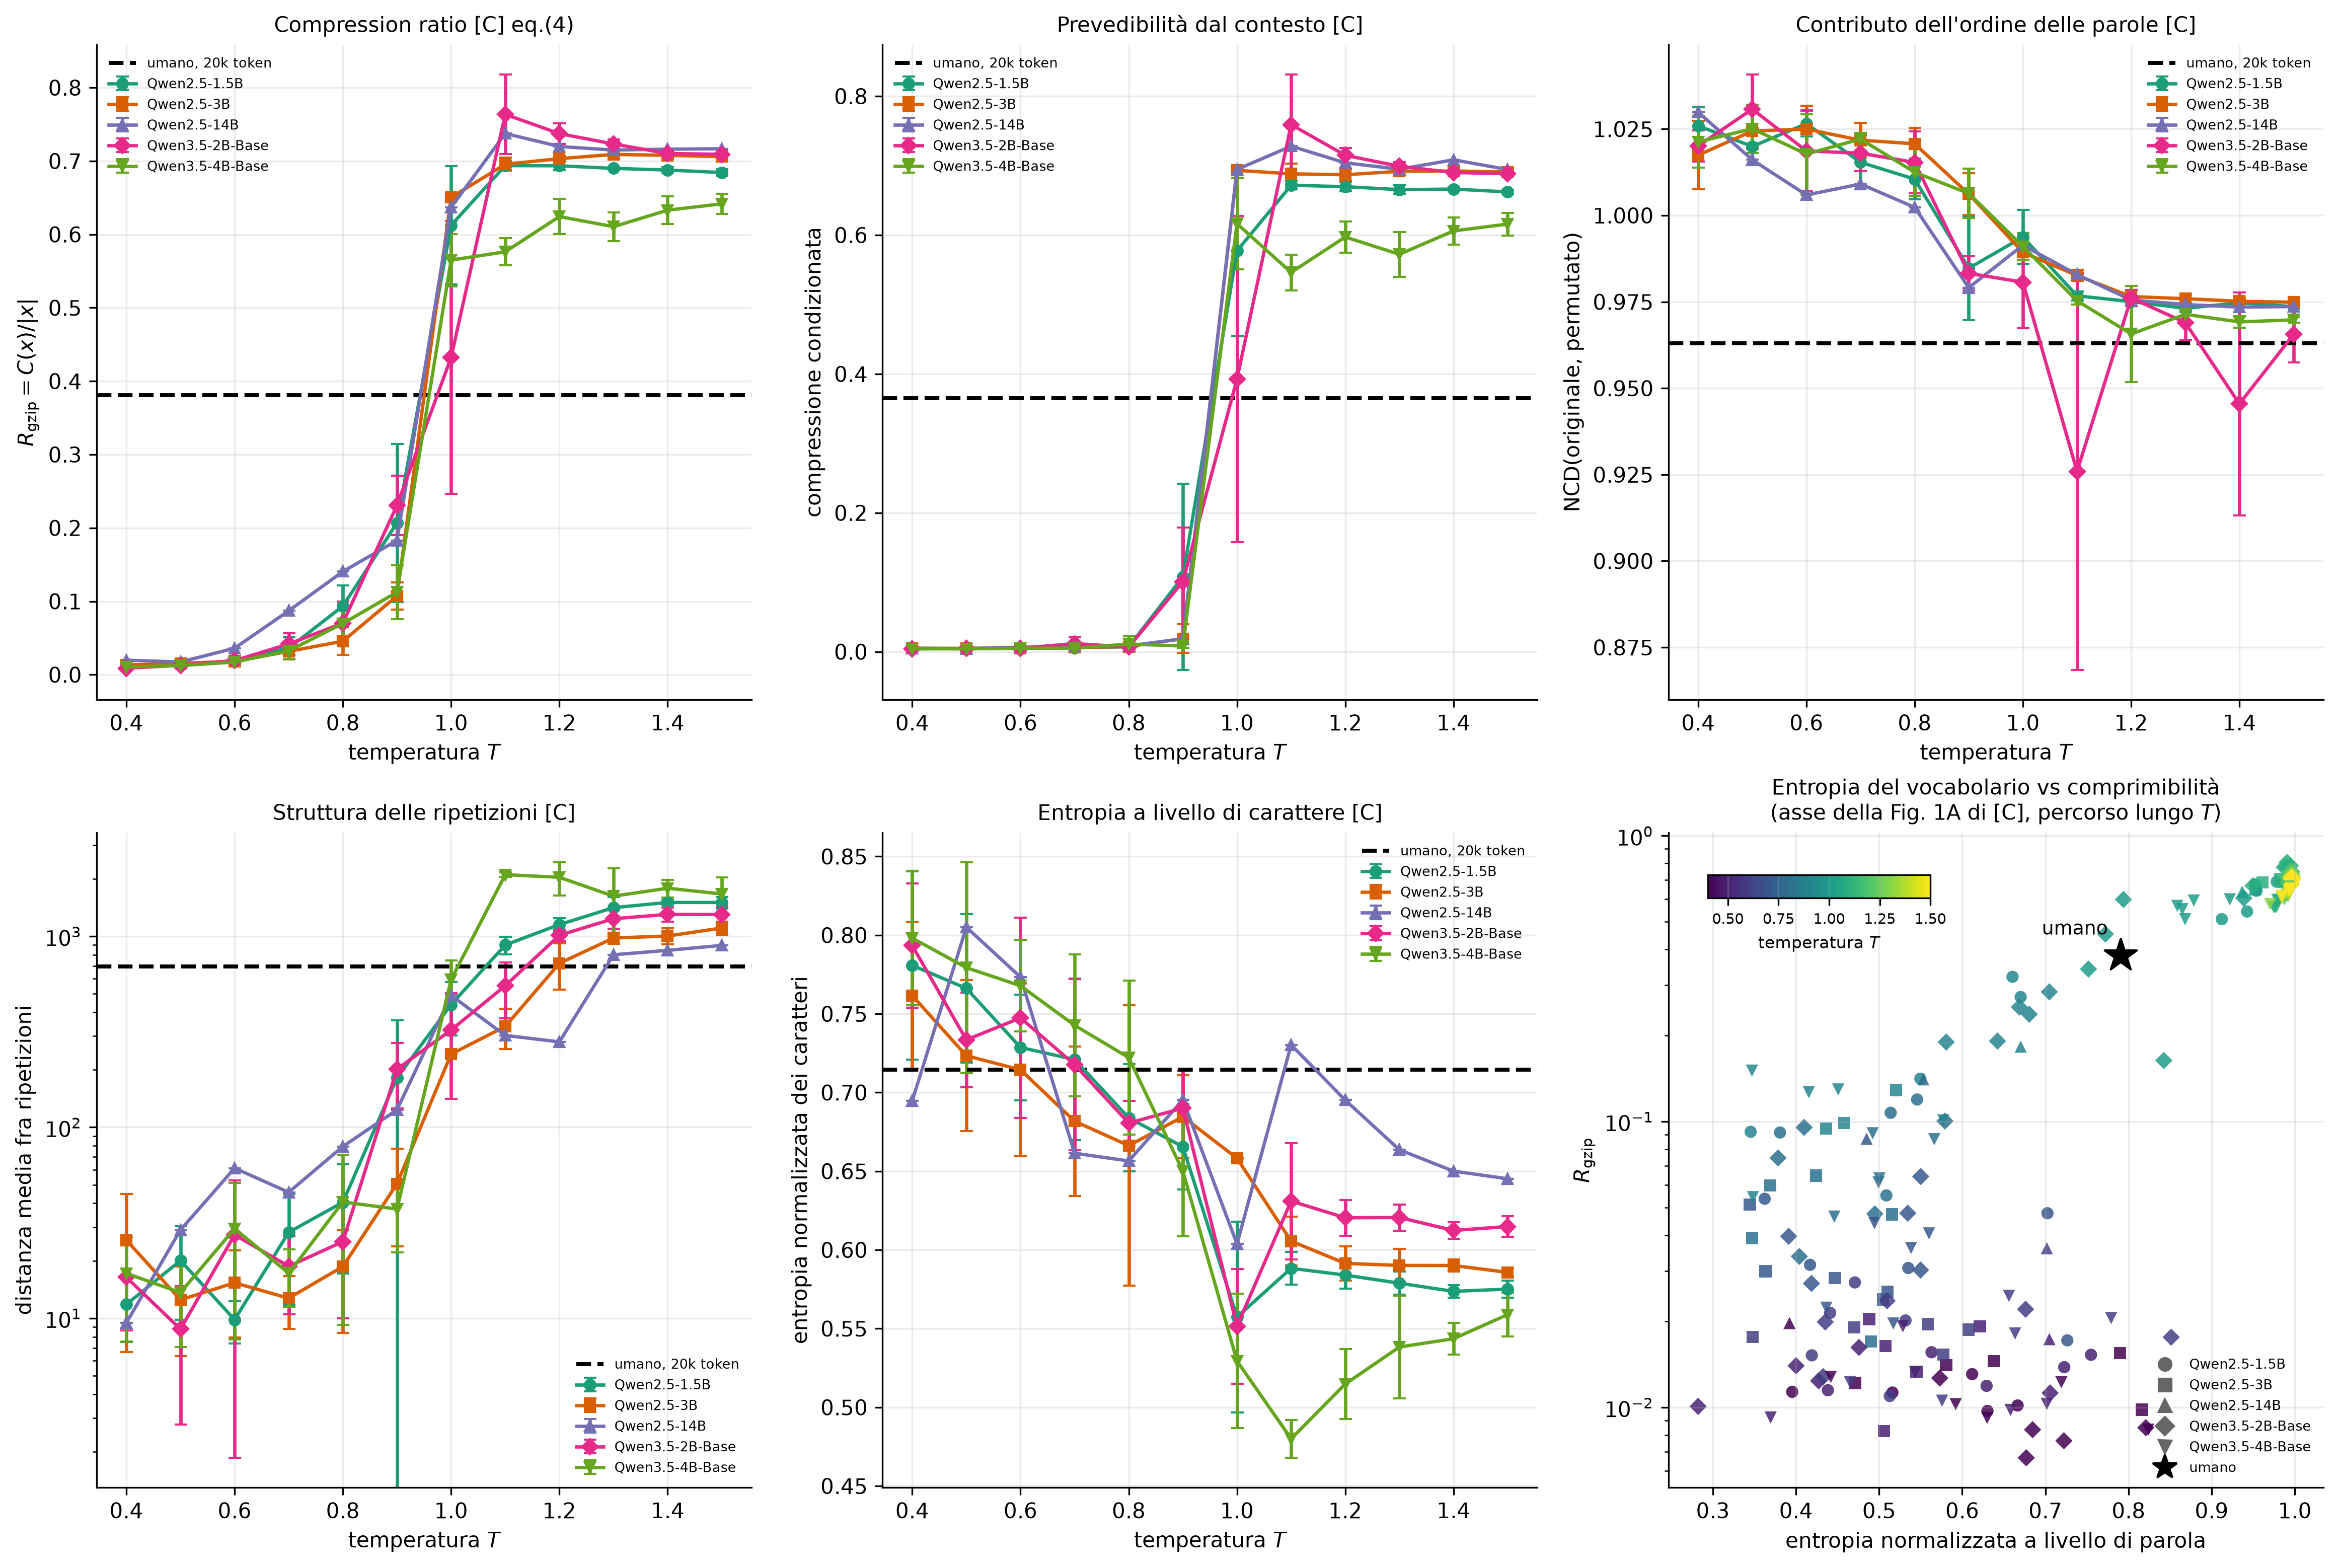
\includegraphics[width=\textwidth]{figure/cap4_compressione.png}
  \caption{Sei misure basate su compressione. Le prime cinque sono riportate in
  funzione della temperatura; l'ultima, in basso a destra, riporta il rapporto
  di compressione contro
  l'entropia normalizzata a livello di parola: è il piano della Figura~1A
  di~\cite{hadad2026}, percorso qui facendo variare la temperatura, con il testo
  umano segnato da una stella. In quel pannello il colore codifica la
  temperatura e la forma del marcatore il modello, e la scala verticale è
  logaritmica.}
  \label{fig:compressione}
\end{figure}

Il rapporto di compressione è la misura che separa i regimi in modo più netto di
tutte le altre. Per il modello esemplare passa da $0.013$ a $T = 0.4$ a $0.107$
a $T = 0.9$ e a $0.650$ a $T = 1.0$: un fattore cinquanta fra i due estremi, con
un salto di un fattore sei concentrato in un singolo passo di temperatura. Il
valore umano è $0.381$, e viene attraversato fra $T = 0.9$ e $T = 1.0$ come
tutte le altre misure del capitolo.

Il lavoro di~\cite{hadad2026} riporta che il testo generato è più regolare e
più comprimibile di quello umano, mentre qui il rapporto di compressione
supera il valore umano sopra $T = 1.0$. Le due osservazioni non sono in
contrasto, perché descrivono regioni diverse dello stesso asse: sotto la
transizione il testo generato è molto più comprimibile del testo umano,
$0.013$ contro $0.381$, ed è il regime in cui i modelli operano con le
impostazioni ordinarie; sopra la transizione la comprimibilità cade perché il
testo cessa di essere linguaggio, non perché acquisti struttura.

La compressione condizionata si comporta in modo analogo ma dice qualcosa di
diverso. Fino a $T = 0.9$ vale meno di $0.02$: la seconda metà del documento è
quasi interamente prevedibile dalla prima, come è ovvio in un testo che ripete
lo stesso ciclo. Da $T = 1.0$ sale a circa $0.69$, quasi il doppio del valore
umano $0.365$: la seconda metà è ora \emph{meno} prevedibile dalla prima di
quanto lo sia in un romanzo. Fra i due regimi non esiste una temperatura in cui
la predicibilità dal contesto assomigli a quella del testo umano.

Il salto oltre il valore umano non è una particolarità del modello esemplare. La
mediana su tutti e cinque i modelli passa da $0.015$ a $T = 0.9$ a $0.627$ a
$T = 1.0$, e il singolo modello che si avvicina di più al valore umano da sotto,
il Qwen3.5-2B-Base con $0.135$, lo scavalca comunque in un passo arrivando a
$0.430$. Nessuno dei cinque si ferma sul valore umano, ed è l'unica delle misure
di questo capitolo per cui ciò accade.

\paragraph{Il piano entropia--comprimibilità.}
Il pannello in basso a destra della Figura~\ref{fig:compressione} colloca i
documenti nel piano definito da~\cite{hadad2026}, percorso qui da un modello
reale al variare di un solo parametro anziché da distribuzioni artificiali, con
il testo umano in posizione intermedia. L'asse verticale è logaritmico perché il rapporto di compressione
non si annulla mai: il valore più basso osservato è $0.0067$. Su un asse
lineare esteso fino a $0.81$, però, i 57 documenti che stanno fra $0.007$ e
$0.020$, quasi un quarto del totale, si sovrappongono tutti sulla linea dello
zero, e la loro struttura interna scompare. In scala logaritmica si vede
invece che occupano un intervallo di entropia molto ampio, da $0.28$ a $0.85$,
e la ragione è che le due grandezze misurano cose diverse. Il rapporto di
compressione dipende dalla ripetizione della sequenza: un testo che ripete
sempre lo stesso ciclo si comprime a poco più dell'un per cento della sua
dimensione, qualunque sia il numero di parole che il ciclo contiene.
L'entropia normalizzata dipende invece dalla forma della distribuzione delle
frequenze su quel vocabolario ridotto, che conta fra 37 e 235 tipi distinti.
Un ciclo lungo e vario e un ciclo corto e povero sono ugualmente comprimibili
ma hanno entropie molto diverse: da qui la dispersione orizzontale della
nuvola a bassa comprimibilità.

\paragraph{La lunghezza del ciclo, misurata.}
L'argomento appena esposto invoca una grandezza che le misure di questo capitolo
non contengono, la lunghezza del ciclo ripetuto, ed è quindi il caso di
misurarla. Sulla successione di parole di ciascun documento si cerca il più
piccolo sfasamento $L_{\mathrm{ciclo}}$ per cui l'accordo fra la parola in
posizione $i$ e quella in posizione $i - L_{\mathrm{ciclo}}$, calcolato sugli
ultimi venti giri, supera il novanta per cento. La finestra di verifica è locale
e commisurata al periodo candidato: su tutto il testo la prosa che precede il
ciclo diluirebbe la media, mentre su un suffisso lungo un ciclo che cambia
lentamente variante scende sotto soglia al proprio periodo e la supera a un
multiplo, restituendo un alias. La soglia è fissata al novanta e non al cento
per cento per tollerare i cicli non esattamente verbatim; l'accordo atteso per
caso in prosa inglese è circa $0.05$, quindi non vi sono falsi positivi.

Il criterio individua \num{113} documenti su \num{242}, e sono tutti a
$T \le 0.9$: la totalità fino a $T = 0.7$, il $95\%$ a $T = 0.8$, il $56\%$ a
$T = 0.9$ e nessuno da
$T = 1.0$ in poi. Coincidono con la nuvola a bassa comprimibilità: tutti e
cinquantasette i documenti con $R_{\mathrm{gzip}} < 0.02$ sono fra questi. Il
ciclo va da una sola parola a \num{248}, in caratteri da $9$ a \num{1127}, con
mediana di $16$ parole.

La Figura~\ref{fig:ciclo} riporta la relazione con le due grandezze del piano.
Con l'entropia di parola la correlazione di rango vale $\rho = +0.65$, e non è
un effetto della temperatura: calcolata fra documenti generati alla stessa
temperatura sale a $+0.69$, ed è positiva in tutti e sei i gruppi. Con il
rapporto di compressione, invece, non c'è relazione: $\rho = -0.15$ con
$p = 0.12$, e a temperatura fissata il segno si inverte, $+0.16$ con
$p = 0.11$. A parità di lunghezza del ciclo il rapporto di compressione varia di
un fattore compreso fra quattordici e ventisette.

Il meccanismo è quello anticipato sopra, e la misura lo rende esplicito: la
lunghezza del ciclo coincide quasi con il numero di tipi distinti che esso
contiene, $\rho = +0.84$, cosicché un ciclo corto concentra tutta la massa di
probabilità su poche parole e uno lungo la distribuisce. Gli estremi lo
mostrano nel modo più diretto: il ciclo più corto osservato è una sola parola,
ripetuta, con entropia $0.35$; il più lungo conta \num{248} parole e undici
tipi distinti, \emph{You are a bad father. You are a bad lover of children.
You are not to blame} con variazioni, con entropia $0.47$ e $R_{\mathrm{gzip}}
= 0.019$, cioè testo ancora ultracomprimibile. La lunghezza del ciclo spiega
dunque l'ordinamento lungo l'asse orizzontale del piano, non tutta la sua
dispersione: la regressione su $\log L_{\mathrm{ciclo}}$ rende conto del
$42\%$ della varianza dell'entropia.

\begin{figure}[htbp]
  \centering
  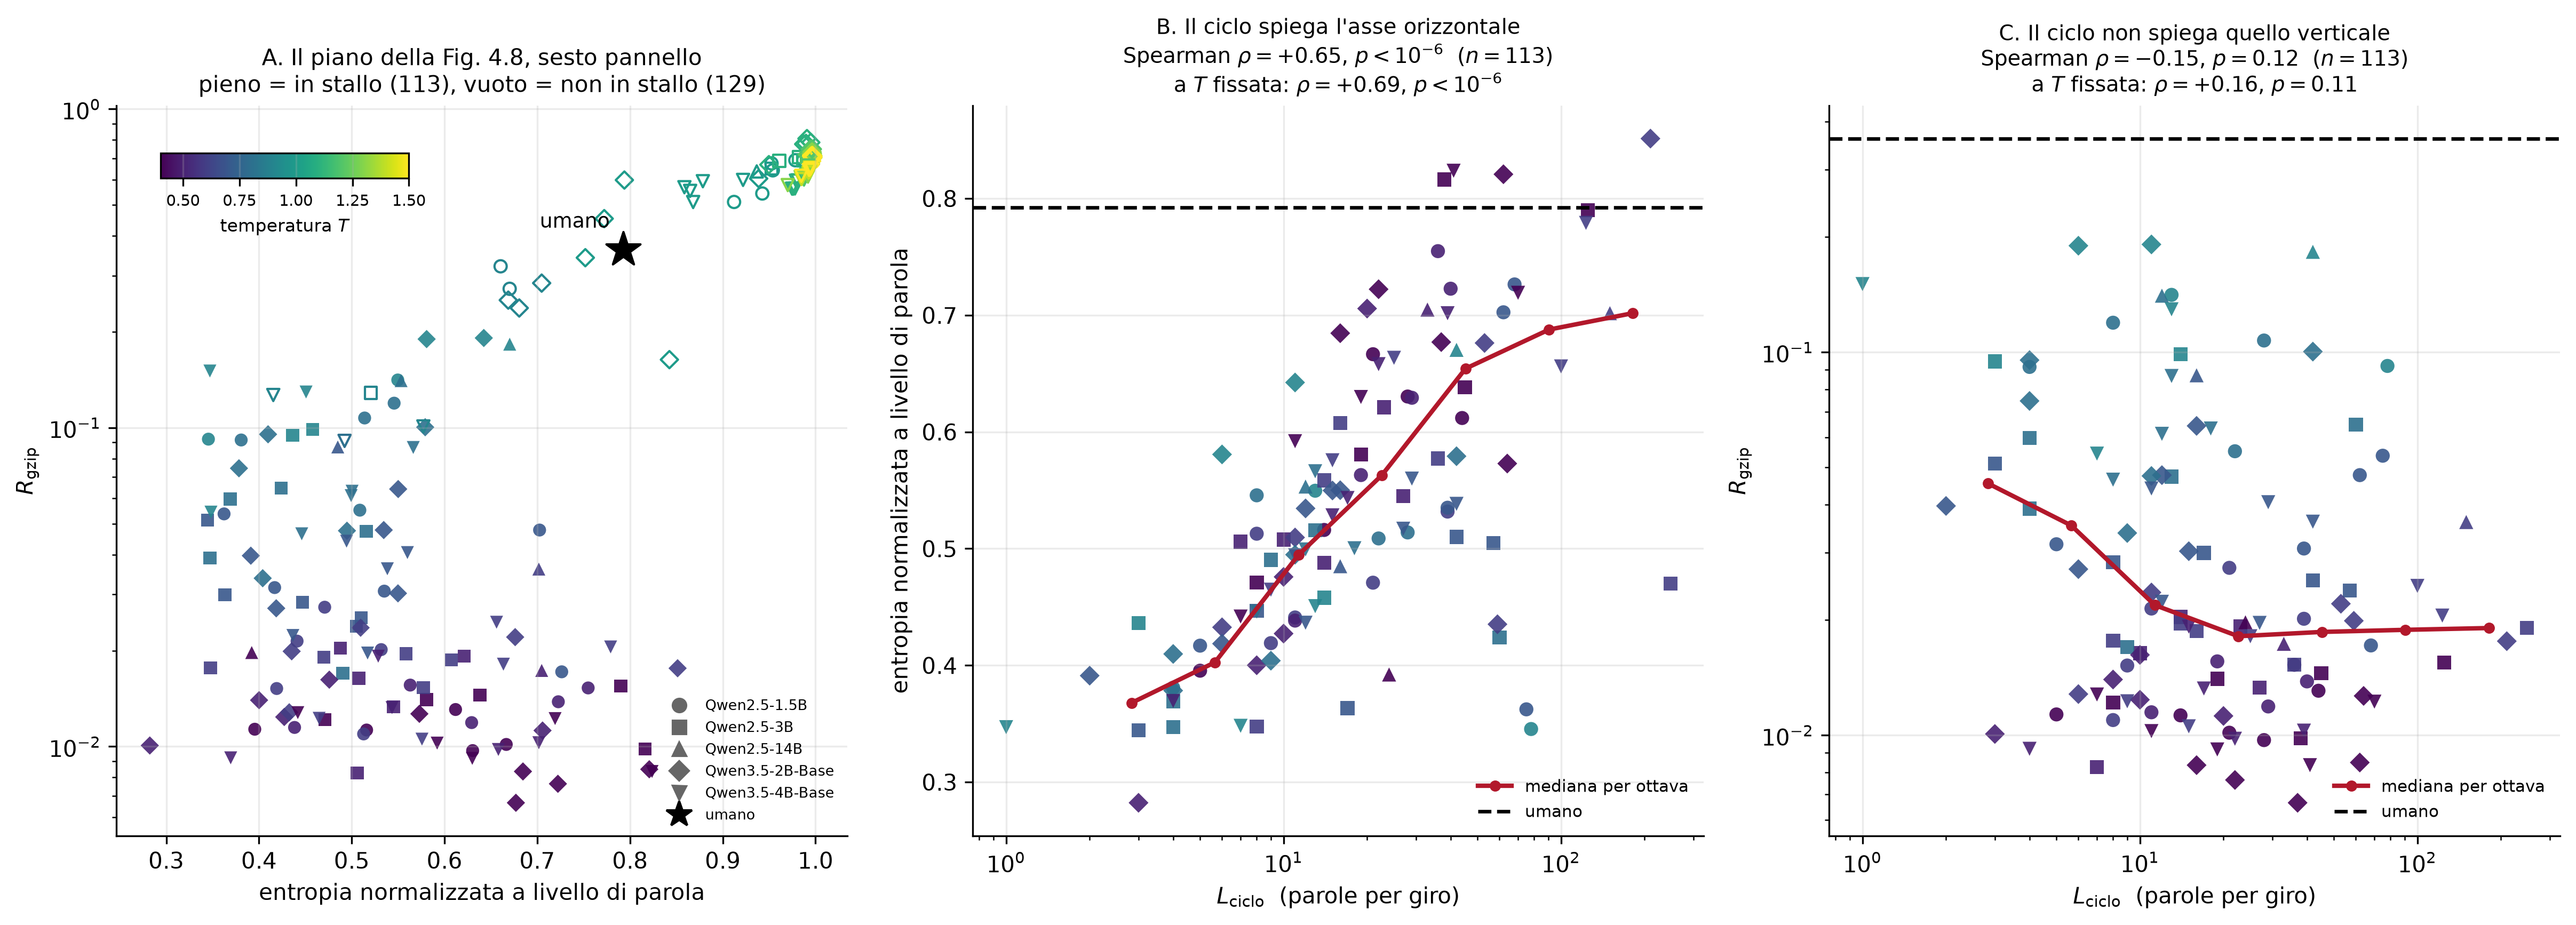
\includegraphics[width=\textwidth]{figure/cap4_ciclo_entropia.png}
  \caption{Lunghezza del ciclo ripetuto in fase di stallo. A: il piano
  entropia--comprimibilità della Figura~\ref{fig:compressione}, con i documenti
  in stallo a simbolo pieno e gli altri a simbolo vuoto; il colore codifica la
  temperatura e la forma il modello. B: entropia di parola contro lunghezza del
  ciclo, con la mediana per ottava. C: rapporto di compressione contro la stessa
  grandezza. La lunghezza del ciclo ordina l'asse orizzontale del piano e non
  quello verticale.}
  \label{fig:ciclo}
\end{figure}


% ---------------------------------------------------------------------
\section{Le tre fasi}
\label{sec:fasi-risultati}

Le misure precedenti descrivono il testo generato senza classificarlo. La regola
del §\ref{sec:tre-fasi} permette invece di assegnare ciascun documento a una
fase, e questa sezione ne riporta l'esito.

La traiettoria della~\eqref{eq:traiettoria} è costruita sui vettori GloVe a 100
dimensioni già impiegati nel §\ref{sec:token}, e l'autocorrelazione è calcolata
sui primi cento lag, misurati in parole. Il fit del GAPELMAPER usa invece un
intervallo più ampio, fino a 600 parole, perché distinguere una legge di potenza
da un esponenziale richiede più di una decade di distanze. Il livello di rumore
$\eta$ è stimato su una singola permutazione della traiettoria di ciascun
documento, con seme fissato.

Le due soglie della regola valgono $\kappa_{\min} = 0.50$ e $\Phi_{\min} = 3$.
La prima è deliberatamente permissiva: serve a escludere i documenti in cui meno
di metà delle parole ha un vettore, cioè quelli in cui la traiettoria è fatta per
lo più di zeri, e non a selezionare i documenti buoni. La seconda separa i due
gruppi in cui $\Phi$ effettivamente si distribuisce, e la sua posizione è poco
critica: come mostra la Figura~\ref{fig:transizioni}, fra la fase periodica e
quella successiva $\Phi$ cambia di due ordini di grandezza, cosicché qualunque
soglia compresa fra $1$ e $5$ produce la stessa classificazione. Il
§\ref{sec:tstar} riprende il punto trattando la fine della fase periodica come
uno degli otto criteri di temperatura critica.

La Figura~\ref{fig:acf} mostra come questa autocorrelazione cambia lungo lo
sweep. Fino a $T = 0.9$ la curva oscilla con periodo definito e ampiezza
prossima all'unità: il testo ripete un ciclo di parole, e a distanza pari a un
multiplo del ciclo ogni vettore ritrova sé stesso. Il periodo si accorcia al
crescere della temperatura, da dieci parole a $T = 0.5$ a circa tre a $T =
0.8$, mentre l'ampiezza scende da $0.98$ a $0.72$. Fra $T = 0.9$ e $T = 1.0$
la struttura periodica scompare del tutto: l'ampiezza cade a $0.036$ e la
curva diventa un decadimento monotono, senza più oscillazione. A $T = 1.3$
l'intera curva è contenuta nella banda di rumore stimata mescolando le parole
del documento, cioè non è distinguibile dal caso.

Il confronto con il testo umano chiarisce quanto entrambi i regimi siano
lontani dal linguaggio naturale. L'autocorrelazione del romanzo non è
periodica, con $\max\lvert\mathrm{FFT}\rvert$ pari a $1.16$, ben sotto la
soglia $3$, ma è nettamente sopra il livello di rumore su tutti i cento lag
esaminati, e il suo spettro decade in modo regolare invece di essere piatto.
Nessuna delle temperature campionate riproduce questa combinazione: sotto la
transizione la correlazione è troppo forte e periodica, sopra è assente.

\begin{figure}[htbp]
  \centering
  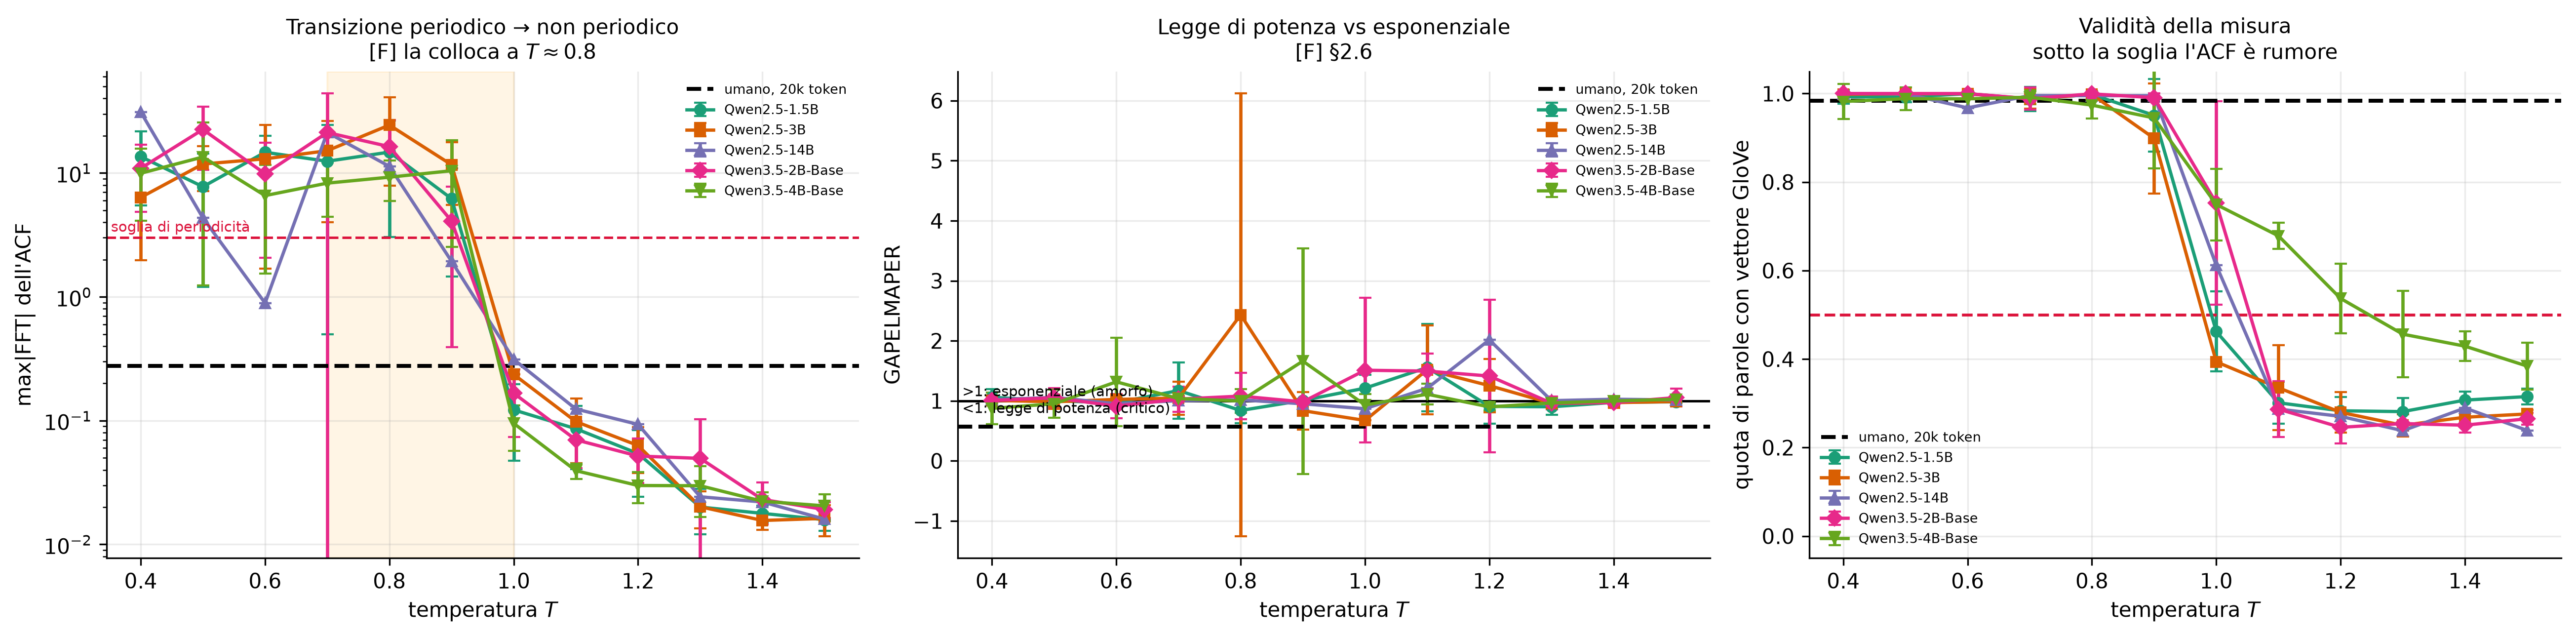
\includegraphics[width=\textwidth]{figure/cap4_transizioni_fase.png}
  \caption{Parametro di periodicità, GAPELMAPER e copertura degli embedding in
  funzione della temperatura. Il primo pannello è in scala logaritmica. Il terzo
  riporta la quota di parole dotate di un vettore, che è la condizione di
  validità delle altre due misure.}
  \label{fig:transizioni}
\end{figure}

\begin{figure}[htbp]
  \centering
  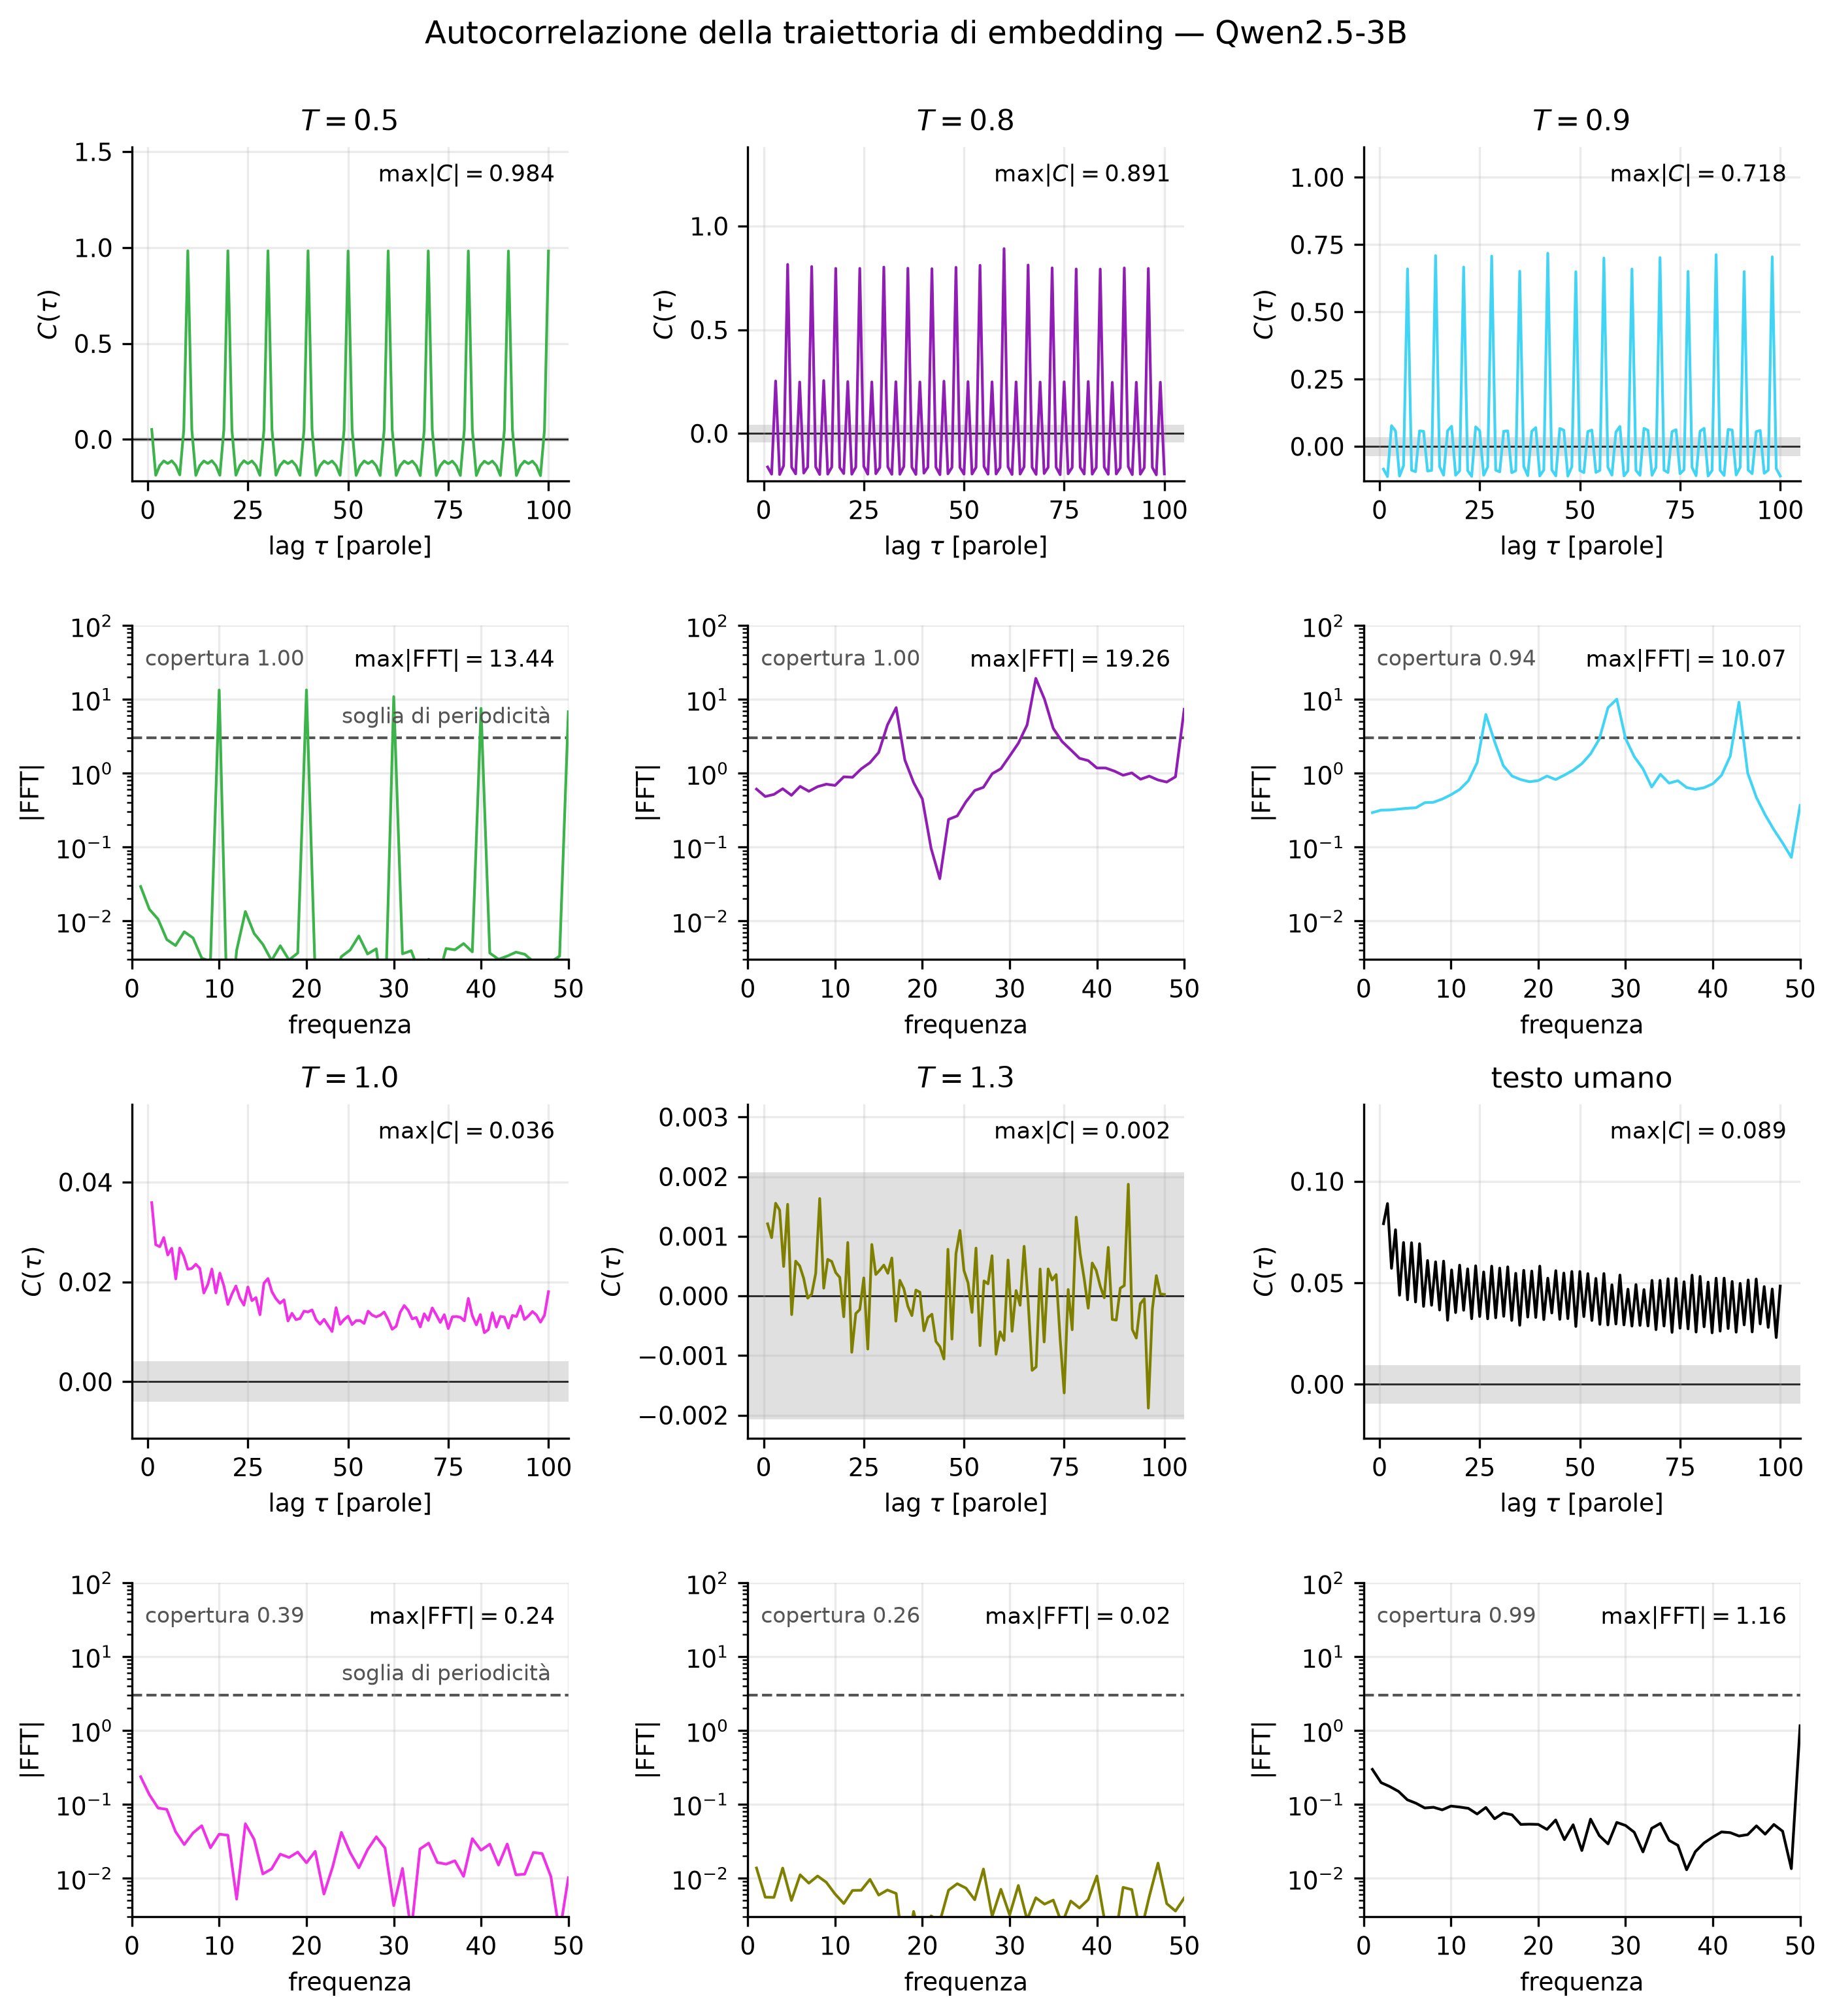
\includegraphics[width=\textwidth]{figure/cap4_acf_Qwen25_3B.png}
  \caption{Autocorrelazione della traiettoria di embedding per il modello
  Qwen2.5-3B a cinque temperature e sul testo umano di riferimento. In ciascuna
  coppia di riquadri il primo riporta $C(\tau)$ per lag da 1 a 100 parole e il
  secondo il modulo della sua trasformata di Fourier. La banda grigia è il
  livello di rumore, stimato ricalcolando $C(\tau)$ dopo aver permutato a caso
  le parole dello stesso documento; la linea tratteggiata è la soglia
  $\max\lvert\mathrm{FFT}\rvert = 3$ che separa la fase periodica. Per ogni
  temperatura è mostrato il campione di periodicità mediana, non il più marcato.
  La scala verticale di $C(\tau)$ è propria di ciascun riquadro, perché
  l'ampiezza varia di oltre due ordini di grandezza fra le temperature basse e
  quelle alte; il valore di picco è riportato dentro il riquadro. La scala dello
  spettro è invece logaritmica e comune, così i sei casi si confrontano
  direttamente.}
  \label{fig:acf}
\end{figure}

Il parametro d'ordine della prima transizione è il massimo modulo della
trasformata oltre il primo coefficiente, e il suo crollo è il risultato più
netto dell'intero capitolo. La media su tutti i modelli vale $16.0$ a
$T = 0.8$, scende a $7.5$ a $T = 0.9$ e precipita a $0.145$ a $T = 1.0$: un
fattore cinquanta in un solo passo di temperatura, e cento rispetto al massimo
di $T = 0.8$. Prosegue poi fino a $0.018$ a
$T = 1.5$, complessivamente tre ordini di grandezza sotto il massimo. Le cinque
curve dei diversi modelli si sovrappongono quasi esattamente, come mostra la
Figura~\ref{fig:transizioni}.

Anche questa soglia va confrontata con la fonte.
In~\cite{mikhaylovskiy2025states} la transizione dalla fase periodica è
collocata attorno a $t = 0.8$, con il testo dichiarato già non periodico a
$t = 1$, mentre qui la periodicità sopravvive fino a $T = 0.9$ e scompare a
$T = 1.0$. Lo spostamento verso l'alto è coerente con l'effetto del prompt
descritto nel §\ref{sec:protocollo}, che ritarda la comparsa delle proprietà
del regime disordinato.

\paragraph{Il secondo criterio non discrimina.} La distinzione fra stato
critico e fase amorfa dovrebbe essere operata dal GAPELMAPER, ma sui dati di
questo lavoro tale criterio non funziona. Il suo valore medio è $1.101$ con
deviazione standard $0.677$, e la quota di documenti con valore inferiore a 1,
cioè classificati come critici, è $0.51$: una moneta. Le barre d'errore nel
pannello centrale della Figura~\ref{fig:transizioni} sono di ampiezza
confrontabile con l'intero intervallo di variazione.

La difficoltà non è propria di questi dati. Lo stesso
\cite{mikhaylovskiy2025states} riporta che sui testi Qwen il GAPELMAPER è
raramente inferiore a 1, e che a diverse temperature del suo sweep non è
calcolabile affatto perché l'autocorrelazione assume valori negativi. Il
criterio, insomma, discrimina male anche nel lavoro che lo introduce.

Il motivo emerge dal terzo pannello. La copertura degli embedding resta sopra il
$95\%$ fino a $T = 0.9$, ma crolla a $0.64$ a $T = 1.0$ e a circa $0.31$ oltre
$T = 1.2$: nel regime in cui il GAPELMAPER dovrebbe distinguere le ultime due
fasi, l'autocorrelazione è calcolata su una minoranza delle parole e non
contiene più segnale. Per questa ragione i documenti che non superano la soglia
di copertura sono marcati come non valutabili anziché classificati, come
anticipato nel §\ref{sec:tre-fasi}. Senza tale precauzione il criterio avrebbe
assegnato una fase a documenti in cui non c'è nulla da misurare.

\paragraph{Il diagramma di fase.}
La Figura~\ref{fig:diagramma} riporta la composizione delle fasi per modello e
temperatura. Il quadro è coerente su tutti e cinque: fase periodica fino a
$T = 0.9$, dove la classificazione è ancora periodica per 13 documenti su 18;
scomparsa completa della periodicità a $T = 1.0$; documenti prevalentemente non
valutabili da $T = 1.1$ in poi, e completamente tali a $T \ge 1.4$.

\begin{figure}[htbp]
  \centering
  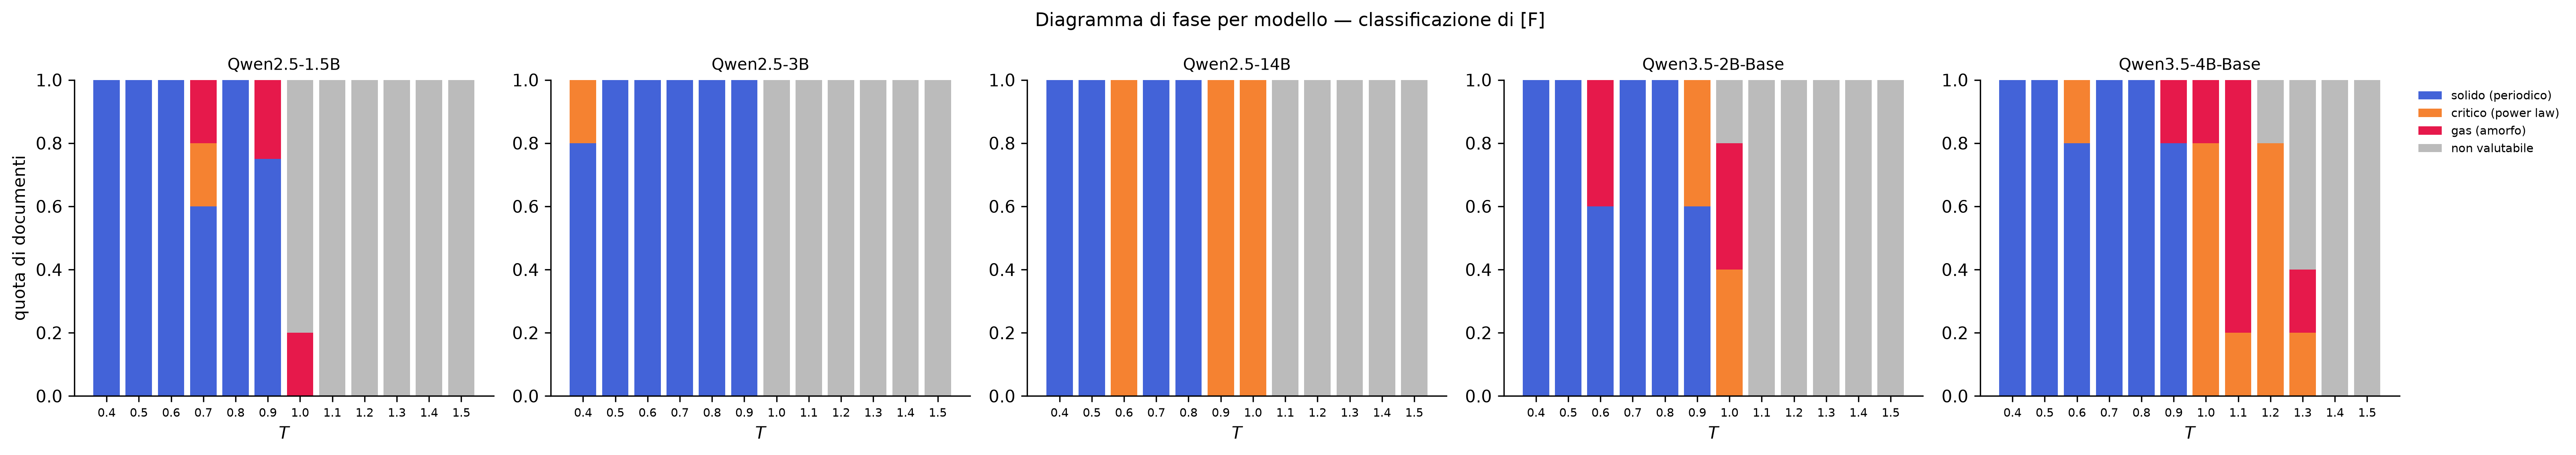
\includegraphics[width=\textwidth]{figure/cap4_diagramma_fase.png}
  \caption{Composizione delle fasi per modello e temperatura. La categoria «non
  valutabile» raccoglie i documenti che non superano la soglia di copertura
  degli embedding.}
  \label{fig:diagramma}
\end{figure}

Le tre modalità di fallimento del §\ref{sec:fallimenti} trovano qui la loro
interpretazione. La degenerazione per ripetizione è la fase periodica; la
degenerazione dell'alfabeto e del lessico corrisponde alla regione in cui la
misura non è più applicabile, che è a sua volta il segnale della fase amorfa. Il
testo non degenerato esiste solo nella striscia sottile fra le due, ed è la
stessa striscia in cui tutte le misure delle sezioni precedenti si avvicinano ai
valori umani.

% ---------------------------------------------------------------------
\section{Convergenza della temperatura critica}
\label{sec:tstar}

Le sezioni precedenti individuano ciascuna una temperatura privilegiata. Poiché
i criteri provengono da lavori indipendenti e misurano proprietà diverse del
testo, il loro accordo o disaccordo è esso stesso un risultato.

La Tabella~\ref{tab:tstar} riporta la temperatura selezionata da ciascun
criterio per ciascun modello. Due criteri sono intrinseci, nel senso che
individuano un estremo della curva senza far riferimento al testo umano: il
minimo del MAPE e la fine della fase periodica. Gli altri sei selezionano la
temperatura alla quale la misura si avvicina di più alla baseline umana.

\begin{table}[htbp]
\centering
\small
\begin{tabular}{@{}lccccc@{}}
\toprule
Criterio & 1.5B & 3B & 14B & 3.5-2B & 3.5-4B \\
\midrule
MAPE minimo                                  & 0.9 & 0.9 & 0.7 & 0.9 & 0.9 \\
$D_s$ minima dal testo umano                 & 0.9 & 0.9 & 0.9 & 0.9 & 1.0 \\
Fine della fase periodica                    & 1.0 & 1.0 & 0.6 & 1.0 & 1.0 \\
$R_{\mathrm{gzip}}$ più vicino all'umano     & 0.9 & 1.0 & 0.9 & 1.0 & 1.0 \\
$\alpha$ più vicino all'umano                & 1.0 & 1.5 & 1.3 & 1.0 & 1.0 \\
$R$ più vicino all'umano                     & 1.0 & 1.1 & 1.1 & 1.1 & 1.0 \\
$\gamma_H$ più vicino all'umano              & 1.1 & 1.0 & 1.3 & 1.1 & 1.3 \\
$\alpha_{\mathrm{DFA}}$ più vicino all'umano & 1.2 & 1.1 & 1.1 & 1.1 & 1.1 \\
\midrule
\textbf{mediana}                             & \textbf{1.0} & \textbf{1.0} &
\textbf{1.0} & \textbf{1.0} & \textbf{1.0} \\
\bottomrule
\end{tabular}
\caption{Temperatura selezionata da ciascun criterio, per ciascun modello. La
mediana vale $1.0$ per tutti e cinque i modelli, benché i singoli criteri
spazino da $0.6$ a $1.5$.}
\label{tab:tstar}
\end{table}

Il risultato principale del capitolo è la riga in fondo alla tabella. Otto
criteri tratti da quattro lavori indipendenti, costruiti per scopi diversi e mai
progettati per concordare, danno una mediana identica per tutti e cinque i
modelli. La convergenza non era scontata: i criteri misurano la distribuzione
delle frequenze, la crescita del vocabolario, le correlazioni a lungo raggio, la
comprimibilità e la periodicità dell'autocorrelazione, cioè proprietà che nulla
obbliga a coincidere.

\begin{figure}[htbp]
  \centering
  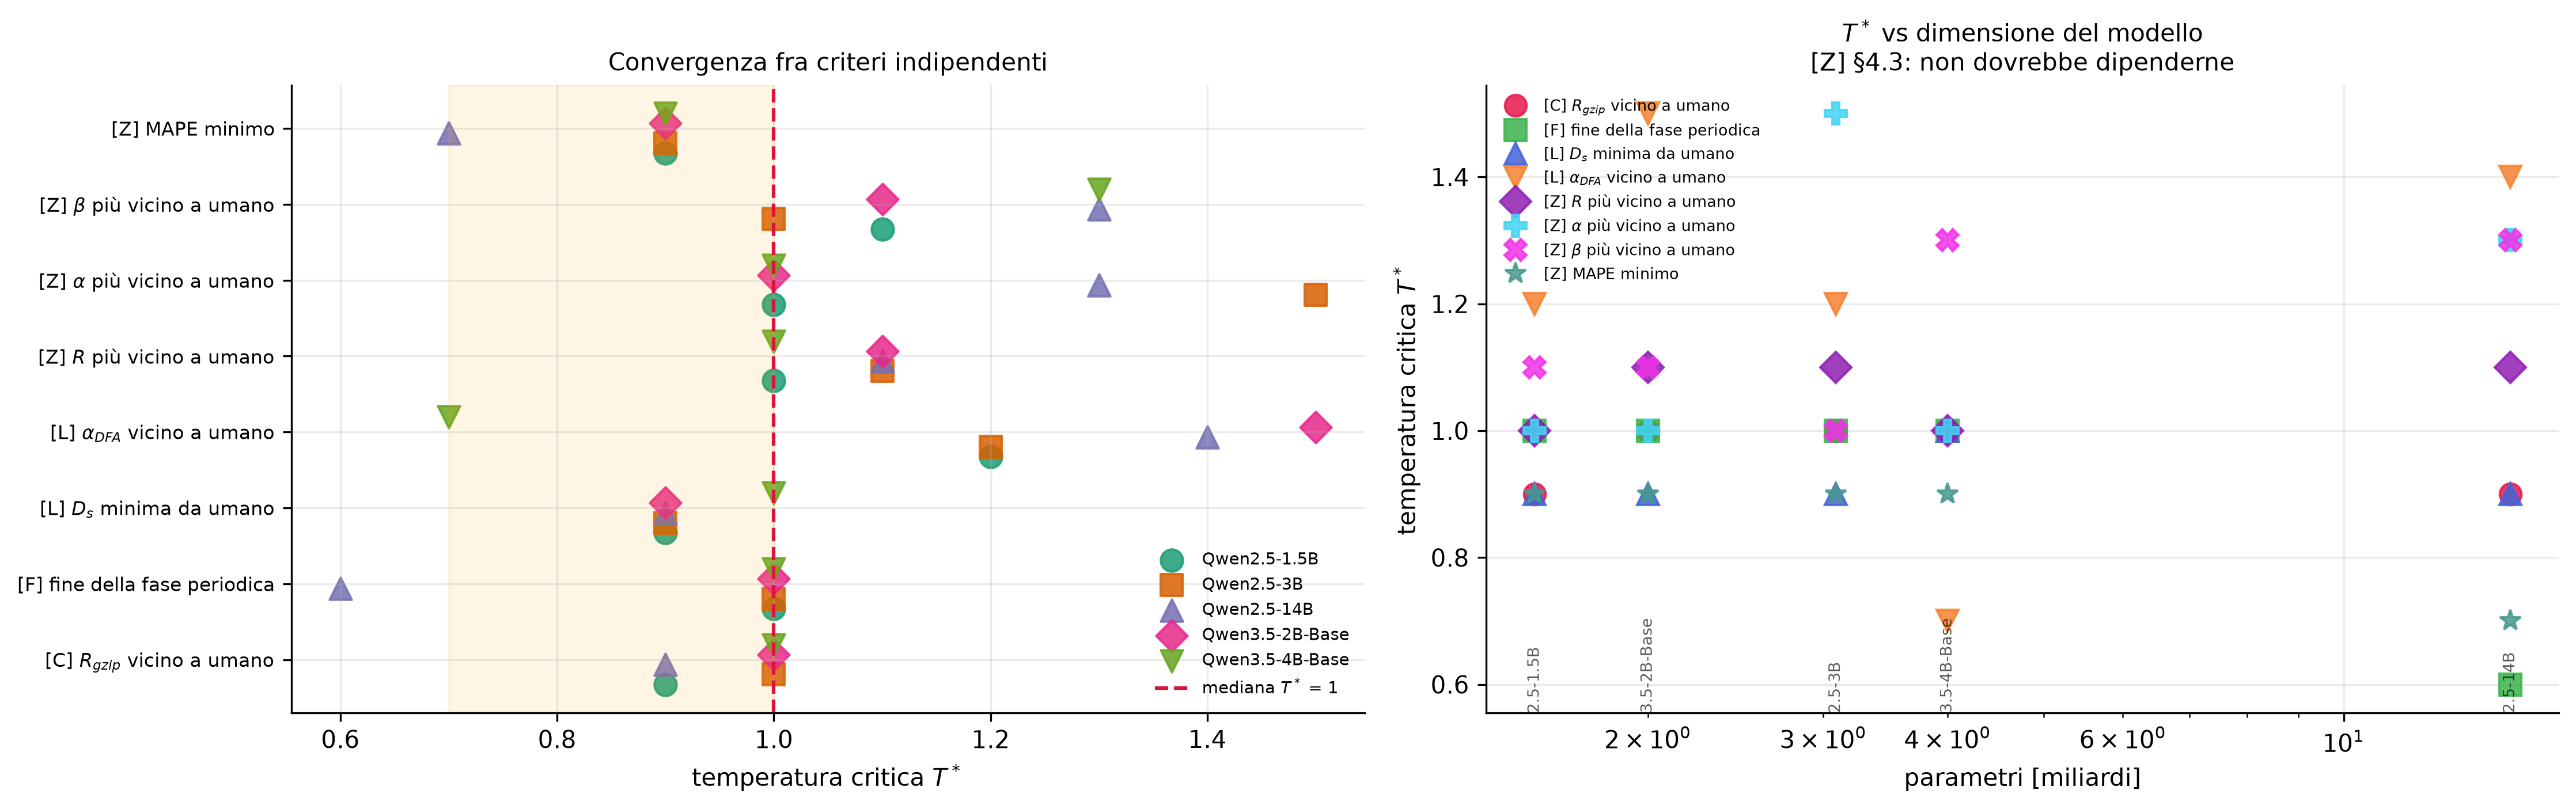
\includegraphics[width=\textwidth]{figure/cap4_temperatura_critica.png}
  \caption{A sinistra, la temperatura selezionata da ciascun criterio; la linea
  tratteggiata è la mediana complessiva e la banda la regione fra $0.7$ e $1.0$.
  A destra, la stessa quantità in funzione del numero di parametri del modello.}
  \label{fig:tstar}
\end{figure}

\paragraph{Dipendenza dalla dimensione del modello.}
La Figura~\ref{fig:tstar} riporta a destra la temperatura critica in funzione
del numero di parametri. La correlazione di rango è $\rho = -0.01$ con
$p = 0.93$ su quaranta osservazioni: nessuna dipendenza rilevabile. Il dato è
coerente con quanto riportato in~\cite{mikhaylovskiy2025zipf}, dove la posizione
dell'ottimo risulta indipendente dalla dimensione per tutte le famiglie
esaminate.

Un'assenza di correlazione misurata su cinque modelli appartenenti a due
famiglie non dimostra l'indipendenza: dimostra che, entro l'intervallo di
dimensioni esplorato e con la potenza statistica disponibile, non emerge
alcuna dipendenza. È coerenza con la letteratura, non conferma indipendente.

\paragraph{Una discordanza fra criteri.}
Due criteri si collocano sistematicamente fuori dal gruppo, e la loro distanza
dagli altri è essa stessa un risultato: mediarli insieme al resto la
cancellerebbe.

Il minimo del MAPE cade a $0.9$, mentre la fine della fase periodica cade a
$1.0$: alla temperatura in cui la distribuzione delle frequenze è più vicina a
una legge di potenza, l'autocorrelazione è ancora periodica per la maggioranza
dei documenti. Le due misure non si contraddicono, perché guardano oggetti
diversi, la statistica dei conteggi l'una e la struttura sequenziale l'altra,
e la loro distanza quantifica il fatto che le due proprietà non compaiono
simultaneamente. Il testo acquista una distribuzione di frequenze verosimile
prima di perdere la ripetizione.

Il criterio basato su $\alpha_{\mathrm{DFA}}$ merita una nota, perché il suo
esito dipende dall'ordine del detrending. Con il grado 1 seleziona temperature
fra $0.7$ e $1.5$, il più disperso dei nove; con il grado 2, che è quello
adottato qui per la ragione data nel §\ref{sec:robustezza}, si allinea agli
altri e sceglie $1.1$ per quattro modelli su cinque. La mediana per modello vale
$1.0$ in entrambi i casi. Resta valida l'avvertenza del
§\ref{sec:dfa-risultati}: alle basse temperature quell'esponente è instabile
fra documenti, e viene riportato per completezza anziché usato come criterio a
sé stante.

Una divergenza analoga fra criteri è documentata
in~\cite{mikhaylovskiy2025zipf} per i modelli Llama di grandi dimensioni, dove
le leggi di Zipf e di Heaps individuano temperature critiche sensibilmente
diverse. Il fenomeno non sembra dunque un artefatto di questo lavoro.

% ---------------------------------------------------------------------
\section{Che cosa lo sweep ha stabilito}
\label{sec:sintesi-cap4}

Tre risultati emergono dalle sezioni precedenti, di natura diversa fra loro.

Il primo è l'esistenza di una temperatura privilegiata, e la sua posizione. Otto
criteri costruiti per scopi diversi e tratti da quattro lavori indipendenti
danno una mediana identica, $T = 1.0$, per tutti e cinque i modelli, senza
dipendenza rilevabile dalla dimensione. Il secondo è che l'ottimo è stretto: la
transizione si consuma quasi interamente fra $T = 0.9$ e $T = 1.0$, dove il
parametro di periodicità cade di un fattore cinquanta, l'entropia passa da
$0.332$ a $5.77$ bit per carattere e il rapporto di compressione da $0.107$ a
$0.650$. Uno sweep a passo $0.1$ è appena sufficiente a risolvere quella
finestra.

Il terzo è l'esito negativo su cui poggia il capitolo successivo. L'esistenza
dell'ottimo è un fatto generale, ma la sua \emph{qualità} non lo è: due modelli
su cinque portano il MAPE al livello del testo umano e gli altri no. La
compressione condizionata non raggiunge il valore umano a nessuna temperatura,
ma per una ragione che non riguarda la struttura semantica: sotto la transizione
il testo ripete un ciclo e la seconda metà è prevedibile per costruzione, sopra
non è più linguaggio e non è prevedibile da nulla. Soprattutto, i documenti che
superano tutte e tre le soglie di non
degenerazione sono due su \num{242}. Il corpus generato lungo lo sweep non
sostiene quindi un'analisi semantica, ed è la ragione per cui il
Capitolo~\ref{cap:risultati2} cambia dominio anziché proseguire su questo.

Il capitolo non stabilisce però tutto. La convergenza dei criteri dice dove il
testo generato somiglia di più a quello umano secondo misure che ignorano il
significato; non dice se in quel punto il testo sia organizzato attorno a un
contenuto. È la domanda posta nel §\ref{sec:intro-domanda}, e richiede gli
strumenti del §\ref{sec:burst}.